\documentclass[12pt]{report}
\usepackage[a4paper,
    left=0.7in,
    right=0.7in,
    top=1.5in,
    bottom=1in,
    headheight=15pt,
    headsep=0.5in,
    footskip=0.5in
]{geometry}
\usepackage{fancyhdr}
\usepackage{tabularx}
\usepackage{enumitem}
\usepackage{tocloft}
\usepackage{booktabs}
\usepackage{graphicx}
\usepackage[T1]{fontenc}
\usepackage{lmodern}

\usepackage{ragged2e}
\usepackage[table]{xcolor}
\usepackage[plainpages=false,pdfpagelabels,hypertexnames=false,colorlinks=true,linkcolor=blue,citecolor=blue,urlcolor=blue]{hyperref}
\hypersetup{
    pdfborderstyle={/S/U/W 1},
    allbordercolors=blue
}
\usepackage{tikz}
\usepackage{dashrule}
\usepackage{setspace}
\usepackage{titling}
% Format chapter heading
\usepackage{titlesec}
\usepackage{algorithm}
\usepackage{algpseudocode}
\usepackage{amsmath}
\usepackage{longtable}             % For longtable environment
\usepackage{textcomp}
\usepackage{float}                 % For [H] float placement
\usepackage{rotating}              % For landscape/sideways figures
\usepackage[strings]{underscore}   % Handle underscores in text
\DeclareUnicodeCharacter{2212}{-}                         % minus sign
\DeclareUnicodeCharacter{2264}{\ensuremath{\leq}}         % ≤
\DeclareUnicodeCharacter{2194}{\ensuremath{\leftrightarrow}}

\makeatletter
\newenvironment{breakablealgorithm}
   {\begin{center}
     \refstepcounter{algorithm}
     \hrule height.8pt depth0pt \kern2pt
     \renewcommand{\caption}[2][\relax]{%
       {\raggedright\textbf{Algorithm \thealgorithm} ##2\par}%
       \ifx\relax##1\relax
         \addcontentsline{loa}{algorithm}{\protect\numberline{\thealgorithm}##2}%
       \else
         \addcontentsline{loa}{algorithm}{\protect\numberline{\thealgorithm}##1}%
       \fi
       \kern2pt\hrule\kern2pt
     }
   }
   {\kern2pt\hrule\relax
    \end{center}}
 \makeatother
% Chapter Formatting
\titleformat{\chapter}[display]
  {\centering\bfseries\fontsize{18}{20}\selectfont}
  {Chapter \thechapter}
  {0pt}
  {}

\titlespacing*{\chapter}
  {0pt}
  {0pt}
  {12pt}



% Enable deep numbering
\setcounter{secnumdepth}{3}
\setcounter{tocdepth}{3}


% Header & Footer Setup
\pagestyle{fancy}
\fancyhf{} % clear all header and footer fields

% Header
\fancyhead[L]{\small COMSATS University Islamabad}
\fancyhead[R]{\small Final Year Project}

% Footer
\fancyfoot[C]{\thepage}
\renewcommand{\headrulewidth}{0.4pt}
\renewcommand{\footrulewidth}{0pt}

% Suppress overfull/underfull hbox warnings for table content
\tolerance=1000
\hbadness=10000
\emergencystretch=3em
\hfuzz=2pt

\begin{document}
\hypersetup{pageanchor=false}
\begin{titlepage}
    \centering
    % University Name
    {\Large \textbf{COMSATS University Islamabad, Vehari Campus, Pakistan} \par}
    \vspace{0.3cm}
    {\large Department of Computer Science \par}
    \vspace{0.7cm}
    % Thesis Title
    {\Large \textbf{Lets Go Ride Sharing App} \par}
    \vspace{0.7cm}
    % Logo
    
\includegraphics[width=0.30\textwidth]{logo.png}
    \vspace{0.7cm}
    
    % Degree Statement
    {\large  A Thesis Submitted in Partial Fulfillment of the Requirements
        for the Degree of \par}

    \vspace{0.5cm}
    {\Large \textbf{Bachelor of Science in Software Engineering} \par}
    \vspace{1cm}
    % Candidate Information
    \large\textbf{Submitted By} \par
    \vspace{0.5cm}
    {\large
    ALI RAZA \hspace{0.3cm} (FA22-BSE-116) \par
    M.FAWAD SAQLAIN \hspace{0.3cm} (FA22-BSE-031) \par
    }
    \vspace{0.5cm}
    % Supervisor Information
    \large\textbf{Supervisor} \par
    \vspace{0.5cm}
    \large DR Syeda Zoupash Zahra \par
    \vspace{0.5cm}
    \large{Session: Fall 2022-2026 \par}
    
\end{titlepage}
\newpage
% ---------- Roman numbering ----------
\hypersetup{pageanchor=true}
\pagenumbering{roman}
\setcounter{page}{1}
\pagestyle{plain}
% File: dedication.tex

\newpage
\thispagestyle{empty}

\begin{center}
\textbf{\LARGE Dedication}
\end{center}

\vspace{1cm}

\begin{spacing}{1.5}

To my mother and father for their unwavering support, sacrifices and prayers, this has been a success theirs and mine. They have helped me on my way through these times with encouraging words, patience and a firm belief in me.
I also acknowledge this to my teachers and mentors who inspired me to devote myself to the search of knowledge in integrity.

\end{spacing}

\newpage
  
% File: acknowledgement.tex

\newpage
\thispagestyle{empty}

\begin{center}
\textbf{\LARGE Acknowledgement}
\end{center}

\vspace{1cm}

\begin{spacing}{1.5}

All praise and gratitude are due for the successful completion of this project. The authors would like to express their sincere appreciation to their supervisor for continuous guidance, valuable suggestions, and constructive feedback throughout the development of this thesis. The supervision and mentorship provided significant support in completing this work successfully.

Special thanks are extended to the faculty members of the Department of Computer Science for their academic support and encouragement during the degree program.

The authors are also deeply grateful to their parents and families for their unwavering support, motivation, and prayers, which have been a constant source of strength.

Finally, appreciation is extended to everyone who directly or indirectly contributed to the successful completion of this project.

\end{spacing}

\newpage
 

% File: certificate.tex

\newpage
\thispagestyle{empty}

\begin{center}
\textbf{\LARGE Certificate of Approval}
\end{center}

\vspace{1.5cm}

\begin{spacing}{1.5}

This is to certify that the Final Year Project titled 
\textbf{``Lets Go Ride Sharing App''} 
has been developed by \textbf{Ali Raza (FA22-BSE-116)} and \textbf{Fawad Saqlain (FA22-BSE-031)} under the supervision of \textbf{DR. SYEDA ZOUPASH ZAHRA} and that in her opinion, the project is adequate in scope and quality for the award of the degree of  Bachelor of Science in Software Engineering.

\end{spacing}

\vspace{2.5cm}
\noindent\rule{6cm}{0.4pt}  
\\ 
Supervisor

\vspace{2.5cm}
\noindent\rule{6cm}{0.4pt}  
\\ 
External Examiner

\vspace{2.5cm}

\noindent\rule{6cm}{0.4pt}  
\\ 
Head of Department  
\\ 
Department of Computer Science

\newpage

\input{plagiarism}
% File: executive_summary.tex

\newpage
\thispagestyle{plain}

\addcontentsline{toc}{section}{Executive Summary}

\begin{center}
\textbf{\LARGE Executive Summary}
\end{center}

\vspace{1cm}

\begin{spacing}{1.5}

The urban transportation system is also evolving dramatically, as its provision of efficient, cost-effective, and reliable transport options is becoming more in-demand in urban areas, especially in those experiencing rapid growth, around the world. Modem society has introduced numerous problems to commuters, including over long wait times, high ticket prices, and the larger societal problems of excessive traffic and pollution. Although ride-hailing has been a game-changer, it has also added new inefficiencies (requiring drivers to get ‘wisely lost' on the way to passengers to the detriment of costs, fuel and environmental impact), and is unlikely to be disappearing soon. The project, known as “Lets Go Ride Sharing App” comes as a smart solution to these problems especially for the socio-economic and cultural setting of Pakistan. Through cutting edge mobile technology and intelligent matching algorithms the system seeks to change into the concept of ride-sharing by selecting to connect on a route based upon matching, as opposed to on-demand dispatch which drivers on commute have traditionally resorted to during the low efficiency part of their day.

The core issue that Lets Go Ride Sharing App is designed to solve is the inefficiency of current transportation solutions, which typically have low passenger loads and a large and rising demand. Many conventional services fail to identify the opportunities for sharing the cost among users of service who are travelling in the same direction, not to mention the missed opportunities for much economic savings and environmental care. Additionally, social sensitivities and cultural norms, especially gender preferences, are often never taken into consideration by the global platforms, which is a limitation for a lot of potential users in the Pakistani playbook who prioritize personal comfort and cultural relevance while traveling. Underutilised cars also have an environmental impact, as each new vehicle added to the road will be responsible for increasing the levels of CO2, air pollution, and urban smog. Both are addressed by a sophisticated feature of the Lets Go Ride Sharing App that takes priority in matching people with vehicles—the ability to overlap routes—in order to match a passenger with a driver's existing travel plans, which maximises efficiencies and reduces unnecessary deviation.

A key aspect of Lets Go Ride Sharing App is its backend, which has been built with Python's Django framework, making it scalable, stable, and offering real-time data processing.The Django-based Python backend is another core feature of Lets Go Ride Sharing App, providing a scalable, stable, and high-quality real-time data processing experience. The architecture lies on eight system modules ranging from thorough user verification to real-time ride matching, secure transparent pricing algorithms to suggestions based on machine learning. In contrast to traditional pricing models with a predetermined structure, the pricing in Lets Go Ride Sharing App will be an agreement reached between all users focusing on the distance traveled and the fuel used, as well as the pricing to be negotiated between users. This "mixed" approach is transparent and accountable, and it's fair to the local commuters' financial circumstances and their bargaining power. Safety is handled with a multi-layer of verification for CNIC, driving licenses; real-time location tracking, SOS at all times. Another key addition is the NLP-driven chatbot, which not only enhances the user experience but also delivers instant help, addresses common after-mentioned questions, and simplifies intricate platform requirements for new users.

Lets Go Ride Sharing App now takes the technology much further to the data science and user interaction point. Passenger history, travel preferences and passenger ratings from past trips are thoroughly examined with the help of a content based recommendation system, which picks out the most suitable and compatible ride options. Such personalization also allows users to not only get a ride on the same path as those they can access in their area, but to ride on the same path suitable for their own safety and comfort level, including the important aspect of gender matching for riders and drivers. The system helps in an effective car pooling system, which reduces the number of vehicles on road leading to a considerable decrease in urban carbon footprint and assists in reducing the urban issues such as traffic congestion, especially in densely populated cites. On the socio-economic side, being able to share travel costs means that the university student, the office worker and everyday professional alike will have access to a local solution to commute that is much more accessible and affordable, than the international one which is more focused on profit than direct benefit to his own community.

As a comprehensive solution is being developed, the project follows the software development life cycle, including testing and validation. 481 automated tests were not only integrated, but 281 for the Flutter application were added, along with 199 for the Django application, to ensure that every functionality, from login to fare calculation, is reliable and is sufficiently robust. The platform is well documented with Software Requirements and Software Design Specifications that clearly indicate future scalability and maintainability. It is implemented as a web-based interface in the administrative panel and gives seamless control over the entire ecosystem, with users' verification, dispute resolution and financial analytics easily managed by the administrators. The comprehensive development strategy guarantees that the Lets Go Ride Sharing App doesn't only serve their functional purpose, but can become a robust software system that can support an expanding user base.

To sum up the Lets Go Ride Sharing App is a comprehensive solution, addressing the mobility challenges faced by modern urban transportation. It effectively harnesses the balance and synergy between the high-tech software engineering and local cultural relevance thereby creating an affordable, safe and sustainable environment for the modern Pakistani commuter. The project presents a sophisticated usage of the skills in full stack development, machine learning, natural language processing, and an understanding of real-world challenges in urban transportation. As the Lets Go Ride Sharing App continuously adapts to user needs and evolves with its community, it will potentially make a significant impact on Pakistan's transportation landscape to become more efficient, safer, and sustainable.

\end{spacing}
\newpage
% File: abbreviations.tex

\newpage
\thispagestyle{plain}

\begin{center}
\textbf{\LARGE Abbreviations}
\end{center}

\vspace{1cm}

\begin{table}[htbp]
\centering
\renewcommand{\arraystretch}{1.4}
\begin{tabularx}{\textwidth}{|p{3cm}|X|}
\hline
\textbf{Abbreviation} & \textbf{Full Form} \\
\hline
\textbf{SRS} & Software Requirements Specification \\ \hline
\textbf{SDD} & Software Design Document \\ \hline
\textbf{API} & Application Programming Interface \\ \hline
\textbf{UI} & User Interface \\ \hline
\textbf{DB} & Database \\ \hline
\end{tabularx}
\end{table}

\newpage

\newpage

\renewcommand*\contentsname{Table of Contents}
\tableofcontents
\newpage
\addcontentsline{toc}{section}{List of Tables}
\listoftables

\newpage
\addcontentsline{toc}{section}{List of Figures}
\listoffigures

\clearpage
% ---------- Arabic numbering ----------
\pagenumbering{arabic}
% ==============================
% Chapter 1 – Introduction
% ==============================

\chapter{Introduction}

% --------------------------------
% 1.1 Introduction
% --------------------------------

\section{Introduction}

With the development of this society, there is a lot of demand for cheap, fast transportation that is suitable for the current society's needs. Efficient and reliable. The urban commuter has a lot of challenges such as waiting times,High prices, congestion and environmental issues from overuse of the vehicle. Traditional forms of transport and current ride-hailing services have not been meeting the demand for ride-hailing well. Address these concerns, creating a pressing need for innovative solutions.

Ride-hailing services like Careem, Uber, and Bykea dominate the industry and intercity carpooling platforms like BlaBlaCar are dominant in the transportation industry. These solutions have transformed personal mobility but of course have their limitations. Most traditional ride-hailing services work by sending drivers to pick up passengers from. At certain places, often with diversions from normal routes. This a lack of an operational model leads to more time delays, more fuel, more fares for passengers, After accounting for operational costs, however, drivers' earnings were lower and their employment rate was lower after the introduction of the system.

Other issues that have been identified with the current transportation solutions are the lack of proper sharing of expenses, with platforms rarely addressing matching those who are already travelling. The same direction. The importance of cultural sensitivities is often overlooked, and traditional models fail to consider them. Gender preferences to a greater extent in areas where there is already a particular cultural norm.Further, extra charges and late deliveries happen as vehicles get off the beaten track in order to pick up passengers, While the impact of the environment is not being addressed, with more vehicles on the roads, adding to that impact. Reduce pollution and congestion on the roads.

The need of the hour is to eradicate these gaps by creating a platform that matches passengers with drivers who are on the same path.The proposed “Lets Go Ride Sharing App” aims to address these gaps by matching passengers with drivers on similar routes. Unlike traditional services which send Lets Go Ride Sharing App helps drivers find a friend out of their way by matching those who are travelling in the same direction within the same area, in order to share the ride and expenses.This approach not only saves on transportation costs but also helps promote environmental sustainability by minimizing the number of vehicles on the road. The system is equipped with high-tech features. With robust user verification, gender preferences, and live route matching, it enhances the safety and accessibility of the platform.It improves the safety and accessibility of the platform with comprehensive user verification, gender preferences, and live route matching. Flexible payment methods suitable for the Pakistani audience, instant chatbot support, and personalized ride recommendations through machine learning. By combining technological innovation with cultural sensitivity, Lets Go Ride Sharing App presents a comprehensive solution to the inefficiencies plaguing current transportation systems.

% --------------------------------
% 1.2 Vision Statement
% --------------------------------

\section{Vision Statement}

Lets Go Ride Sharing App aims to revolutionize urban commuting in Pakistan by creating a sustainable, cost-effective, and culturally sensitive ride-sharing ecosystem that connects passengers with drivers traveling along identical routes. The target users include daily commuters within local communities such as office workers, university students, and residential area residents who seek affordable and reliable transportation options while minimizing their environmental footprint.

The core problem this system intends to solve is the inefficiency inherent in traditional ride-hailing services, where drivers must deviate from their routes, causing delays and increased costs for all parties. By facilitating true ride-sharing among users already heading in the same direction, Lets Go Ride Sharing App eliminates unnecessary detours, reduces individual transportation expenses, and decreases the number of vehicles on roads.

The long-term vision is to use the Lets Go Ride Sharing App as the preferred mode of transportation for commuters. A secure and culturally diverse platform, known for its focus on user safety, cultural relevance and environmental responsibility. The platform aims to play an important role in the alleviation of urban Reduce traffic congestion and carbon dioxide emissions and provide access to transportation and affordable transport services for To all sections of society.

The innovation lies in combining route-based matching with gender-based preferences, hybrid Clear pricing, enabling mutual fare deals, and machine learning-driven personalisation. It is a one-of-a-kind combination of attributes, from an aspect of practical transportation to one of health and safety. Cultural issues that are not being addressed through the current global platforms, which puts Lets Go Ride in a new light. Sharing App as a truly localised solution with global best practices.

% --------------------------------
% 1.3 Related System Analysis
% --------------------------------

The ride sharing and transportation platform includes many of the established platforms that are in existence. Different methods and restrictions. This part examines three major systems relevant to. The suggested Lets Go Ride Sharing App program.

\textbf{BlaBlaCar} is an intercity long-distance carpooling service focused in Europe and others. Other regions which are not available in Pakistan. The platform allows drivers to link up with empty vehicles. To passengers between cities, for long distance journeys, they can share the cost. BlaBlaCar’s main Key features include verified user profiles, trusted payment systems, and community-based ratings. Some of its drawbacks are that it is mainly used for intercity travel and not daily commute in urban areas, it is not available in the Pakistani market and the lack of support for short distance travel with it. Cultural preference options such as gender-based matching.

\textbf{InDrive} is a ride-hailing service with a unique feature that enables passengers to negotiate directly with drivers. Users make their own suggestion and drivers select Whether or not to accept the offer. This model offers pricing flexibility but it's very much a negotiating model and not really much about ecient route matching.

\textbf{Bykea} is a Pakistan-based motorcycle ride-hailing service focused on urban mobility, particularly in major cities like Karachi, Lahore, and Islamabad. The platform offers affordable transportation, parcel delivery, and bike rentals. Bykea has successfully localized its services for the Pakistani market with cash payments and affordable pricing. However, its limitations include a primary focus on motorbike transportation rather than car-based ridesharing, lack of true expense-splitting features for passengers traveling the same direction, and limited attention to gender-based preferences and comprehensive safety verification.

The proposed Lets Go Ride Sharing App application addresses these limitations through several key improvements. Unlike BlaBlaCar's intercity focus, Lets Go Ride Sharing App targets both short and long urban commutes within local communities. In contrast to InDrive's negotiation-only approach, Lets Go Ride Sharing App combines transparent fare calculation with mutual agreement while actively matching users based on overlapping routes. Compared to Bykea's motorbike model, Lets Go Ride Sharing App implements car-based ridesharing for expense splitting, incorporates gender-based preferences, and emphasizes environmental impact through reduced vehicle counts.

\begin{table}[htbp]
\centering
\caption{Comparative Analysis of Existing Systems}
\renewcommand{\arraystretch}{1.3}

\begin{tabularx}{\textwidth}{|p{3cm}|X|X|}
\hline
\textbf{Application Name} & \textbf{Identified Weaknesses} & \textbf{Proposed Improvements} \\
\hline
BlaBlaCar &
\begin{itemize}[leftmargin=*, noitemsep, topsep=0pt]
    \item Primarily focuses on intercity long trips
    \item Not available in Pakistan
    \item Limited support for short-distance travel
    \item Lacks cultural preference features
\end{itemize}
&
\begin{itemize}[leftmargin=*, noitemsep, topsep=0pt]
    \item Matches users on similar routes for both short and long commutes
    \item Designed specifically for Pakistani market
    \item Supports daily urban commuting
    \item Allows gender-based preferences
\end{itemize}
\\
\hline
InDrive &
\begin{itemize}[leftmargin=*, noitemsep, topsep=0pt]
    \item Relies on fare negotiation only
    \item Does not focus on route matching
    \item Lacks cultural sensitivities
    \item No true ridesharing feature
\end{itemize}
&
\begin{itemize}[leftmargin=*, noitemsep, topsep=0pt]
    \item Provides transparent fare calculation with mutual agreement
    \item Links users with overlapping routes
    \item Integrates gender-based preferences
    \item Enables expense sharing through ride matching
\end{itemize}
\\
\hline
Bykea &
\begin{itemize}[leftmargin=*, noitemsep, topsep=0pt]
    \item On-demand motorbike service
    \item No true ridesharing or cost-sharing
    \item Limited verification and safety features
    \item Lacks gender preference options
\end{itemize}
&
\begin{itemize}[leftmargin=*, noitemsep, topsep=0pt]
    \item Route-based carpooling for expense splitting
    \item Reduces environmental impact through fewer vehicles
    \item Comprehensive user verification
    \item Gender-based matching for cultural sensitivity
\end{itemize}
\\
\hline
\end{tabularx}
\end{table}

% --------------------------------
% 1.4 Project Deliverables
% --------------------------------

The Lets Go Ride Sharing App mobile application project will produce the following tangible Outputs are software modules, documentation artefacts, and implementation deliverables.

\textbf{List of Deliverables:}

\begin{enumerate}
    \item \textbf{Registration \& Verification Module} – A comprehensive user registration system, which supports Drivers \& Passengers. This module gathers and validates the user data. Name, Phone number, e-mail, Post office address, CNIC, driving license, Vehicle. registration details. The features include role switching between driver and passenger, and two-factor authentication to ensure extra security.
    
    \item \textbf{Ride Request \& Acceptance Module} – Facilitates communication between drivers and passengers by making available a variety of services: ride requests, real-time notifications, fare estimates and more.Ride progress updates. Has an explicit and clear cancellation policy with conditions.
    
    \item \textbf{Payment \& Fare Calculation Module} – Provides all payment and fare calculations with hybrid. Transparent pricing. The system automatically recommends the fare according to distance, fuel costs, It allows drivers and passengers to see, adjust and agree to, margins and profits without worrying about each other. Agree on final fares. Accepts cash and online bank transfer as payment method, manually verification of transactions.
    
    \item \textbf{Safety \& Security Module} – Provides user safety through integration with emergency contacts, real-time location tracking and manual verification of all user information such as identity. Documents and driving papers.
    
    \item \textbf{Rating \& Review Module} – Provides an opportunity for feedback after the ride is completed. A rating system and written reviews that are combined to create user profiles and trust within the community.
    
    \item \textbf{Administrative \& Reporting Module} – An extensive online interface where administrators can regulate user verification, settle disputes, review monetary analytics and handle, etc. Account management functions.
    
    \item \textbf{Chatbot Module} – Supplies instant support to the user through a natural language processing interface with automatic answers and escalation to live support if required.
    
    \item \textbf{Machine Learning Module} – Implements content-based recommendation systems to personalize ride suggestions based on user travel preferences, history, and other parameters. Includes predictive analytics for fare adjustments and route optimization.
    
    \item \textbf{Software Documentation} – Complete project documentation including Software Requirements Specification (SRS), Software Design Document (SDD), test cases, user manuals, and API documentation for future maintenance and scalability.
    
    \item \textbf{Deployed Application} – Fully functional mobile application build deployed for testing and demonstration purposes. The delivered build is distributed as an Android APK, while iOS distribution is planned as future work.
\end{enumerate}

% --------------------------------
% 1.5 System Limitations / Constraints
% --------------------------------

The Lets Go Ride Sharing App mobile application, while comprehensive in its design, operates within certain limitations and constraints that must be acknowledged for realistic project expectations.

\begin{itemize}
    \item \textbf{Dependence on User Participation:} The effectiveness of ride matching depends heavily on a critical mass of active users. With a small user base, efficient ride matching becomes difficult, potentially leading to limited ride options for passengers and fewer passenger requests for drivers during the initial deployment phase.

    \item \textbf{Reliance on Third-Party Services:} The application depends on external mapping APIs for location tracking and route calculation, as well as LLM APIs for chatbot integration. Service downtime, API changes, or rate limitations imposed by these third-party providers may temporarily affect application functionality and user experience.

    \item \textbf{Internet Connectivity \& Location Accuracy:} Real-time features including ride matching, location tracking, and fare calculation require stable internet connectivity and accurate GPS data. Users in areas with poor network coverage or inaccurate GPS signals may experience degraded performance or inability to use core features.

    \item \textbf{Security \& Verification Overheads:} The thorough manual verification process for user documents (CNIC, driving license, vehicle registration) enhances safety but may slow down the registration process. New users might face delays before they can fully utilize the platform, which could affect user acquisition and retention.

    \item \textbf{Payment Gateways:} The current scope does not include integration with automated online payment gateways. Transactions rely on cash and manual verification of bank transfers, which may introduce delays in payment confirmation and requires additional administrative overhead for payment reconciliation.

    \item \textbf{Geographic Scope:} Initial deployment is limited to specific local communities and urban areas. Rural regions and smaller cities may not be served during the initial phases, limiting the application's reach and accessibility.

    \item \textbf{Time and Resource Constraints:} As an academic project with defined timelines, certain advanced features or extensive scalability testing may be deferred to future iterations. The development team comprises two students, limiting development capacity and specialization.
\end{itemize}

% --------------------------------
% 1.6 Tools and Technologies
% --------------------------------

\section{Tools and Technologies}

The Lets Go Ride Sharing App mobile application leverages a carefully selected technology stack for compatibility across platforms, performance on the backend, efficient data handling, and scalable architecture. Specific project needs and constraints guide each technology choice.

\textbf{Frontend Development:} Flutter with Dart SDK is chosen for cross-platform mobile app development so that one codebase can be used for both Android and iOS platforms. This saves development time and effort while keeping native-like performance and a smooth user experience on all devices. Flutter's widget library also provides ample scope to implement the user-friendly interface required by the project.

\textbf{Backend Development:} Python with Django offers a powerful, scalable, and secure backend framework. Django's security features, ORM, and template system help development while promoting good authentication and access control practices. The implemented backend uses Django 6.0.5 as per the project dependency, and the test environment uses Python 3.12.

\textbf{Database Management:} PostgreSQL is used as the main database for real-time data management, offering reliability, ACID compliance, and support for complex queries needed for route matching and user data management. Its JSON support allows it to be used flexibly with diverse data structures across different modules.

\textbf{Administrative Interface:} HTML5, CSS3, and JavaScript are used to create the web-based administrative interface, which is responsive and user-friendly for administrators to manage users, track transactions, and settle disagreements.

\textbf{External APIs:} Maps API integration allows route visualization, distance calculation, and real-time location tracking for fare estimation. LLM API integration powers the chatbot module for natural language understanding and automatic user support.

\textbf{Machine Learning:} Python machine learning libraries such as scikit-learn and TensorFlow enable the development of content-based recommendation systems, predictive analytics, and personalized ride suggestions.

\begin{table}[htbp]
\centering
\caption{Tools and Technologies Used in the Project}
\renewcommand{\arraystretch}{1.3}
\begin{tabularx}{\textwidth}{|p{4cm}|p{3cm}|X|}
\hline
\textbf{Tool / Technology} & \textbf{Version} & \textbf{Purpose} \\
\hline
Flutter (Dart SDK) & Latest stable & Cross-platform mobile app development for iOS and Android \\
\hline
Python & 3.12 & Backend programming language \\
\hline
Django & 6.0.5 & Python web framework for backend implementation \\
\hline
PostgreSQL & Latest stable & Real-time data management and storage \\
\hline
HTML5 & N/A & Admin panel interface structure \\
\hline
CSS3 & N/A & Admin panel interface styling and design \\
\hline
JavaScript & ES6+ & Admin panel client-side validation and functionality \\
\hline
Maps API & N/A & Location tracking, route visualization, distance calculation \\
\hline
LLM API & N/A & Chatbot integration for natural language processing \\
\hline
Machine Learning Libraries & Latest & Predictive analytics and content-based recommendations \\
\hline
\end{tabularx}
\end{table}

% --------------------------------
% 1.7 Relevance to Course Modules
% --------------------------------


The Lets Go Ride Sharing App project shows full-fledged integration of academic application experience from the knowledge gained during the Bachelor of Science in Software Engineering program, resulting in the ability to apply theory to practice.

\subsection{Programming Fundamentals}

The project uses basic programming logic and principles of object-oriented programming in all modules. Classes and objects represent real-world objects like users, vehicles, routes, and rides. Encapsulation helps to ensure data integrity in each module of the application, inheritance helps in code reuse in similar cases, and polymorphism provides flexibility in dealing with different user roles and components. Modular concepts and practices are followed in the separation of concerns across the modules that form the system. Each feature has clearly defined interfaces. Good coding style, such as sensible naming, properly formatted conventions, indentation, and detailed comments, supports maintainability and readability.

\subsection{Data Structures and Algorithms}

Proper data management is essential for route matching and ride recommendations. The project uses suitable data structures such as hash maps for fast user lookups, queues for ride request maintenance and processing, and graphs for route representation and optimization. Search algorithms facilitate efficient matchmaking of passengers with drivers according to shared routes. Sorting algorithms present ride listings based on relevance, distance, and time. Optimization techniques minimize route deviations and reduce computational complexity for real-time updates. Machine learning algorithms look at travel patterns for personalized recommendations.

\subsection{Database Management Systems}

Database design is based on normalization principles that eliminate data redundancy and ensure data integrity. An entity-relationship diagram is used to describe relationships between users, vehicles, rides, payments, and reviews. PostgreSQL uses these relationships through well-formulated tables, primary keys, foreign keys, and indexes to optimize queries. Complex SQL queries fetch rides according to location and time, based on user preferences. Transaction management guarantees consistency of data throughout the payment system and ride confirmation. Database security measures are implemented to protect detailed user information such as CNIC and license details.

\subsection{Software Engineering}

The project is intended to be a full Software Development Life Cycle from requirements gathering through deployment. The scope document is the initial requirement engineering artifact; it captures functional and non-functional requirements rather than being the final result. UML diagrams such as use case diagrams, class diagrams, and sequence diagrams show how the system behaves and is structured. The modularity follows sound software engineering practices such as separation of concerns and high cohesion with low coupling. Testing strategies include unit testing and integration testing for module interactions. Complete SRS, SDD, and user manuals follow standard templates and standards. Agile principles govern development in an iterative manner with continuous feedback incorporation.

\subsection{Other Relevant Courses}

\textbf{Artificial Intelligence:} The module on machine learning is a content-based recommendation system that uses AI concepts to make the user experience more personal based on travel history and preferences. Predictive analytics identify demand patterns and pricing optimization.

\textbf{Human-Computer Interaction:} User interface design uses HCI principles to ensure simple navigation, good user experience, and user-friendliness. Mockups and prototypes are tested for usability before implementation.

\textbf{Web Development:} The administrative panel takes advantage of full-stack web development skills, using HTML5, CSS3, and JavaScript for the frontend and Django for backend API integration.

\textbf{Cybersecurity:} Measures such as two-factor authentication, secure data storage, and privacy protection are in line with cybersecurity principles, ensuring the protection of user information and preventing unauthorized access.

\textbf{Software Project Management:} The Gantt chart and milestone planning are related to project management objectives such as timeline estimation, task allocation, and progress monitoring within defined constraints.

This chapter introduced the background and context of the proposed Lets Go Ride Sharing App system, highlighting the challenges of high costs, inefficiencies, and cultural insensitivities in existing transportation solutions. The vision and strategic objectives of the system were outlined to establish its intended impact as a cost-effective, culturally sensitive, and environmentally sustainable commuting platform for Pakistani users. A comparative analysis of related systems including BlaBlaCar, InDrive, and Bykea identified key limitations such as lack of route matching, absence of gender-based preferences, and limited local focus. Project deliverables encompassing the core software modules, supporting features, and comprehensive documentation were specified. System constraints including dependence on user participation, third-party services, and internet connectivity were acknowledged. Selected technologies with Flutter, Python Django, PostgreSQL, and various APIs were justified for their suitability. The academic relevance demonstrated integration of knowledge from Programming Fundamentals, Data Structures, Database Systems, Software Engineering, and other courses. This chapter establishes the foundation for the detailed problem definition presented in the next chapter.
  
% ==============================
% Chapter 2 – Problem Definition
% ==============================

\chapter{Problem Definition}

% --------------------------------
% 2.1 Problem Statement
% --------------------------------

\section{Problem Statement}
As the society got advanced people get increasing need for a fast, economical and reliable transportation system which is both cheap and affordable. The urban commuters are confronted with various issues like lengthy waiting periods, high fares, congestion in the city streets, environmental issues due to excessive use of vehicles etc. These issues have never been so effectively solved with traditional modes of transport and existing ride-halters and it's clear that something new is needed.

The market is dominated by ride hailing solutions like Careem, Uber and Bykea, as well as intercity carpooling solutions BlaBlaCar, which also meets people's mobility needs. These services are drivers of change in the way people travel, but with significant shortcomings. Typical ride-haling services typically send drivers to pick up riders at certain spots, where they are likely to be forced off their routes. The consequences of this are lengthy delays, more fuel spent, more money collected by the passengers and less for the drivers once the operating costs are taken into account.

A significant problem is also inadequate mechanisms for share of expenses. Unlike most platforms, most services do not pay special attention to matching people when they are on parallel journeys so to decrease transportation costs. Cultural considerations are also ignored often, especially gender preferences that are significant in such areas of Pakistan. Moreover, additional pickups delay and increase vehicle cost, environmental effects are still serious as there are more vehicles on road means more pollution and congestion.

These problems impact on everyday commuters who require affordable transportation, drivers who would like to look for out options to turn away from unnecessary maneuvers to do business and the broader community that suffers from pushing street traffic.Those are problems for everyday commuters who need affordable transportation, drivers who would prefer to search for methods to deviate from pointless route changes, and the general public which suffers from traffic congestion and air pollution. These are not trivial issues, but rather factors that contribute to low efficiency and low utilization of sustainable transit opportunities.

% --------------------------------
% 2.2 Proposed Solution Overview
% --------------------------------

\section{Proposed Solution Overview}

The Lets Go Ride Sharing App is a ride sharing mobile application by which any passenger and driver who travels along similar route will be connected to get the ride, thereby changing the way commuting works in local communities. Unlike other traditional services that dispatch drivers to random destinations, Lets Go Ride Sharing App pairs people who are already travelling in the same direction, and share the trip and expenses.

The envisioned system tackles with the identified problems by making the following innovations:

\begin{itemize}
    \item \textbf{Route Based Matching:} Drivers set up specific roads they want to drive; users search to match specific road they want to be driven on without making any extra unnecessary trips.

    \item \textbf{Addressing Cultural Norms:} Gender-based preferences enable users to select drivers they are comfortable with, which is not typically found in global platforms.

    \item \textbf{Hybrid Pricing:} Best fare recommendationswill be made by the app for distance and fuel cost and the driver/car owner and passenger have full freedom to adjust the suggested fare then agree with each other to the final value.

    \item \textbf{Safety Stack:} Trust between users is created through identity document verification, real-time location tracking, pickup codes and SOS emergency features.
\end{itemize}

Incorporating machine learning algorithms to promise personalized recommendations and a chatbot for prompt assistance, the Lets Go Ride Sharing App provides an environmentally friendly, user-friendly, and budget-friendly solution for contemporary commuters.

% --------------------------------
% 2.3 Objectives of the Proposed System
% --------------------------------

\section{Objectives of the Proposed System}

These are the objectives for guiding the development of the Lets Go Ride Sharing App system. Each objective is specific, measurable, achievable and is directly connected to the problem statement.

\vspace{0.3cm}

\textbf{Business Objectives (BO):}

\begin{itemize}
    \item \textbf{BO-1:} This is a BO-1 that proposes to create a route based ride matching system that allows passengers match the same route with drivers, and the individual transportation expenses can be reduced through share.

    \item \textbf{BO-2:} To ensure full user verification, such as CNIC checking, driving license, and document upload to be verified by the admins, access to the platform features will be denied until users provide adequate documents.

    \item \textbf{BO-3:} Give gender preference selection, so that drivers are chosen based on cultural comfort and user's preferences.

    \item \textbf{BO-4:} Support hybrid transparent pricing with automatic fare calculation according distance, fuel and type of vehicle with the possibility for mutual agreement on final fare.

    \item \textbf{BO-5:} Add GPS and code verification at the level of the ride within 100m to increase ride precision and decrease wrong picks.

    \item \textbf{BO-6:} with immediate alerts to the user's true location – within 3 seconds of activation – to the notified emergency contacts and administrators by the development of the SOS emergency system.

    \item \textbf{BO-7:} Boosting the efficiency and satisfaction of ride discovery by developing a module implementing machine learning to recommend rides to the user, based on their usual travel patterns.

    \item \textbf{BO-8:} Initiate the process of creating a chatbot assistant powered by Generative AI to deliver instant support and answer common questions, minimize repetitive human involvement.

    \item \textbf{BO-9:} PBuild out a dispute resolution process with audit trails, chats with the GPS evidence to resolve any disputes within 48 hours or less when possible.

    \item \textbf{BO-10:} Modular and Scalable architecture –authentication, rides, payment, safety, administration module for future enhancements without disruption of the system.
\end{itemize}

% --------------------------------
% 2.4 Scope of the System
% --------------------------------

\section{Scope of the System}

The Lets Go Ride Sharing App app aims to deliver sustainable and affordable transportation methods to specific areas, like workplaces, universities, and communities. The system comprises of the following subsystems:

\begin{itemize}
    \item \textbf{User Registration:} Comprehensive user registration system which allows complete document verification including CNIC, Vehicle registration,_driver's licence documents (for Drivers).

    \item \textbf{Route Specification:} Drivers request precise stops (by an interface of an interactive map) such as originating point, the different stopovers and the end of the route; users take their seats at the stops that the drivers deem fit, with stops being location points already pre-programmed.

    \item \textbf{Real-Time Location:} Arrival notifications, driver location and ride progress are sent continuously to drivers and passengers during actual rides.

    \item \textbf{Gender-Based Preferences:} The availability of rides can be filtered by the genders of the drivers to suit personal preferences and comfort for passengers.

    \item \textbf{Flexible Fare Agreement:} It provides automatic fare suggestion system and lets both parties negotiate and agree on stage when taking the ride.

    \item \textbf{Payment Methods:} Cash payments or manual bank transfer; where available, there is manual two step verification where the passenger signs up the amount and the driver signs it, using Qr Code for bank transfer; Cash payments and manual bank transfer.

    \item \textbf{Notification System:} Performance updates \& notifications inbuilt to maintain quality \& boost community trust.

    \item \textbf{Safety Features:} Emergency contact integration, document verification manually, have live tracking control, and have SOS alert have to support user safety.

    \item \textbf{Administrative Dashboard:} Using a web-based dashboard on the Administrative Dashboard, you can use to verify users, handle disputes, view financial analytics and manage accounts.
\end{itemize}

\textbf{Out of Scope:} There is no scope for current release of automated payment gateway, intercity long distance travel, non-Android mobile platforms (iOS to be considered in subsequent releases), or for real time automated identity verification, as of now. All verification is admin-manual.


% --------------------------------
% 2.5 System Architecture and Modules
% --------------------------------

\section{System Architecture and Modules}

The Lets Go Ride Sharing App system is a \textbf{three-tiered client/server system} where concerns have been strictly separated in order to maximize scalability, maintainability and independent deployment of the App system. This three-layer structure of the software is further expanded in the software design chapter with explicit separation of the external services into a four-layer view.
\begin{itemize}
    \item \textbf{Presentation Tier:} Cross-platform Flutter mobile apps deliver passengers and drivers consistent interfaces and role switches. The administrative web console is HTML5, CSS3 and JavaScript based – enabling dashboard access for user verification and dispute management.

    \item \textbf{Application Tier:} Django backend services include APIs for authorization, ride lifecycle management, bookings, fare negotiation, chat, live tracking, pickup code verification, payment confirmations, dispute management, SOS alerts, analytics, and in the future XML/JSON-to-XML/JSON conversion to facilitate seamless integration with current vehicle systems. Periodic HTTP updates are used to deliver near real-time behavior on mobile devices.

    \item \textbf{The core transactional database is Data Tier:} PostgreSQL, using Supabase. Document uploading like CNIC photos, Driving License photos, and Vehicle photos are secured on object storage.
\end{itemize}

% --------------------------------
% 2.5.1 Module Descriptions
% --------------------------------

\subsection{Module 1: Profile Management (Registration \& Verification)}

This module controls passenger and driver account creation, login and profile updating. Collects data of the user including his/her name, phone number, email, postal address, CNIC, motor vehicles and driving license. Two factor authentication with S.O.P.M. mode via e-mail \& phone, role management between modes is supported within the module. All submitted documents are stored safely, and attached to the user's record for administrative verification.

\textbf{Functional Requirements:}

\begin{itemize}
    \item \textbf{FE-1.1:} User shall be able to login, by providing his/her Name, ID, e-mailAddress, Password, address,telephone number, CNIC and gender (Male or Female) with the provision of checking both of its ID and emailAddress.

    \item \textbf{FE-1.2:} The system shall support uploading profile pictures, live photos, CNIC front and back images, and license images with validation for size (less than 1MB) and format (JPG/PNG).

    \item \textbf{FE-1.3:} On successful registration the system shall send OTP/OTPs to email/phone with the interval of a time of 5 minutes or less and OTP/OTPs is valid for 5 minutes only after sent.

    \item \textbf{FE-1.4:} The system shall change account status to "Pending Admin Verification" after successful OTP verification and shall not allow feature access until admin approval.

    \item \textbf{FE-1.5:} If the Bank number is specified, the Bank name then shall be specified, in compliance with business rules.
\end{itemize}

\subsection{Module 2: Communication Module (Chat \& Notifications)}

\textbf{Description:} This module allows for smooth integration of driver to passenger communication by providing secure one-to-one messaging and real-time alerting. Once confirmed by the app, the person can arrange in-app chat to pick up the items. The notification system provides notifications that alert people to requests, acceptance, rejection, cancellations, payment confirmations, reminders, emergencies, and more. Communication records kept to maintain audit and dispute resolution.

\textbf{Functional Requirements:}

\begin{itemize}
    \item \textbf{FE-2.1:} Prior to booking confirmation, the system should not allow one-to-one communication between drive and passengers.

    \item \textbf{FE-2.2:} Program a message for accepted passengers from the ride management screen (dirvers can do this from the system also).

    \item \textbf{FE-2.3:} Acknowledge real-time push notifications for booking requests, book confirmations, book rejections, book cancelation and payment confirmation.

    \item \textbf{FE-2.4:} All log messages of the chat shall be maintained in an immutable manner with the associated chat log's time stamp and for audit purposes be associated with the respective booking.

    \item \textbf{FE-2.5:} Multiple notification channels to provide in-app push, SMS and email (with user preferences).
\end{itemize}

\subsection{Module 3: Core Functional Module (Ride Management \& Booking)}

\textbf{Description:} This Module is the core benefit of the Lets Go Ride Sharing App system which enables the builder of the rides to create the rides and the rider to discover and book the rides. Drivers place starting points, intermediate points and destinations with the use of an interactive Map Editor and automatic place name suggestions are generated by map providers. The parameters used to ride consist of the date and time, vehicle selection, number of seats available, gender preference, negotiation flags and fare settings. Using route preview cards that display the travel time, pricing, and driver information, guests can choose from the various options, and book by choosing stops where they get on and off the bus, as well as the number of seats requested. To prevent overbooking, the module prevents over reservations at booking requests via seat locking.


\textbf{Functional Requirements:}

\begin{itemize}
    \item \textbf{FE-3.1:} System to offer a route editor using a map that allows drivers to mark a start (green), intermediate (orange), and end (red) stop with place names auto-fetched from map data.

    \item \textbf{FE-3.2:}Auto-fare computation and display based on the total route distance, vehicle type and fuelcoefficient with driver override and confirmation.

    \item \textbf{FE-3.3:} Passenger ride cards shall be displayed on the system indicating ride route, departure time, available seats, driver rating, gender preference and fare.

    \item \textbf{FE-3.4:} Customer can see if seats are available for their requested stop-to-stop trip, select the seats for their desired trip (including gender), and request a booking from the driver.

    \item \textbf{FE-3.5:} If we select a room, it shall be locked out for a predetermined period of time – 5 minutes for example – that will not be booked again to avoid double booking.

    \item \textbf{FE-3.6:} Drivers shall be notified of booking requests and will be able to accept/reject requests within a specified time frame.
\end{itemize}

\subsection{Module 4: Management / Admin Module}

\textbf{Description:} This is an Internet-based admin panel which provides the administrator full control of the operations of the platform. Users can view the documents contained in the users list with efficient verification workflows with the module's paginated user lists. Admins have the capability to verify or deny or ban users and those who are banned will not be able to re-register. The dispute management interface displays cases along with evidence like images that have been uploaded, chat logs, GPS traces, and attempts to pick up coding. Also built into the module is financial analytics, usage reports, configuration management of platform policies.

\textbf{Functional Requirements:}

\begin{itemize}
    \item \textbf{FE-4.1:} Admin dashboard should show paginated user lists, filter by verified and user should be able to view documents.

    \item \textbf{FE-4.2:} A feature to check if a user exists is present and the user will be declined with a reason or even banned by the admins or other users, and with the CNIC blacklist users with this CNIC will not be allowed to register in the future.

    \item \textbf{FE-4.3:} The system should display User verifications over 24 hours old and bring them to users' attention in Admin dashboards for quicker handling.

    \item \textbf{FE-4.4:} It should show disputes in detail with a complete record of all chat transcripts, GPS location traces, pickup code attempts made and uploaded images.

    \item \textbf{FE-4.5:} Administration should be able to settle a dispute with a note, change the dispute's status and send a note to the parties informing them of the day's decision.

    \item \textbf{FE-4.6:} The system should produce system usage reports containing ride statistics, user statistics and financial summaries.
\end{itemize}

\subsection{Module 5: Advanced / Additional Features (ML \& Chatbot)}

\textbf{Description:} The module provides users with intelligent features that enhance usability by tailoring content and interactions to individual preferences and providing automated support. The machine learning algorithm can leverage user travel history, saved routes, searched routes, and preferences to provide personalized route recommendations displayed on the home screen. It calculates similarity score between a user's profile and those of available rides using content-based filtering and prioritizes the results based on similarity. The chatbot, built with Generative AI, instantly leverages the knowledge base to answer frequently asked questions and guides through the app. It integrates the ML module and displays personalized recommendations in a conversational manner when it comes to ride recommendations queries.


\textbf{Functional Requirements:}

\begin{itemize}
    \item \textbf{FE-5.1:} User travel history, saved routes, recent search queries and preferences shall be used to provide content-based filtering algorithms that create personalized travel recommendations.

    \item \textbf{FE-5.2:} This system should rank the recommended rides according to similarity score based on route coordinates, proximity to departure times, driver ratings and price matching to user history.

    \item \textbf{FE-5.3:} Any recommendations provided shall honor preferences (set by the driver) and safety filters, and disallow rides to certain genders.

    \item \textbf{FE-5.4:} If the ML service is unavailable, the user is expected to always move back to a ranking based on deterministic rules (distance, departure time, driver rating).

    \item \textbf{FE-5.5:} The system must deliver a Chatbot module that should return answers to commonly asked questions, based on the content in the Knowledge base and User manual.

    \item \textbf{FE-5.6:} The chatbot shall give personalized recommendations for rides by invoking the recommendation engine and presenting the results conversationally.

    \item \textbf{FE-5.7:} There shall be transparent and detailed records of every interaction with the “chatbot”, for analysis, ongoing enhancements, and areas lacking in automated support. (system only).
\end{itemize}

% --------------------------------
% 2.6 Assumptions and Dependencies
% --------------------------------

\section{Assumptions and Dependencies}

For the design and development of the Lets Go Ride Sharing App system, the following assumptions and dependencies have been used:

\begin{itemize}
    \item \textbf{User Participation:} Critical mass of user participation required for efficient ride matching – small number of users may reduce the effectiveness of ride twinning and the number of ride options available.

    \item \textbf{Third-Party Services:} Please note that the system relies on third-party APIs for route calculation, geocoding and estimation of ETAs, in addition to APIs that provide chatbot functionality. Application functionality may be impacted for a short period of time due to service downtime, API changes, and/or rate limitations.

    \item \textbf{Internet Connectivity:} Stable internet connectivity and accurate GPS data is needed. Poor cell reception or GPS accuracy issues can affect performance or limit the use of core functionality.

    \item \textbf{System Requirements:} It is assumed that the users have their own devices with Android 8.0 or later, which have GPS capability, a camera and a minimum of 2GB RAM. The process of fragmentation may need some extra efforts.

    \item \textbf{Notification Delivery:} The system depends on Firebase Cloud Messaging for push notifications and SMS/email gateways for alerts. Delivery reliability depends on these third-party services, with retry mechanisms implemented for transient failures.

    \item \textbf{Manual Verification:} Administration must review documents for verification. However, comprehensive verification can slow down the application procedure process but helps to enhance platform safety and trust.

    \item \textbf{Payment Processing:} Manual payment confirmation (without payment gateway integration). In the realm of payment reconciliation, administrative supervision and user honor are crucial for marking payments.

    \item \textbf{Data Retention:} The system assumes that data protection rules/Platform store policies are followed and user documents/Personal information stored.
\end{itemize}

%%%%%%%%%%%%%%%%%%%%%%%%%%%%%%%%%%%%%%%%%%%%%%%%%%%%%%
\section{Chapter Summary}
%%%%%%%%%%%%%%%%%%%%%%%%%%%%%%%%%%%%%%%%%%%%%%%%%%%%%%

This chapter stated what are the prominent issues that the Lets Go Ride Sharing App will deal with. The system has limitations in terms of expenses sharing, culture sensitivity of the current system, and unnecessary vehicle use and related negative environmental impacts. A conceptual solution was presented, the primary candidate for which was route based matching, and gender.
preferences, hybrid transparent pricing and full safety features. Objectives are developed and written using action verbs and are aligned to learning activities in the development plan, and are Clear, Measurable.
identified challenges. Was a need for the communities in the area identified and acted upon for inclusion/exclusion. The presentation was based on a three-tier client server architecture designed as modules to be developed independently and scaled as needed. The detailed module descriptions for Profile are available in the MPAH database.
Managemprovided comprehensive functional requirements. Operational constraints and external service dependencies were identified and documented to indicate key assumptions.
This chapter provides the background for the problem and provides direction for the detailed software design of the next chapter.

\newpage 
%%%%%%%%%%%%%%%%%%%%%%%%%%%%%%%%%%%%%%%%%%%%%%%%%%%%%%%%%%%%
% CHAPTER 3 – REQUIREMENT ANALYSIS
%%%%%%%%%%%%%%%%%%%%%%%%%%%%%%%%%%%%%%%%%%%%%%%%%%%%%%%%%%%%

\chapter{Requirement Analysis}

%===========================================================
\section{Introduction to Requirement Analysis}
%===========================================================

This chapter presents a structured and formal specification of system requirements for the Lets Go Ride Sharing App ride-sharing application. The purpose of this chapter is to clearly define what the system shall accomplish before proceeding to the system design phase. The requirements documented in this chapter serve as a contractual foundation for implementation, validation, and system testing.

The requirement analysis includes requirement elicitation techniques, identification of stakeholders, use case modeling, functional requirements, non-functional requirements, and external interface requirements. All requirements are written in measurable and testable format using standard requirement engineering principles.

%===========================================================
\section{Requirement Elicitation Techniques}
%===========================================================

This section describes the techniques used to gather and refine system requirements. Requirement elicitation ensures alignment between stakeholder expectations and system capabilities.

Requirements for the Lets Go Ride Sharing App project were identified using the following techniques:

\begin{itemize}
    \item \textbf{Stakeholder interviews} with potential drivers, passengers, and administrators to capture user expectations, pain points, and desired features.
    \item \textbf{Literature review} of existing ride-sharing platforms (BlaBlaCar, InDrive, Bykea) and academic research on carpooling systems.
    \item \textbf{Analysis of existing solutions} to identify functional gaps, such as lack of route-based matching and cultural preferences.
    \item \textbf{Dataset examination} for the machine learning module, studying travel patterns and user behavior to define recommendation and recommendation evaluation features.
    \item \textbf{Observation of workflow processes} in current transportation services to understand manual verification, payment handling, and dispute resolution needs.
\end{itemize}

%===========================================================
\section{User Classes and Characteristics}
%===========================================================

This section defines the different user categories interacting with the Lets Go Ride Sharing App system. Each user class is described along with responsibilities, access privileges, and typical technical proficiency. This classification supports role-based access control and requirement mapping.

% keep table Table 3.1: User Classes and Characteristics as it is

\begin{table}[htbp]
\centering
\caption{User Classes and Characteristics}
\begin{tabularx}{\textwidth}{|p{3cm}|X|p{3cm}|}
\hline
\rowcolor{lightgray!30}
\textbf{User Class} & \textbf{Description} & \textbf{Technical Level} \\
\hline
Admin & Manages user verification, dispute resolution, financial analytics, and system configuration via a web-based Admin panel. & Advanced \\
\hline
Driver & Creates rides, manages vehicles, accepts bookings, coordinates with passengers, and completes trips. Must undergo document verification. & Intermediate \\
\hline
Passenger & Searches and books rides, communicates with drivers, makes payments, and provides ratings. & Basic \\
\hline
External System & Third-party services such as Maps API, Notification Service (FCM, SMS, email), and LLM API for chatbot integration. & Technical \\
\hline
\end{tabularx}
\end{table}

The system boundary includes all internal modules, user interfaces, data processing components, and integrated third-party services (Maps, Notifications, LLM). External entities interact with the system via well-defined APIs.

%===========================================================
\section{Use Case Model}
%===========================================================

The use case model represents high-level system interactions between actors and system functionalities. It defines system boundaries and captures functional behaviour from a user perspective.

%-----------------------------------------------------------------
\subsection{Use Case Diagram}
%-----------------------------------------------------------------

The Lets Go Ride Sharing App system includes 25 use cases that span registration, vehicle availability, driver–passenger interactions, ride creation, booking, ride execution, safety and dispute handling, ML recommendations, chatbot support, and manual payment flows. The diagrams in the repository illustrate the system and thematic groupings.

\begin{figure}[H]
    \centering
    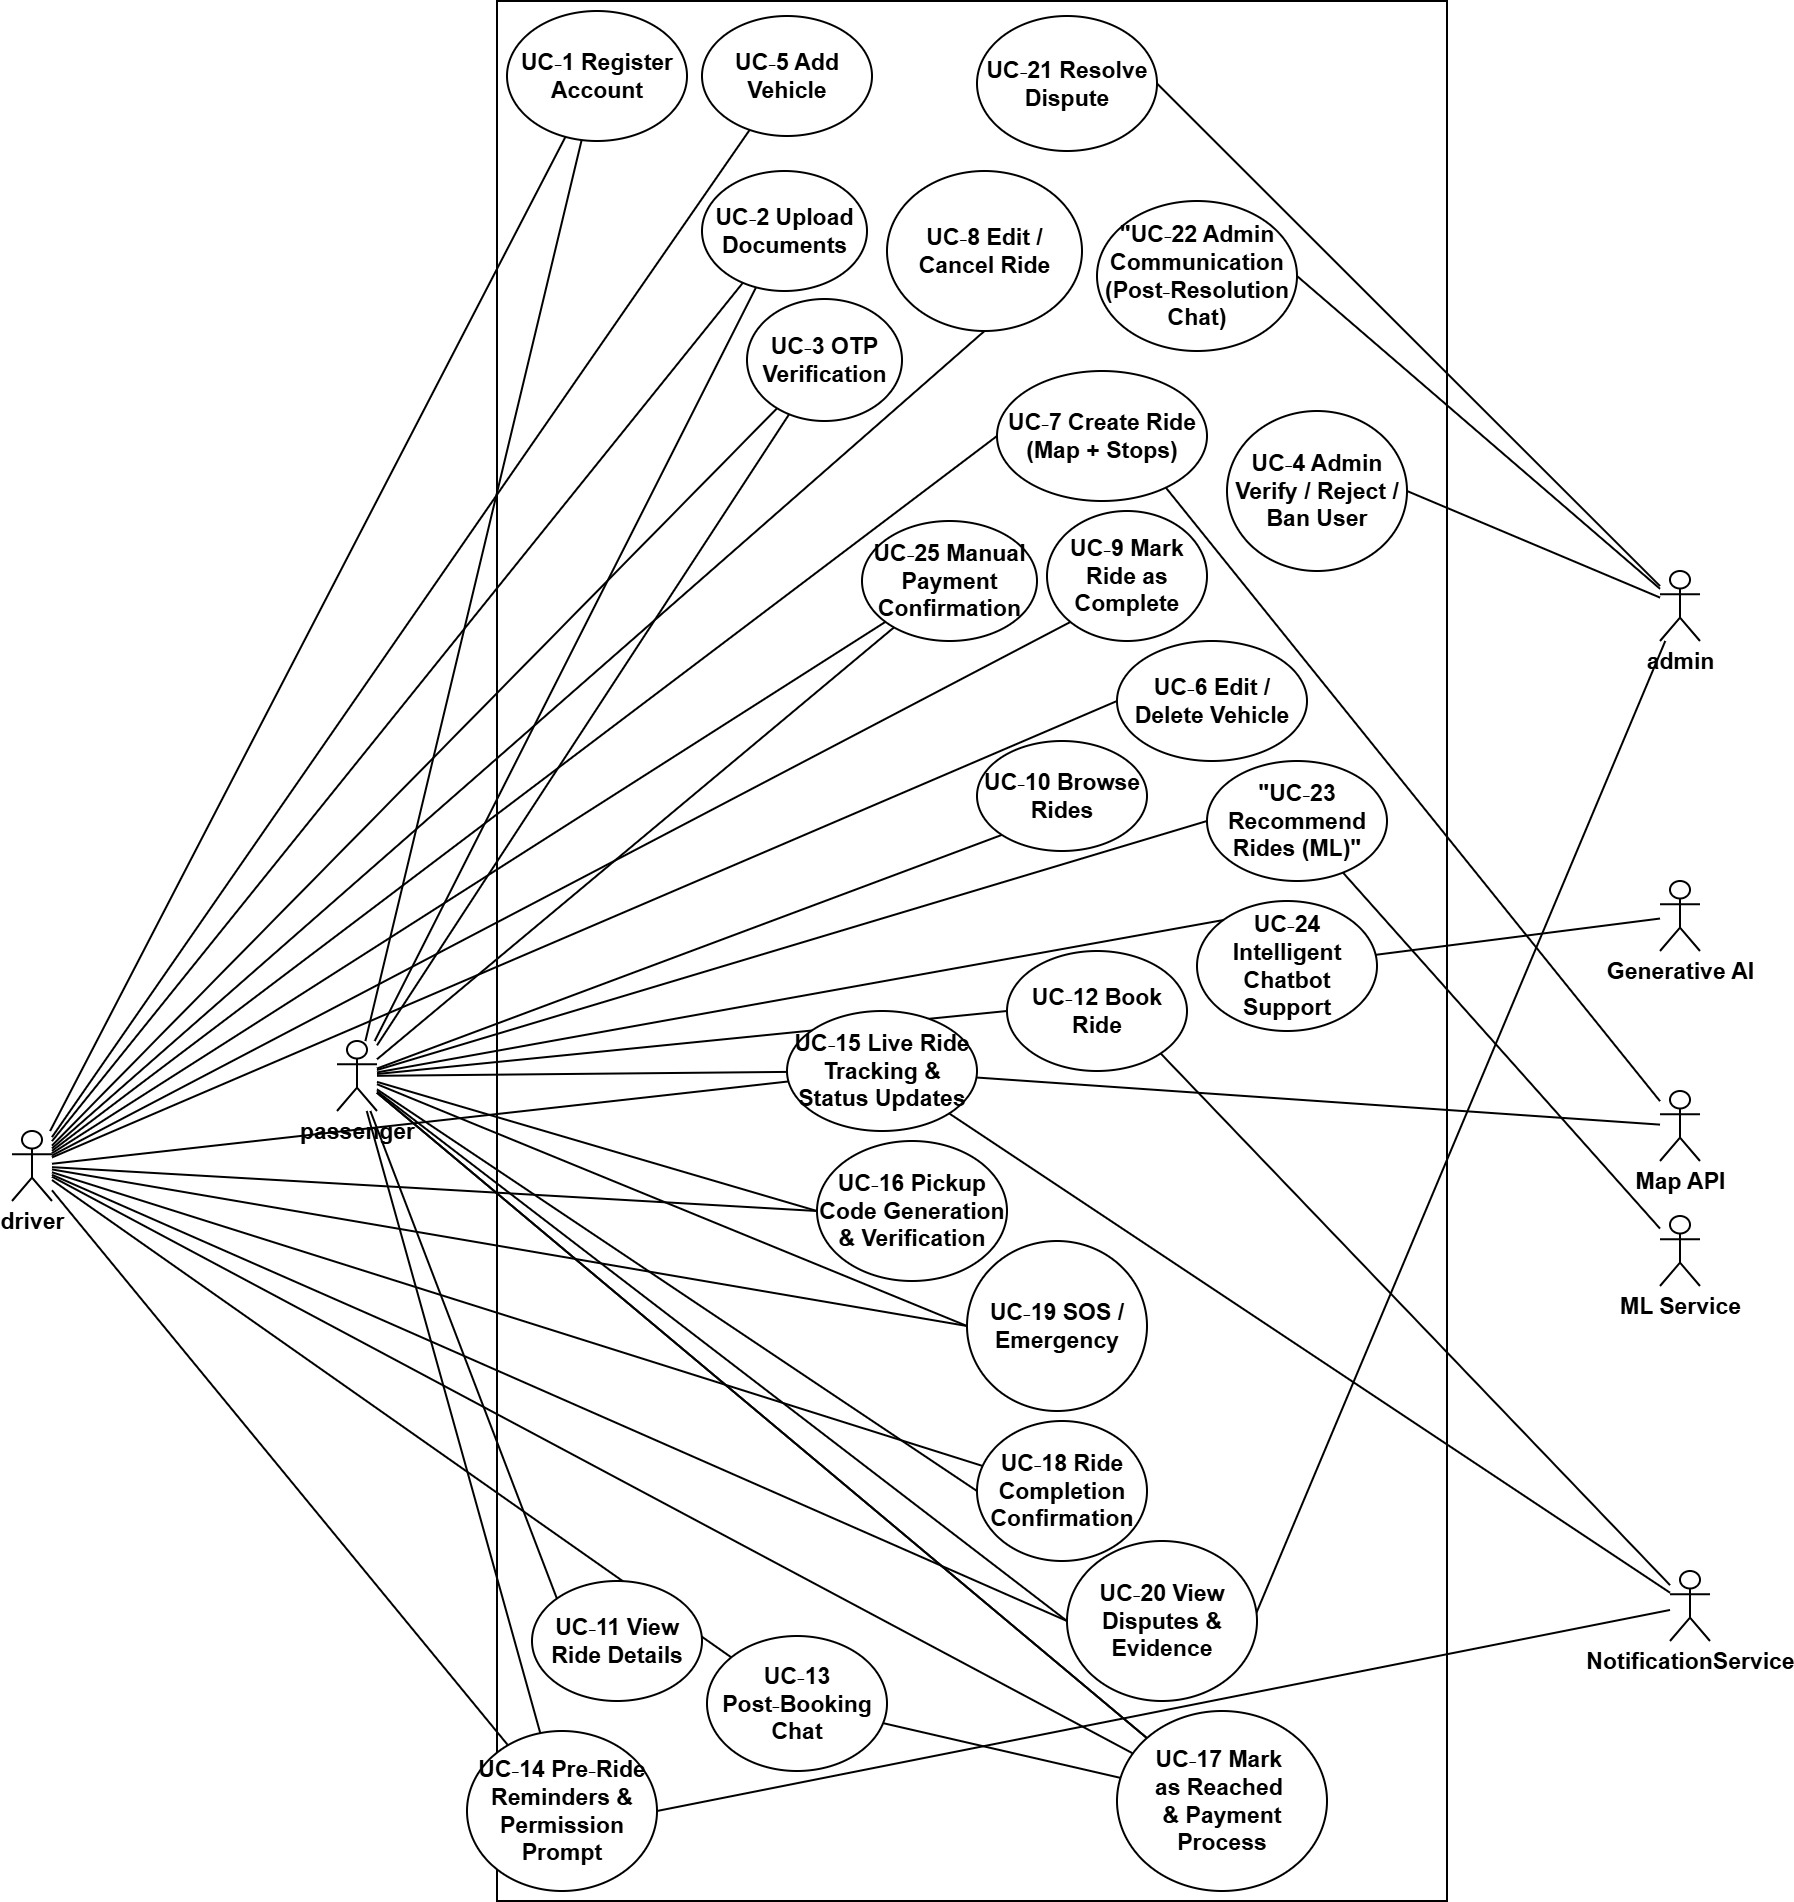
\includegraphics[width=\textwidth,keepaspectratio]{assets/master_uc.jpg}
    \caption{Master Use Case Diagram for the Lets Go Ride Sharing App system, covering all use cases and actor interactions.}
    \label{fig:master_uc}
\end{figure}

\begin{figure}[H]
    \centering
    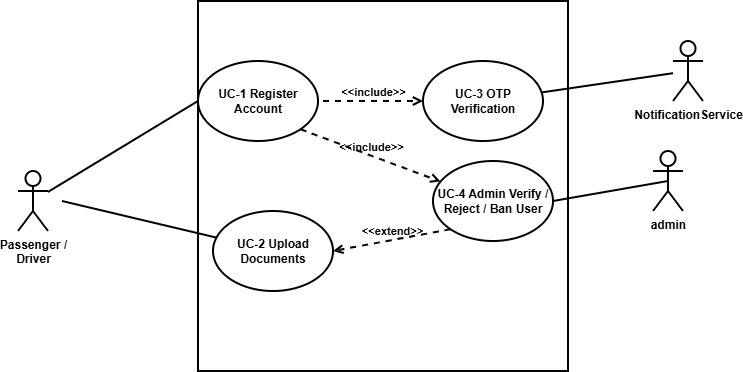
\includegraphics[width=0.8\textwidth,keepaspectratio,height=0.45\textheight]{assets/reg_verification_uc.jpg}
    \caption{Registration and Verification Theme: flow from account creation and multi-channel OTP verification to manual Admin identity approval.}
    \label{fig:registration_uc}
\end{figure}

\begin{figure}[H]
    \centering
    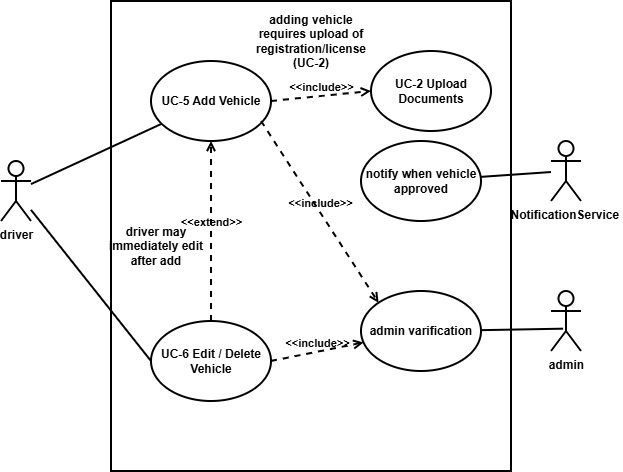
\includegraphics[width=0.8\textwidth,keepaspectratio,height=0.45\textheight]{assets/vehicle_management_uc.jpg}
    \caption{Vehicle Management: driver vehicle registration lifecycle and maintenance considerations.}
    \label{fig:vehicle_uc}
\end{figure}

\begin{figure}[H]
    \centering
    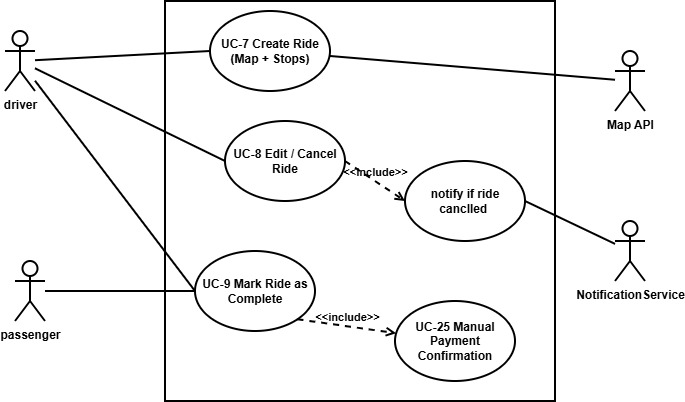
\includegraphics[width=0.8\textwidth,keepaspectratio,height=0.45\textheight]{assets/ride_management_uc.jpg}
    \caption{Ride Management: driver-side ride lifecycle from route creation to completion.}
    \label{fig:ride_mgmt_uc}
\end{figure}

\begin{figure}[H]
    \centering
    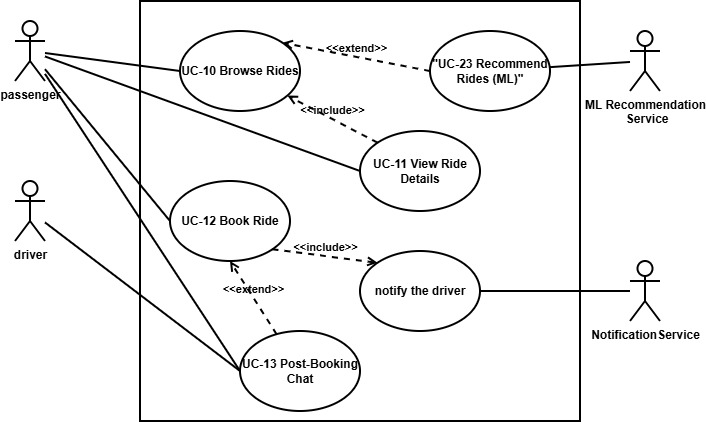
\includegraphics[width=0.8\textwidth,keepaspectratio,height=0.45\textheight]{assets/discovery_booking_uc.jpg}
    \caption{Discovery and Booking: passenger search, seat lock mechanism, and post-booking coordination.}
    \label{fig:booking_uc}
\end{figure}

\clearpage
\begin{figure}[H]
    \centering
    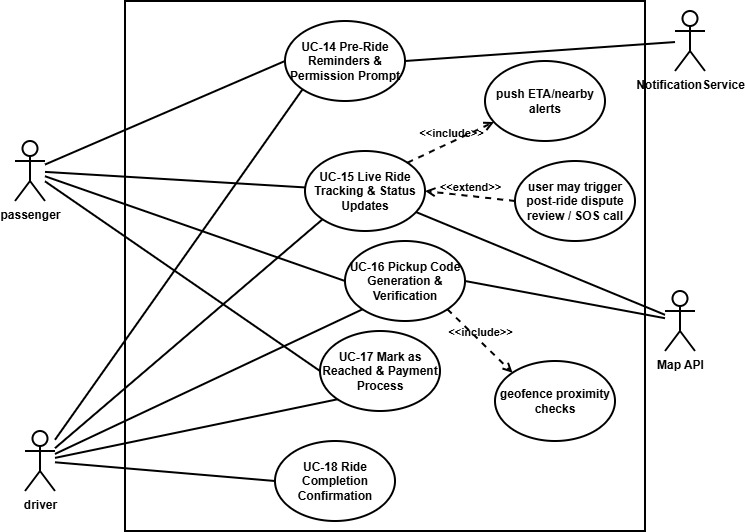
\includegraphics[width=0.8\textwidth,keepaspectratio,height=0.4\textheight]{assets/ride_execution_uc.jpg}
    \caption{Ride Execution Phase: live GPS tracking, geofenced pickup OTP verification, and arrival confirmations.}
    \label{fig:execution_uc}
\end{figure}

\begin{figure}[H]
    \centering
    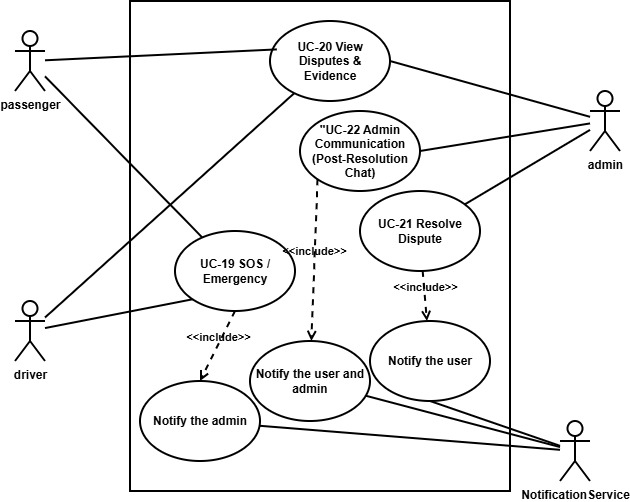
\includegraphics[width=0.8\textwidth,keepaspectratio,height=0.4\textheight]{assets/safety_disputes_uc.jpg}
    \caption{Safety and Disputes: SOS alerts, emergency escalation, and Admin audit workflows.}
    \label{fig:safety_uc}
\end{figure}

\clearpage
\begin{figure}[H]
    \centering
    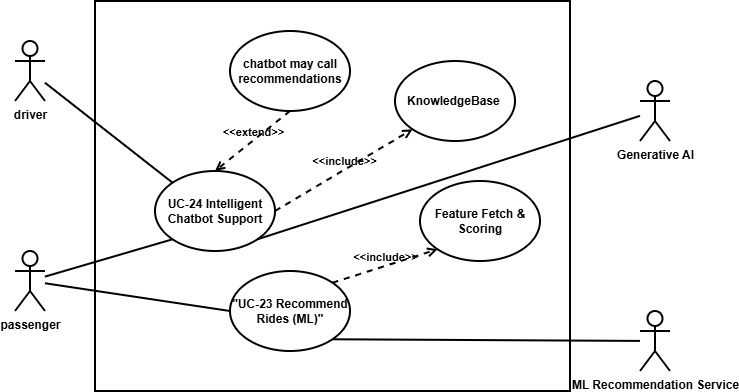
\includegraphics[width=0.8\textwidth,keepaspectratio,height=0.4\textheight]{assets/ml_chatbot_uc.jpg}
    \caption{AI/ML Features: content-based ride recommendations and generative AI support.}
    \label{fig:ai_uc}
\end{figure}

\begin{figure}[H]
    \centering
    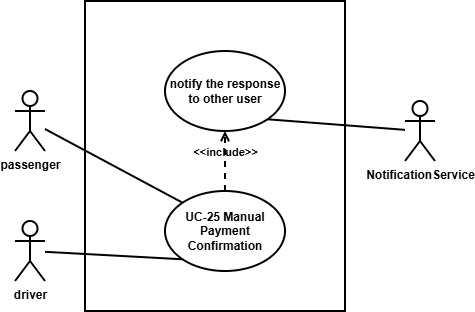
\includegraphics[width=0.8\textwidth,keepaspectratio,height=0.4\textheight]{assets/payment_uc.jpg}
    \caption{Manual Payment Flow: two-step verification for external transfers (Cash/Bank/QR).}
    \label{fig:payment_uc}
\end{figure}

\clearpage

%-----------------------------------------------------------------
\subsection{Use Case Descriptions}
%-----------------------------------------------------------------

This section provides detailed tabular specifications of all major use cases. These use cases form the basis for deriving functional requirements and are organised by thematic modules.

%============================================================================
\subsubsection{Registration \& Verification (UC-1 to UC-4)}
%============================================================================

% ============================================================================
% Use Case UC-1: Register Account
% ============================================================================
\begin{longtable}{|>{\raggedright\arraybackslash}p{4cm}|>{\raggedright\arraybackslash}p{11cm}|}
\caption{UC-1: Register Account}
\label{tab:uc-1} \\
\hline
\rowcolor{lightgray!30}
\textbf{Field} & \textbf{Value} \\
\hline
\endfirsthead
\hline
\rowcolor{lightgray!30}
\textbf{Field} & \textbf{Value} \\
\hline
\endhead
\hline
\endfoot
\hline
\endlastfoot
Use Case ID & UC-1 \\
\hline
Use Case Name & Register Account \\
\hline
Actors & \textbf{Primary Actor:} Unverified User \\
& \textbf{Secondary Actors:} Notification Service (email/SMS), Admin (implicit actor for later verification), Chatbot (optional help) \\
\hline
Description & An Unverified User registers a new account by supplying personal information and optional driver/bank details, uploads required documents (profile photo, live photo, CNIC front/back, driving license if applicable), receives OTPs via email and SMS, and completes OTP verification. Upon successful OTP verification the account transitions to \textit{Pending Admin Verification}. The use case guarantees collection of all data required for identification and enrollment. \\
\hline
Trigger & User launches the application and selects \textit{Create Account / Sign Up}. \\
\hline
Normal (Basic) Flow (Main Success Scenario) & 1. Unverified User opens the Registration screen and completes the registration form with required fields (name, username, email, password \& confirm password, address, phone number, CNIC, gender). \\
& 2. User may optionally provide bank account number and bank name (both required if one is supplied) and/or driving license number. \\
& 3. User uploads required documents (profile photo, live photo, CNIC front/back; driving license images if applicable; account QR if bank transfer desired). Client-side UI enforces format and size constraints before upload. \\
& 4. User submits the form; client performs basic checks (required fields, password strength) and a quick server uniqueness check for username/email. \\
& 5. Server validates inputs, creates a provisional user with status OTP\_VERIFICATION\_PENDING, and securely stores uploaded files. \\
& 6. System issues two OTPs (email and SMS/phone) with a 5-minute expiry and sends them via Notification Service. \\
& 7. User is prompted to enter both OTPs. \\
& 8. Server verifies OTPs; if both are valid and within expiry, the account state is set to PENDING\_ADMIN\_VERIFICATION and success is returned. \\
& 9. System displays a confirmation: ``OTP verified — your account is pending Admin verification. You will be notified on completion.'' \\
& 10. User is taken to login screen or offered to log in after Admin verification. \\
\hline
Preconditions & $\bullet$ User has a device with an active internet connection. \\
& $\bullet$ User has a valid email address and phone number to receive OTPs. \\
\hline
Postconditions & $\bullet$ \textbf{On success:} user account created with PENDING\_ADMIN\_VERIFICATION status and audit logs recorded. \\
& $\bullet$ \textbf{On failure:} user remains unverified; errors are reported to the user; provisional data retained per retention policy. \\
\hline
Alternate Flows \& Exceptions & \textbf{A1 — Missing Required Field / Client-side validation fails} \newline If the user omits required fields or client-side validation fails, display inline errors and block submission until corrected. Return to step 1. \\
& \textbf{A2 — Server-side validation failure (e.g., duplicate email/username)} \newline If server detects duplicate username/email or invalid CNIC format, return error to user with a clear message. User corrects input and resubmits. \\
& \textbf{A3 — Image upload fails (format/size or network error)} \newline Inform user which image failed and why (wrong format, too large or network issue). Allow retry and resume. \\
& \textbf{A4 — OTP expired / incorrect OTP} \newline If an OTP is expired or incorrect, display error and offer resend. Return to OTP entry step. \\
& \textbf{A5 — OTP delivery failure (SMS/email gateway problem)} \newline If Notification Service fails, show guidance (e.g., try alternate channel), log the failure, and increment monitoring metrics for Admin. \\
& \textbf{A6 — User abandons signup} \newline If user closes the app or session times out, provisional data is retained per retention policy. \\
\hline
Business Rules (BR) & \textbf{BR-1:} OTP expiration = 5 minutes. \\
& \textbf{BR-2:} If bank account number is entered, bank name is mandatory and vice versa. \\
& \textbf{BR-3:} Username and email must be unique. \\
& \textbf{BR-4:} Driving license images are required if driving license number is provided. \\
& \textbf{BR-5:} Limit OTP resend attempts to a configurable number (default: 3 per hour). \\
& \textbf{BR-6:} Uploaded images must satisfy configured size and format constraints; otherwise reject. \\
\hline
Assumptions & $\bullet$ Notification Service (email/SMS) is available and operational. \\
& $\bullet$ Users will have access to the email and phone provided for OTP reception. \\
& $\bullet$ CNIC format rules and validation logic are defined elsewhere and available to the system. \\
\end{longtable}

% ============================================================================
% Use Case UC-2: Upload Documents
% ============================================================================
\begin{longtable}{|>{\raggedright\arraybackslash}p{4cm}|>{\raggedright\arraybackslash}p{11cm}|}
\caption{UC-2: Upload Documents}
\label{tab:uc-2} \\
\hline
\rowcolor{lightgray!30}
\textbf{Field} & \textbf{Value} \\
\hline
\endfirsthead
\hline
\rowcolor{lightgray!30}
\textbf{Field} & \textbf{Value} \\
\hline
\endhead
\hline
\endfoot
\hline
\endlastfoot
Use Case ID & UC-2 \\
\hline
Use Case Name & Upload Documents \\
\hline
Actors & \textbf{Primary Actor:} Unverified User / User (during profile completion or driver onboarding) \\
& \textbf{Secondary Actors:} Notification Service (for confirmations), Admin (viewer during verification), Chatbot (optional help) \\
\hline
Description & A user uploads required identity and vehicle documents (profile photo, live photo, CNIC front/back, account QR, driving license front/back if applicable, and vehicle images when adding a vehicle). The system validates file formats and sizes, stores files securely, and associates them with the user or vehicle records. Uploaded documents are reviewed by Admins during verification. \\
\hline
Trigger & User navigates to the document-upload screen during registration, profile editing, or while adding a vehicle and initiates the upload action. \\
\hline
Normal (Basic) Flow (Main Success Scenario) & 1. User opens the Upload Documents section (during registration or via profile). \\
& 2. UI shows required and optional document slots with accepted formats and size limits (e.g., JPG/PNG, max dimensions/MB). \\
& 3. User selects a slot (e.g., CNIC front) and picks or captures an image. \\
& 4. Client performs light validation (file type, size) and shows immediate errors if invalid. \\
& 5. Client uploads files (multipart/form-data) including metadata (user\_id, document\_type, timestamp, optional vehicle\_id). \\
& 6. Server validates file type/signature, size, and dimensions, then stores the file securely. \\
& 7. Server creates a document record linking file location, document type, user\_id or vehicle\_id, upload timestamp and sets status to PENDING\_REVIEW. \\
& 8. Server returns success; UI displays thumbnail and status ``Uploaded — pending Admin review''. Notification Service may send confirmation. \\
& 9. Admin later reviews uploads in the Admin portal as part of verification flows. \\
\hline
Preconditions & $\bullet$ User is authenticated (in profile flow) or in registration flow with a stateful session. \\
& $\bullet$ Client device has camera or file access and internet connectivity. \\
\hline
Postconditions & $\bullet$ Document saved and linked to user/vehicle record. \\
& $\bullet$ Document status recorded (PENDING\_REVIEW / APPROVED / REJECTED). \\
& $\bullet$ Optional notification sent to user confirming upload. \\
\hline
Alternate Flows \& Exceptions & \textbf{A1 — Client-side Validation Failure (wrong format / too large)} \newline If client-side validation fails, show clear error and prevent upload; provide guidance on acceptable formats/sizes. Return to step 3. \\
& \textbf{A2 — Upload Interruption / Network Failure} \newline If upload fails mid-transfer, allow retry/resume where possible and retain a temporary local copy until success. Log failures. \\
& \textbf{A3 — Server-side Validation Failure (malformed file/signature mismatch)} \newline Server rejects the file with reason and prompts user to re-upload. \\
& \textbf{A4 — Duplicate or Previously Uploaded Document} \newline If a prior document of same type exists, UI shows both with timestamps and marks latest as current; replacement triggers re-verification per business rule. \\
& \textbf{A5 — Unauthorized Upload Attempt} \newline Unauthenticated/unauthorized uploads are rejected (401/403). \\
\hline
Business Rules (BR) & \textbf{BR-1:} Accepted file formats: JPG, PNG (configurable). \\
& \textbf{BR-2:} Max file size: 5 MB (configurable); reject larger files. \\
& \textbf{BR-3:} Driving license images required if license number is provided. \\
& \textbf{BR-4:} Account QR required if the user opts for bank-transfer payouts. \\
& \textbf{BR-5:} Replace/overwrite policy: uploading a new CNIC or license image sets status to PENDING\_REVIEW and triggers re-verification by Admin. \\
\hline
Assumptions & $\bullet$ Storage service is available. \\
& $\bullet$ Admins have a secure Admin portal to view/review documents. \\
\end{longtable}

% ============================================================================
% Use Case UC-3: OTP Verification
% ============================================================================
\begin{longtable}{|>{\raggedright\arraybackslash}p{4cm}|>{\raggedright\arraybackslash}p{11cm}|}
\caption{UC-3: OTP Verification}
\label{tab:uc-3} \\
\hline
\rowcolor{lightgray!30}
\textbf{Field} & \textbf{Value} \\
\hline
\endfirsthead
\hline
\rowcolor{lightgray!30}
\textbf{Field} & \textbf{Value} \\
\hline
\endhead
\hline
\endfoot
\hline
\endlastfoot
Use Case ID & UC-3 \\
\hline
Use Case Name & OTP Verification \\
\hline
Actors & \textbf{Primary Actor:} Unverified User (or User performing email/phone change) \\
& \textbf{Secondary Actors:} Notification Service (email/SMS), Admin (for logging/alerts), Chatbot (optional help) \\
\hline
Description & The system validates one-time passwords (OTPs) sent to a user's email and phone to confirm ownership of contact channels. Successful OTP verification transitions the account to PENDING\_ADMIN\_VERIFICATION. OTPs are short-lived (default 5 minutes) and subject to resend and attempt limits to prevent abuse. \\
\hline
Trigger & System sends OTPs after registration submission or when a user requests an email/phone change that requires re-verification; user navigates to the OTP entry screen. \\
\hline
Normal (Basic) Flow (Main Success Scenario) & 1. Following registration (UC-1) or contact-change request, the system generates an email OTP and an SMS OTP and sends them via Notification Service. \\
& 2. OTPs are stored securely with timestamps, expiry (default 5 minutes) and attempt counters. \\
& 3. User receives OTPs and opens the OTP entry screen. \\
& 4. User submits both OTP codes. \\
& 5. Server validates OTPs; if both are correct and within expiry, account state changes to PENDING\_ADMIN\_VERIFICATION and success is returned. \\
& 6. System shows a success message and redirects user to the appropriate screen (login or profile). \\
\hline
Preconditions & $\bullet$ User has completed the registration form or requested contact information change. \\
& $\bullet$ User has access to the provided email and phone for OTP reception. \\
& $\bullet$ Notification Service is operational. \\
\hline
Postconditions & $\bullet$ \textbf{On success:} User account state transitions to PENDING\_ADMIN\_VERIFICATION. \\
& $\bullet$ \textbf{On failure:} User remains in current state; OTP attempts are logged. \\
& $\bullet$ OTP verification event recorded in audit logs. \\
\hline
Alternate Flows \& Exceptions & \textbf{A1 — Wrong OTP Entered} \newline If user enters an incorrect OTP, display error with remaining attempts; user may retry within limits. \\
& \textbf{A2 — OTP Expired} \newline If OTP expires (default 5 minutes), inform user and offer resend. \\
& \textbf{A3 — Exceeded Attempt Limit} \newline If attempts exceed allowed limit (default 5), lock verification for a cooldown (default 15 minutes) and require support. \\
& \textbf{A4 — OTP Delivery Failure} \newline If Notification Service fails, log the failure, alert Admin, and provide alternate delivery options. \\
& \textbf{A5 — Resend OTP Requested} \newline On resend request, system issues new OTPs (invalidating prior ones) subject to resend limits. \\
& \textbf{A6 — User Cancels/Abandons} \newline If user leaves the OTP screen, OTPs remain until expiry; server may garbage-collect unused OTPs per retention policy. \\
\hline
Business Rules (BR) & \textbf{BR-1:} OTP expiry default = 5 minutes (Admin-configurable). \\
& \textbf{BR-2:} Max OTP verification attempts per OTP code = 5 (Admin-configurable); on exceed, impose cooldown (e.g., 15 minutes). \\
& \textbf{BR-3:} Max OTP resends per time window (e.g., 3 per hour) to avoid abuse. \\
& \textbf{BR-4:} OTPs are single-use; resending invalidates prior OTPs. \\
& \textbf{BR-5:} Avoid revealing which OTP channel failed; show generic ``OTP invalid'' with remaining attempts. \\
& \textbf{BR-6:} Record OTP generation and verification attempts for audit and fraud detection. \\
& \textbf{BR-7:} For contact-change workflows, require re-verification of the changed contact before applying the change. \\
\hline
Assumptions & $\bullet$ Users can access the email and phone they provide. \\
& $\bullet$ Time drift between server and client is negligible for 5-minute expiry; server time is authoritative. \\
& $\bullet$ Notification Service has reliable delivery mechanisms for email and SMS. \\
\end{longtable}

% ============================================================================
% Use Case UC-4: Admin Verify / Reject / Ban User
% ============================================================================
\begin{longtable}{|>{\raggedright\arraybackslash}p{4cm}|>{\raggedright\arraybackslash}p{11cm}|}
\caption{UC-4: Admin Verify / Reject / Ban User}
\label{tab:uc-4} \\
\hline
\rowcolor{lightgray!30}
\textbf{Field} & \textbf{Value} \\
\hline
\endfirsthead
\hline
\rowcolor{lightgray!30}
\textbf{Field} & \textbf{Value} \\
\hline
\endhead
\hline
\endfoot
\hline
\endlastfoot
Use Case ID & UC-4 \\
\hline
Use Case Name & Admin Verify / Reject / Ban User \\
\hline
Actors & \textbf{Primary Actor:} Admin \\
& \textbf{Secondary Actors:} User (awaiting verification), Notification Service (for sending approval/rejection messages) \\
\hline
Description & This use case defines how Admin reviews newly registered users and submitted documents, then chooses to verify, reject, or ban. Verification grants full access; rejection denies access with feedback and reapplication instructions; banning prevents future registrations with the same CNIC. Admins also handle disputes and can create accounts for special requests. \\
\hline
Trigger & Admin logs into the Admin portal and navigates to the User Verification section or receives an automated alert for new pending verifications. \\
\hline
Normal (Basic) Flow (Main Success Scenario) & 1. Admin opens the Admin Portal dashboard. \\
& 2. System lists users with status ``Pending Admin Verification.'' \\
& 3. Admin selects a user and views details: Name, Username, Email, Phone, CNIC, Gender, Address, and uploaded documents (profile photo, CNIC front/back, live photo, driving license). \\
& 4. Admin inspects documents for authenticity and completeness. \\
& 5. If acceptable, Admin selects ``Verify User'' and confirms. \\
& 6. System updates status from PENDING to VERIFIED. \\
& 7. Notification Service sends approval via email/SMS. \\
& 8. User receives full system access (login to dashboard). \\
\hline
Preconditions & $\bullet$ User has completed registration and OTP verification (UC-1, UC-3). \\
& $\bullet$ Admin is logged in with verification privileges. \\
& $\bullet$ Database and document storage are accessible. \\
\hline
Postconditions & $\bullet$ \textbf{On success:} User becomes active (verified) and can log in normally. \\
& $\bullet$ \textbf{On rejection:} User remains unverified; rejected status and reason recorded; user may reapply. \\
& $\bullet$ \textbf{On ban:} CNIC added to blacklist; login and registration disabled for that CNIC. \\
\hline
Alternate Flows \& Exceptions & \textbf{A1 — Rejection} \newline If Admin finds incomplete or inconsistent documents, they choose ``Reject User'' and provide a reason (e.g., ``Invalid CNIC''). System sets status to REJECTED and notifies user with reason. \\
& \textbf{A2 — Ban (Permanent Block)} \newline For confirmed fraud/unethical behaviour, Admin chooses ``Ban User'', confirms the action; system blacklists the CNIC, sets account to BANNED and notifies the user. \\
& \textbf{A3 — Dispute Resolution (Related Function)} \newline Admin reviews disputes in the Dispute Center, communicates with parties, and marks disputes Resolved or Escalated; system updates records accordingly. \\
& \textbf{A4 — Create Account (By Admin)} \newline Admin may create user accounts manually for support/test cases; such accounts can be created as Verified (bypassing OTP) per policy. \\
& \textbf{A5 — Verification Delay / Timeout} \newline Accounts without verification within 24 hours are flagged for Admin attention; system sends reminders or escalations per policy. \\
\hline
Business Rules (BR) & \textbf{BR-1:} Verification should occur within 24 hours of submission. \\
& \textbf{BR-2:} Only Admins with Verification Privilege may approve or reject users. \\
& \textbf{BR-3:} Banned CNICs cannot be re-registered. \\
& \textbf{BR-4:} All verification/rejection/ban actions must record Admin ID, timestamp and reason. \\
& \textbf{BR-5:} Notification Service should send decision messages within 2 minutes. \\
& \textbf{BR-6:} Admin cannot verify users missing mandatory documents. \\
& \textbf{BR-7:} Rejection retains the user record for audit and possible reapplication. \\
& \textbf{BR-8:} Verification changes are irreversible except by Super-Admin override. \\
\hline
Assumptions & $\bullet$ Admins are trained to identify fraudulent or edited documents. \\
& $\bullet$ Network and storage systems are stable so document previews load correctly. \\
& $\bullet$ Notification Service can reliably reach users (email/SMS). \\
\end{longtable}

%============================================================================
\subsubsection{Vehicle Management (UC-5 to UC-6)}
%============================================================================

% ============================================================================
% Use Case UC-5: Add Vehicle
% ============================================================================
\begin{longtable}{|>{\raggedright\arraybackslash}p{4cm}|>{\raggedright\arraybackslash}p{11cm}|}
\caption{UC-5: Add Vehicle}
\label{tab:uc-5} \\
\hline
\rowcolor{lightgray!30}
\textbf{Field} & \textbf{Value} \\
\hline
\endfirsthead
\hline
\rowcolor{lightgray!30}
\textbf{Field} & \textbf{Value} \\
\hline
\endhead
\hline
\endfoot
\hline
\endlastfoot
Use Case ID & UC-5 \\
\hline
Use Case Name & Add Vehicle \\
\hline
Actors & \textbf{Primary Actor:} Verified Driver \\
& \textbf{Secondary Actors:} Map/Routing Service, Notification Service, ML Service (for indexing) \\
\hline
Description & A verified Driver registers a vehicle by providing required vehicle details (model, variant, company, plate number, type, color, seats, engine/chassis optional, fuel type, registration/insurance optional, and vehicle images). The system validates inputs, stores vehicle metadata, and links the vehicle to the driver account. Vehicle verification may be required by Admin per policy. \\
\hline
Trigger & Driver navigates to Profile $\rightarrow$ Vehicles and taps Add Vehicle. \\
\hline
Normal (Basic) Flow (Main Success Scenario) & 1. Driver opens Profile $\rightarrow$ Vehicles and taps Add Vehicle. \\
& 2. System displays a form with required fields: vehicle model, company, variant, plate number, type (2W/4W), color, number of seats, fuel type, and optional engine/chassis numbers. \\
& 3. Driver fills in vehicle details; client validates format and required fields. \\
& 4. Driver uploads vehicle images (front, back, documents) with client-side format/size validation. \\
& 5. Driver submits the form. \\
& 6. Server validates inputs, checks plate uniqueness, validates image sizes/formats, and stores vehicle record linked to driver account. \\
& 7. Vehicle status set to VERIFIED (or PENDING\_REVIEW if policy requires Admin approval for critical fields). \\
& 8. System displays success message; vehicle appears in driver's vehicle list and becomes available for ride creation. \\
\hline
Preconditions & $\bullet$ Driver is authenticated and verified. \\
& $\bullet$ Driver has completed registration including document upload. \\
\hline
Postconditions & $\bullet$ \textbf{On success:} Vehicle record created and linked to driver account; vehicle available for ride creation. \\
& $\bullet$ \textbf{On failure:} User shown error; vehicle not saved; client retains form data for retry. \\
\hline
Alternate Flows \& Exceptions & \textbf{AF-1 — Validation Failure (required field missing / invalid format)} \newline If validation fails (missing model, invalid plate format), display inline errors and block submission. \\
& \textbf{AF-2 — Image Upload Failure} \newline If image size or format invalid, show error and allow retry. \\
& \textbf{AF-3 — Duplicate Plate Number} \newline If plate number already registered to another user, reject and show error; driver corrects and resubmits. \\
& \textbf{AF-4 — Vehicle Type Mismatch} \newline If driver selects 2W but enters seat count $\neq$ 2, show warning and auto-correct seats to 2. \\
& \textbf{AF-5 — Admin Review Required} \newline If vehicle record requires Admin approval per policy, system sets status to PENDING\_REVIEW and notifies driver to wait for verification. \\
\hline
Business Rules (BR) & \textbf{BR-1:} 2W vehicles must have seat count = 2 (system-enforced). \\
& \textbf{BR-2:} 4W vehicles can have 4–7 seats (configurable); system enforces min/max. \\
& \textbf{BR-3:} Plate number must be unique across all vehicles in the system. \\
& \textbf{BR-4:} Vehicle images must be valid format (JPG/PNG) and less than 1 MB. \\
& \textbf{BR-5:} Optional fields (insurance expiry, engine/chassis) may be added or edited later. \\
\hline
Assumptions & $\bullet$ Driver is familiar with vehicle registration details. \\
& $\bullet$ Plate numbers provided are correct and unique. \\
& $\bullet$ Storage service available for vehicle images. \\
\end{longtable}

% ============================================================================
% Use Case UC-6: Edit / Delete Vehicle
% ============================================================================
\begin{longtable}{|>{\raggedright\arraybackslash}p{4cm}|>{\raggedright\arraybackslash}p{11cm}|}
\caption{UC-6: Edit / Delete Vehicle}
\label{tab:uc-6} \\
\hline
\rowcolor{lightgray!30}
\textbf{Field} & \textbf{Value} \\
\hline
\endfirsthead
\hline
\rowcolor{lightgray!30}
\textbf{Field} & \textbf{Value} \\
\hline
\endhead
\hline
\endfoot
\hline
\endlastfoot
Use Case ID & UC-6 \\
\hline
Use Case Name & Edit / Delete Vehicle \\
\hline
Actors & \textbf{Primary Actor:} Driver (verified, with vehicle(s) registered) \\
& \textbf{Secondary Actors:} Admin (may be required for approvals), Notification Service (in-app/email confirmations) \\
\hline
Description & A verified Driver may edit details of an existing vehicle (for example color, insurance expiry, or permitted seat changes for 4W) or request deletion. The system validates edits, applies business rules, may set the vehicle to PENDING\_REVIEW for Admin approval for critical changes, and prevents deletion if the vehicle is linked to active or scheduled rides unless policy allows. \\
\hline
Trigger & Driver selects a vehicle from their profile listing and chooses Edit or Delete. \\
\hline
Normal (Basic) Flow --- Edit Vehicle & 1. Driver opens Profile $\rightarrow$ Vehicles and selects a vehicle. \\
& 2. Driver clicks Edit; the system presents current details in an editable form. \\
& 3. Driver modifies allowed fields (color, insurance expiry, engine/chassis if permitted, number of seats for 4W). \\
& 4. Client validates constraints and submits changes. \\
& 5. Server enforces business rules (e.g., 2W seats fixed=2, plate uniqueness). \\
& 6. If non-critical, server updates record, logs the change, and returns success. \\
& 7. If critical (plate, registration) or policy requires, server sets status to PENDING\_REVIEW and notifies Admin. \\
\hline
Normal (Basic) Flow --- Delete Vehicle & 1. Driver selects Delete; system shows confirmation. \\
& 2. Driver confirms. \\
& 3. Server checks dependencies (active/future rides). If dependencies exist, block deletion and report affected rides; otherwise perform a soft delete and return success. \\
\hline
Preconditions & $\bullet$ Driver is authenticated and owns the vehicle. \\
& $\bullet$ Vehicle record exists and is accessible. \\
\hline
Postconditions & $\bullet$ \textbf{On successful edit:} vehicle updated and audit logged; possibly set to PENDING\_REVIEW. \\
& $\bullet$ \textbf{On successful delete:} vehicle marked deleted and removed from selection lists; historical references preserved. \\
\hline
Alternate Flows \& Exceptions & \textbf{A1 — Validation Error on Edit} \newline If server-side validation fails (invalid plate, seats not allowed, duplicate plate), return error and do not persist changes. \\
& \textbf{A2 — Edit Requiring Admin Approval} \newline If critical fields are changed, set status to PENDING\_REVIEW and restrict usage until review completes. \\
& \textbf{A3 — Attempt to Delete Vehicle with Active/Future Rides} \newline Block deletion and show affected rides. \\
& \textbf{A4 — Unauthorized Action} \newline Reject unauthorised edit/delete attempts (401/403). \\
\hline
Business Rules (BR) & \textbf{BR-1:} Only the vehicle owner or Admin may edit/delete vehicle records. \\
& \textbf{BR-2:} 2W vehicles must have seats fixed to 2. \\
& \textbf{BR-3:} Plate number changes may trigger PENDING\_REVIEW and require Admin approval. \\
& \textbf{BR-4:} Vehicles tied to active or future rides cannot be deleted unless policy allows. \\
\hline
Assumptions & $\bullet$ Admin review workflow (if enabled) is available. \\
& $\bullet$ Vehicle-ride relationships are enforced to prevent accidental deletion. \\
\end{longtable}

%============================================================================
\subsubsection{Ride Management (UC-7 to UC-9)}
%============================================================================

% ============================================================================
% Use Case UC-7: Create Ride (map + stops)
% ============================================================================
\begin{longtable}{|>{\raggedright\arraybackslash}p{4cm}|>{\raggedright\arraybackslash}p{11cm}|}
\caption{UC-7: Create Ride (map + stops)}
\label{tab:uc-7} \\
\hline
\rowcolor{lightgray!30}
\textbf{Field} & \textbf{Value} \\
\hline
\endfirsthead
\hline
\rowcolor{lightgray!30}
\textbf{Field} & \textbf{Value} \\
\hline
\endhead
\hline
\endfoot
\hline
\endlastfoot
Use Case ID & UC-7 \\
\hline
Use Case Name & Create Ride (map + stops) \\
\hline
Actors & \textbf{Primary Actor:} Driver \\
& \textbf{Secondary Actors:} Map/Routing Service, Notification Service, ML Service (for indexing) \\
\hline
Description & A verified Driver creates a new ride listing by defining a route on a map (start, intermediate, and end stops), selecting a vehicle, setting ride parameters (date/time, seats, gender preference, fare), and publishing it. The system validates the route, calculates fare, and makes the ride discoverable to passengers. \\
\hline
Trigger & Driver navigates to Create Ride screen from the driver dashboard. \\
\hline
Normal (Basic) Flow (Main Success Scenario) & 1. Driver opens Create Ride $\rightarrow$ map view opens centered on their current location (or last used area). \\
& 2. Driver marks the route: tap to add start stop, then intermediate stops, and an end stop. UI shows start (green), intermediates (orange), end (red) the system connects these stops with polylines and suggests a sample route. \\
& 3. For each stop the system fetches a suggested place name from map provider (autofill); the driver may accept or edit the stop name inline. Driver may re-order stops or delete a stop. \\
& 4. Driver uses the search bar (free-text) to find/insert known places or addresses if desired. \\
& 5. Driver selects a registered vehicle for the ride from a modal list (vehicle metadata preview shown). If no vehicle exists, the UI prompts the driver to add a vehicle (link to UC-5). The driver confirms vehicle selection. \\
& 6. Driver provides ride parameters: Date \& departure time, Available seats (system reserves 1 seat for driver), Gender preference (All / Male Only / Female Only), Allow fare negotiation?, Base/total fare (system displays auto-calculated fare, driver may edit whole-route fare or per-stop pricing), Optional description/rules. \\
& 7. System performs validations (see Business Rules) and computes: Route polyline + distance (km), Estimated duration (minutes), Default fare per seat and total fare, Estimated per-stop fares. \\
& 8. Driver previews ride summary (map, stops, date/time, seats, fare, vehicle). \\
& 9. Driver clicks Create Ride / Publish. System persists ride with status PUBLISHED (or PENDING if Admin/vehicle review required). \\
& 10. System adds rides to My Rides (driver view) and to passenger discovery feeds per ML Service. \\
& 11. If any post-creation background actions apply (e.g., route indexing, ML indexing), the system queues them and marks the ride fully available when indexing finishes. \\
\hline
Preconditions & $\bullet$ Driver is authenticated and Verified (FR-2 / FR-14), or driver has license number present per policy. \\
& $\bullet$ Driver has at least one registered vehicle available (FR-3). \\
& $\bullet$ Map and routing service available (online). \\
& $\bullet$ Driver is not blocked from creating rides by Admin sanctions. \\
\hline
Postconditions & $\bullet$ \textbf{On success:} Ride record saved (route polyline, stops, metadata), Ride appears in driver's My Rides list with status CREATED or PUBLISHED, Ride is discoverable by passengers. \\
\hline
Alternate Flows \& Exceptions & \textbf{AF-1 — Missing required fields / validation fails} \newline If driver fails validations (date in past, no vehicle selected, seats = 0, less than two stops), show inline errors and block publishing until corrected. \\
& \textbf{AF-2 — Low-quality or incomplete route} \newline If route is illogical (very short distance, reverse ordering) system warns and suggests corrections; driver can confirm override if allowed by policy. \\
& \textbf{AF-3 — Vehicle not verified or suspended} \newline If selected vehicle is PENDING\_REVIEW or SUSPENDED, UI warns driver and either blocks publishing or allows publishing depending on policy. If blocked, prompt to choose another vehicle or contact Admin. \\
& \textbf{AF-4 — Driver has an active in-progress ride} \newline Per policy, driver is allowed to create a new ride listing even if they have an active ride but cannot start a different in-progress ride (FR-16.6). Show a note reminding drivers they cannot start another active ride until current ride completed. \\
& \textbf{AF-5 — Edits after passengers booked} \newline If driver attempts to edit a published ride that already has confirmed bookings, system does not allow alternative actions (cancel ride or contact passengers). \\
& \textbf{AF-6 — Network / Map service fails} \newline If routing/map provider fails, allow driver to save a draft ride with basic data (start, end, textual stops) and queue a background job to compute route when service is available. Indicate draft status in UI. \\
\hline
Business Rules (BR) & \textbf{BR-1:} Driver seat reserved: available passenger seats = vehicle seats − 1 (enforced). \\
& \textbf{BR-2:} Departure date/time must be in the future. \\
& \textbf{BR-3:} Minimum stops: at least a start and an end (>=2 stops). \\
& \textbf{BR-4:} If driver enables negotiation, negotiation flags stored in ride metadata and passenger negotiation UI enabled. \\
& \textbf{BR-5:} Auto-fare calculation uses distance $\times$ vehicle\_rate + base\_fee; driver may override but must confirm when overriding auto fare. Formula is configurable in Admin settings. \\
& \textbf{BR-6:} Edits to route, seat counts, or fare are blocked if confirmed bookings exist (unless driver cancels ride). \\
& \textbf{BR-7:} If vehicle is multi-seat (4W), driver can set passenger seat split by gender preference; UI must enforce gender-based avail seats. \\
& \textbf{BR-8:} Ride status lifecycle: DRAFT $\rightarrow$ PUBLISHED $\rightarrow$ IN\_PROGRESS $\rightarrow$ COMPLETED $\rightarrow$ ARCHIVED. Publishing sets visible to passengers and driver. \\
\hline
Assumptions & $\bullet$ Map/routing provider (e.g., Google/OSM) is available and returns reliable place names, polylines, distance and duration. \\
& $\bullet$ Driver understands the effect of reserving one seat for themselves. \\
& $\bullet$ Admin-configurable rules (max stops, auto-fare formula, review policy) exist and are set before go-live. \\
\end{longtable}

% ============================================================================
% Use Case UC-8: Edit / Cancel Ride
% ============================================================================
\begin{longtable}{|>{\raggedright\arraybackslash}p{4cm}|>{\raggedright\arraybackslash}p{11cm}|}
\caption{UC-8: Edit / Cancel Ride}
\label{tab:uc-8} \\
\hline
\rowcolor{lightgray!30}
\textbf{Field} & \textbf{Value} \\
\hline
\endfirsthead
\hline
\rowcolor{lightgray!30}
\textbf{Field} & \textbf{Value} \\
\hline
\endhead
\hline
\endfoot
\hline
\endlastfoot
Use Case ID & UC-8 \\
\hline
Use Case Name & Edit / Cancel Ride \\
\hline
Actors & \textbf{Primary Actor:} Driver \\
& \textbf{Secondary Actors:} Passenger(s), Notification Service, Admin \\
\hline
Description & Driver may edit a published ride (when permitted by policy) or cancel a ride. The system enforces edit restrictions when confirmed bookings exist and notifies affected passengers on cancellation. \\
\hline
Trigger & Driver selects a ride from My Rides and chooses Edit or Cancel. \\
\hline
Normal (Basic) Flow (Main Success Scenario) & 1. Driver opens My Rides and selects a ride. \\
& 2. If Edit is chosen, the system displays editable fields and validates changes before saving. \\
& 3. If Cancel is chosen, the system requests a reason and asks for confirmation. \\
& 4. On confirmation, the system updates ride status to CANCELLED and notifies affected passengers. \\
\hline
Preconditions & $\bullet$ Driver is authenticated and is the owner of the ride. \\
& $\bullet$ Ride is in a state that allows editing/cancellation per policy. \\
\hline
Postconditions & $\bullet$ Ride is updated or cancelled; audit logs recorded; notifications dispatched as applicable. \\
\hline
Alternate Flows \& Exceptions & \textbf{AF-1 — Edit blocked due to confirmed bookings} \newline If confirmed bookings exist and policy forbids edits, prevent save and suggest cancellation. \\
& \textbf{AF-2 — Cancellation while IN\_PROGRESS} \newline If ride is IN\_PROGRESS and driver cancels, send high-priority notifications and escalate per safety procedures. \\
\hline
Business Rules (BR) & \textbf{BR-1:} Editing rules are policy-based and may be restricted once bookings exist. \\
& \textbf{BR-2:} Cancellation actions must be logged with timestamp and reason. \\
\hline
Assumptions & $\bullet$ Notification Service is available for timely updates. \\
\end{longtable}

% ============================================================================
% Use Case UC-9: Mark Ride as Complete
% ============================================================================
\begin{longtable}{|>{\raggedright\arraybackslash}p{4cm}|>{\raggedright\arraybackslash}p{11cm}|}
\caption{UC-9: Mark Ride as Complete}
\label{tab:uc-9} \\
\hline
\rowcolor{lightgray!30}
\textbf{Field} & \textbf{Value} \\
\hline
\endfirsthead
\hline
\rowcolor{lightgray!30}
\textbf{Field} & \textbf{Value} \\
\hline
\endhead
\hline
\endfoot
\hline
\endlastfoot
Use Case ID & UC-9 \\
\hline
Use Case Name & Mark Ride as Complete \\
\hline
Actors & \textbf{Primary Actor:} Driver \\
& \textbf{Secondary Actors:} Passenger(s), Notification Service, Admin \\
\hline
Description & At trip end the Driver marks the ride as complete. The system finalizes ride state, records completion timestamp, triggers notifications, and enables rating and feedback workflows. \\
\hline
Trigger & Driver selects Mark Ride as Complete in the driver app. \\
\hline
Normal (Basic) Flow (Main Success Scenario) & 1. Driver reaches the final destination. \\
& 2. Driver taps Mark Ride as Complete. \\
& 3. System validates ride state (must be IN\_PROGRESS) and records completion timestamp. \\
& 4. System notifies passengers and opens rating/feedback prompts. \\
\hline
Preconditions & $\bullet$ Ride status is IN\_PROGRESS. \\
\hline
Postconditions & $\bullet$ Ride status becomes COMPLETED and completion event is recorded in audit logs. \\
\hline
Alternate Flows \& Exceptions & \textbf{AF-1 — Completion blocked by active dispute/SOS} \newline If an active dispute or SOS exists, block completion until resolution. \\
\hline
Business Rules (BR) & \textbf{BR-1:} Completion events are auditable and retained per policy. \\
\hline
Assumptions & $\bullet$ Required network connectivity is available to submit completion. \\
\end{longtable}

% ============================================================================
% Use Case UC-10: Browse Rides
% ============================================================================
\begin{longtable}{|>{\raggedright\arraybackslash}p{4cm}|>{\raggedright\arraybackslash}p{11cm}|}
\caption{UC-10: Browse Rides}
\label{tab:uc-10} \\
\hline
\rowcolor{lightgray!30}
\textbf{Field} & \textbf{Value} \\
\hline
\endfirsthead
\hline
\rowcolor{lightgray!30}
\textbf{Field} & \textbf{Value} \\
\hline
\endhead
\hline
\endfoot
\hline
\endlastfoot
Use Case ID & UC-10 \\
\hline
Use Case Name & Browse Rides \\
\hline
Actors & \textbf{Primary Actor:} Passenger \\
& \textbf{Secondary Actors:} ML Service (for ranking), Map Service, Notification Service \\
\hline
Description & A verified Passenger searches and browses available rides using filters (origin/destination, date/time, gender preference, price, vehicle type, negotiation). The system returns ride cards with key information and options to view details or book. \\
\hline
Trigger & Passenger opens the Browse Rides screen. \\
\hline
Normal (Basic) Flow (Main Success Scenario) & 1. Passenger opens Browse Rides and sees a default list (e.g., recommended rides and a search box). \\
& 2. Passenger enters search criteria or applies filters. \\
& 3. System queries the ride index and returns matching rides sorted by relevance/ranking. \\
& 4. Passenger selects a ride to view details (UC-11) or taps Book to begin UC-12. \\
\hline
Preconditions & $\bullet$ Passenger is authenticated and verified. \\
& $\bullet$ The system has active published rides. \\
& $\bullet$ Internet connection and map/search services are available. \\
\hline
Postconditions & $\bullet$ Passenger sees matching rides and can proceed to UC-11 or UC-12. \\
& $\bullet$ Search activity may be logged for analytics/personalization. \\
\hline
Alternate Flows \& Exceptions & \textbf{AF-1 — No matches found} \newline Show ``No rides found'' and suggest adjusting filters or pickup area. \\
& \textbf{AF-2 — Map unavailable} \newline Fall back to a textual list view if map tiles fail. \\
\hline
Business Rules (BR) & \textbf{BR-1:} Only PUBLISHED rides with departure times in the future are shown. \\
& \textbf{BR-2:} Ride cards do not expose passenger PII; contact details are hidden prior to confirmation. \\
\hline
Assumptions & $\bullet$ Search/index data is available and refreshed periodically. \\
\end{longtable}

% ============================================================================
% Use Case UC-11: View Ride Details
% ============================================================================
\begin{longtable}{|>{\raggedright\arraybackslash}p{4cm}|>{\raggedright\arraybackslash}p{11cm}|}
\caption{UC-11: View Ride Details}
\label{tab:uc-11} \\
\hline
\rowcolor{lightgray!30}
\textbf{Field} & \textbf{Value} \\
\hline
\endfirsthead
\hline
\rowcolor{lightgray!30}
\textbf{Field} & \textbf{Value} \\
\hline
\endhead
\hline
\endfoot
\hline
\endlastfoot
Use Case ID & UC-11 \\
\hline
Use Case Name & View Ride Details \\
\hline
Actors & \textbf{Primary Actor:} Passenger (verified user) \\
& \textbf{Secondary Actors:} Notification Service, ML Service (optional) \\
\hline
Description & When a passenger selects a ride card they see full ride information: route and stops, date/time, driver profile, vehicle details, fare breakdown, gender preference, seat availability and driver rules. From here they may proceed to booking (UC-12) or save/share the ride. \\
\hline
Trigger & Passenger taps a ride from the Browse Rides list (UC-10). \\
\hline
Normal (Basic) Flow (Main Success Scenario) & 1. Passenger selects a ride card. \\
& 2. System fetches and displays detailed ride information with a map preview and action buttons (Book/Save/Share; Negotiate if enabled). \\
& 3. Passenger proceeds to UC-12 to book if desired. \\
\hline
Preconditions & $\bullet$ Passenger is authenticated and verified. \\
& $\bullet$ Ride exists and is PUBLISHED with a future departure time. \\
\hline
Postconditions & $\bullet$ Passenger views ride details and can proceed to booking or save/share the ride. \\
\hline
Alternate Flows \& Exceptions & \textbf{AF-1 — Ride no longer available} \newline If the ride is cancelled/expired/full, show a message and suggest alternatives. \\
& \textbf{AF-2 — Network failure} \newline If fetching details fails, display an error and allow retry. \\
\hline
Business Rules (BR) & \textbf{BR-1:} Driver contact details are withheld until booking is confirmed. \\
& \textbf{BR-2:} Gender preference rules are shown clearly and enforced during booking. \\
\hline
Assumptions & $\bullet$ Passenger device can render a map preview or a fallback view. \\
\end{longtable}

% ============================================================================
% Use Case UC-12: Book Ride (select seats / pickup & drop)
% ============================================================================
\begin{longtable}{|>{\raggedright\arraybackslash}p{4cm}|>{\raggedright\arraybackslash}p{11cm}|}
\caption{UC-12: Book Ride (select seats / pickup \& drop)}
\label{tab:uc-12} \\
\hline
\rowcolor{lightgray!30}
\textbf{Field} & \textbf{Value} \\
\hline
\endfirsthead
\hline
\rowcolor{lightgray!30}
\textbf{Field} & \textbf{Value} \\
\hline
\endhead
\hline
\endfoot
\hline
\endlastfoot
Use Case ID & UC-12 \\
\hline
Use Case Name & Book Ride (select seats / pickup \& drop) \\
\hline
Actors & \textbf{Primary Actor:} Passenger (verified) \\
& \textbf{Secondary Actors:} Driver, Notification Service, Admin (for escalations/disputes) \\
\hline
Description & Passenger books one or more seats on a published ride by selecting pickup and drop stops from the driver route, choosing seat count (and gender split if applicable), confirming fare/payment preference, and submitting a booking request. The system verifies availability, records the booking, and notifies the driver to accept or reject. \\
\hline
Trigger & Passenger taps Book Ride from Ride Details (UC-11). \\
\hline
Normal (Basic) Flow (Main Success Scenario) & 1. Passenger selects pickup and drop stops from the driver's route. \\
& 2. Passenger selects seat count; UI enforces any gender-preference constraints. \\
& 3. System calculates fare for the selected segment and displays a breakdown. \\
& 4. Passenger submits the booking request. \\
& 5. System creates a booking with status REQUESTED and notifies the driver. \\
& 6. Driver accepts or rejects; on accept booking moves to CONFIRMED and passenger is notified. \\
\hline
Preconditions & $\bullet$ Passenger is authenticated and verified. \\
& $\bullet$ Ride is PUBLISHED and has available seats. \\
\hline
Postconditions & $\bullet$ Booking recorded and transitions to CONFIRMED or REJECTED. \\
& $\bullet$ Notifications are sent to driver and passenger. \\
\hline
Alternate Flows \& Exceptions & \textbf{AF-1 — Seats no longer available} \newline If availability changes before confirmation, reject the request and prompt passenger to retry. \\
& \textbf{AF-2 — Driver does not respond} \newline If driver does not respond within the configured window, booking expires/cancels per policy and passenger is notified. \\
\hline
Business Rules (BR) & \textbf{BR-1:} Seat reservation/lock window is configurable; seats release on expiry. \\
& \textbf{BR-2:} Driver contact details are shared only after booking is confirmed (policy-based). \\
\hline
Assumptions & $\bullet$ Payment method selection and manual payment evidence flow follow FR-13 policies. \\
\end{longtable}

% ============================================================================
% Use Case UC-13: Post-Booking Chat (1:1 & Broadcast)
% ============================================================================
\begin{longtable}{|>{\raggedright\arraybackslash}p{4cm}|>{\raggedright\arraybackslash}p{11cm}|}
\caption{UC-13: Post-Booking Chat (1:1 \& Broadcast)}
\label{tab:uc-13} \\
\hline
\rowcolor{lightgray!30}
\textbf{Field} & \textbf{Value} \\
\hline
\endfirsthead
\hline
\rowcolor{lightgray!30}
\textbf{Field} & \textbf{Value} \\
\hline
\endhead
\hline
\endfoot
\hline
\endlastfoot
Use Case ID & UC-13 \\
\hline
Use Case Name & Post-Booking Chat (1:1 \& Broadcast) \\
\hline
Actors & \textbf{Primary Actors:} Driver, Passenger(s) (confirmed bookings) \\
& \textbf{Secondary Actors:} Notification Service, Admin (for logs/disputes) \\
\hline
Description & Once a booking has been made, the system allows in-app messaging between driver and passenger (one-to-one). The driver can also send a broadcast message to one or more confirmed passengers for coordination. Broadcast is delivered as separate one-to-one messages to each recipient. \\
\hline
Trigger & Booking becomes CONFIRMED or driver initiates a broadcast from ride management. \\
\hline
Normal (Basic) Flow (Main Success Scenario) & 1. Passenger opens booking details and taps Chat. \\
& 2. User sends a message; the system stores the message and sends notifications. \\
& 3. Driver optionally selects multiple passengers and sends a broadcast message; each recipient receives it in their chat. \\
\hline
Preconditions & $\bullet$ Booking status is CONFIRMED. \\
& $\bullet$ Users are not blocked; network connectivity is available. \\
\hline
Postconditions & $\bullet$ Chat messages are saved and associated with booking/ride for audit and dispute resolution. \\
\hline
Alternate Flows \& Exceptions & \textbf{AF-1 — Recipient offline} \newline Message delivery is queued and delivered when recipient reconnects; push notifications are sent if possible. \\
& \textbf{AF-2 — Blocked user} \newline If a user blocks the other, chat is disabled; Admin may review logs per policy. \\
\hline
Business Rules (BR) & \textbf{BR-1:} Only driver may broadcast; passengers cannot broadcast. \\
& \textbf{BR-2:} Broadcast recipients must be selected from confirmed passengers for that ride. \\
\hline
Assumptions & $\bullet$ Notification delivery retries transient failures; in-app inbox provides fallback visibility. \\
\end{longtable}

% ============================================================================
% Use Case UC-14: Pre-Ride Reminders & Permission Prompt
% ============================================================================
\begin{longtable}{|>{\raggedright\arraybackslash}p{4cm}|>{\raggedright\arraybackslash}p{11cm}|}
\caption{UC-14: Pre-Ride Reminders \& Permission Prompt}
\label{tab:uc-14} \\
\hline
\rowcolor{lightgray!30}
\textbf{Field} & \textbf{Value} \\
\hline
\endfirsthead
\hline
\rowcolor{lightgray!30}
\textbf{Field} & \textbf{Value} \\
\hline
\endhead
\hline
\endfoot
\hline
\endlastfoot
Use Case ID & UC-14 \\
\hline
Use Case Name & Pre-Ride Reminders \& Permission Prompt \\
\hline
Actors & \textbf{Primary Actors:} Passenger, Driver \\
& \textbf{Secondary Actors:} Notification Service, GPSService, Admin \\
\hline
Description & Before a scheduled ride start time, the system sends reminders and prompts users to confirm readiness and grant required permissions (location/notifications). This supports timely pickup and enables live tracking features. \\
\hline
Trigger & Reminder schedule detects an upcoming ride in the configured time window, or user opens the app within the pre-ride window. \\
\hline
Normal (Basic) Flow (Main Success Scenario) & 1. System sends a reminder notification to the driver and passengers. \\
& 2. User opens the reminder, sees the readiness prompt, and is asked to allow required permissions if missing. \\
& 3. User confirms readiness; system records readiness state and notifies the other party if applicable. \\
\hline
Preconditions & $\bullet$ Ride is scheduled/confirmed and within the reminder window. \\
& $\bullet$ Notification token is available for push notifications (if enabled). \\
\hline
Postconditions & $\bullet$ Reminders are sent; readiness and permission state are recorded. \\
\hline
Alternate Flows \& Exceptions & \textbf{AF-1 — Permission denied} \newline If user denies GPS/notification permission, system logs the state and continues with limited location-based features. \\
& \textbf{AF-2 — Last-minute cancellation} \newline User cancels from the reminder flow; cancellation follows UC-8 and notifies affected parties. \\
& \textbf{AF-3 — Notification delivery failure} \newline If push fails, system falls back to in-app notification listing and may use other configured channels. \\
\hline
Business Rules (BR) & \textbf{BR-1:} Reminder windows are configurable. \\
& \textbf{BR-2:} Duplicate reminders for the same ride/window are prevented. \\
\hline
Assumptions & $\bullet$ Users open the app at least once before scheduled departure in typical cases. \\
\end{longtable}

% ============================================================================
% Use Case UC-15: Live Ride Tracking & Status Updates
% ============================================================================
\begin{longtable}{|>{\raggedright\arraybackslash}p{4cm}|>{\raggedright\arraybackslash}p{11cm}|}
\caption{UC-15: Live Ride Tracking \& Status Updates}
\label{tab:uc-15} \\
\hline
\rowcolor{lightgray!30}
\textbf{Field} & \textbf{Value} \\
\hline
\endfirsthead
\hline
\rowcolor{lightgray!30}
\textbf{Field} & \textbf{Value} \\
\hline
\endhead
\hline
\endfoot
\hline
\endlastfoot
Use Case ID & UC-15 \\
\hline
Use Case Name & Live Ride Tracking \& Status Updates \\
\hline
Actors & \textbf{Primary Actors:} Driver, Passenger(s) \\
& \textbf{Secondary Actors:} Notification Service, Map/Routing Service, GPSService, Admin \\
\hline
Description & Once a ride starts, the system provides near real-time GPS tracking of the driver's vehicle, displays live ETA updates to all passengers, and shows route progress on an interactive map. The system handles GPS loss, recalculates ETAs based on distance and speed, and sends notifications for significant events (approaching pickup/drop, delays, route deviations). \\
\hline
Trigger & Ride status changes to ``IN\_PROGRESS'' (after verification of pickup code or start confirmation). Driver's app activates GPSService and begins sending location updates to the backend. \\
\hline
Normal Flow — Driver Perspective & 1. Driver starts the ride (UC-17 triggers this). \\
& 2. System activates GPS tracking and begins sending driver's coordinates every 3 seconds to the backend. \\
& 3. Backend updates ride location; passengers fetch live updates using periodic REST polling and receive push notifications for critical events. \\
& 4. Driver's app displays: \newline $\bullet$ Current route (with highlighted path). \newline $\bullet$ Passenger pickup/drop points. \newline $\bullet$ Current speed and ETA. \\
& 5. System recalculates ETA at intervals (e.g., every 30 seconds or distance delta $>$ 100m). \\
& 6. Driver continues journey while system maintains connection. \\
& 7. Upon reaching destination, driver marks the ride completely (UC-9). \\
\hline
Normal Flow — Passenger Perspective & 1. Passenger opens the app $\rightarrow$ ride status shown as ``In Progress''. \\
& 2. Map screen shows: \newline $\bullet$ Driver's live location (car icon). \newline $\bullet$ Passenger's pickup/drop pins. \newline $\bullet$ Real-time ETA countdown. \\
& 3. If passenger minimizes app, background notifications update ETA or alert when ``Driver is near destination.'' \\
& 4. Passenger can trigger SOS (UC-20) or open Chat (UC-22) directly from tracking screen. \\
& 5. Ride continues until marked reached by passenger. \\
\hline
Preconditions & $\bullet$ Ride must be in IN\_PROGRESS status. \\
& $\bullet$ Both Driver and Passengers must have granted location permission. \\
& $\bullet$ Internet connectivity is active for both devices. \\
& $\bullet$ Driver's app successfully transmits GPS coordinates to the backend. \\
\hline
Postconditions & $\bullet$ Both sides can view continuous location updates during the ride. \\
& $\bullet$ ETA is dynamically recalculated and displayed. \\
& $\bullet$ Notifications sent on critical events (e.g., approaching destination, delays). \\
& $\bullet$ Trip route and timestamps logged for future audit or dispute resolution. \\
\hline
Alternate Flows \& Exceptions & \textbf{AF-1 — GPS Signal Lost (Driver)} \newline If driver's GPS is unavailable $>$ 30 seconds, backend extrapolates last known position. System notifies passengers: ``Driver's location temporarily unavailable.'' Resumes automatically when connection is restored. \\
& \textbf{AF-2 — Passenger GPS Disabled} \newline If passengers' GPS off, app prompts to re-enable location to improve ETA accuracy. System falls back to network-based location if possible. \\
& \textbf{AF-3 — Internet Disconnected} \newline If any user loses connection, catch last-known route shown until reconnect. Notification Service retries updates for up to 5 minutes. \\
& \textbf{AF-4 — Delayed Arrival} \newline If ETA delay exceeds configured threshold (e.g., $>$ 5 min), Notification Service alerts passengers automatically. \\
& \textbf{AF-5 — Route Deviation Detected} \newline If drivers deviate significantly ($>$ 300m) from predefined route, system sends alert to passenger and logs event for Admin review. \\
& \textbf{AF-6 — Passenger Leaves Early} \newline Passenger could mark themselves as ``Dropped Early'' if destination reached sooner. Tracking continues for remaining passengers. \\
& \textbf{AF-7 — Multi-Passenger Ride} \newline System manages separate pickup/drop coordinates and status for each passenger. Driver's ETA per passenger updated dynamically as others are dropped off. \\
\hline
Business Rules (BR) & \textbf{BR-1:} Location update interval configurable (default 3 seconds). \\
& \textbf{BR-2:} ETA calculation is based on distance-to-destination and the driver's speed (or inferred speed when GPS speed is unavailable). \\
& \textbf{BR-3:} Driver GPS tracking mandatory once ride started. \\
& \textbf{BR-4:} Only authorized passengers (linked to ride\_id) can view live maps. \\
& \textbf{BR-5:} Route deviation threshold configurable in Admin panel. \\
& \textbf{BR-6:} Location updates stored in databases. \\
& \textbf{BR-7:} Admin can monitor active rides and incident signals as a safety feature, including access to trip context and latest known location data when available. \\
& \textbf{BR-8:} Ride tracking auto-pauses if app minimized for $>$ 10 minutes (unless in background mode). \\
& \textbf{BR-9:} System automatically stops tracking when driver marks ride complete. \\
\hline
Assumptions & $\bullet$ GPS accuracy $\pm$10 meters under good conditions. \\
& $\bullet$ Map API (Google/OSM) available with minimal latency. \\
& $\bullet$ Clients fetch tracking updates using periodic REST polling; push notifications are used for critical events. \\
& $\bullet$ Both users maintain active mobile data during the ride. \\
\hline
\end{longtable}

% ============================================================================
% Use Case UC-16: Pickup Code Generation & Verification (Start Ride)
% ============================================================================
\begin{longtable}{|>{\raggedright\arraybackslash}p{4cm}|>{\raggedright\arraybackslash}p{11cm}|}
\caption{UC-16: Pickup Code Generation \& Verification (Start Ride)}
\label{tab:uc-16} \\
\hline
\rowcolor{lightgray!30}
\textbf{Field} & \textbf{Value} \\
\hline
\endfirsthead
\hline
\rowcolor{lightgray!30}
\textbf{Field} & \textbf{Value} \\
\hline
\endhead
\hline
\endfoot
\hline
\endlastfoot
Use Case ID & UC-16 \\
\hline
Use Case Name & Pickup Code Generation \& Verification (Start Ride) \\
\hline
Actors & \textbf{Primary Actor:} Driver, Passenger (the passenger whose pickup is next) \\
& \textbf{Secondary Actors:} Notification Service, GPSService (geofencing), Admin, Audit/Logging service \\
\hline
Description & When approaching a passenger's pickup location, the driver generates a one-time pickup code (OTP-style) that the passenger must enter to verify identity and confirm boarding. This prevents wrong pickups and ensures passenger-driver pairing. The system enforces proximity (configurable default 100 m), a limited number of attempts (default 3), allows the driver to regenerate a code, and logs all attempts for audit and dispute resolution. On successful verification, booking state changes to RIDE\_STARTED and tracking/payment flows continue. \\
\hline
Trigger & Driver taps an avatar/marker of a passenger on the live map when the driver is within the configured proximity (default 100 m) and selects Generate Pickup Code. \\
\hline
Normal Flow (success scenario) & 1. Driver arrives near passenger pickup location; driver map shows passenger avatar/marker. \\
& 2. Driver taps passenger profile image on the map and taps Generate Pickup Code. \\
& 3. Client calls server endpoint POST /rides/ride\_id/bookings/(booking\_id)/pickup-code. Server generates a secure random code, stores hashed code with metadata, and returns confirmation to the driver client. \\
& 4. Driver's client displays the generated code (visible only to driver); passenger reads the code. \\
& 5. Passenger enters the code manually in the passenger app entry field under the booking. \\
& 6. Passenger submits the code; client calls server POST /pickup-code/verify with booking\_id, passenger\_id, entered\_code. \\
& 7. Server verifies the code matches the stored hashed code, code is not expired, attempt\_count $<$ max\_attempts, and driver's last known location is within the allowable geofence (default 100 m) of pickup point. \\
& 8. If verification passes, server: \newline $\bullet$ marks code as used. \newline $\bullet$ sets booking status RIDE\_STARTED. \newline $\bullet$ records pickup\_time and locations. \newline $\bullet$ triggers Notification Service to send confirmations. \newline $\bullet$ enables in-ride features. \\
& 9. UI updates for both parties to show active ride state and next steps. \\
\hline
Preconditions & $\bullet$ Ride status is CONFIRMED and not yet IN\_PROGRESS for that passenger. \\
& $\bullet$ Driver and passenger are linked to the same ride/booking. \\
& $\bullet$ Driver and passenger have granted location permission. \\
& $\bullet$ Notification Service is available to push code/notifications. \\
& $\bullet$ System enforces configurable proximity threshold and attempt limits. \\
\hline
Postconditions & $\bullet$ \textbf{On successful verification:} booking becomes RIDE\_STARTED, timestamp and device/location evidence logged, pickup code marked used, notifications sent to both parties, and live tracking / in-ride UI activated. \\
& $\bullet$ \textbf{On failed verification after max attempts:} booking remains CONFIRMED, a retry request is surfaced to driver, and failed attempts are logged. \\
& $\bullet$ All code generation and verification events persisted for audit. \\
\hline
Alternate Flows \& Exceptions & \textbf{AF-1 — Passenger Enters Wrong Code} \newline Server increments the attempt counter and returns a generic error message. UI shows remaining attempts. Passenger may retry until max attempts are exhausted. \\
& \textbf{AF-2 — Exceeded Max Attempts} \newline Server marks code as FAILED and notifies driver with action suggestion: regenerate code or ask passenger for ID. \\
& \textbf{AF-3 — Driver Regenerates Code Before Verification} \newline Driver can generate a new code; previous code is invalidated. New code has fresh expiry and attempts. \\
& \textbf{AF-4 — Geofence Not Satisfied} \newline If driver is not within required distance (100m) when generating or verifying, server rejects with error: ``You must be closer to pickup location.'' \\
& \textbf{AF-5 — Code Expired} \newline If code expires before verification, passenger sees ``Code expired'' and must request a new code from driver. \\
& \textbf{AF-6 — Network Issues During Verification} \newline If network fails during verification, client retries. If persistent, allow offline mode with manual verification. \\
\hline
Business Rules (BR) & \textbf{BR-1:} Proximity threshold configurable (default 100 m). \\
& \textbf{BR-2:} Max attempts per code configurable (default 3). \\
& \textbf{BR-3:} Code expiry configurable (default 10 minutes). \\
& \textbf{BR-4:} Driver can regenerate code up to limits (max 5 per ride). \\
& \textbf{BR-5:} Codes must be unpredictable. \\
& \textbf{BR-6:} All code generation and verification attempts logged. \\
\hline
Assumptions & $\bullet$ Driver and passenger devices provide reasonably accurate GPS coordinates. \\
& $\bullet$ Users keep devices secure. \\
& $\bullet$ System clocks are synchronized. \\
\hline
\end{longtable}

% ============================================================================
% Use Case UC-17: Mark as Reached & Payment Process
% ============================================================================
\begin{longtable}{|>{\raggedright\arraybackslash}p{4cm}|>{\raggedright\arraybackslash}p{11cm}|}
\caption{UC-17: Mark as Reached \& Payment Process}
\label{tab:uc-17} \\
\hline
\rowcolor{lightgray!30}
\textbf{Field} & \textbf{Value} \\
\hline
\endfirsthead
\hline
\rowcolor{lightgray!30}
\textbf{Field} & \textbf{Value} \\
\hline
\endhead
\hline
\endfoot
\hline
\endlastfoot
Use Case ID & UC-17 \\
\hline
Use Case Name & Mark as Reached \& Payment Process \\
\hline
Actors & \textbf{Primary Actor:} Passenger \\
& \textbf{Secondary Actors:} Driver, System \\
\hline
Description & This case describes the process when a passenger reaches their destination and confirms ride completion, followed by the payment process and rating submission. \\
\hline
Trigger & System detects when the passenger is within 100 meters of the destination. \\
\hline
Normal (Basic) Flow & 1. System recognizes that the passenger is within 100 meters of the destination. \\
& 2. System displays a notification: ``You are near your destination – Mark as Reached?'' \\
& 3. Passenger clicks ``Mark as Reached''. \\
& 4. System transitions the ride status for that passenger to ``Reached''. \\
& 5. System displays a payment screen containing: \newline $\bullet$ Driver's bank account details. \newline $\bullet$ Driver's QR code for payment. \newline $\bullet$ Option to mark payment as completed. \\
& 6. Passenger pays the driver using the available method (manual cash or bank-app). \\
& 7. System prompts the passenger to rate the driver (1–5 stars and optional feedback). \\
& 8. Passenger submits the rating. \\
& 9. System records the payment and rating details in the database. \\
& 10. Driver receives a notification that the passenger is marked as reached and paid. \\
\hline
Preconditions & $\bullet$ The ride must be started successfully (verified code entered). \\
& $\bullet$ Passenger and driver are currently in an active ride state. \\
& $\bullet$ GPS tracking is active to detect proximity to the drop-off point. \\
\hline
Postconditions & $\bullet$ Passenger's ride status is updated to Completed. \\
& $\bullet$ Driver's earnings and rating are updated. \\
& $\bullet$ System logs the transaction and ride completion time. \\
\hline
Alternate Flows & \textbf{A1 — Passenger does not mark as reached} \newline After 2 hours, the system automatically sends a message to the passenger's emergency contact with alert information. If still not marked after 12 hours, the case is flagged to Admin Dispute Section for manual investigation. \\
& \textbf{A2 — Passenger marks as reached but does not complete payment} \newline System sends periodic reminders until payment confirmation is received. If unresolved within a set time window (e.g., 24 hours), it alerts the Admin for review. \\
& \textbf{A3 — Driver bypasses the destination} \newline System detects driver's location exceeding the destination point, sends an alert to both parties, and suggests passenger mark as reached manually if already dropped off. \\
\hline
Exceptions & $\bullet$ Network/GPS errors prevent location detection $\rightarrow$ fallback to manual ``Mark as Reached'' option. \\
& $\bullet$ No integrated payment gateway. \\
\hline
Business Rules & \textbf{BR-1:} Passenger must be within 100m of drop location to auto-prompt for marking reached. \\
& \textbf{BR-2:} Payment confirmation is required before rating can be submitted. \\
& \textbf{BR-3:} All payment transactions must be logged with timestamp and device info. \\
\hline
Assumptions & $\bullet$ GPS accuracy is sufficient for proximity detection. \\
& $\bullet$ Passengers have access to payment methods (cash or banking app). \\
& $\bullet$ Drivers provide valid bank details or QR code. \\
\hline
\end{longtable}

% ============================================================================
% Use Case UC-18: Ride Completion Confirmation (Driver Side)
% ============================================================================
\begin{longtable}{|>{\raggedright\arraybackslash}p{4cm}|>{\raggedright\arraybackslash}p{11cm}|}
\caption{UC-18: Ride Completion Confirmation (Driver Side)}
\label{tab:uc-18} \\
\hline
\rowcolor{lightgray!30}
\textbf{Field} & \textbf{Value} \\
\hline
\endfirsthead
\hline
\rowcolor{lightgray!30}
\textbf{Field} & \textbf{Value} \\
\hline
\endhead
\hline
\endfoot
\hline
\endlastfoot
Use Case ID & UC-18 \\
\hline
Use Case Name & Ride Completion Confirmation (Driver Side) \\
\hline
Actors & \textbf{Primary Actor:} Driver \\
& \textbf{Secondary Actors:} Passenger(s), Notification Service, Payment module \\
\hline
Description & This use case describes the driver-side flow for confirming that a ride has concluded (final destination reached). When the driver marks the ride complete, the system finalizes ride state, triggers passenger rating prompts, and enforces constraints. Payment confirmation is manual: passenger pays via Cash or Bank Transfer / QR, marks ``I have paid'', and driver confirms ``I have received payment''. \\
\hline
Trigger & Driver taps ``Mark as Complete'' on the ride screen after reaching the final destination. \\
\hline
Normal Flow & 1. Passenger taps ``Reached'' $\rightarrow$ app displays driver's bank details or QR code. \\
& 2. Passenger pays (Cash or Bank Transfer) and taps ``I have paid'' (optional receipt upload). \\
& 3. Notification Service sends message to driver: ``Passenger has paid you.'' \\
& 4. Driver reaches the final destination and taps ``I have received payment''. \\
& 5. System marks ride as Completed and sends notifications to both parties. \\
& 6. Passenger sees rating prompt; driver sees rating prompt after passenger submits ratings. \\
& 7. System records completion evidence: timestamp, GPS trace, and audit logs. \\
& 8. Driver becomes available for new rides. \\
\hline
Preconditions & $\bullet$ Ride status is IN\_PROGRESS. \\
& $\bullet$ Driver is at or near the ride's final destination (server-side geofence check recommended). \\
\hline
Postconditions & $\bullet$ Ride status becomes COMPLETED. \\
& $\bullet$ Booking statuses for all passengers are set to COMPLETED or appropriate final states. \\
& $\bullet$ Driver becomes available for new rides. \\
& $\bullet$ Audit logs are saved (completion time, GPS trace, driver id). \\
\hline
Alternate Flows \& Exceptions & \textbf{AF-1 — Active SOS or Dispute Blocks Completion} \newline If an active SOS or unresolved dispute exists that blocks completion, the server allows driver to complete the ride and start anew. \\
& \textbf{AF-2 — Geofence Check Fails} \newline If driver is outside the allowed geofence, server still allows completion and returns to the payment received confirmation and passenger rating screen. \\
& \textbf{AF-3 — Network/Server Unavailable} \newline If the server cannot be reached, client shows an error and retries later. \\
\hline
Business Rules (BR) & \textbf{BR-1:} Driver may not start another IN\_PROGRESS ride until the current ride is marked COMPLETED. \\
& \textbf{BR-2:} Server must perform geofence-based validation (default radius configurable; recommended 100 m). \\
& \textbf{BR-3:} Completion event logs GPS evidence, device identifiers, and timestamp as immutable audit data. \\
& \textbf{BR-4:} Driver-initiated completion requires confirmation opt-in for automatic passenger rating prompt. \\
& \textbf{BR-5:} Soft-blocks and penalties apply for abnormal completion patterns. \\
& \textbf{BR-6:} Driver can supply optional completion notes saved with the audit record. \\
\hline
Assumptions & $\bullet$ Server clocks are authoritative and synchronized to avoid expiry/time-window inconsistencies. \\
& $\bullet$ Admin has workflow and UI to view flagged completions and resolve disputes. \\
\hline
\end{longtable}
% ============================================================================
% Use Case UC-19: SOS / Emergency
% ============================================================================
\begin{longtable}{|>{\raggedright\arraybackslash}p{4cm}|>{\raggedright\arraybackslash}p{11cm}|}
\caption{UC-19: SOS / Emergency}
\label{tab:uc-19} \\
\hline
\rowcolor{lightgray!30}
\textbf{Field} & \textbf{Value} \\
\hline
\endfirsthead
\hline
\rowcolor{lightgray!30}
\textbf{Field} & \textbf{Value} \\
\hline
\endhead
\hline
\endfoot
\hline
\endlastfoot
Use Case ID & UC-19 \\
\hline
Use Case Name & SOS / Emergency \\
\hline
Actors & \textbf{Primary Actor:} User \\
& \textbf{Secondary Actors:} Emergency Contacts, Admin, Notification Service, System Database \\
\hline
Description & This case describes the process when a user triggers an SOS emergency request during an active ride. The system immediately notifies the user's emergency contacts and Admin, provides location and incident details, and begins an incident response workflow. \\
\hline
Trigger & User presses the SOS button on the in-ride map screen (deliberate interaction, e.g., 321 countdown). \\
\hline
Normal Flow (Immediate SOS) & 1. User presses the SOS button on the in-ride map screen with deliberate confirmation. \\
& 2. Client displays local feedback: ``SOS sent – help is being notified.'' \\
& 3. Client sends SOS event to server with user\_id, ride\_id, booking\_id, timestamp, last\_known\_location, and device metadata. \\
& 4. Server acknowledges receipt, returns a unique incident\_id, and marks the incident OPEN. \\
& 5. Server notifies: \newline $\bullet$ Emergency contacts via SMS/email with username, ride id, phone, location, and suggested actions. \newline $\bullet$ Admin emergency queue with full details, recent GPS trace, chat logs, booking info, and connected flags. \\
& 6. Server creates a high-priority Admin ticket and optionally opens a live Admin response channel. \\
& 7. Notification content includes a one-tap link to open live location in a map app and quick-actions for contacts. \\
& 8. System starts escalation timers; if unresolved within configured windows (e.g., 2h / 12h), it re-notifies emergency contacts or escalates to the Admin dispute queue. \\
& 9. Admin monitors the incident, contacts emergency contacts, and escalates to authorities if required. \\
\hline
Preconditions & $\bullet$ User is logged in and associated with an active ride. \\
& $\bullet$ User has at least one EmergencyContact configured. \\
& $\bullet$ Device location services are enabled. \\
& $\bullet$ Notification Service is available and fallback channels are configured. \\
\hline
Postconditions & $\bullet$ Emergency contacts and Admin receive prioritized incident notifications. \\
& $\bullet$ Incident ticket is created with substantiating evidence. \\
& $\bullet$ System records SOS events and responder actions for audit. \\
& $\bullet$ Escalation timers are activated. \\
\hline
Alternate Flows \& Exceptions & \textbf{AF-1 — Accidental Press Prevention} \newline SOS requires a deliberate confirmation action. If the user cancels, the system records an attempted SOS but does not notify contacts. \\
& \textbf{AF-2 — False Alarm Cancelled} \newline If the user cancels immediately after activation, the system displays ``false alarm canceled'' and no SOS notification is sent. \\
& \textbf{AF-3 — Admin Follow-up Calls} \newline Admin may contact emergency services or contacts manually; these actions are logged. \\
\hline
Business Rules (BR) & \textbf{BR-1:} SOS events are recorded immutably with timestamps, GPS trace, device metadata, and actor id. \\
& \textbf{BR-2:} Outbound SOS notifications include only necessary information to protect privacy. \\
& \textbf{BR-3:} SOS activation must be deliberate; rapid double-tap is not permitted. \\
& \textbf{BR-4:} Notification delivery should use multi-channel escalation: push $\rightarrow$ SMS $\rightarrow$ email. \\
& \textbf{BR-5:} Misuse thresholds for repeated false alarms are configurable and trigger Admin review. \\
& \textbf{BR-6:} Sensitive fields such as CNIC and bank details must not be included in outward SOS messages. \\
& \textbf{BR-7:} Admin response actions follow a documented incident-response playbook. \\
\hline
Assumptions & $\bullet$ Users provide valid emergency contact phone numbers. \\
& $\bullet$ Notification Service supports reliable SMS and push delivery. \\
& $\bullet$ Admin responders exist to handle active SOS incidents. \\
\hline

\end{longtable}

% ============================================================================
% Use Case UC-20: View Disputes & Evidence
% ============================================================================
\begin{longtable}{|>{\raggedright\arraybackslash}p{4cm}|>{\raggedright\arraybackslash}p{11cm}|}
\caption{UC-20: View Disputes \& Evidence}
\label{tab:uc-20} \\
\hline
\rowcolor{lightgray!30}
\textbf{Field} & \textbf{Value} \\
\hline
\endfirsthead
\hline
\rowcolor{lightgray!30}
\textbf{Field} & \textbf{Value} \\
\hline
\endhead
\hline
\endfoot
\hline
\endlastfoot
Use Case ID & UC-20 \\
\hline
Use Case Name & View Disputes \& Evidence \\
\hline
Actors & \textbf{Primary Actor:} Admin \\
& \textbf{Secondary Actors:} Passenger (reporter), Driver (respondent), Notification Service, System Database \\
\hline
Description & This case describes how the Admin views disputes reported by users or auto-generated by the system. The Admin reviews dispute cases in a dashboard, examines attached evidence, and prepares the case for resolution. \\
\hline
Trigger & A user submits a dispute, the system auto-generates a dispute, or Admin opens the ``Disputes'' section in the portal. \\
\hline
Normal Flow & 1. Admin navigates to Dispute Management $\rightarrow$ View Disputes. \\
& 2. System displays a list of dispute cases sorted by priority, reported time, and status. \\
& 3. Admin clicks on a specific dispute case. \\
& 4. System retrieves dispute details, including: \newline $\bullet$ Dispute ID, reporter, respondent. \newline $\bullet$ Ride ID, route details, date/time. \newline $\bullet$ Description of complaints and category. \newline $\bullet$ Attached evidence (chat logs, GPS tracks, photos, receipts, SOS logs). \\
& 5. Admin reviews all evidence and optionally filters timeline by timestamps. \\
& 6. System allows Admin to annotate or highlight evidence. \\
& 7. Admin marks the dispute as ``Reviewed'' or adds review notes. \\
& 8. System saves Admin actions and updates the dispute record's status. \\
\hline
Preconditions & $\bullet$ Admin is logged in. \\
& $\bullet$ Disputes exist in the system (Pending / Unresolved / Resolved). \\
& $\bullet$ Dispute records are stored with related metadata. \\
\hline
Postconditions & $\bullet$ Admin has viewed dispute details and evidence. \\
& $\bullet$ System updates the ``Last Viewed By'' and ``Viewed Timestamp'' fields. \\
\hline
Alternate Flows \& Exceptions & \textbf{AF-1 — No Evidence Attached} \newline If no evidence is attached, system shows ``No supporting evidence provided''. Admin may mark for ``User Follow-up''. \\
& \textbf{AF-2 — Linked SOS Incident} \newline If a dispute is related to an SOS event, system includes SOS logs in the evidence viewer. \\
& \textbf{AF-3 — Multiple Disputes on Same Ride} \newline System groups disputes by ride\_id and displays a consolidated view. \\
& \textbf{AF-4 — Dispute Already Resolved} \newline If a dispute is already resolved, system shows a read-only view with resolution notes. \\
& \textbf{AF-5 — Missing or Corrupted Evidence File} \newline If evidence is missing or corrupted, system logs a warning and displays a placeholder. \\
\hline
Business Rules (BR) & \textbf{BR-1:} Only Admins with ``Dispute Management'' privileges can access dispute cases. \\
& \textbf{BR-2:} Evidence records are immutable and cannot be edited by Admins. \\
& \textbf{BR-3:} Sensitive information (CNIC, bank details) is masked from display. \\
& \textbf{BR-4:} Admins can tag disputes by severity (Low, Medium, Critical). \\
& \textbf{BR-5:} Viewing a dispute updates the audit log automatically. \\
& \textbf{BR-6:} Resolved disputes are auto-archived after 90 days. \\
\hline
Assumptions & $\bullet$ All disputes are associated with existing rides. \\
& $\bullet$ Chat and ride tracking data are stored and accessible by Admin tools. \\
\hline
\end{longtable}

% ============================================================================
% Use Case UC-21: Resolve Dispute
% ============================================================================
\begin{longtable}{|>{\raggedright\arraybackslash}p{4cm}|>{\raggedright\arraybackslash}p{11cm}|}
\caption{UC-21: Resolve Dispute}
\label{tab:uc-21} \\
\hline
\rowcolor{lightgray!30}
\textbf{Field} & \textbf{Value} \\
\hline
\endfirsthead
\hline
\rowcolor{lightgray!30}
\textbf{Field} & \textbf{Value} \\
\hline
\endhead
\hline
\endfoot
\hline
\endlastfoot
Use Case ID & UC-21 \\
\hline
Use Case Name & Resolve Dispute \\
\hline
Actors & \textbf{Primary Actor:} Admin \\
& \textbf{Secondary Actors:} Passenger (reporter), Driver (respondent), Notification Service (push/email/SMS) \\
\hline
Description & Admin reviews a dispute case with attached evidence and makes a decision to resolve the conflict. The system records the resolution, notifies involved parties, and updates related records such as refunds, penalties, or account status. \\
\hline
Trigger & Admin opens a dispute case and decides to resolve it after reviewing evidence. \\
\hline
Normal Flow & 1. Admin opens a dispute case (UC-20) and reviews all evidence. \\
& 2. Admin analyzes evidence and determines the appropriate resolution. \\
& 3. Admin selects ``Resolve Dispute'' and chooses a resolution type (Refund, Warning, Suspension, No action, etc.). \\
& 4. Admin enters resolution notes describing the decision and evidence references. \\
& 5. Admin confirms resolution. System: \newline $\bullet$ updates dispute status to RESOLVED. \newline $\bullet$ records resolution details (Admin ID, timestamp, decision, notes). \newline $\bullet$ applies required system actions (refunds, account changes). \newline $\bullet$ sends notifications to involved parties. \newline $\bullet$ logs the resolution event for audit. \\
& 6. Involved parties receive notifications and can view resolution details in dispute history. \\
\hline
Preconditions & $\bullet$ Admin is logged in with dispute resolution privileges. \\
& $\bullet$ Dispute exists and is in PENDING or UNDER\_REVIEW status. \\
& $\bullet$ Relevant evidence is collected and available. \\
\hline
Postconditions & $\bullet$ Dispute status is updated to RESOLVED. \\
& $\bullet$ Resolution details are recorded in the audit log. \\
& $\bullet$ Notifications are sent to all involved parties. \\
& $\bullet$ Any system actions (refunds, penalties) are applied. \\
\hline
Alternate Flows \& Exceptions & \textbf{AF-1 — Admin requests clarification} \newline System sets the dispute to Awaiting User Response and notifies the user. Once the user replies, the dispute returns to Pending Review. \\
& \textbf{AF-2 — User Appeals Resolution} \newline If the user requests an appeal, system opens an appeal workflow and notifies the review team. \\
& \textbf{AF-3 — Incomplete Evidence} \newline If evidence is insufficient, Admin may mark the dispute as ``Insufficient Evidence'' and close it with notes. \\
\hline
Business Rules (BR) & \textbf{BR-1:} Only Admins can change dispute status to Resolved. \\
& \textbf{BR-2:} Resolution decisions must include notes or evidence references. \\
& \textbf{BR-3:} Resolved disputes are immutable and cannot be edited. \\
& \textbf{BR-4:} Every action updates the audit trail with timestamp, Admin ID, and action type. \\
& \textbf{BR-5:} Users may view only anonymized excerpts of Admin notes. \\
\hline
Assumptions & $\bullet$ Admin has access to relevant user and ride data. \\
& $\bullet$ Notification channels (push/email/SMS) are operational. \\
& $\bullet$ Appeal workflows are available for reversal requests. \\
\hline
\end{longtable}
% Use Case UC-22: Admin Communication with Users (Post-Resolution Chat)
% ============================================================================
\begin{longtable}{|>{\raggedright\arraybackslash}p{4cm}|>{\raggedright\arraybackslash}p{11cm}|}
\caption{UC-22: Admin Communication with Users}
\label{tab:uc-22} \\
\hline
\rowcolor{lightgray!30}
\textbf{Field} & \textbf{Value} \\
\hline
\endfirsthead
\hline
\rowcolor{lightgray!30}
\textbf{Field} & \textbf{Value} \\
\hline
\endhead
\hline
\endfoot
\hline
\endlastfoot
Use Case ID & UC-22 \\
\hline
Use Case Name & Admin Communication with Users (Post-Resolution Chat) \\
\hline
Actors & \textbf{Primary Actor:} Admin \\
& \textbf{Secondary Actors:} Passenger, Driver, Notification Service, Audit/Logging Service, Chatbot (optional) \\
\hline
Description & After a dispute is resolved, Admins may need to communicate directly with involved users to explain decisions, collect additional evidence, confirm account actions, or support appeals. This provides secure, auditable post-resolution communication. \\
\hline
Trigger & Admin selects ``Contact User'' from a dispute case or user account, or the system initiates an Admin follow-up. \\
\hline
Normal Flow (Admin starts a chat) & 1. Admin opens the dispute case and clicks ``Contact User'' (selects driver or passenger). \\
& 2. System opens a secure Admin chat window pre-populated with dispute summary, resolution details, and attachments. \\
& 3. Admin composes a message (text, attachments: PDF/photo) and sends it. \\
& 4. Server persists the message immutably and links it to dispute\_id and Admin\_id. \\
& 5. Notification Service sends the user a notification (in-app push or email/SMS). \\
& 6. User receives the message and can reply; replies are routed back to the Admin portal and update case status. \\
& 7. Admin reviews the reply and may take actions (close case, request documents, trigger refund). \\
& 8. When the conversation finishes, Admin marks the follow-up as Completed. \\
\hline
Preconditions & $\bullet$ Admin is authenticated with appropriate privileges. \\
& $\bullet$ A dispute or case exists and is Resolved, Escalated, or Awaiting Follow-up. \\
& $\bullet$ Target user account is active and has at least one enabled contact channel. \\
& $\bullet$ Message retention and access-control policies are in place. \\
\hline
Postconditions & $\bullet$ Conversation transcript is appended to the dispute record and audit logs. \\
& $\bullet$ Users receive notifications according to their preferences. \\
& $\bullet$ Required user actions are recorded and update dispute workflow state. \\
\hline
Alternate Flows \& Exceptions & \textbf{AF-1 — User Does Not Respond} \newline If no reply arrives within the response window, system sends a reminder and sets the case to Awaiting User Response. \\
& \textbf{AF-2 — User Requests an Appeal} \newline If the user requests an appeal, system opens an appeal workflow and notifies the review team. \\
& \textbf{AF-3 — Abusive User Reply} \newline If the reply contains abusive content, system flags it for moderation, suspends messaging, and notifies security. \\
& \textbf{AF-4 — Preferred Channel Disabled} \newline If delivery fails on the preferred channel, system falls back to an alternative channel such as SMS and logs the error. \\
\hline
Business Rules (BR) & \textbf{BR-1:} Only authorized Admins may initiate or respond to post-resolution chats. \\
& \textbf{BR-2:} All Admin-user messages are persisted immutably and linked to the dispute record; deletion is not allowed. \\
& \textbf{BR-3:} Sensitive PII must not appear in free-text messages; the system redacts it or prompts for secure upload. \\
& \textbf{BR-4:} Message retention policy applies (24 months) before archiving. \\
& \textbf{BR-5:} Notifications use user preferences; fallback channels are used when primary delivery fails. \\
& \textbf{BR-6:} Standard outcomes should use templated messages to ensure compliance. \\
\hline
Assumptions & $\bullet$ Users check the app or contact channels within reasonable time windows. \\
& $\bullet$ Notification Service supports multi-channel delivery with retry and bounce handling. \\
& $\bullet$ Legal jurisdiction rules for retention and redaction are configured. \\
\hline
\end{longtable}

% ============================================================================
% Use Case UC-23: Recommend Rides (ML Service)
% ============================================================================
\begin{longtable}{|>{\raggedright\arraybackslash}p{4cm}|>{\raggedright\arraybackslash}p{11cm}|}
\caption{UC-23: Recommend Rides}
\label{tab:uc-23} \\
\hline
\rowcolor{lightgray!30}
\textbf{Field} & \textbf{Value} \\
\hline
\endfirsthead
\hline
\rowcolor{lightgray!30}
\textbf{Field} & \textbf{Value} \\
\hline
\endhead
\hline
\endfoot
\hline
\endlastfoot
Use Case ID & UC-23 \\
\hline
Use Case Name & Recommend Rides (ML Service) \\
\hline
Actors & \textbf{Primary Actor:} System (Recommendation Engine / ML Service) \\
& \textbf{Secondary Actors:} Passenger, Driver, Search/Index Service, Analytics/Logging Service, Admin \\
\hline
Description & The ML-based Recommendation Module uses historical data and real-time context to create customized ride recommendations for passengers, reducing search time and improving user satisfaction. \\
\hline
Trigger & Passenger opens the app home screen OR background work runs to refresh personalized feeds. \\
\hline
Normal Flow (Real-time recommendation) & 1. Passenger opens the app and the client sends a request to the recommendation endpoint. \\
& 2. Fetch User Profile: Get data relevant to the user, including saved routes, preferred vehicle type, price sensitivity, gender preference, and recent searches. \\
& 3. Feature Vector Construction: Combine user preferences, historical data, context (time and location), and candidate ride features. \\
& 4. Model Scoring: Feed feature vectors into the trained ML model to calculate relevance scores. \\
& 5. Filtering and Ranking: Apply hard filters and sort by relevance score to restrict top N results. \\
& 6. Return Results: System returns a ranked list of ride recommendations with metadata. \\
& 7. Client displays recommendations on the home screen. \\
\hline
Preconditions & $\bullet$ Passenger is authenticated or is a new user with default preferences. \\
& $\bullet$ ML Service is operational and the model is trained/deployed. \\
& $\bullet$ Active published rides exist in the system. \\
\hline
Postconditions & $\bullet$ Passenger receives tailored ride suggestions. \\
& $\bullet$ System logs the recommendation event for feedback loop and model improvement. \\
& $\bullet$ Passenger engagement metrics are monitored. \\
\hline
Alternate Flows \& Exceptions & \textbf{AF-1 — New User / Cold Start} \newline If user has no history, use default recommendations based on popular routes and location. \\
& \textbf{AF-2 — No Matches Found} \newline Relax non-critical constraints and show nearby options with rationale. \\
& \textbf{AF-3 — Model Unavailable / Latency} \newline Fall back to deterministic rule-based ranking (distance + departure time + driver rating). \\
\hline
Business Rules (BR) & \textbf{BR-1:} Only publish rides that are deemed safe and verified. \\
& \textbf{BR-2:} Respect driver-set gender preference—never recommend to disallowed genders. \\
& \textbf{BR-3:} Prioritize recent rides (freshness) while preserving diversity. \\
& \textbf{BR-4:} Respect user preferences for saved routes, vehicle type, and price sensitivity. \\
& \textbf{BR-5:} Do not show rides with departure time in the past. \\
& \textbf{BR-6:} Do not use PII in modeling outputs; honor opt-out requests. \\
\hline
Assumptions & $\bullet$ Sufficient historical data exists for training. \\
& $\bullet$ Admins define safe default parameters. \\
& $\bullet$ The feature store and ride index are kept fresh. \\
& $\bullet$ Infrastructure supports low-latency scoring. \\
\hline
\end{longtable}

% ============================================================================
% Use Case UC-24: Intelligent Chatbot Support
% ============================================================================
\begin{longtable}{|>{\raggedright\arraybackslash}p{4cm}|>{\raggedright\arraybackslash}p{11cm}|}
\caption{UC-24: Intelligent Chatbot Support}
\label{tab:uc-24} \\
\hline
\rowcolor{lightgray!30}
\textbf{Field} & \textbf{Value} \\
\hline
\endfirsthead
\hline
\rowcolor{lightgray!30}
\textbf{Field} & \textbf{Value} \\
\hline
\endhead
\hline
\endfoot
\hline
\endlastfoot
Use Case ID & UC-24 \\
\hline
Use Case Name & Intelligent Chatbot Support \\
\hline
Actors & \textbf{Primary Actor:} User (Passenger or Driver) \\
& \textbf{Secondary Actors:} Generative AI Service, Knowledge Base (FAQs), Database, Recommendation Engine \\
\hline
Description & A support chatbot offers on-the-spot help, answers FAQs, guides users on features, and can suggest rides. It acts as a deterministic rule-based assistant by default, with optional Generative AI fallback when configured. \\
\hline
Trigger & User taps the chatbot icon OR asks for ride recommendations/app help. \\
\hline
Normal Flow & 1. User opens the chatbot UI; system greets the user with a context-sensitive message. \\
& 2. User enters a query (FAQ or ride recommendation request). \\
& 3. Generative AI processes the query: \newline $\bullet$ If FAQ $\rightarrow$ fetch answer from the Knowledge Base. \newline $\bullet$ If ride recommendation $\rightarrow$ call the Recommendation Engine. \\
& 4. Recommendation Engine: \newline $\bullet$ fetch user profile (preferences, saved routes, recent searches). \newline $\bullet$ retrieve candidate rides from database tables. \newline $\bullet$ compute similarity scores using Content-Based Filtering. \newline $\bullet$ return top K rides. \\
& 5. Chatbot displays a response (step-by-step guidance for FAQs or ride cards for recommendations). \\
& 6. Feedback Loop: log user interactions for analytics and personalization. \\
\hline
Preconditions & $\bullet$ User is authenticated for personalized recommendations. \\
& $\bullet$ Generative AI service, Knowledge Base, and database are available. \\
& $\bullet$ Privacy consent banners are shown when accessing PII. \\
\hline
Postconditions & $\bullet$ User receives accurate FAQ answers or personalized ride recommendations. \\
& $\bullet$ All interactions are logged for analytics and future improvements. \\
\hline
Alternate Flows \& Exceptions & \textbf{AF-1: Ambiguous Query} \newline Chatbot asks clarifying questions. \\
& \textbf{AF-2: Database/API Failure} \newline Inform user and suggest retrying later. \\
& \textbf{AF-3: Low Confidence} \newline Chatbot provides the best suggestions or fallback FAQ. \\
\hline
Business Rules (BR) & \textbf{BR-1:} Chatbot must not disclose PII without re-authentication. \\
& \textbf{BR-2:} Recommendations must respect safety and diversity rules. \\
& \textbf{BR-3:} Log all interactions for audit and analytics. \\
& \textbf{BR-4:} Provide localized responses based on user language preference. \\
\hline
Assumptions & $\bullet$ A maintained Knowledge Base exists with FAQs and app usage guides. \\
& $\bullet$ Database tables for rides and user profiles are accessible. \\
& $\bullet$ Optional Generative AI API access may be configured for enhanced responses. \\
& $\bullet$ Routine queries are handled by the chatbot, while complex cases may be escalated to Admin/support workflows. \\
\hline
\end{longtable}

% ============================================================================
% Use Case UC-25: Manual Payment Confirmation (Cash / Bank Transfer / QR)
% ============================================================================
\begin{longtable}{|>{\raggedright\arraybackslash}p{4cm}|>{\raggedright\arraybackslash}p{11cm}|}
\caption{UC-25: Manual Payment Confirmation}
\label{tab:uc-25} \\
\hline
\rowcolor{lightgray!30}
\textbf{Field} & \textbf{Value} \\
\hline
\endfirsthead
\hline
\rowcolor{lightgray!30}
\textbf{Field} & \textbf{Value} \\
\hline
\endhead
\hline
\endfoot
\hline
\endlastfoot
Use Case ID & UC-25 \\
\hline
Use Case Name & Manual Payment Confirmation (Cash / Bank Transfer / QR) \\
\hline
Actors & \textbf{Primary Actor:} Passenger (payer) \\
& \textbf{Secondary Actors:} Driver, Notification Service \\
\hline
Description & The system supports manual payment after ride completion. Passengers can pay via Cash or Bank Transfer / QR. When the passenger arrives at the destination, the app displays the driver's bank details or QR code. \\
\hline
Trigger & Passenger taps ``Reached'' in the app OR Driver taps ``Reached Last Destination''. \\
\hline
Normal Flow & 1. Passenger taps ``Reached'' $\rightarrow$ App displays driver's bank details or QR code. \\
& 2. Passenger pays (Cash or Bank Transfer) and taps ``I have paid'' (optional receipt upload). \\
& 3. Notification Service sends message to driver: ``Passenger has paid you''. \\
& 4. Driver reaches last destination and taps ``I have received payment''. \\
& 5. System marks ride as Completed and sends notifications to both parties. \\
\hline
Preconditions & $\bullet$ Passenger and driver accounts exist and are active. \\
& $\bullet$ Driver has valid bank details or QR code configured (for non-cash). \\
& $\bullet$ Ride is in progress and near completion. \\
\hline
Postconditions & $\bullet$ Ride is marked as Completed. \\
& $\bullet$ Payment status is confirmed by both parties. \\
& $\bullet$ Notifications are sent to passenger and driver. \\
\hline
Alternate Flows \& Exceptions & \textbf{AF-1: Passenger does not upload receipt} \newline Driver confirms manually. \\
& \textbf{AF-2: Passenger marks paid but driver does not confirm} \newline System sends reminders or flags for Admin review. \\
& \textbf{AF-3: Cash payment} \newline Passenger taps Paid, driver confirms manually. \\
\hline
Business Rules (BR) & \textbf{BR-1:} Bank details/QR are shown only after passenger taps Reached. \\
& \textbf{BR-2:} Passenger must confirm payment before driver can confirm receipt. \\
& \textbf{BR-3:} Notifications are sent for every status change. \\
& \textbf{BR-4:} Optional receipt upload is available for transparency. \\
\hline
Assumptions & $\bullet$ No integrated payment gateway: all payments are external. \\
& $\bullet$ Manual confirmation ensures trust and transparency. \\
\hline
\end{longtable}

% ==============================================
% FUNCTIONAL REQUIREMENTS
% ==============================================
\section{Functional Requirements}

The functional requirements of the Lets Go Ride Sharing App application are divided into FR-1 to FR-16, each specifying clear, testable behavior. They include user registration and OTP-based authentication (FR-1), administration functions of user verification, banning, and dispute (FR-2), vehicle management and validation rights (FR-3), and ride generation with route editor on a map and fare calculation and gender preference (FR-4). Passengers can browse and book seat-locked and special request rides (FR-5), negotiate fares where necessary (FR-6), and receive real-time booking notifications (FR-7). Other features include profile management (FR-8), enhanced system notifications (FR-9), dispute handling (FR-10), ML ride suggestions (FR-11), chatbot assistance (FR-12), and manual payment confirmation workflow (FR-13). Post-booking safety (FR-16) covers pre-ride previews, live tracking, SOS, pickup code validation, escalation timers, and audit logging.

% -------------------------------------------------------------
\subsection{FR-1: User Registration \& Authentication}

\begin{longtable}{|p{3cm}|p{12cm}|}
\caption{FR-1: User Registration \& Authentication}
\label{tab:fr-1} \\
\hline
\rowcolor{lightgray!30}
\textbf{Identifier} & FR-1 \\
\hline
\textbf{Title} & User Registration \& Authentication \\
\hline
\textbf{Requirement} & User perspective: The Unverified User shall be able to register an account by providing required profile fields and documents, verify identity via OTP, and later sign in once verified by Admin. \\
\hline
\textbf{Source} & Stakeholder requirement (Project Owner / User stories) \\
\hline
\textbf{Rationale} & Core access control, identity verification, and safety assurance for both passengers and drivers. \\
\hline
\textbf{Business Rule} & OTPs expire in 5 minutes; bank account \& bank name must be supplied together if either is provided; users with driving license may register vehicles later. \\
\hline
\textbf{Dependencies} & FR-1.1, FR-1.2, FR-1.3, FR-1.4, FR-2 (Admin verification) \\
\hline
\textbf{Priority} & High \\
\hline
\end{longtable}

% -------------------------------------------------------------
\subsubsection{FR-1.1: Registration Fields}

\begin{longtable}{|p{3cm}|p{12cm}|}
\caption{FR-1.1: Registration Fields}
\label{tab:fr-1-1} \\
\hline
\rowcolor{lightgray!30}
\textbf{Identifier} & FR-1.1 \\
\hline
\textbf{Title} & Registration Fields \\
\hline
\textbf{Requirement} & System perspective: When a user submits the registration form, the system shall store name, username, email, password, confirm password, address, phone number, CNIC, gender, optional bank account \& bank name, and optional driving license number in the user record after validation. \\
\hline
\textbf{Source} & Stakeholder requirement (Project Owner) \\
\hline
\textbf{Rationale} & Collect necessary user identity and payout information; enable role (driver) when license provided. \\
\hline
\textbf{Business Rule} & If bank account is entered then bank name is mandatory and vice versa; username/email must be unique; password rules (min length 8 and at least one uppercase, one lowercase, special character and one number) enforced. \\
\hline
\textbf{Dependencies} & FR-1, FR-1.3 (OTP) \\
\hline
\textbf{Priority} & High \\
\hline
\end{longtable}

% -------------------------------------------------------------
\subsubsection{FR-1.2: Document/Image Uploads}

\begin{longtable}{|p{3cm}|p{12cm}|}
\caption{FR-1.2: Document \& Image Uploads}
\label{tab:fr-1-2} \\
\hline
\rowcolor{lightgray!30}
\textbf{Identifier} & FR-1.2 \\
\hline
\textbf{Title} & Document \& Image Uploads \\
\hline
\textbf{Requirement} & System perspective: The system shall accept fixed-size image uploads for profile photo, live photo, CNIC front/back, account QR, and license front/back (when license number provided), validate size/format, and link them to the user record. \\
\hline
\textbf{Source} & Security \& verification requirements (Stakeholder) \\
\hline
\textbf{Rationale} & Support identity verification and trust; prevent fraud. \\
\hline
\textbf{Business Rule} & Images except live photo must meet size constraints (less than 1 MB); license images required only if license number is provided. \\
\hline
\textbf{Dependencies} & FR-1, FR-2 (Admin verification) \\
\hline
\textbf{Priority} & High \\
\hline
\end{longtable}

% -------------------------------------------------------------
\subsubsection{FR-1.3: OTP Verification}

\begin{longtable}{|p{3cm}|p{12cm}|}
\caption{FR-1.3: OTP Verification}
\label{tab:fr-1-3} \\
\hline
\rowcolor{lightgray!30}
\textbf{Identifier} & FR-1.3 \\
\hline
\textbf{Title} & OTP Verification \\
\hline
\textbf{Requirement} & System perspective: After registration submission, the system shall send OTPs to both email and phone; OTPs shall expire after 5 minutes; only valid OTPs shall allow progression to pending Admin verification. \\
\hline
\textbf{Source} & Stakeholder (security/UX) \\
\hline
\textbf{Rationale} & Verify ownership of contact channels and reduce fraudulent accounts. \\
\hline
\textbf{Business Rule} & OTP validity = 5 minutes. \\
\hline
\textbf{Dependencies} & FR-1.1, FR-1.2 \\
\hline
\textbf{Priority} & High \\
\hline
\end{longtable}

% -------------------------------------------------------------
\subsubsection{FR-1.4: Post-OTP State and Login}

\begin{longtable}{|p{3cm}|p{12cm}|}
\caption{FR-1.4: Post-OTP State \& Login}
\label{tab:fr-1-4} \\
\hline
\rowcolor{lightgray!30}
\textbf{Identifier} & FR-1.4 \\
\hline
\textbf{Title} & Post-OTP State \& Login \\
\hline
\textbf{Requirement} & System perspective: On valid OTP, the system shall set the account to Pending Admin Verification and redirect user to the login screen; only Admin-verified users can authenticate and access app features. \\
\hline
\textbf{Source} & Stakeholder / Security policy \\
\hline
\textbf{Rationale} & Ensure human verification step before full access. \\
\hline
\textbf{Business Rule} & Users cannot use app features until Admin sets status to Verified. \\
\hline
\textbf{Dependencies} & FR-1.3, FR-2 \\
\hline
\textbf{Priority} & High \\
\hline
\end{longtable}

% -------------------------------------------------------------
\subsection{FR-2: Admin Verification \& Management}

\begin{longtable}{|p{3cm}|p{12cm}|}
\caption{FR-2: Admin Verification \& Management}
\label{tab:fr-2} \\
\hline
\rowcolor{lightgray!30}
\textbf{Identifier} & FR-2 \\
\hline
\textbf{Title} & Admin Verification \& Management \\
\hline
\textbf{Requirement} & System perspective: Admin shall manage user verification, create accounts on request, ban users, and resolve disputes via an Admin portal. \\
\hline
\textbf{Source} & Stakeholder / Operational policy \\
\hline
\textbf{Rationale} & Platform moderation and user lifecycle management. \\
\hline
\textbf{Business Rule} & Verification must occur within 24 hours; banned CNICs cannot re-register. \\
\hline
\textbf{Dependencies} & FR-1, FR-10 \\
\hline
\textbf{Priority} & High \\
\hline
\end{longtable}

% -------------------------------------------------------------
\subsubsection{FR-2.1: Admin User List \& Details}

\begin{longtable}{|p{3cm}|p{12cm}|}
\caption{FR-2.1: Admin User List \& Details}
\label{tab:fr-2-1} \\
\hline
\rowcolor{lightgray!30}
\textbf{Identifier} & FR-2.1 \\
\hline
\textbf{Title} & Admin User List \& Details \\
\hline
\textbf{Requirement} & System perspective: Admin portal shall display paginated list of registered users and allow viewing uploaded documents/images. \\
\hline
\textbf{Source} & Admin requirement \\
\hline
\textbf{Rationale} & Efficient verification workflow. \\
\hline
\textbf{Business Rule} & Documents accessible only to authorized Admins; audit logging required. \\
\hline
\textbf{Dependencies} & FR-1.2 \\
\hline
\textbf{Priority} & High \\
\hline
\end{longtable}

% -------------------------------------------------------------
\subsubsection{FR-2.2: Verify/Reject/Ban/Create}

\begin{longtable}{|p{3cm}|p{12cm}|}
\caption{FR-2.2: Verify / Reject / Ban / Create Users}
\label{tab:fr-2-2} \\
\hline
\rowcolor{lightgray!30}
\textbf{Identifier} & FR-2.2 \\
\hline
\textbf{Title} & Verify / Reject / Ban / Create Users \\
\hline
\textbf{Requirement} & System perspective: Admin shall be able to verify, reject, ban (by CNIC), or create user accounts; the system shall log these actions for audit. \\
\hline
\textbf{Source} & Admin / Stakeholder \\
\hline
\textbf{Rationale} & Allows platform moderation and manual account management. \\
\hline
\textbf{Business Rule} & Ban ties to CNIC and prevents re-registration; creation must capture same fields as normal registration. \\
\hline
\textbf{Dependencies} & FR-1.x \\
\hline
\textbf{Priority} & High \\
\hline
\end{longtable}

% -------------------------------------------------------------
\subsubsection{FR-2.3: Verification SLA}

\begin{longtable}{|p{3cm}|p{12cm}|}
\caption{FR-2.3: Verification SLA (24 hours)}
\label{tab:fr-2-3} \\
\hline
\rowcolor{lightgray!30}
\textbf{Identifier} & FR-2.3 \\
\hline
\textbf{Title} & Verification SLA (24 hours) \\
\hline
\textbf{Requirement} & System perspective: The system shall flag user verifications pending longer than 24 hours and surface them to Admin for expedited handling. \\
\hline
\textbf{Source} & Stakeholder / Service level requirement \\
\hline
\textbf{Rationale} & Keep onboarding timely and provide predictable UX. \\
\hline
\textbf{Business Rule} & Emails/alerts to Admin after 24h; pending flagged in UI. \\
\hline
\textbf{Dependencies} & FR-2.1, FR-2.2 \\
\hline
\textbf{Priority} & Medium \\
\hline
\end{longtable}

% -------------------------------------------------------------
\subsection{FR-3: Vehicle Management (Drivers)}

\begin{longtable}{|p{3cm}|p{12cm}|}
\caption{FR-3: Vehicle Management (Drivers)}
\label{tab:fr-3} \\
\hline
\rowcolor{lightgray!30}
\textbf{Identifier} & FR-3 \\
\hline
\textbf{Title} & Vehicle Management (Drivers) \\
\hline
\textbf{Requirement} & User perspective: A Verified Driver shall be able to add, edit, and delete vehicle records with required metadata and images. \\
\hline
\textbf{Source} & Stakeholder (Driver use-case) \\
\hline
\textbf{Rationale} & Drivers must provide vehicle details for trust and matching. \\
\hline
\textbf{Business Rule} & Vehicle registration is allowed only if license is present; 2W seats fixed = 2. \\
\hline
\textbf{Dependencies} & FR-1 (license), FR-3.1 \\
\hline
\textbf{Priority} & High \\
\hline
\end{longtable}

% -------------------------------------------------------------
\subsubsection{FR-3.1: Vehicle Creation}

\begin{longtable}{|p{3cm}|p{12cm}|}
\caption{FR-3.1: Vehicle Creation}
\label{tab:fr-3-1} \\
\hline
\rowcolor{lightgray!30}
\textbf{Identifier} & FR-3.1 \\
\hline
\textbf{Title} & Vehicle Creation \\
\hline
\textbf{Requirement} & System perspective: The system shall accept vehicle details (model, variant, company, plate no, type, color, seats, engine/chassis optional, fuel type, reg/insurance optional, front/back/doc images) and link them to driver account. \\
\hline
\textbf{Source} & Driver requirements \\
\hline
\textbf{Rationale} & Necessary for ride posting and passenger information. \\
\hline
\textbf{Business Rule} & 2W must have seat count = 2; images must be less than 1 MB. \\
\hline
\textbf{Dependencies} & FR-1.2, FR-3 \\
\hline
\textbf{Priority} & High \\
\hline
\end{longtable}

% -------------------------------------------------------------
\subsubsection{FR-3.2: Multiple Vehicles \& Edit/Delete}

\begin{longtable}{|p{3cm}|p{12cm}|}
\caption{FR-3.2: Multiple Vehicles \& Edit/Delete}
\label{tab:fr-3-2} \\
\hline
\rowcolor{lightgray!30}
\textbf{Identifier} & FR-3.2 \\
\hline
\textbf{Title} & Multiple Vehicles CRUD \\
\hline
\textbf{Requirement} & User perspective: The driver shall be able to add multiple vehicle records and perform edit/delete operations on them. \\
\hline
\textbf{Source} & Stakeholder \\
\hline
\textbf{Rationale} & Drivers may use different vehicles at different times. \\
\hline
\textbf{Business Rule} & Deleting a vehicle used in active/past rides must be restricted or audited. \\
\hline
\textbf{Dependencies} & FR-3.1, FR-4.2 \\
\hline
\textbf{Priority} & Medium \\
\hline
\end{longtable}

% -------------------------------------------------------------
\subsection{FR-4: Ride Creation (Driver)}

\begin{longtable}{|p{3cm}|p{12cm}|}
\caption{FR-4: Ride Creation (Driver)}
\label{tab:fr-4} \\
\hline
\rowcolor{lightgray!30}
\textbf{Identifier} & FR-4 \\
\hline
\textbf{Title} & Ride Creation (Driver) \\
\hline
\textbf{Requirement} & User perspective: A Verified Driver shall be able to create and post a ride using a map UI to mark route stops and supply ride parameters. \\
\hline
\textbf{Source} & Stakeholder \\
\hline
\textbf{Rationale} & Core driver functionality to offer rides and enable passengers to find trips. \\
\hline
\textbf{Business Rule} & Driver seat reserved automatically; edits disallowed if bookings exist. \\
\hline
\textbf{Dependencies} & FR-3, FR-4.1–4.3 \\
\hline
\textbf{Priority} & High \\
\hline
\end{longtable}

% -------------------------------------------------------------
\subsubsection{FR-4.1: Map-based Route Editor}

\begin{longtable}{|p{3cm}|p{12cm}|}
\caption{FR-4.1: Map-based Route Editor}
\label{tab:fr-4-1} \\
\hline
\rowcolor{lightgray!30}
\textbf{Identifier} & FR-4.1 \\
\hline
\textbf{Title} & Map-based Route Editor \\
\hline
\textbf{Requirement} & System perspective: The system shall provide a map where the driver can mark start (green), intermediate (orange) and end (red) stops; auto-fetch stop names from map data and allow editing. \\
\hline
\textbf{Source} & Stakeholder / UX requirements \\
\hline
\textbf{Rationale} & Provide accurate routes and stops for booking and live navigation. \\
\hline
\textbf{Business Rule} & Route polyline saved; stop names editable. \\
\hline
\textbf{Dependencies} & FR-4 \\
\hline
\textbf{Priority} & High \\
\hline
\end{longtable}

% -------------------------------------------------------------
\subsubsection{FR-4.2: Ride Parameters}

\begin{longtable}{|p{3cm}|p{12cm}|}
\caption{FR-4.2: Ride Parameters}
\label{tab:fr-4-2} \\
\hline
\rowcolor{lightgray!30}
\textbf{Identifier} & FR-4.2 \\
\hline
\textbf{Title} & Ride Parameters \\
\hline
\textbf{Requirement} & System perspective: The driver shall provide date/time, select vehicle, set gender preference, set available seats, choose negotiation flag, and set fare (auto-calculated but editable). \\
\hline
\textbf{Source} & Stakeholder \\
\hline
\textbf{Rationale} & Provides necessary metadata to match passengers and compute fares. \\
\hline
\textbf{Business Rule} & Auto-fare calculation uses distance, vehicle type, fuel factor; driver may override. \\
\hline
\textbf{Dependencies} & FR-3.1, FR-13.3 \\
\hline
\textbf{Priority} & Medium \\
\hline
\end{longtable}

% -------------------------------------------------------------
\subsubsection{FR-4.3: Ride Editing/Cancel Rules}

\begin{longtable}{|p{3cm}|p{12cm}|}
\caption{FR-4.3: Ride Editing/Cancel Rules}
\label{tab:fr-4-3} \\
\hline
\rowcolor{lightgray!30}
\textbf{Identifier} & FR-4.3 \\
\hline
\textbf{Title} & Ride Editing \& Cancel Rules \\
\hline
\textbf{Requirement} & System perspective: Driver may edit or delete a ride only if there are no bookings; if already booked, driver may cancel and must notify booked passengers. \\
\hline
\textbf{Source} & Stakeholder / UX \\
\hline
\textbf{Rationale} & Prevents inconsistency and passenger disruption without notice. \\
\hline
\textbf{Business Rule} & Edit blocked when confirmed bookings exist; cancellations trigger notifications and refund or rebooking policy. \\
\hline
\textbf{Dependencies} & FR-7, FR-13 (payments) \\
\hline
\textbf{Priority} & High \\
\hline
\end{longtable}

% -------------------------------------------------------------
\subsection{FR-5: Ride Browsing \& Booking (Passengers)}

\begin{longtable}{|p{3cm}|p{12cm}|}
\caption{FR-5: Ride Browsing \& Booking (Passengers)}
\label{tab:fr-5} \\
\hline
\rowcolor{lightgray!30}
\textbf{Identifier} & FR-5 \\
\hline
\textbf{Title} & Ride Browsing \& Booking (Passengers) \\
\hline
\textbf{Requirement} & User perspective: Verified passengers shall be able to browse available rides, view full details, and submit booking requests selecting pickup/drop and gender-based seats. \\
\hline
\textbf{Source} & Stakeholder \\
\hline
\textbf{Rationale} & Core passenger functionality to secure seats. \\
\hline
\textbf{Business Rule} & Seat availability locked at request; booking subject to driver acceptance. \\
\hline
\textbf{Dependencies} & FR-4, FR-7 \\
\hline
\textbf{Priority} & High \\
\hline
\end{longtable}

% -------------------------------------------------------------
\subsubsection{FR-5.1: Browse \& Ride Card}

\begin{longtable}{|p{3cm}|p{12cm}|}
\caption{FR-5.1: Browse \& Ride Card}
\label{tab:fr-5-1} \\
\hline
\rowcolor{lightgray!30}
\textbf{Identifier} & FR-5.1 \\
\hline
\textbf{Title} & Browse \& Ride Card \\
\hline
\textbf{Requirement} & System perspective: The system shall display ride cards on the home screen including route preview, date/time, seats, gender preference, driver info, and vehicle details. \\
\hline
\textbf{Source} & UX requirement \\
\hline
\textbf{Rationale} & Quick consumption of key ride info to drive bookings. \\
\hline
\textbf{Business Rule} & Cards must not expose sensitive personal data beyond allowed fields. \\
\hline
\textbf{Dependencies} & FR-4 \\
\hline
\textbf{Priority} & High \\
\hline
\end{longtable}

% -------------------------------------------------------------
\subsubsection{FR-5.2: Booking Flow}

\begin{longtable}{|p{3cm}|p{12cm}|}
\caption{FR-5.2: Booking Flow}
\label{tab:fr-5-2} \\
\hline
\rowcolor{lightgray!30}
\textbf{Identifier} & FR-5.2 \\
\hline
\textbf{Title} & Booking Flow \\
\hline
\textbf{Requirement} & User perspective: Passenger shall select pickup/drop from route stops; seat counts by gender, enter special requests, and confirm booking; system recalculates fare dynamically. \\
\hline
\textbf{Source} & Stakeholder \\
\hline
\textbf{Rationale} & Provide accurate fare and seat reservation functionality. \\
\hline
\textbf{Business Rule} & Dynamic fare recalculation based on seat count and route segment pricing; seat locks enforced. \\
\hline
\textbf{Dependencies} & FR-4.2, FR-13.3 \\
\hline
\textbf{Priority} & High \\
\hline
\end{longtable}

% -------------------------------------------------------------
\subsection{FR-6: Fare Negotiation}

\begin{longtable}{|p{3cm}|p{12cm}|}
\caption{FR-6: Fare Negotiation}
\label{tab:fr-6} \\
\hline
\rowcolor{lightgray!30}
\textbf{Identifier} & FR-6 \\
\hline
\textbf{Title} & Fare Negotiation \\
\hline
\textbf{Requirement} & User perspective: When enabled by driver, passenger shall be able to propose a counter fare; driver may accept, reject or counter until agreement. \\
\hline
\textbf{Source} & Stakeholder (feature request) \\
\hline
\textbf{Rationale} & Allow flexible pricing and local bargaining culture. \\
\hline
\textbf{Business Rule} & Negotiation allowed only if driver enabled; all negotiation messages recorded. \\
\hline
\textbf{Dependencies} & FR-4.2, FR-6.1 \\
\hline
\textbf{Priority} & Medium \\
\hline
\end{longtable}

% -------------------------------------------------------------
\subsubsection{FR-6.1: Negotiation Messaging \& Recording}

\begin{longtable}{|p{3cm}|p{12cm}|}
\caption{FR-6.1: Negotiation Messaging \& Recording}
\label{tab:fr-6-1} \\
\hline
\rowcolor{lightgray!30}
\textbf{Identifier} & FR-6.1 \\
\hline
\textbf{Title} & Negotiation Messaging \& Recording \\
\hline
\textbf{Requirement} & System perspective: The system shall provide an in-app chat for fare negotiation, record all offers/counteroffers, and final agreed fare. \\
\hline
\textbf{Source} & Stakeholder \\
\hline
\textbf{Rationale} & Transparent record for dispute resolution and audit. \\
\hline
\textbf{Business Rule} & All negotiation messages are immutable and linked to booking. \\
\hline
\textbf{Dependencies} & FR-5.2, FR-16.1 \\
\hline
\textbf{Priority} & Medium \\
\hline
\end{longtable}

% -------------------------------------------------------------
\subsection{FR-7: Booking Confirmation \& Notifications}

\begin{longtable}{|p{3cm}|p{12cm}|}
\caption{FR-7: Booking Confirmation \& Notifications}
\label{tab:fr-7} \\
\hline
\rowcolor{lightgray!30}
\textbf{Identifier} & FR-7 \\
\hline
\textbf{Title} & Booking Confirmation \& Notifications \\
\hline
\textbf{Requirement} & System perspective: The system shall send real-time notifications (push/email/SMS) for booking events: requested, confirmed, rejected, cancelled, and reminders. \\
\hline
\textbf{Source} & Stakeholder / UX \\
\hline
\textbf{Rationale} & Keep users informed and reduce uncertainty. \\
\hline
\textbf{Business Rule} & Notifications must be delivered within 2 minutes of event; retry on failure. \\
\hline
\textbf{Dependencies} & FR-5, FR-9 \\
\hline
\textbf{Priority} & High \\
\hline
\end{longtable}

% -------------------------------------------------------------
\subsubsection{FR-7.1: Notifications for Booking Events}

\begin{longtable}{|p{3cm}|p{12cm}|}
\caption{FR-7.1: Notifications for Booking Events}
\label{tab:fr-7-1} \\
\hline
\rowcolor{lightgray!30}
\textbf{Identifier} & FR-7.1 \\
\hline
\textbf{Title} & Notifications for Booking Events \\
\hline
\textbf{Requirement} & System perspective: Notifications shall be sent for: booking request, driver acceptance/rejection, cancellation, pre-ride reminders, ride start, and completion. \\
\hline
\textbf{Source} & Stakeholder \\
\hline
\textbf{Rationale} & Timely updates for coordination and trust. \\
\hline
\textbf{Business Rule} & Notification content includes ride details, driver/passenger name, time, and action required. \\
\hline
\textbf{Dependencies} & FR-7 \\
\hline
\textbf{Priority} & High \\
\hline
\end{longtable}

% -------------------------------------------------------------
\subsubsection{FR-7.2: Booking Summaries}

\begin{longtable}{|p{3cm}|p{12cm}|}
\caption{FR-7.2: Booking Summaries}
\label{tab:fr-7-2} \\
\hline
\rowcolor{lightgray!30}
\textbf{Identifier} & FR-7.2 \\
\hline
\textbf{Title} & Booking Summaries \\
\hline
\textbf{Requirement} & System perspective: Profiles shall display booking lists with statuses, details, and history. \\
\hline
\textbf{Source} & Stakeholder \\
\hline
\textbf{Rationale} & User accountability and reference. \\
\hline
\textbf{Business Rule} & Data retention per policy; PII exposure limited in shared contexts. \\
\hline
\textbf{Dependencies} & FR-7.1, FR-10 \\
\hline
\textbf{Priority} & High \\
\hline
\end{longtable}

% -------------------------------------------------------------
\subsection{FR-8: Profile Management}

\begin{longtable}{|p{3cm}|p{12cm}|}
\caption{FR-8: Profile Management}
\label{tab:fr-8} \\
\hline
\rowcolor{lightgray!30}
\textbf{Identifier} & FR-8 \\
\hline
\textbf{Title} & Profile Management \\
\hline
\textbf{Requirement} & User perspective: Users shall be able to view and edit general info, vehicle info, ride history, and update contact details with OTP verification where applicable. \\
\hline
\textbf{Source} & Stakeholder \\
\hline
\textbf{Rationale} & Keep user data current and correct. \\
\hline
\textbf{Business Rule} & Email/phone changes require OTP; some fields are limited to Admin changes. \\
\hline
\textbf{Dependencies} & FR-1, FR-3 \\
\hline
\textbf{Priority} & Medium \\
\hline
\end{longtable}

% -------------------------------------------------------------
\subsubsection{FR-8.1: Profile CRUD}

\begin{longtable}{|p{3cm}|p{12cm}|}
\caption{FR-8.1: Profile CRUD}
\label{tab:fr-8-1} \\
\hline
\rowcolor{lightgray!30}
\textbf{Identifier} & FR-8.1 \\
\hline
\textbf{Title} & Profile CRUD \\
\hline
\textbf{Requirement} & System perspective: The system shall allow edits to address, phone, email (with OTP), vehicle additions/updates, and bank details with validations. \\
\hline
\textbf{Source} & Stakeholder \\
\hline
\textbf{Rationale} & Maintain up-to-date payment and contact info. \\
\hline
\textbf{Business Rule} & Bank fields rule applies; email/phone OTP required. \\
\hline
\textbf{Dependencies} & FR-1.3, FR-13 \\
\hline
\textbf{Priority} & Medium \\
\hline
\end{longtable}

% -------------------------------------------------------------
\subsection{FR-9: Admin \& System Notifications}

\begin{longtable}{|p{3cm}|p{12cm}|}
\caption{FR-9: Admin \& System Notifications}
\label{tab:fr-9} \\
\hline
\rowcolor{lightgray!30}
\textbf{Identifier} & FR-9 \\
\hline
\textbf{Title} & Admin \& System Notifications (Extended) \\
\hline
\textbf{Requirement} & System perspective: System events shall generate notifications including live-tracking prompts and SOS etc. \\
\hline
\textbf{Source} & Stakeholder / Operational needs \\
\hline
\textbf{Rationale} & Ensure timely information and responsive action. \\
\hline
\textbf{Business Rule} & Notification content must be properly explained and sent to the authorized users. \\
\hline
\textbf{Dependencies} & FR-7, FR-16 \\
\hline
\textbf{Priority} & High \\
\hline
\end{longtable}

% -------------------------------------------------------------
\subsection{FR-10: Dispute Management}

\begin{longtable}{|p{3cm}|p{12cm}|}
\caption{FR-10: Dispute Management}
\label{tab:fr-10} \\
\hline
\rowcolor{lightgray!30}
\textbf{Identifier} & FR-10 \\
\hline
\textbf{Title} & Dispute Management \\
\hline
\textbf{Requirement} & System perspective: Users may file disputes which the Admin reviews with attached evidence (chat logs, GPS, codes). Admin records resolution. \\
\hline
\textbf{Source} & Stakeholder / Safety requirement \\
\hline
\textbf{Rationale} & Resolve conflicts and enforce platform rules. \\
\hline
\textbf{Business Rule} & Dispute retention and resolution policies enforced. \\
\hline
\textbf{Dependencies} & FR-2.4, FR-16.9, FR-13.2 \\
\hline
\textbf{Priority} & High \\
\hline
\end{longtable}

% -------------------------------------------------------------
\subsection{FR-11: Machine Learning Recommendation Module}

\begin{longtable}{|p{3cm}|p{12cm}|}
\caption{FR-11: Machine Learning Recommendation Module}
\label{tab:fr-11} \\
\hline
\rowcolor{lightgray!30}
\textbf{Identifier} & FR-11 \\
\hline
\textbf{Title} & Machine Learning – Ride Recommendations \\
\hline
\textbf{Requirement} & System perspective: The system analyzes past ride history, routes, timing, and preferences to recommend rides to users on the home screen. \\
\hline
\textbf{Source} & Stakeholder / Product requirement \\
\hline
\textbf{Rationale} & Improve UX and match-rate through personalization. \\
\hline
\textbf{Business Rule} & Users opt-out available; model privacy and PII handling per policy. \\
\hline
\textbf{Dependencies} & FR-5, FR-7 (feedback loop) \\
\hline
\textbf{Priority} & Medium \\
\hline
\end{longtable}

% -------------------------------------------------------------
\subsection{FR-12: Chatbot Support}

\begin{longtable}{|p{3cm}|p{12cm}|}
\caption{FR-12: Chatbot Support}
\label{tab:fr-12} \\
\hline
\rowcolor{lightgray!30}
\textbf{Identifier} & FR-12 \\
\hline
\textbf{Title} & Chatbot Support \\
\hline
\textbf{Requirement} & System perspective: The app shall include a chatbot to answer FAQs and provide guided support, with escalation to Admin/support workflows where required. \\
\hline
\textbf{Source} & Stakeholder \\
\hline
\textbf{Rationale} & Provide instant support and reduce manual load. \\
\hline
\textbf{Business Rule} & Must be provided with proper FAQs, database tables access and user manual. \\
\hline
\textbf{Dependencies} & FR-2.4, FR-10 \\
\hline
\textbf{Priority} & Medium \\
\hline
\end{longtable}

% -------------------------------------------------------------
\subsection{FR-13: Payment System}

\begin{longtable}{|p{3cm}|p{12cm}|}
\caption{FR-13: Payment System}
\label{tab:fr-13} \\
\hline
\rowcolor{lightgray!30}
\textbf{Identifier} & FR-13 \\
\hline
\textbf{Title} & Payment System \\
\hline
\textbf{Requirement} & System perspective: The system shall support multiple payment modes: Cash and Bank Transfer / QR, with manual confirmation by both passenger and driver. \\
\hline
\textbf{Source} & Stakeholder / Business requirement \\
\hline
\textbf{Rationale} & Enable simple, reliable payment without integrated gateway. \\
\hline
\textbf{Business Rule} & Driver must provide valid bank account details or QR code. Notifications sent regarding payment status changes. \\
\hline
\textbf{Dependencies} & FR-5, FR-7, FR-10, FR-16 \\
\hline
\textbf{Priority} & High \\
\hline
\end{longtable}

% -------------------------------------------------------------
\subsubsection{FR-13.1: Payment Methods \& Validation Rules}

\begin{longtable}{|p{3cm}|p{12cm}|}
\caption{FR-13.1: Payment Methods \& Validation Rules}
\label{tab:fr-13-1} \\
\hline
\rowcolor{lightgray!30}
\textbf{Identifier} & FR-13.1 \\
\hline
\textbf{Title} & Payment Methods \& Validation Rules \\
\hline
\textbf{Requirement} & System perspective: Validate and store driver's bank details (account number + bank name) and QR code. Display these details only when passenger marks Reached. \\
\hline
\textbf{Source} & Stakeholder \\
\hline
\textbf{Rationale} & Prevent failed transfers and provide clear payment UI. \\
\hline
\textbf{Business Rule} & Bank fields must be filled together; PII security for account data required. \\
\hline
\textbf{Dependencies} & FR-1.1, FR-13 \\
\hline
\textbf{Priority} & High \\
\hline
\end{longtable}

% -------------------------------------------------------------
\subsubsection{FR-13.2: Manual Payment Confirmation}

\begin{longtable}{|p{3cm}|p{12cm}|}
\caption{FR-13.2: Manual Payment Confirmation}
\label{tab:fr-13-2} \\
\hline
\rowcolor{lightgray!30}
\textbf{Identifier} & FR-13.2 \\
\hline
\textbf{Title} & Manual Payment Confirmation \\
\hline
\textbf{Requirement} & System perspective: System shall allow passengers to confirm payment (Cash or Bank Transfer / QR) after ride completion and notify driver. Driver must confirm receipt before marking ride as completed. \\
\hline
\textbf{Source} & Stakeholder \\
\hline
\textbf{Rationale} & Ensure trust, ease of use and transparency without integrated payment gateway. \\
\hline
\textbf{Business Rule} & Bank details shown only after passenger taps Reached. Passenger must confirm payment before driver can confirm receipt. Notifications sent for each status change (e.g., ``Passenger has paid you''). \\
\hline
\textbf{Dependencies} & FR-13.1, FR-16.5 \\
\hline
\textbf{Priority} & High \\
\hline
\end{longtable}

% -------------------------------------------------------------
\subsection{FR-14: Safety \& Verification}

\begin{longtable}{|p{3cm}|p{12cm}|}
\caption{FR-14: Safety \& Verification}
\label{tab:fr-14} \\
\hline
\rowcolor{lightgray!30}
\textbf{Identifier} & FR-14 \\
\hline
\textbf{Title} & Safety \& Verification \\
\hline
\textbf{Requirement} & System perspective: Enforce CNIC and live photo verification for verified accounts; require license validation for driver roles; support banning. \\
\hline
\textbf{Source} & Legal / Stakeholder requirement \\
\hline
\textbf{Rationale} & Trust and legal compliance. \\
\hline
\textbf{Business Rule} & Banned CNICs blocked from re-registration; verification process documented and auditable. \\
\hline
\textbf{Dependencies} & FR-1, FR-2 \\
\hline
\textbf{Priority} & High \\
\hline
\end{longtable}

% -------------------------------------------------------------
\subsection{FR-15: Scalability \& Modular Architecture}

\begin{longtable}{|p{3cm}|p{12cm}|}
\caption{FR-15: Scalability \& Modular Architecture}
\label{tab:fr-15} \\
\hline
\rowcolor{lightgray!30}
\textbf{Identifier} & FR-15 \\
\hline
\textbf{Title} & Scalability \& Modular Architecture \\
\hline
\textbf{Requirement} & System perspective: The system shall be modular (user management, ride engine, payment, ML, chatbot) and designed to scale horizontally. \\
\hline
\textbf{Source} & Non-functional requirements / Stakeholder \\
\hline
\textbf{Rationale} & Support growth, maintainability and independent module deployments. \\
\hline
\textbf{Business Rule} & Clear service boundaries; APIs versioned. \\
\hline
\textbf{Dependencies} & All FRs using modules (FR-11, FR-12, FR-13 etc.) \\
\hline
\textbf{Priority} & High \\
\hline
\end{longtable}

% -------------------------------------------------------------
\subsection{FR-16: Post-Booking, Live-Tracking, Pickup Verification}

\begin{longtable}{|p{3cm}|p{12cm}|}
\caption{FR-16: Post-Booking, Live-Tracking, Pickup Verification}
\label{tab:fr-16} \\
\hline
\rowcolor{lightgray!30}
\textbf{Identifier} & FR-16 \\
\hline
\textbf{Title} & Post-Booking, Live-Tracking \\
\hline
\textbf{Requirement} & System perspective: Implement full post-booking lifecycle: secure chat, live tracking, map/SOS UI, pickup code verification, mark-as-reached, auto-complete rules, audit/logging, and driver constraints on starting new rides. \\
\hline
\textbf{Source} & Stakeholder / Safety \& UX requirements \\
\hline
\textbf{Rationale} & Ensure safe, verifiable interactions and robust verification flows. \\
\hline
\textbf{Business Rule} & Default values: 100m geofence, 3 code attempts, 10min reminder. \\
\hline
\textbf{Dependencies} & FR-7, FR-9, FR-10, FR-13 \\
\hline
\textbf{Priority} & High \\
\hline
\end{longtable}

% -------------------------------------------------------------
\subsubsection{FR-16.1: Post-booking Chat (1:1 \& Broadcast)}

\begin{longtable}{|p{3cm}|p{12cm}|}
\caption{FR-16.1: Post-booking Chat (1:1 \& Broadcast)}
\label{tab:fr-16-1} \\
\hline
\rowcolor{lightgray!30}
\textbf{Identifier} & FR-16.1 \\
\hline
\textbf{Title} & Post-booking Chat (1:1 \& Broadcast) \\
\hline
\textbf{Requirement} & User perspective: Only accepted passengers and drivers shall be able to communicate via one-to-one in-app chat; drivers may broadcast messages to any subset of accepted passengers. \\
\hline
\textbf{Source} & Stakeholder (UX decision) \\
\hline
\textbf{Rationale} & Preserve privacy while enabling coordination and announcements. \\
\hline
\textbf{Business Rule} & Only accepted passengers allowed; broadcast limited to selected recipients; chat logs stored for dispute resolution. \\
\hline
\textbf{Dependencies} & FR-7 (notifications), FR-10 (disputes) \\
\hline
\textbf{Priority} & High \\
\hline
\end{longtable}

% -------------------------------------------------------------
\subsubsection{FR-16.2: Pre-Ride Reminder \& Location Permission}

\begin{longtable}{|p{3cm}|p{12cm}|}
\caption{FR-16.2: Pre-Ride Reminder \& Location Permission}
\label{tab:fr-16-2} \\
\hline
\rowcolor{lightgray!30}
\textbf{Identifier} & FR-16.2 \\
\hline
\textbf{Title} & Pre-ride Reminder \& Location Permission \\
\hline
\textbf{Requirement} & System perspective: Send reminder 10 minutes before scheduled departure and request location-sharing permissions from driver and passengers at or shortly before start. \\
\hline
\textbf{Source} & Stakeholder / UX requirement \\
\hline
\textbf{Rationale} & Improve readiness and enable live tracking verification. \\
\hline
\textbf{Business Rule} & Permission prompts must support fallback when denied; reminders configurable. \\
\hline
\textbf{Dependencies} & FR-9, FR-16.3 \\
\hline
\textbf{Priority} & High \\
\hline
\end{longtable}

% -------------------------------------------------------------
\subsubsection{FR-16.3: Live Map \& SOS UI}

\begin{longtable}{|p{3cm}|p{12cm}|}
\caption{FR-16.3: Live Map \& SOS UI}
\label{tab:fr-16-3} \\
\hline
\rowcolor{lightgray!30}
\textbf{Identifier} & FR-16.3 \\
\hline
\textbf{Title} & Live Map Screen \& SOS UI \\
\hline
\textbf{Requirement} & User perspective: The system shall present a full-screen live map with profile-icon markers for participants, a movable SOS button, send-live-location action, and navigation link. \\
\hline
\textbf{Source} & Stakeholder \\
\hline
\textbf{Rationale} & Centralized in-ride coordination and emergency access. \\
\hline
\textbf{Business Rule} & SOS must be always accessible; maps must reflect permitted location sharing. \\
\hline
\textbf{Dependencies} & FR-16.2, FR-16.7 \\
\hline
\textbf{Priority} & High \\
\hline
\end{longtable}

% -------------------------------------------------------------
\subsubsection{FR-16.4: Pickup Code Generation \& Verification}

\begin{longtable}{|p{3cm}|p{12cm}|}
\caption{FR-16.4: Pickup Code Generation \& Verification}
\label{tab:fr-16-4} \\
\hline
\rowcolor{lightgray!30}
\textbf{Identifier} & FR-16.4 \\
\hline
\textbf{Title} & Pickup Code Generation \& Verification \\
\hline
\textbf{Requirement} & System perspective: When the driver is within configurable distance (default 100m) of passenger pickup location, driver may generate a one-time pickup code; passenger enters code with configurable max attempts (default 3); on correct entry set booking to ride started. \\
\hline
\textbf{Source} & Stakeholder / Safety requirement \\
\hline
\textbf{Rationale} & Verify passenger-driver pairing and prevent wrong pick-ups. \\
\hline
\textbf{Business Rule} & Max attempts default = 3; code regeneration allowed by driver; all attempts logged. \\
\hline
\textbf{Dependencies} & FR-16.2, FR-16.9 \\
\hline
\textbf{Priority} & High \\
\hline
\end{longtable}

% -------------------------------------------------------------
\subsubsection{FR-16.5: Mark as Reached, Payment \& Ratings}

\begin{longtable}{|p{3cm}|p{12cm}|}
\caption{FR-16.5: Mark as Reached, Payment \& Ratings}
\label{tab:fr-16-5} \\
\hline
\rowcolor{lightgray!30}
\textbf{Identifier} & FR-16.5 \\
\hline
\textbf{Title} & Mark as Reached / Payment / Ratings \\
\hline
\textbf{Requirement} & System perspective: When driver and passenger are within drop geofence ($\sim$100m), passengers shall be prompted to mark as reached; on confirmation show payment (driver QR/account) and rating prompt; driver may mark passenger dropped; completion triggers rating and payment sent flow. \\
\hline
\textbf{Source} & Stakeholder \\
\hline
\textbf{Rationale} & Clear and auditable trip finishing flow. \\
\hline
\textbf{Business Rule} & Geofence default = 100m. \\
\hline
\textbf{Dependencies} & FR-13, FR-16.8, FR-16.9 \\
\hline
\textbf{Priority} & High \\
\hline
\end{longtable}

% -------------------------------------------------------------
\subsubsection{FR-16.6: Ride Completion Rules \& Driver Constraint}

\begin{longtable}{|p{3cm}|p{12cm}|}
\caption{FR-16.6: Ride Completion Rules \& Driver Constraint}
\label{tab:fr-16-6} \\
\hline
\rowcolor{lightgray!30}
\textbf{Identifier} & FR-16.6 \\
\hline
\textbf{Title} & Ride Completion Rules \& Driver Constraint \\
\hline
\textbf{Requirement} & System perspective: Driver must mark final destination complete; system shows rating screens; driver cannot start a new in-progress ride until current is complete (configurable); driver may still create/post new rides. \\
\hline
\textbf{Source} & Stakeholder \\
\hline
\textbf{Rationale} & Prevent overlapping active rides and ensure completion auditing. \\
\hline
\textbf{Business Rule} & Blocking applies to starting active rides; creation of listings allowed. \\
\hline
\textbf{Dependencies} & FR-4.3, FR-16.5 \\
\hline
\textbf{Priority} & High \\
\hline
\end{longtable}

% -------------------------------------------------------------
\subsubsection{FR-16.7: SOS \& Emergency Workflows}

\begin{longtable}{|p{3cm}|p{12cm}|}
\caption{FR-16.7: SOS \& Emergency Workflows}
\label{tab:fr-16-7} \\

\hline

\rowcolor{lightgray!30}

\textbf{Identifier} & FR-16.7 \\

\hline

\textbf{Title} & SOS \& Emergency Workflows \\

\hline

\textbf{Requirement} & System perspective: When SOS pressed, the system shall collect GPS, ride details, participant info and notify emergency contacts and Admin, create an urgent ticket, and log the event. \\

\hline

\textbf{Source} & Safety requirement / Stakeholder \\

\hline

\textbf{Rationale} & Immediate alerting and Admin intervention capability. \\

\hline

\textbf{Business Rule} & SOS must send location \& ride context; follow-up policies applied. \\

\hline

\textbf{Dependencies} & FR-16.3, FR-2.4 \\

\hline

\textbf{Priority} & High \\

\hline

\end{longtable}



% -------------------------------------------------------------

\subsubsection{FR-16.8: Escalation Timers \& Notifications}



\begin{longtable}{|p{3cm}|p{12cm}|}

\caption{FR-16.8: Escalation Timers \& Notifications}

\label{tab:fr-16-8} \\

\hline

\rowcolor{lightgray!30}

\textbf{Identifier} & FR-16.8 \\

\hline

\textbf{Title} & Escalation Timers \& Notifications \\

\hline

\textbf{Requirement} & If passenger fails to confirm reached after Pass by stop signs: after 2 hours notify emergency contact; after 12 The number of hours increases to Admin. If driver fails to mark completion: after 3 hours notify driver’s emergency contact; after 12 hours escalate. If GPS+driver evidence is available and the configured confirmation window (e.g. 10 minutes) has elapsed, auto-complete is possible, only if there is no fraud that is detected.\\

\hline

\textbf{Source} & Stakeholder / Safety process \\

\hline

\textbf{Rationale} & Ensure follow-up on non-confirmations for safety and dispute handling. \\

\hline

\textbf{Business Rule} & All intervals Admin-configurable; notifications sent via in-app push and optional SMS/email. \\

\hline

\textbf{Dependencies} & FR-9, FR-10, FR-16.9 \\

\hline

\textbf{Priority} & High \\

\hline

\end{longtable}



% -------------------------------------------------------------

\subsubsection{FR-16.9: Audit, Logging \& Anti-Fraud}

\begin{longtable}{|p{3cm}|p{12cm}|}
\caption{FR-16.9: Audit, Logging \& Anti-Fraud}
\label{tab:fr-16-9} \\
\hline
\rowcolor{lightgray!30}
\textbf{Identifier} & FR-16.9 \\
\hline
\textbf{Title} & Audit Trail, Logging \& Anti-Fraud \\
\hline
\textbf{Requirement} & System perspective: The system shall log codes and attempts, GPS trails, timestamps, SOS events, chat logs, and detect suspicious ride patterns for Admin review. \\
\hline
\textbf{Source} & Security \& compliance requirement \\
\hline
\textbf{Rationale} & Evidence for disputes, fraud detection, and compliance. \\
\hline
\textbf{Business Rule} & Retention policy for logs; suspicious patterns flagged based on configurable rules. \\
\hline
\textbf{Dependencies} & FR-2.4, FR-10, FR-16.4 \\
\hline
\textbf{Priority} & High \\
\hline
\end{longtable}

% -------------------------------------------------------------
\subsubsection{FR-16.10: UX \& Accessibility Requirements}

\begin{longtable}{|p{3cm}|p{12cm}|}
\caption{FR-16.10: UX \& Accessibility Requirements}
\label{tab:fr-16-10} \\
\hline
\rowcolor{lightgray!30}
\textbf{Identifier} & FR-16.10 \\
\hline
\textbf{Title} & UX \& Accessibility Requirements for Post-Booking Features \\
\hline
\textbf{Requirement} & System perspective: SOS must be accessible and usable during other app actions; code entry UI must display remaining attempts and provide a prompt to get a new code; prompts must contain:Short text help and dispute links.\\
\hline
\textbf{Source} & UX / Accessibility guidelines \\
\hline
\textbf{Rationale} & Ensure usable and accessible emergency and verification flows. \\
\hline
\textbf{Business Rule} & UI must comply with basic accessibility standards (contrast, tappable targets). \\
\hline
\textbf{Dependencies} & FR-16.3, FR-16.4 \\
\hline
\textbf{Priority} & Medium \\
\hline
\end{longtable}

%===========================================================
\section{Non-Functional Requirements}
%===========================================================

Non-functional requirements define quality attributes that describe how the system performs. These requirements are measurable and support system reliability, usability, performance, security, and maintainability.

\subsection{Performance Requirements}
\begin{itemize}
\item \textbf{PER-1:} The system shall load the main dashboard within 3 seconds under normal operating conditions.
\item \textbf{PER-2:} The system shall support at least 1000 concurrent users without significant degradation in response time.
\item \textbf{PER-3:} For ML-based ride recommendations, predictions shall be generated with low latency under normal operating conditions.
\item \textbf{PER-4:} Live tracking updates shall be delivered to passengers using periodic polling (default 3 seconds) under normal network conditions.
\item \textbf{PER-5:} Push notifications for ride events shall be delivered promptly (target within 60 seconds) under normal network conditions, subject to device and notification-provider constraints.
\end{itemize}

\subsection{Security Requirements}
\begin{itemize}
\item \textbf{SEC-1:} The system shall enforce authenticated access for protected API endpoints.
\item \textbf{SEC-2:} Passwords shall be stored using secure one-way hashing provided by the backend framework.
\item \textbf{SEC-3:} All sensitive data transmitted shall be encrypted using HTTPS protocol.
\item \textbf{SEC-4:} Role-based access control shall be enforced: Admin, Driver, Passenger.
\item \textbf{SEC-5:} OTPs and pickup codes shall be rate-limited and stored hashed.
\item \textbf{SEC-6:} Document uploads shall be validated for format and size constraints before being accepted.
\end{itemize}

\subsection{Reliability Requirements}
\begin{itemize}
\item \textbf{REL-1:} The system shall maintain at least 99.5\% uptime for core APIs (auth, rides, bookings).
\item \textbf{REL-2:} Data shall not be lost due to system failures; database backups shall be made each day with point-in-time recovery.
\item \textbf{REL-3:} Critical operations (booking, payment confirmation, SOS) should be idempotent to handle retries.
\item \textbf{REL-4:} In the event that a third-party service fails (Maps, Notifications), the system shall retry with exponential backoff and provide user-visible status.
\end{itemize}

\subsection{Usability Requirements}
\begin{itemize}
\item \textbf{USE-1:} The interface shall be user-friendly; first-time customers should register and complete OTP verification in under 4 minutes.
\item \textbf{USE-2:} Clear and meaningful error messages shall be displayed, indicating the problem and suggested action.
\item \textbf{USE-3:} All tappable targets shall be at least 44×44 pixels with sufficient color contrast (WCAG AA).
\item \textbf{USE-4:} The SOS button shall be clearly visible on the live map and require a 3-second press to avoid accidental triggering.
\item \textbf{USE-5:} The application shall be localized in English at launch and support right-to-left layouts.
\end{itemize}

\subsection{Scalability Requirements}
\begin{itemize}
\item \textbf{SCA-1:} The system architecture shall support horizontal scaling of stateless services (backend, APIs).
\item \textbf{SCA-2:} For large datasets (rides, areas, bookings, users), database design shall allow partitioning and indexing.
\item \textbf{SCA-3:} The system shall manage peak loads, such as morning commute traffic, without performance degradation.
\end{itemize}

\subsection{Maintainability Requirements}
\begin{itemize}
\item \textbf{MAIN-1:} The system shall be modular, using independent Django apps (accounts, vehicles, rides, bookings, payments, chat, safety, Admin, ml).
\item \textbf{MAIN-2:} The source code shall be well documented, well structured, and well named within the repository and project report.
\item \textbf{MAIN-3:} Maintenance shall be done with the use of feature flags to enable optional flows (negotiation, vehicle review) toggling without deployment.
\item \textbf{MAIN-4:} Automated unit tests shall be performed against critical modules, with results recorded in the testing chapter.
\end{itemize}

%===========================================================
\section{External Interface Requirements}
%===========================================================

This section defines how the system interacts with external entities including users, hardware devices, software systems, and communication networks.

\subsection{User Interface Requirements}
\begin{itemize}
\item \textbf{UI-1:} Implement a graphical user interface for mobile applications (Flutter) and a desktop Admin console (HTML/CSS/JavaScript) via a web browser.
\item \textbf{UI-2:} Font sizes shall be readable (body text at least 12pt; headings at least 14pt).
\item \textbf{UI-3:} Layout shall be responsive across devices (phones, tablets, desktops).
\item \textbf{UI-4:} Navigation shall be consistent throughout the modules; key screens include registration, ride creation, booking, live tracking, and disputes.
\end{itemize}

\subsection{Hardware Interface Requirements}
\begin{itemize}
\item \textbf{HI-1:} Mobile app shall operate on Android devices with minimum OS 8.0, GPS, camera, and 2GB RAM.
\item \textbf{HI-2:} The system shall utilize device GPS for location tracking and camera for document capture.
\item \textbf{HI-3:} For ML model training (offline), GPU support may be utilized; inference runs on CPU/cloud.
\end{itemize}

\subsection{Software Interface Requirements}
\begin{itemize}
\item \textbf{SI-1:} The system shall interact with PostgreSQL (Supabase) for transactional data.
\item \textbf{SI-2:} Third-party APIs: Google Maps/OSM for routing and geocoding; Firebase Cloud Messaging for push notifications; SMS/email gateways for OTP and alerts; LLM API for chatbot.
\item \textbf{SI-3:} Payment processing is manual; no external payment gateway integration.
\item \textbf{SI-4:} ML system shall integrate with Python libraries (scikit-learn, TensorFlow) for training and inference.
\end{itemize}

\subsection{Communication Interface Requirements}
\begin{itemize}
\item \textbf{CI-1:} All communication shall use HTTPS for secure data transfer.
\item \textbf{CI-2:} RESTful APIs shall be used for standard requests/responses and for periodic polling-based updates.
\item \textbf{CI-3:} Data exchange formats: JSON for APIs, multipart/form-data for image uploads.
\item \textbf{CI-4:} Asynchronous reminders and notifications shall be supported by the system through scheduled jobs and background dispatch.
\end{itemize}

%===========================================================
\section{Assumptions and Dependencies}
%===========================================================

This section summarizes the assumptions that are made in the requirement analysis and system design planning.

\begin{itemize}
\item \textbf{ASM-1:} It is assumed that the internet connection is stable during online deployment; offline mode is limited.
\item \textbf{ASM-2:} Third-party services (Maps, Notifications, LLM) are assumed to be available and functional with acceptable SLAs.
\item \textbf{ASM-3:} Users have some digital literacy and a smartphone with required features and permissions.
\item \textbf{ASM-4:} Required hardware resources such as cloud servers and database are assumed to be available during deployment.
\item \textbf{ASM-5:} Admins are trained to verify documents and resolve disputes; manual verification introduces latency.
\item \textbf{ASM-6:} Payment is based on the honesty of the user, and differences may occur due to manual confirmation.
\item \textbf{ASM-7:} The system requires a critical mass of users for effective ride matching.
\end{itemize}

%===========================================================
\clearpage
\section{Requirement Traceability Matrix}
%===========================================================

This matrix is used to link project objectives with functional requirements to achieve alignment and completeness. Objectives (BO) are from chapter 2.

\begin{longtable}{|p{3cm}|p{3cm}|p{8cm}|}
\caption{Requirement Traceability Matrix}
\label{tab:rtm} \\
\hline
\rowcolor{lightgray!30}
\textbf{Objective} & \textbf{Use Case} & \textbf{Functional Requirement} \\
\hline
BO-1: Route-based ride matching & UC-7, UC-10, UC-12 & FR-4, FR-5 \\
\hline
BO-2: Comprehensive user verification & UC-1, UC-2, UC-3, UC-4 & FR-1, FR-2, FR-14 \\
\hline
BO-3: Gender-based preferences & UC-7, UC-10, UC-12 & FR-4.2, FR-5.2 \\
\hline
BO-4: Hybrid transparent pricing & UC-7, UC-12 & FR-4.2, FR-13 \\
\hline
BO-5: Real-time GPS tracking & UC-15, UC-16, UC-17 & FR-16.3, FR-16.4 \\
\hline
BO-6: SOS emergency system & UC-19 & FR-16.7, FR-16.8 \\
\hline
BO-7: ML ride recommendations & UC-23 & FR-11 \\
\hline
BO-8: Chatbot assistant & UC-24 & FR-12 \\
\hline
BO-9: Dispute resolution & UC-20, UC-21, UC-22 & FR-2.4, FR-10 \\
\hline
BO-10: Modular scalable architecture & All & FR-15 \\
\hline
\end{longtable}

%===========================================================
\section*{Chapter Summary}
%===========================================================

In this chapter, a structured requirement analysis of Lets Go Ride Sharing App system was presented. It outlined requirement elicitation techniques, user classes, 25 detailed use cases and models. cases, functional requirements (FR-1 to FR-16) with sub-requirements, non-functional requirements covering performance, security, reliability, usability, scalability and maintainability. External interface requirements of user, hardware, software and communication. A traceability To align objectives and implementation requirements, matrix has been included. The requirements are the formal basis for a system design that will be presented in the next chapter. The detailed analysis allows for the needs of all stakeholders to be captured and turned into Testable system behaviors, giving a clear course for the next development stages. This complete record will minimise the chances of requirements drift and provide a foundation for assessing the quality in the process of the project.

% End of Chapter 3
% ==============================================
% CHAPTER: SOFTWARE DESIGN
% ==============================================
\chapter{Software Design}

%===========================================================
\section{Introduction to Software Design}
%===========================================================

This chapter presents the detailed software design of the Lets Go Ride Sharing App ride-sharing and recommendation system. It translates the requirements identified in Chapter 3 into structured architectural, behavioral, and data models. The purpose of this chapter is to provide a clear blueprint for system implementation, ensuring maintainability, scalability, and modular development.

The design follows Object-Oriented Design (OOD) principles and implements a hybrid architecture combining Multi-Tier and Model-View-Controller (MVC) patterns. This chapter includes architectural design, UML models (class, sequence, state, activity diagrams), data flow models, database design, and detailed algorithms for core functionalities including ML-based ride recommendations, route ETA calculation, and SOS escalation logic.

%===========================================================
\section{Design Methodology and Software Process Model}
%===========================================================

\subsection{Design Methodology}

The design process embraced in the Lets Go Ride Sharing App system is Object-Oriented Design (OOD). The system has various real-world objects including Passenger, Driver, Ride, Vehicle, Booking, Payment, and Route with their own attributes and behaviours. Object-oriented modeling is the best method to map these real-world concepts to software components.

\subsubsection{Reasons behind the use of Object-Oriented Design (OOD)}

\begin{itemize}
    \item \textbf{Inherent Recreation of Real-Life Objects:} OOD enables the project to represent core domain objects, including users, vehicles, rides, and trip requests, as classes having attributes and methods. This enhances the clarity of concepts and aligns with the domain outlined in the SRS.
    
    \item \textbf{Reusability and Extensibility:} The application includes multiple modules (Authentication, Ride Matches, ML Recommendations, SOS Handling, Chat, Notifications) allowing OOD to achieve reuse via inheritance, interfaces, and composition. New features (e.g., corporate rides, scheduled rides) can be added without rewriting core modules.
    
    \item \textbf{Encapsulation and Modularity:} The system is built with the MVC (MTV) pattern of Django with models, views, controllers and services being defined as separate modules. Encapsulation ensures that each module is responsible for its own task.
    
    \item \textbf{Conformity with Multi-Tier Architecture:} Object-oriented modules can be distributed across layers since the application is based on the multi-tier architecture (Client, Backend Servers, Database, External Services).
    
    \item \textbf{Support for Scalability:} Horizontal scaling is facilitated with multiple backend servers, all running the same OOP-based services. Classes like BookingManager, RideManager, VerificationManager, and MLService separate complex logic into manageable units.
    
    \item \textbf{Simplified Maintenance:} Classes separate complex logic into single, manageable units which are easy to debug and update.
\end{itemize}

The design follows key software engineering principles including SOLID (Single Responsibility, Open-Closed, Liskov Substitution, Interface Segregation, Dependency Inversion), DRY (Don't Repeat Yourself), and Separation of Concerns.

\subsection{Software Process Model}

The project follows the \textbf{Agile Incremental Development Model} with Scrum-like iterations.

\subsubsection{Justification for Using Agile/Scrum}

\begin{itemize}
    \item \textbf{Rapid Requirement Evolution:} Ride-sharing systems have evolving requirements such as new safety rules, changes in verification flows, and improvements in rider-driver matching. Agile enables the team to accommodate changes with high frequency while retaining stability.
    
    \item \textbf{Modular and Incremental Delivery:} The system was built in significant increments:
    \begin{itemize}
        \item Increment 1: User signup/login
        \item Increment 2: Ride creation and search
        \item Increment 3: Driver acceptance flow
        \item Increment 4: Live tracking \& periodic HTTP updates
        \item Increment 5: SOS, dispute, notifications
        \item Increment 6: ML recommendations
    \end{itemize}
    This aligns perfectly with the incremental approach.
    
    \item \textbf{Ongoing Feedback of End Users:} Ride-sharing applications need to be tested by actual users to confirm usability, map accuracy, and ride matching quality. Agile cycles enabled feedback from users on early releases.
    
    \item \textbf{Concurrent Development of Subsystems:} Multiple modules including Mobile App, Backend API, External Services, Chatbot, and ML Recommendation Engine were worked on simultaneously based on iterative sprints.
    
    \item \textbf{Reduced Project Risk:} Features were developed, constructed, and tested in bursts, minimizing the risk of last-minute failures.
    
    \item \textbf{Fit for Academic Projects:} Agile offers flexibility of documentation while allowing structured artifacts (SRS, SDD, UML models).
\end{itemize}

Testing and validation were integrated into each sprint through continuous integration, unit testing, and user acceptance testing at the end of each increment.

%===========================================================
\section{System Overview}
%===========================================================

This section provides a high-level overview of system components and interactions with external entities.

\subsection{External Actors}

\begin{itemize}
    \item \textbf{Passenger (Mobile App):} Requests rides, browses available options, tracks drivers, and completes trips.
    \item \textbf{Driver (Mobile App):} Shows availability, accepts rides, shares live location, and completes trips.
    \item \textbf{Administrator (Web Portal):} Monitors the system, verifies users, and manages disputes.
\end{itemize}

\subsection{External Services}

\begin{itemize}
    \item \textbf{Map API (OpenStreetMap/OSRM):} Route calculation, reverse geocoding, and ETA estimation.
    \item \textbf{Notification Services (Supabase/FCM):} Sends real-time notifications for ride requests, acceptances, and SOS alerts.
    \item \textbf{Machine Learning Service:} Recommends best-fitting rides to passengers based on past information.
    \item \textbf{Chatbot/AI Assistant:} Automated support for frequently asked questions.
    \item \textbf{Storage Service:} Manages profile pictures, license files, and verification documents.
\end{itemize}

\subsection{Backend (Django MVC + JSON APIs)}

The central component of the system fulfills:
\begin{itemize}
    \item Ride matching logic
    \item Booking and cancellation
    \item Location updates via periodic HTTP requests
    \item Profile and document verification
    \item ML-based recommendation calls
    \item SOS escalation and dispute management
    \item Managing communication with drivers and passengers
\end{itemize}

\subsection{Database (PostgreSQL)}

Stores:
\begin{itemize}
    \item Passenger/Driver profiles
    \item Documents and verification states
    \item Ride requests and bookings
    \item Payment and trip summaries
    \item Dispute logs
    \item Chat history
\end{itemize}

\subsection{Context Diagram}

\begin{figure}[htbp]
\centering
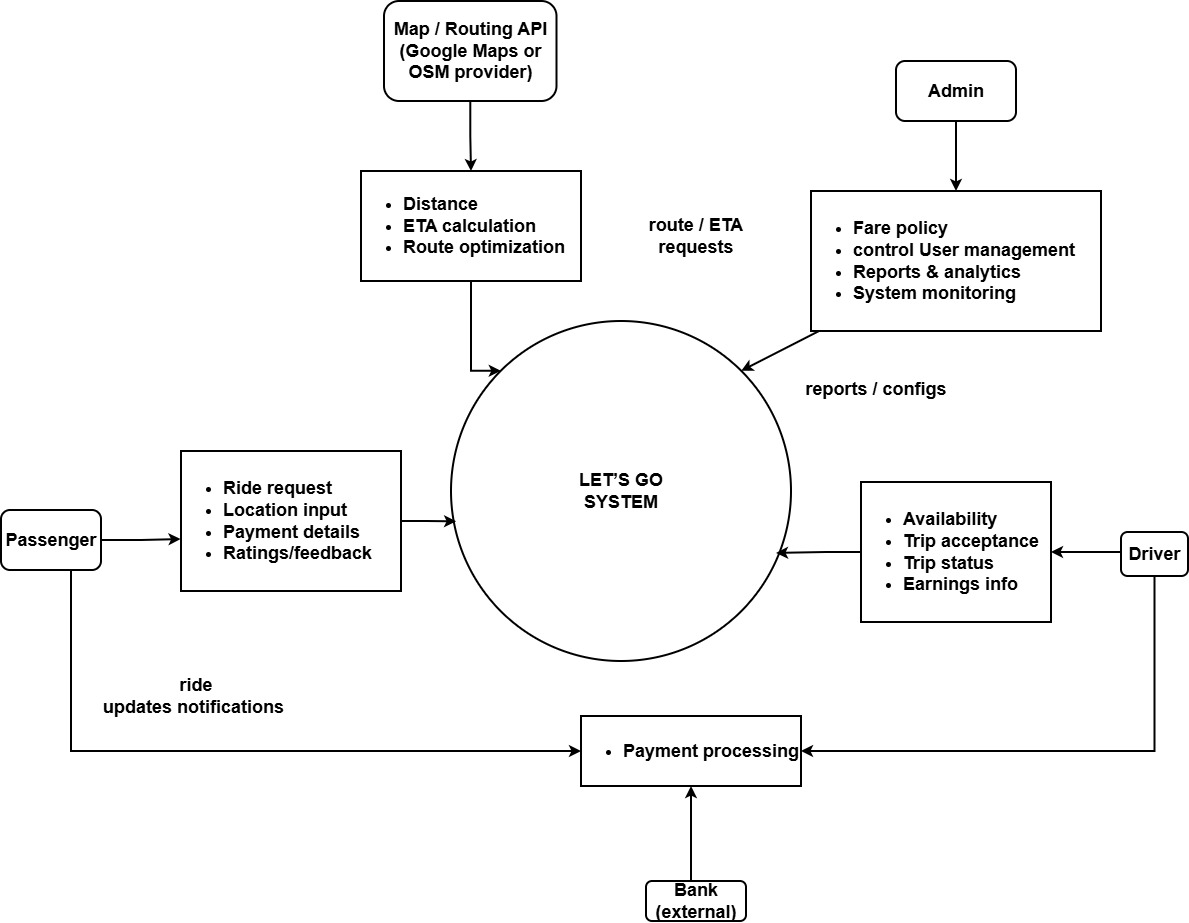
\includegraphics[width=0.9\textwidth,keepaspectratio,height=0.8\textheight]{assets/context Diagram-Page-2.jpg}
\caption{Context Diagram showing system boundary and interactions with external actors and services}
\label{fig:context}
\end{figure}

The context diagram illustrates the Lets Go Ride Sharing App system boundary and its interactions with external entities including Passengers, Drivers, Administrators, and third-party services (Map API, Notification Service, ML Service, Chatbot, Storage). Data flows represent ride requests, location updates, notifications, and document transfers.

%===========================================================
\section{Architectural Design}
%===========================================================

The Lets Go Ride Sharing App system is built under a hybrid architectural style consisting of two broad paradigms:
1. Multi-Tier Architecture for the overall system structure
2. Model-View-Controller (MVC) internally in the backend through Django framework

The combination offers separation of concerns, scalability, maintainability, and distributed deployment over several servers.

\subsection{Architecture Style (MVC + Multi-tier)}

\subsubsection{MVC Architecture (within Django backend servers)}

\begin{table}[htbp]
\centering
\caption{Backend MVC Structure}
\renewcommand{\arraystretch}{1.3}
\begin{tabularx}{\textwidth}{|X|X|X|}
\hline
\textbf{Layer} & \textbf{Component} & \textbf{Description} \\
\hline
Model & Django Models & Data representation and database ORM mappings \\
\hline
View & Templates / API serializers & Presentation logic for admin or API responses \\
\hline
Controller & Views & Request handling \& business logic \\
\hline
\end{tabularx}
\end{table}

Services are separated as independent modules:
\begin{itemize}
    \item AuthService
    \item RideManager
    \item VerificationManager
    \item NotificationService
    \item MLService
    \item ChatService
\end{itemize}
This ensures modularity, testability, and easier scalability.

\subsection{High-Level System Components}

The system is composed of:
\begin{itemize}
    \item \textbf{Client Layer:} Mobile apps (Passenger/Driver), Admin dashboard (web)
    \item \textbf{Application Layer:} Multiple identical backend servers running Django with JSON-based APIs for core features; mobile clients implement real-time behavior using periodic HTTP updates
    \item \textbf{External Services Layer:} Map API, Notifications (Supabase/FCM), Storage, ML recommendations, Chatbot
    \item \textbf{Data Layer:} PostgreSQL relational database, centralized and transaction-safe
\end{itemize}

\subsection{Multi-Tier Deployment Architecture}

\subsubsection{Tier 1 - Client Layer}
\begin{itemize}
    \item Flutter-based mobile applications for passengers and drivers
    \item HTML/CSS/JavaScript web-based admin dashboard
\end{itemize}

\subsubsection{Tier 2 - Application Layer}
\begin{itemize}
    \item Django backend servers with JSON-based APIs for authentication, rides, bookings, payments, safety, and administration
    \item Real-time behavior is achieved on the clients using periodic HTTP updates and push notifications where available
\end{itemize}

\subsubsection{Tier 3 - External Services Layer}
\begin{itemize}
    \item Map Service (OSRM/OpenStreetMap): Route calculation, distance, ETA
    \item Notification Service (FCM, SMS, Email)
    \item ML Recommendation Service: TF-IDF based ride recommendations
    \item Chatbot Service: Generative AI for FAQ support
    \item Storage Service: Document and image management
\end{itemize}

\subsubsection{Tier 4 - Data Layer}
\begin{itemize}
    \item PostgreSQL (Supabase) for transactional data
    \item Geospatial computations are handled in application logic for distance and route summaries
\end{itemize}

\subsection{External Services Integration}

Backend servers interface with external services through well-defined REST APIs with token-based authentication and fault-tolerant retry mechanisms.

\subsubsection{Map Service}
\begin{itemize}
    \item Reverse geocoding
    \item Route calculations
    \item Distance and ETA estimation
\end{itemize}

\subsubsection{Notification Service}
\begin{itemize}
    \item Push notifications via FCM
    \item Alerts for ride request, driver acceptance, SOS
\end{itemize}

\subsubsection{ML Recommendation Service}
\begin{itemize}
    \item Receives ride request data
    \item Returns list of recommended rides
    \item Uses TF-IDF similarity
\end{itemize}

\subsubsection{Chatbot Service}
\begin{itemize}
    \item Provides automated FAQ responses
\end{itemize}

\subsubsection{Storage Service}
\begin{itemize}
    \item Uploading profile images
    \item Uploading verification documents
    \item Generating signed URLs
\end{itemize}

\subsection{Architecture Diagram}

The architecture diagram illustrates the four tiers: Client Layer (Mobile Apps, Admin Web), Application Layer (Django Backend with MVC and JSON APIs), External Services Layer (Map, Notifications, ML, Chatbot, Storage), and Data Layer (PostgreSQL). Arrows indicate data flow and API interactions between components.

\begin{figure}[H]
\centering
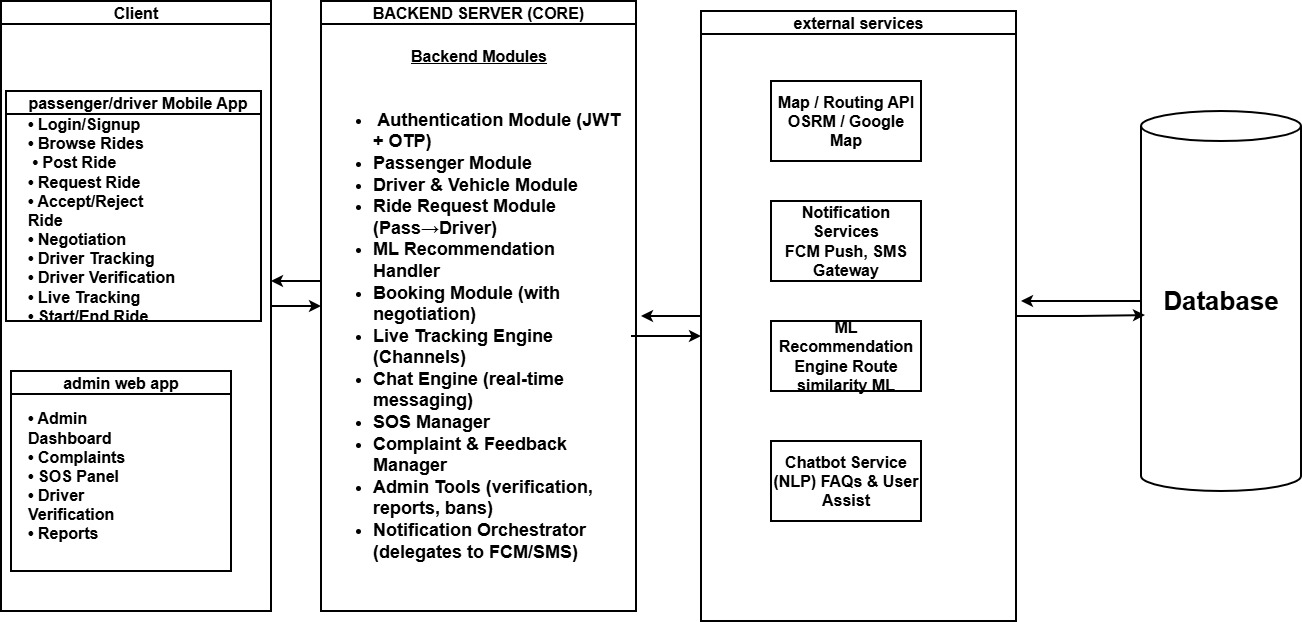
\includegraphics[width=0.9\textwidth,keepaspectratio,height=0.8\textheight]{assets/architecture.jpg}
\caption{High-level system architecture diagram showing multi-tier deployment and component interactions}
\label{fig:architecture}
\end{figure}

%===========================================================
\section{Design Models}
%===========================================================

This section presents detailed design models of the system. These models describe system behavior, structure, and interactions using UML diagrams. The models help developers understand system workflow before implementation.

%===========================================================
\subsection{Activity Diagrams}

Activity diagrams represent the workflow of different modules of the system. Each core module has a separate activity diagram showing user interaction, decision nodes, validation checks, and database/model interaction.

\subsubsection{Authentication \& Onboarding (Register, OTP, Admin verify)}

\begin{figure}[H]
\centering
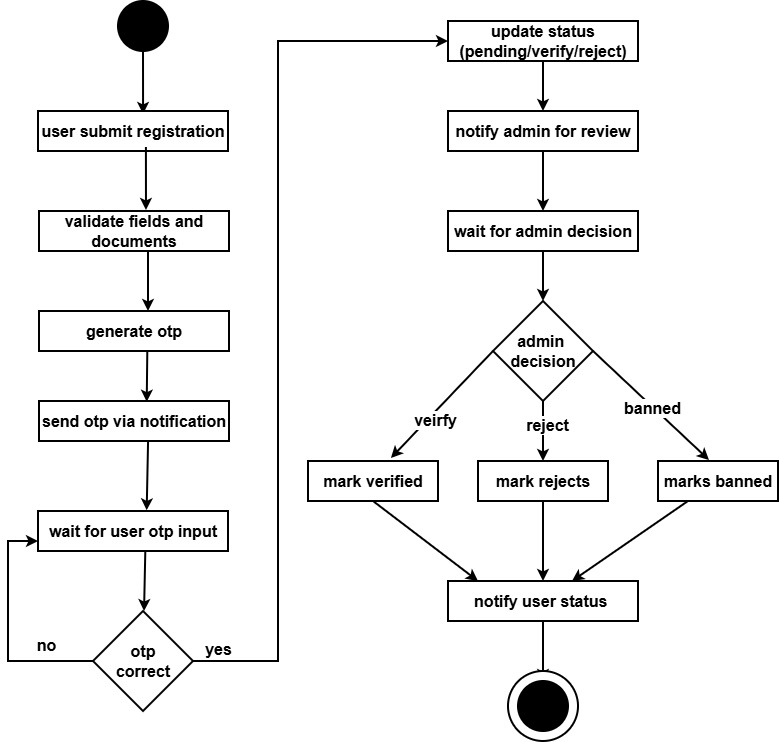
\includegraphics[width=0.8\textwidth,keepaspectratio,height=0.8\textheight]{assets/activity diagrams/activity_auth.jpg}
\caption{Activity Diagram - Authentication and Onboarding workflow}
\label{fig:activity_auth}
\end{figure}

This diagram illustrates the complete user registration and verification process: user enters details, uploads documents, receives OTP via email/SMS, verifies OTP, and awaits admin approval. Admin reviews documents and either verifies, rejects, or bans the user.

\clearpage

\subsubsection{Document Management (uploads \& verification)}

\begin{figure}[H]
\centering
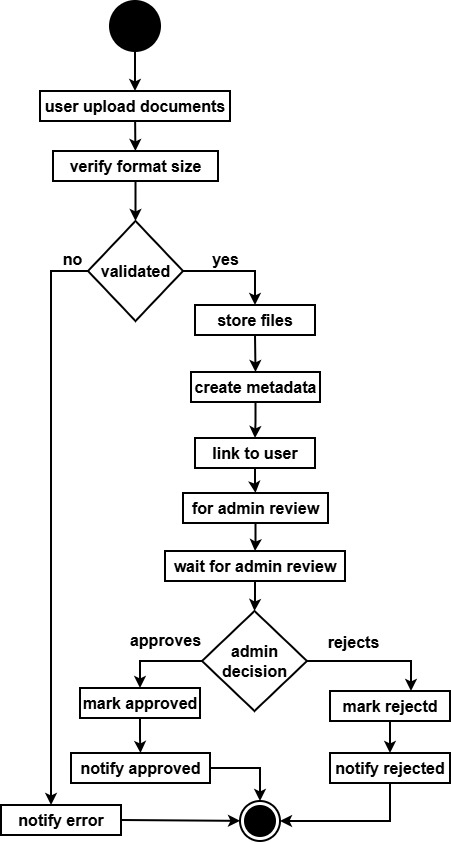
\includegraphics[width=0.6\textwidth,keepaspectratio,height=0.8\textheight]{assets/activity diagrams/activity_document.jpg}
\caption{Activity Diagram - Document Management workflow}
\label{fig:activity_document}
\end{figure}

Shows the process of document upload, validation (format/size), storage, and admin verification workflow including approval/rejection cycles.

\clearpage

\subsubsection{Vehicle Management (add/edit/delete vehicles)}

\begin{figure}[H]
\centering
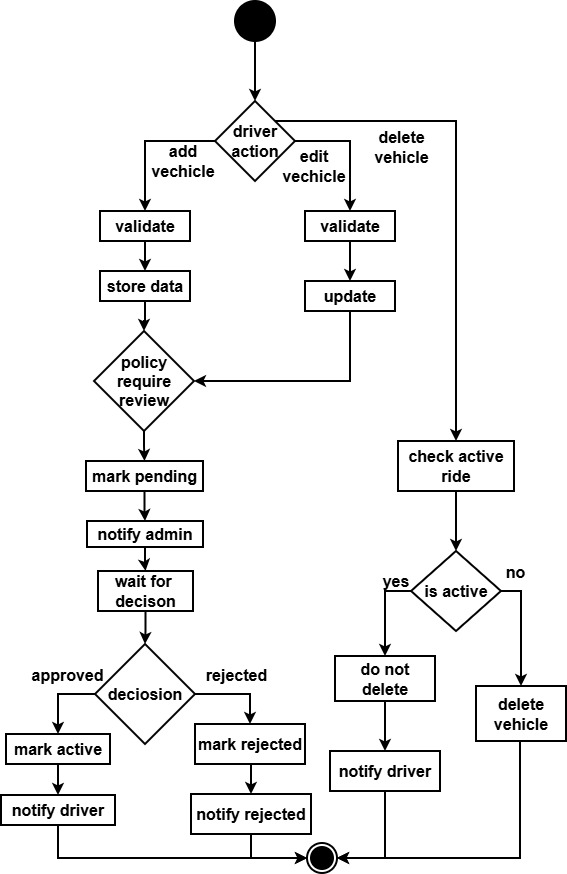
\includegraphics[width=0.8\textwidth,keepaspectratio,height=0.8\textheight]{assets/activity diagrams/module 3.jpg}
\caption{Activity Diagram - Vehicle Management workflow}
\label{fig:activity_vehicle}
\end{figure}

Depicts driver adding vehicle details, uploading images, system validation, and optional admin review for critical changes.

\clearpage

\subsubsection{Ride Management (create/edit/cancel, route \& stops)}

\begin{figure}[H]
\centering
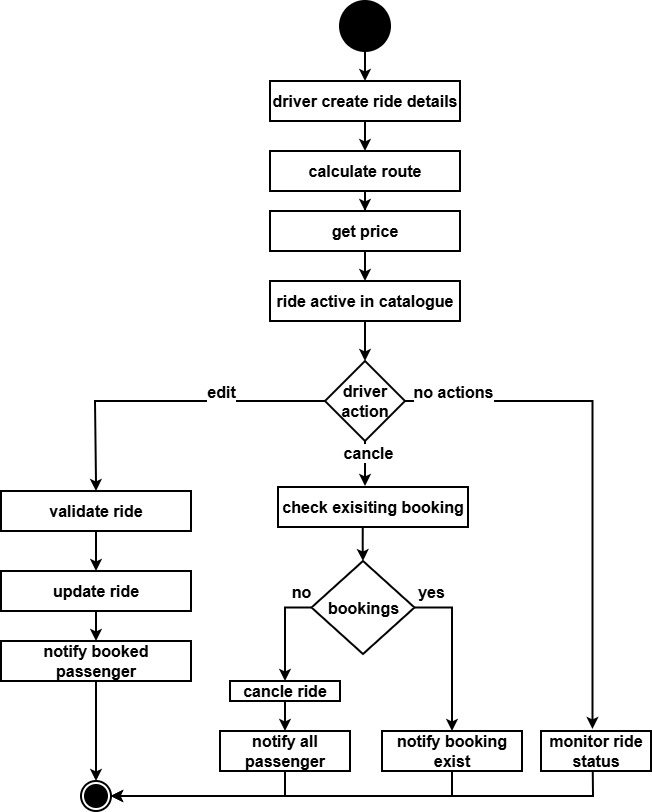
\includegraphics[width=0.8\textwidth,keepaspectratio,height=0.8\textheight]{assets/activity diagrams/module4.jpg}
\caption{Activity Diagram - Ride Management workflow}
\label{fig:activity_ride_mgmt}
\end{figure}

Illustrates driver creating a ride with map-based route editor, setting parameters (date/time, seats, gender preference, fare), validation, and publishing.

\clearpage

\subsubsection{Marketplace / Browse \& Search / Ride Details}

\begin{figure}[H]
\centering
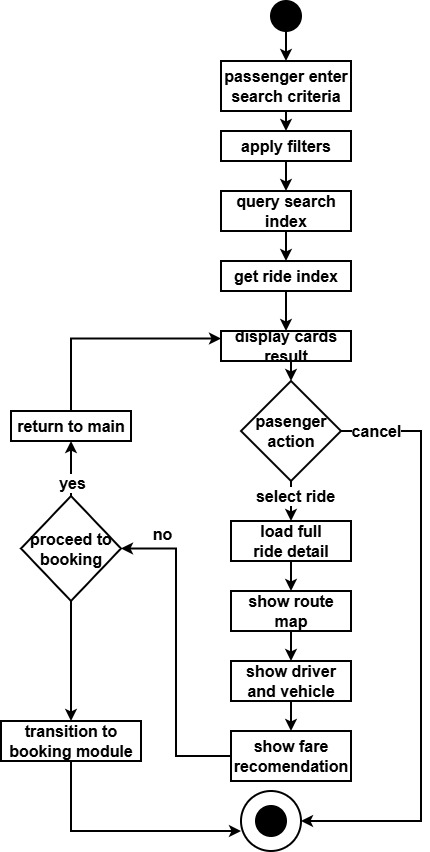
\includegraphics[width=0.8\textwidth,keepaspectratio,height=0.8\textheight]{assets/activity diagrams/module5.jpg}
\caption{Activity Diagram - Ride Browsing and Search workflow}
\label{fig:activity_browse}
\end{figure}

Shows passenger browsing available rides, applying filters, viewing ride cards with key information, and selecting a ride for detailed view.

\clearpage

\subsubsection{Booking \& Seat Management (select seats, lock seats)}

\begin{figure}[H]
\centering
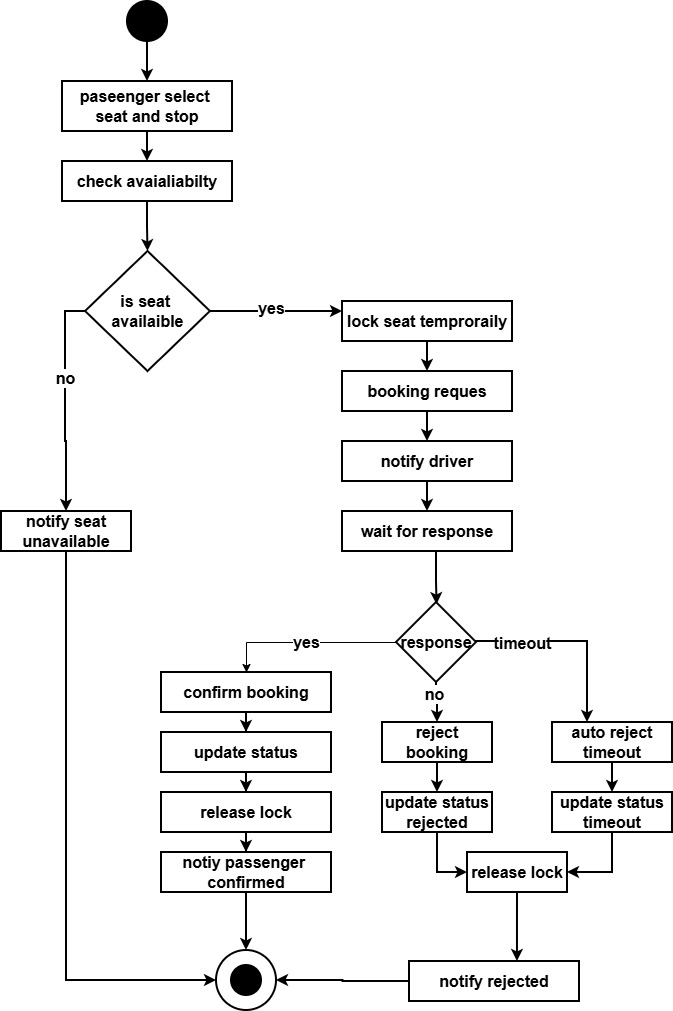
\includegraphics[width=0.8\textwidth,keepaspectratio,height=0.8\textheight]{assets/activity diagrams/module6.jpg}
\caption{Activity Diagram - Booking and Seat Management workflow}
\label{fig:activity_booking}
\end{figure}

Depicts passenger selecting pickup/drop stops, choosing seats (gender-based), special requests, fare calculation, seat locking, and driver acceptance/rejection.

\clearpage

\subsubsection{Post-Booking Chat / Messaging \& Broadcast}

\begin{figure}[H]
\centering
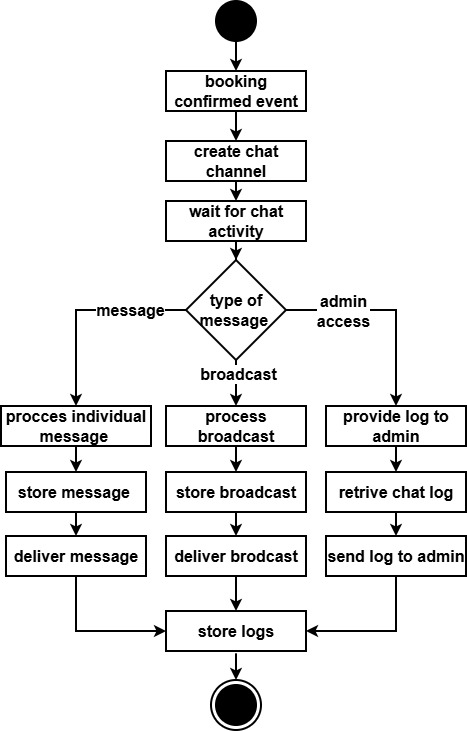
\includegraphics[width=0.8\textwidth,keepaspectratio,height=0.8\textheight]{assets/activity diagrams/module7.jpg}
\caption{Activity Diagram - Post-Booking Chat and Broadcast workflow}
\label{fig:activity_chat}
\end{figure}

Illustrates one-to-one messaging between driver and passengers, and driver broadcast to selected passengers.

\clearpage

\subsubsection{Scheduler / Pre-Ride Reminders \& Permission Prompt}

\begin{figure}[H]
\centering
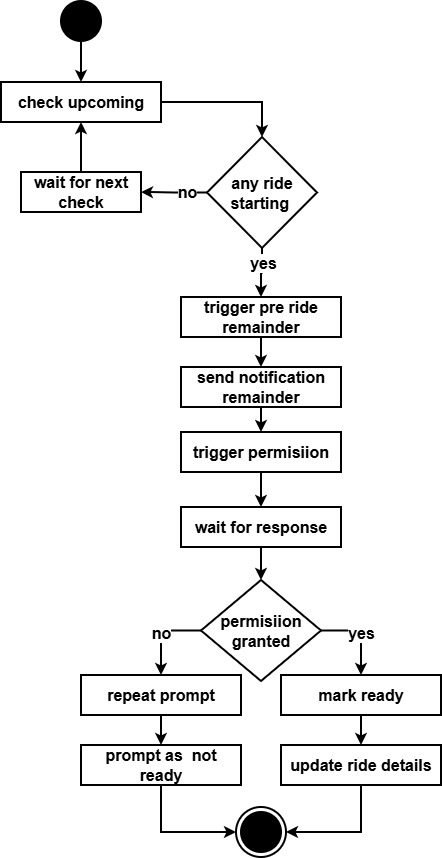
\includegraphics[width=0.8\textwidth,keepaspectratio,height=0.8\textheight]{assets/activity diagrams/module8.jpg}
\caption{Activity Diagram - Pre-Ride Reminders workflow}
\label{fig:activity_reminder}
\end{figure}

Shows scheduled reminders sent to driver and passengers, permission prompts, and readiness confirmation.

\clearpage

\subsubsection{Live Tracking \& Pickup Code (Start Ride / geofence)}

\begin{figure}[H]
\centering
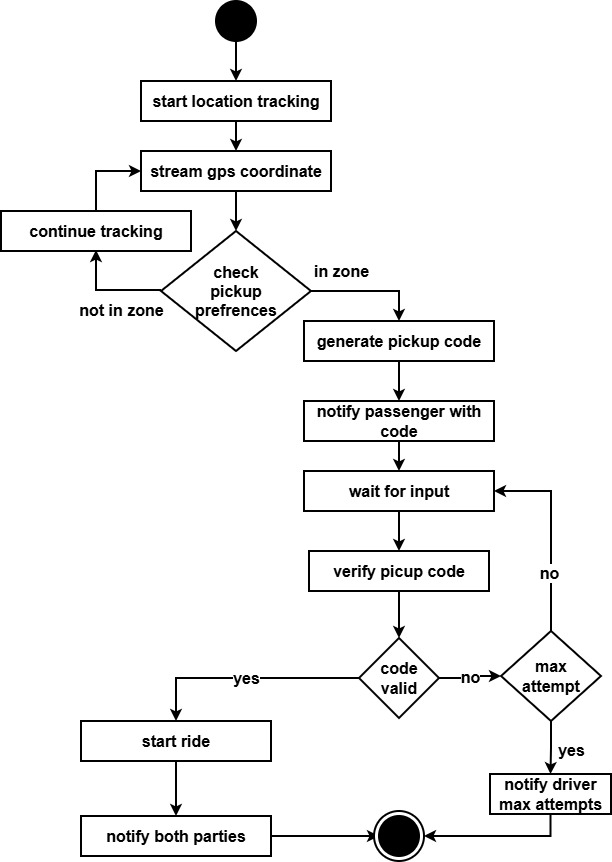
\includegraphics[width=0.8\textwidth,keepaspectratio,height=0.8\textheight]{assets/activity diagrams/module9.jpg}
\caption{Activity Diagram - Live Tracking and Pickup Code workflow}
\label{fig:activity_tracking}
\end{figure}

Depicts driver within geofence generating pickup code, passenger entering code, verification, and ride start.

\clearpage

\subsubsection{Payment \& Manual Payment Confirmation (cash / QR / bank transfer)}

\begin{figure}[H]
\centering
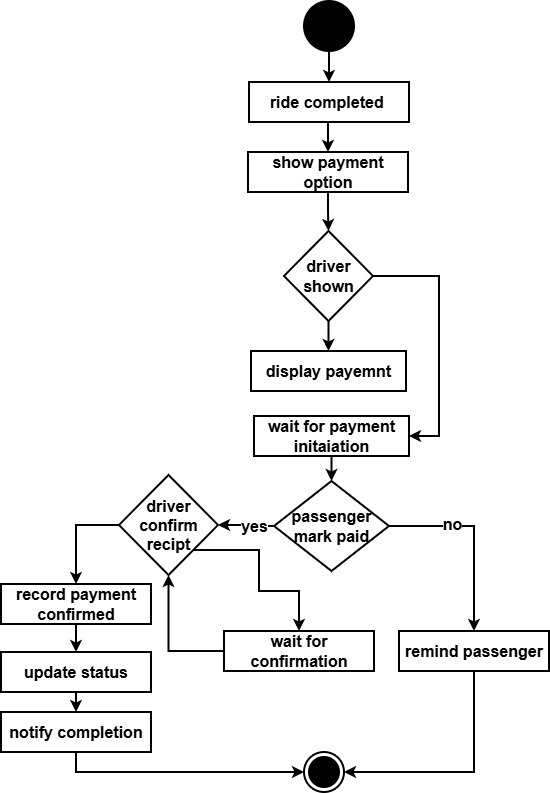
\includegraphics[width=0.8\textwidth,keepaspectratio,height=0.8\textheight]{assets/activity diagrams/module10.jpg}
\caption{Activity Diagram - Manual Payment Confirmation workflow}
\label{fig:activity_payment}
\end{figure}

Illustrates passenger marking reached, viewing driver bank details/QR, making payment, marking paid, and driver confirming receipt.

\clearpage

\subsubsection{Ratings \& Completion Workflow (mark reached, complete, rating)}

\begin{figure}[H]
\centering
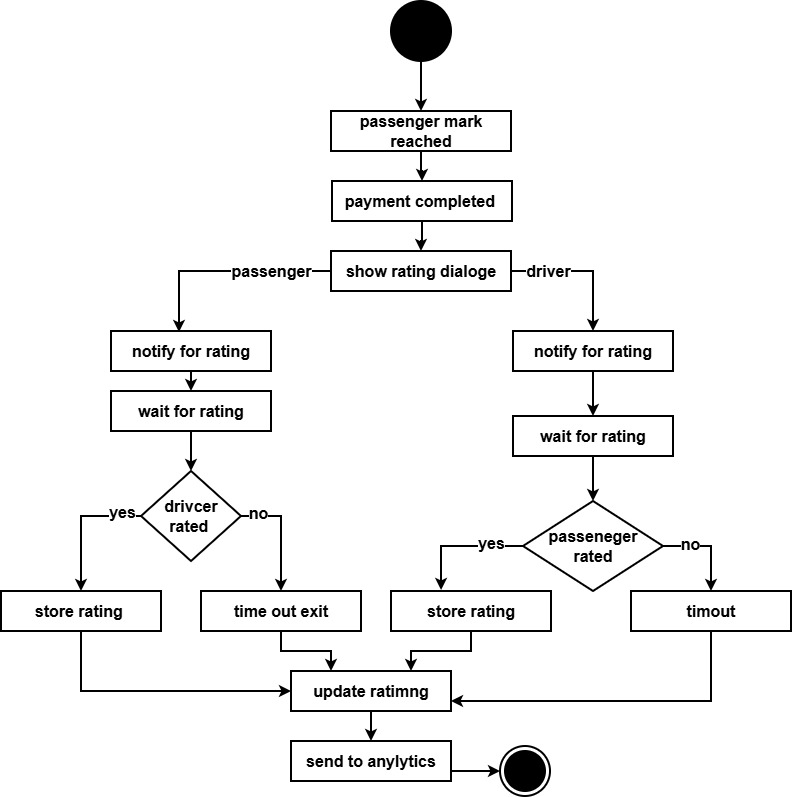
\includegraphics[width=0.8\textwidth,keepaspectratio,height=0.8\textheight]{assets/activity diagrams/module11.jpg}
\caption{Activity Diagram - Ratings and Completion workflow}
\label{fig:activity_rating}
\end{figure}

Shows passenger marking reached, rating prompt, driver marking complete, and mutual rating submission.

\clearpage

\subsubsection{SOS / Emergency \& Incident Management}

\begin{figure}[H]
\centering

\includegraphics[width=0.8\textwidth,keepaspectratio,height=0.8\textheight]{assets/activity diagrams/module 12.jpg}
\caption{Activity Diagram - SOS and Emergency workflow}
\label{fig:activity_sos}
\end{figure}

Depicts SOS trigger, immediate notifications to emergency contacts and admin, escalation timers, and incident resolution.

\clearpage

\subsubsection{Dispute Management \& Admin Dashboard (view \& resolve disputes)}

\begin{figure}[H]
\centering
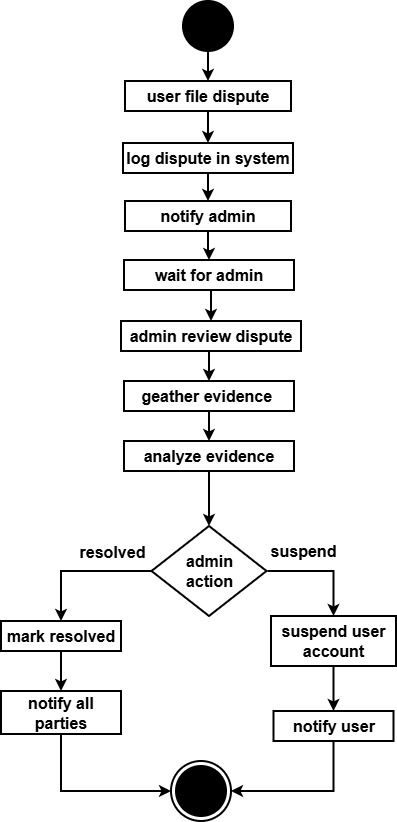
\includegraphics[width=0.8\textwidth,keepaspectratio,height=0.8\textheight]{assets/activity diagrams/module 13.jpg}
\caption{Activity Diagram - Dispute Management workflow}
\label{fig:activity_dispute}
\end{figure}

Illustrates user filing dispute, admin viewing evidence (chat logs, GPS traces), making resolution decision, and notifying parties.

\clearpage


%===========================================================
\subsection{Class Diagram}

The class diagram represents the static structure of the system by showing entities, their attributes, methods, and their relationships (association, aggregation, composition, inheritance). This diagram demonstrates encapsulation, inheritance, and associations as required by the object-oriented design methodology.

\begin{figure}[H]
\centering
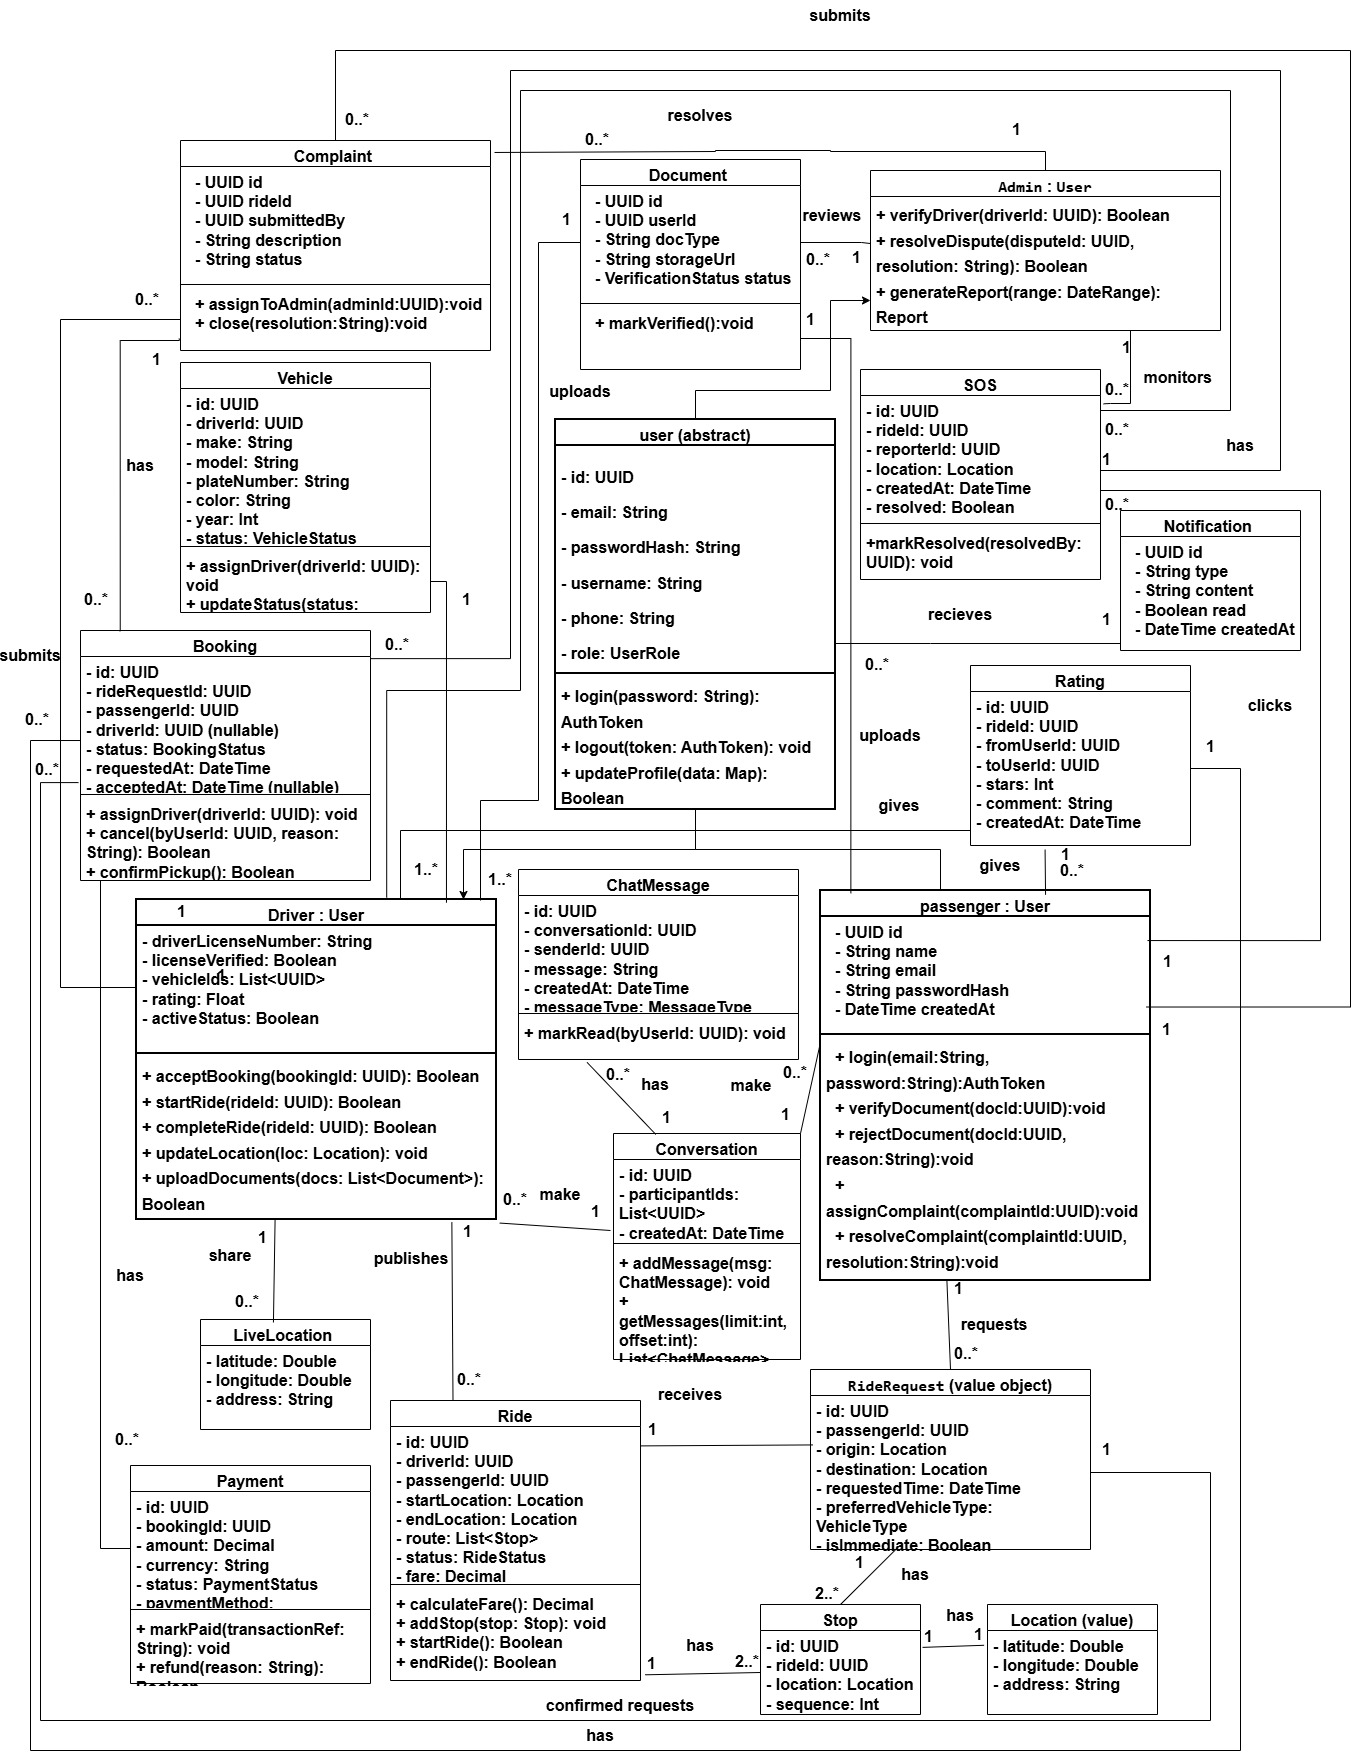
\includegraphics[width=0.9\textwidth,keepaspectratio,height=0.8\textheight]{assets/class diagram.jpg}
\caption{Comprehensive Class Diagram showing all system entities and relationships}
\label{fig:class}
\end{figure}

\subsubsection{Key Classes and Responsibilities}

\begin{itemize}
    \item \textbf{User (Abstract):} Base class with attributes: user\_id, name, email, password\_hash, role, created\_at. Methods: login(), logout(), updateProfile().
    
    \item \textbf{Passenger (inherits User):} Additional attributes: preference\_data (JSON). Methods: searchRides(), bookRide(), rateDriver(), fileComplaint().
    
    \item \textbf{Driver (inherits User):} Additional attributes: license\_number, verification\_status. Methods: createRide(), acceptBooking(), startRide(), completeRide().
    
    \item \textbf{Vehicle:} Attributes: vehicle\_id, driver\_id (FK), model, plate\_number, color, capacity, images. Methods: addVehicle(), updateVehicle(), deleteVehicle().
    
    \item \textbf{Ride:} Attributes: ride\_id, driver\_id (FK), route\_polyline, stops, departure\_time, available\_seats, gender\_preference, fare, status. Methods: createRide(), updateRide(), cancelRide().
    
    \item \textbf{Booking:} Attributes: booking\_id, ride\_id (FK), passenger\_id (FK), pickup\_stop, drop\_stop, seats\_booked, total\_fare, status, special\_requests. Methods: requestBooking(), acceptBooking(), rejectBooking(), cancelBooking().
    
    \item \textbf{Payment:} Attributes: payment\_id, booking\_id (FK), amount, method (cash/bank), status, timestamp. Methods: markPaid(), confirmReceived().
    
    \item \textbf{ChatMessage:} Attributes: message\_id, ride\_id (FK), sender\_id (FK), message\_text, timestamp, is\_broadcast. Methods: sendMessage(), getMessages().
    
    \item \textbf{Complaint:} Attributes: complaint\_id, ride\_id (FK), submitted\_by (FK), description, evidence\_links, status. Methods: fileComplaint(), resolveComplaint().
    
    \item \textbf{SOSRequest:} Attributes: sos\_id, user\_id (FK), ride\_id (FK), location, timestamp, status. Methods: triggerSOS(), escalateSOS(), resolveSOS().
    
    \item \textbf{User Document Fields:} User profile records store document/image URLs (CNIC, license, vehicle, profile photo) that reference uploaded files persisted in Supabase Storage. These fields support admin-driven verification workflows.
\end{itemize}

\subsubsection{Relationships}

\begin{itemize}
    \item \textbf{Inheritance:} Passenger and Driver inherit from User
    \item \textbf{One-to-Many:} Driver $\rightarrow$ Vehicle, Driver $\rightarrow$ Ride, Passenger $\rightarrow$ Booking, User $\rightarrow$ SOSRequest
    \item \textbf{Many-to-One:} Booking $\rightarrow$ Ride, Booking $\rightarrow$ Passenger, Ride $\rightarrow$ Driver
    \item \textbf{One-to-One:} Booking $\rightarrow$ Payment, Ride $\rightarrow$ Route (composition)
    \item \textbf{Many-to-Many:} Resolved through association classes like ChatMessage (connects Ride and User)
\end{itemize}

%===========================================================
\subsection{Sequence Diagrams}

Sequence diagrams show interaction between objects over time, illustrating request-response flows and component interactions.

\subsubsection{Sequence Diagram – Authentication (Login/Signup)}

\begin{figure}[H]
\centering
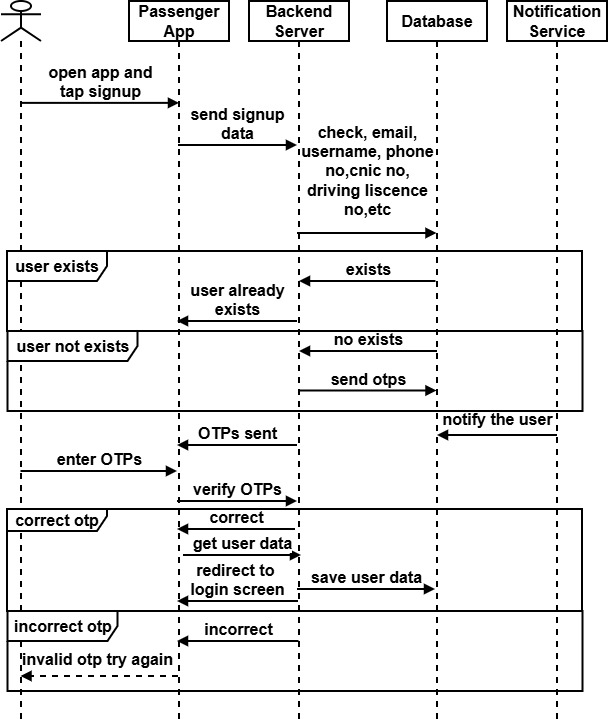
\includegraphics[width=0.8\textwidth,keepaspectratio,height=0.55\textheight]{assets/sequence diagrams/sequence diagram-USER SIGNUP (REGISTRATION).jpg}
\caption{Sequence Diagram - User Authentication (Signup and Login)}
\label{fig:seq_auth}
\end{figure}

\textbf{Description:} This diagram shows the interaction for user signup: User enters details, app sends to backend, backend validates, creates user record, sends OTP via Notification Service, user enters OTP, backend verifies and sets status to PENDING\_ADMIN\_VERIFICATION. For login: user enters credentials, backend validates, checks verification status, and returns JWT token.

\clearpage

\subsubsection{Sequence Diagram – Ride Posting}

\begin{figure}[H]
\centering
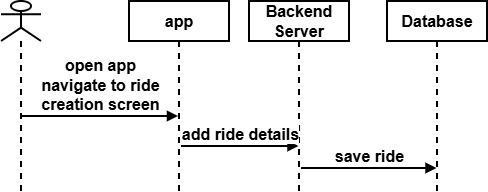
\includegraphics[width=1.0\textwidth,keepaspectratio,height=0.75\textheight]{assets/sequence diagrams/sequence diagram-post a ride.jpg}
\caption{Sequence Diagram - Driver Posting a Ride}
\label{fig:seq_ride_post}
\end{figure}

\textbf{Description:} Driver opens map, selects stops (interacting with Map Service for geocoding), enters ride parameters, backend validates, calculates fare (using FareCalculator), stores ride in database, and confirms creation. Ride becomes visible in marketplace.

\clearpage

\subsubsection{Sequence Diagram – Booking + Driver Acceptance}

\begin{figure}[H]
\centering
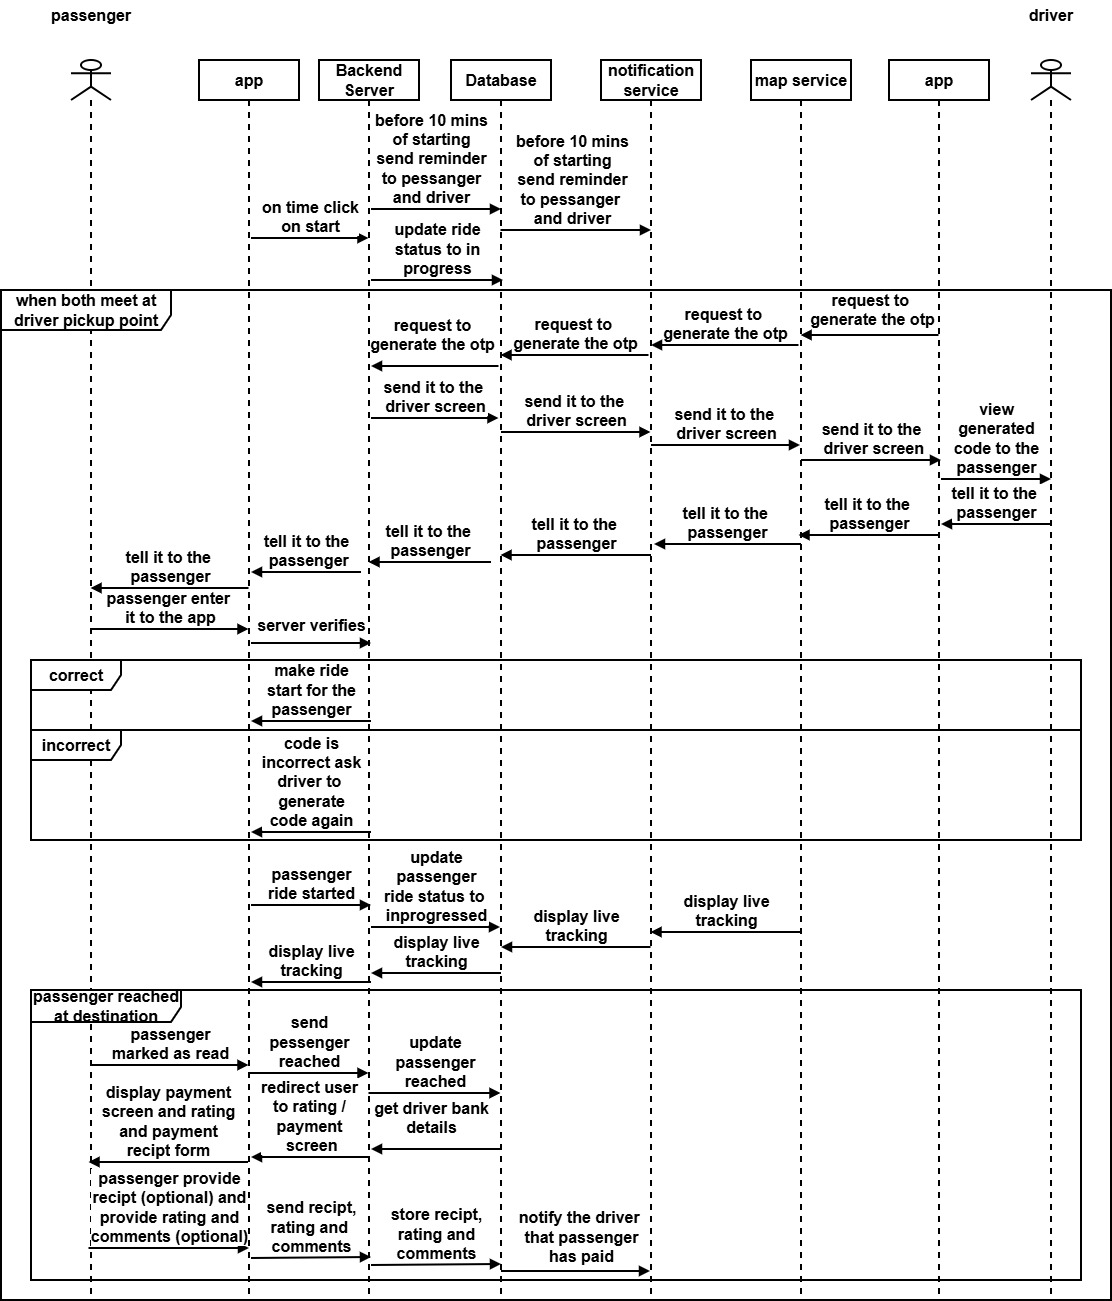
\includegraphics[width=0.9\textwidth,keepaspectratio,height=0.8\textheight]{assets/sequence diagrams/sequence diagram-post ride (starting to reached).jpg}
\caption{Sequence Diagram - Passenger Booking and Driver Acceptance}
\label{fig:seq_booking}
\end{figure}

\textbf{Description:} Passenger selects ride, selects stops/seats, backend calculates fare, locks seats, creates booking with REQUESTED status, sends notification to driver. Driver views request, accepts, backend updates booking to CONFIRMED, decrements available seats, sends confirmation to passenger.

\clearpage

\subsubsection{Sequence Diagram – Live Tracking + Ride Completion + Payment}

\begin{figure}[H]
\centering
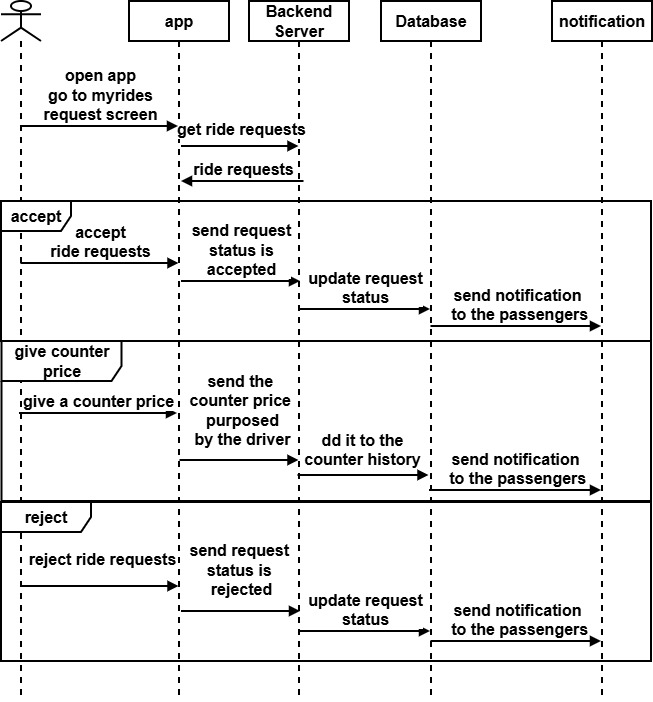
\includegraphics[width=0.9\textwidth,keepaspectratio,height=0.8\textheight]{assets/sequence diagrams/counter.jpg}
\caption{Sequence Diagram - Live Tracking, Ride Completion, and Payment}
\label{fig:seq_tracking}
\end{figure}

\textbf{Description:} Driver starts ride and sends periodic location updates to the backend via HTTP requests; passengers fetch updated tracking state through periodic HTTP updates. At destination, passenger marks reached, views driver bank details/QR, pays externally, marks paid. Driver confirms receipt, backend updates ride to COMPLETED, prompts ratings.

\clearpage

%===========================================================
\subsection{State Transition Diagrams}

State diagrams demonstrate how entities change state based on system events.

\subsubsection{State Transition Diagram – Ride Request and Booking}

\begin{figure}[H]
\centering
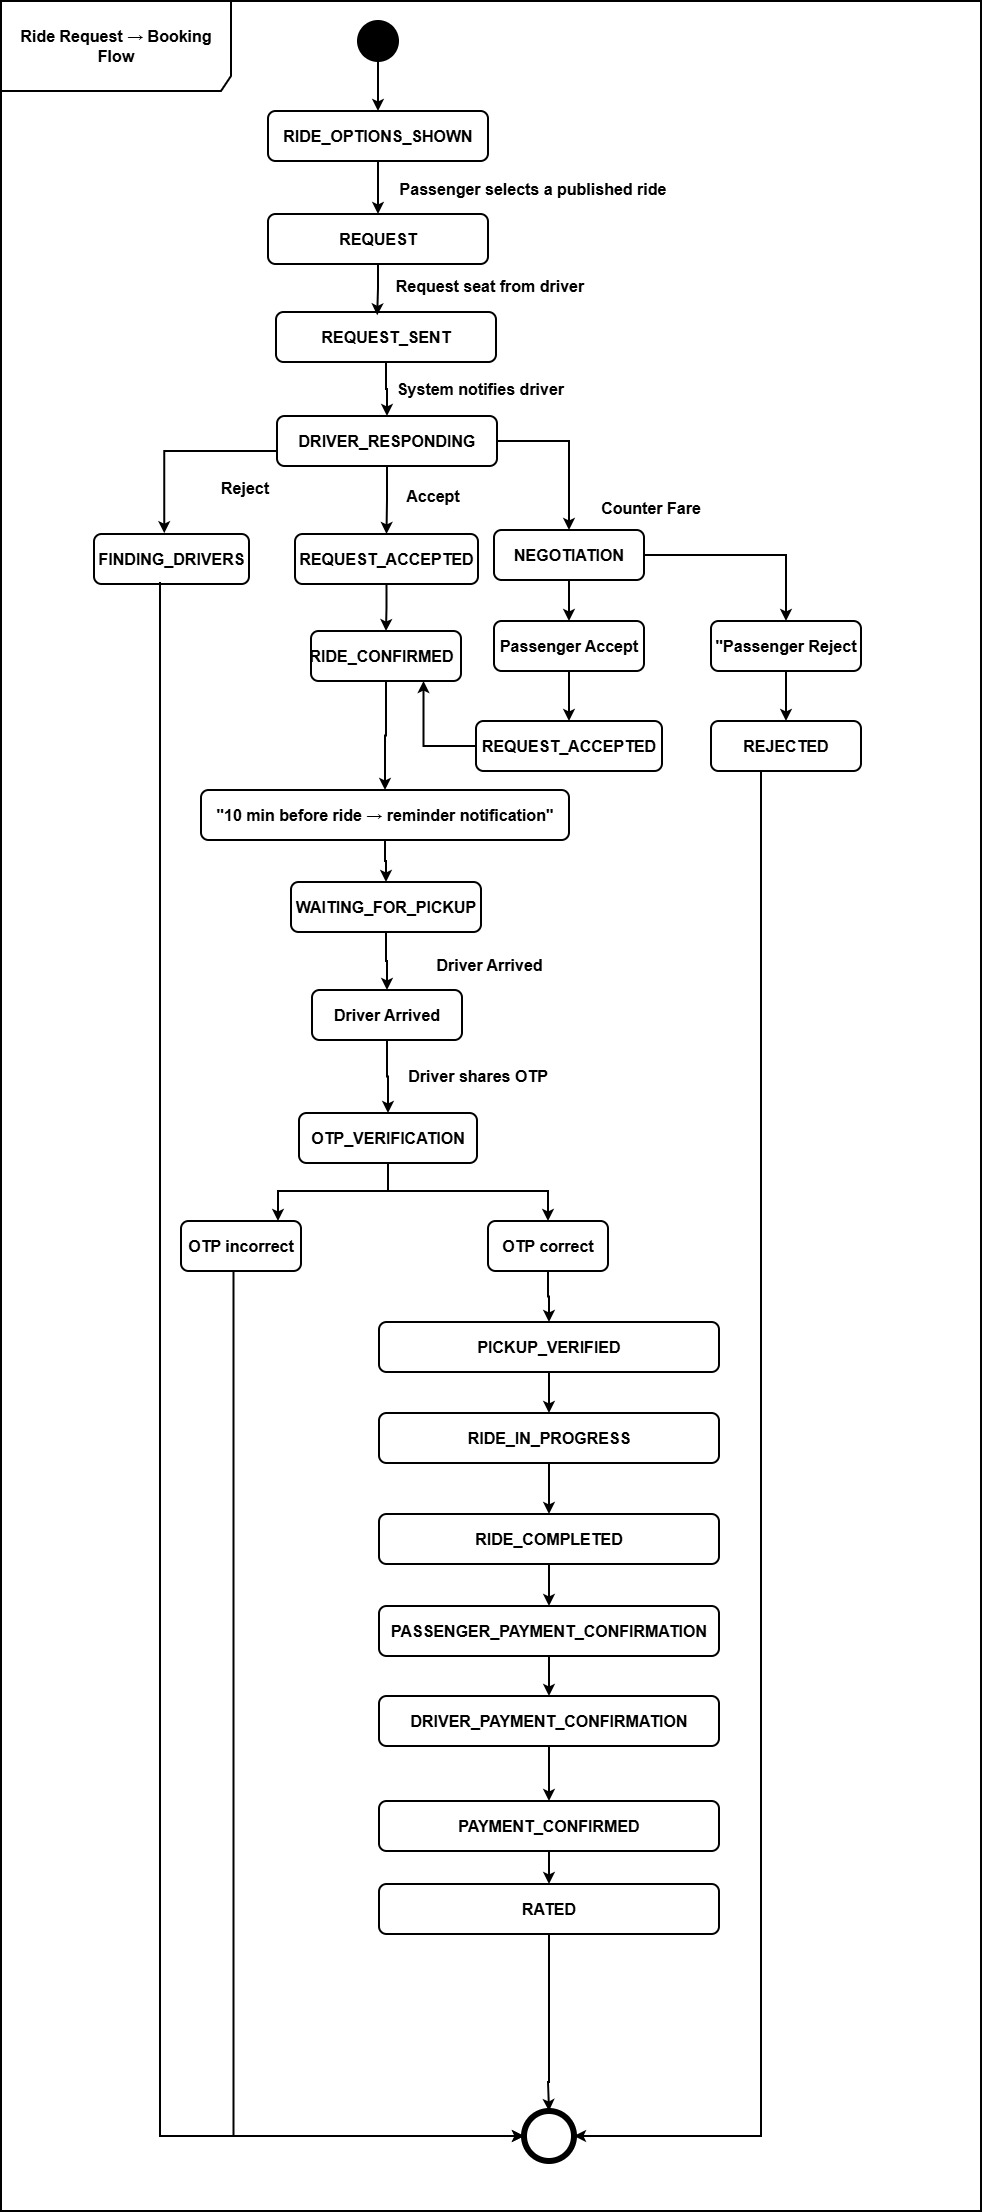
\includegraphics[width=0.9\textwidth,keepaspectratio,height=0.65\textheight]{assets/state transition diagrams/state transition-Ride Request → Booking Flow.jpg}
\caption{State Transition Diagram - Booking States}
\label{fig:state_booking}
\vspace{10pt}
\raggedright
\textbf{States:} 
\begin{itemize}[noitemsep,topsep=0pt]
    \item REQUESTED $\rightarrow$ (ACCEPTED $|$ REJECTED $|$ EXPIRED $|$ CANCELLED) $\rightarrow$ IN\_PROGRESS $\rightarrow$ COMPLETED
\end{itemize}
\textbf{Transitions:}
\begin{itemize}[noitemsep,topsep=0pt]
    \item Driver accepts (ACCEPTED), Driver rejects (REJECTED), Timeout (EXPIRED), Passenger cancels (CANCELLED), Ride starts (IN\_PROGRESS), Ride ends (COMPLETED)
\end{itemize}
\end{figure}

\subsubsection{State Transition Diagram – Driver States}

\begin{figure}[H]
\centering
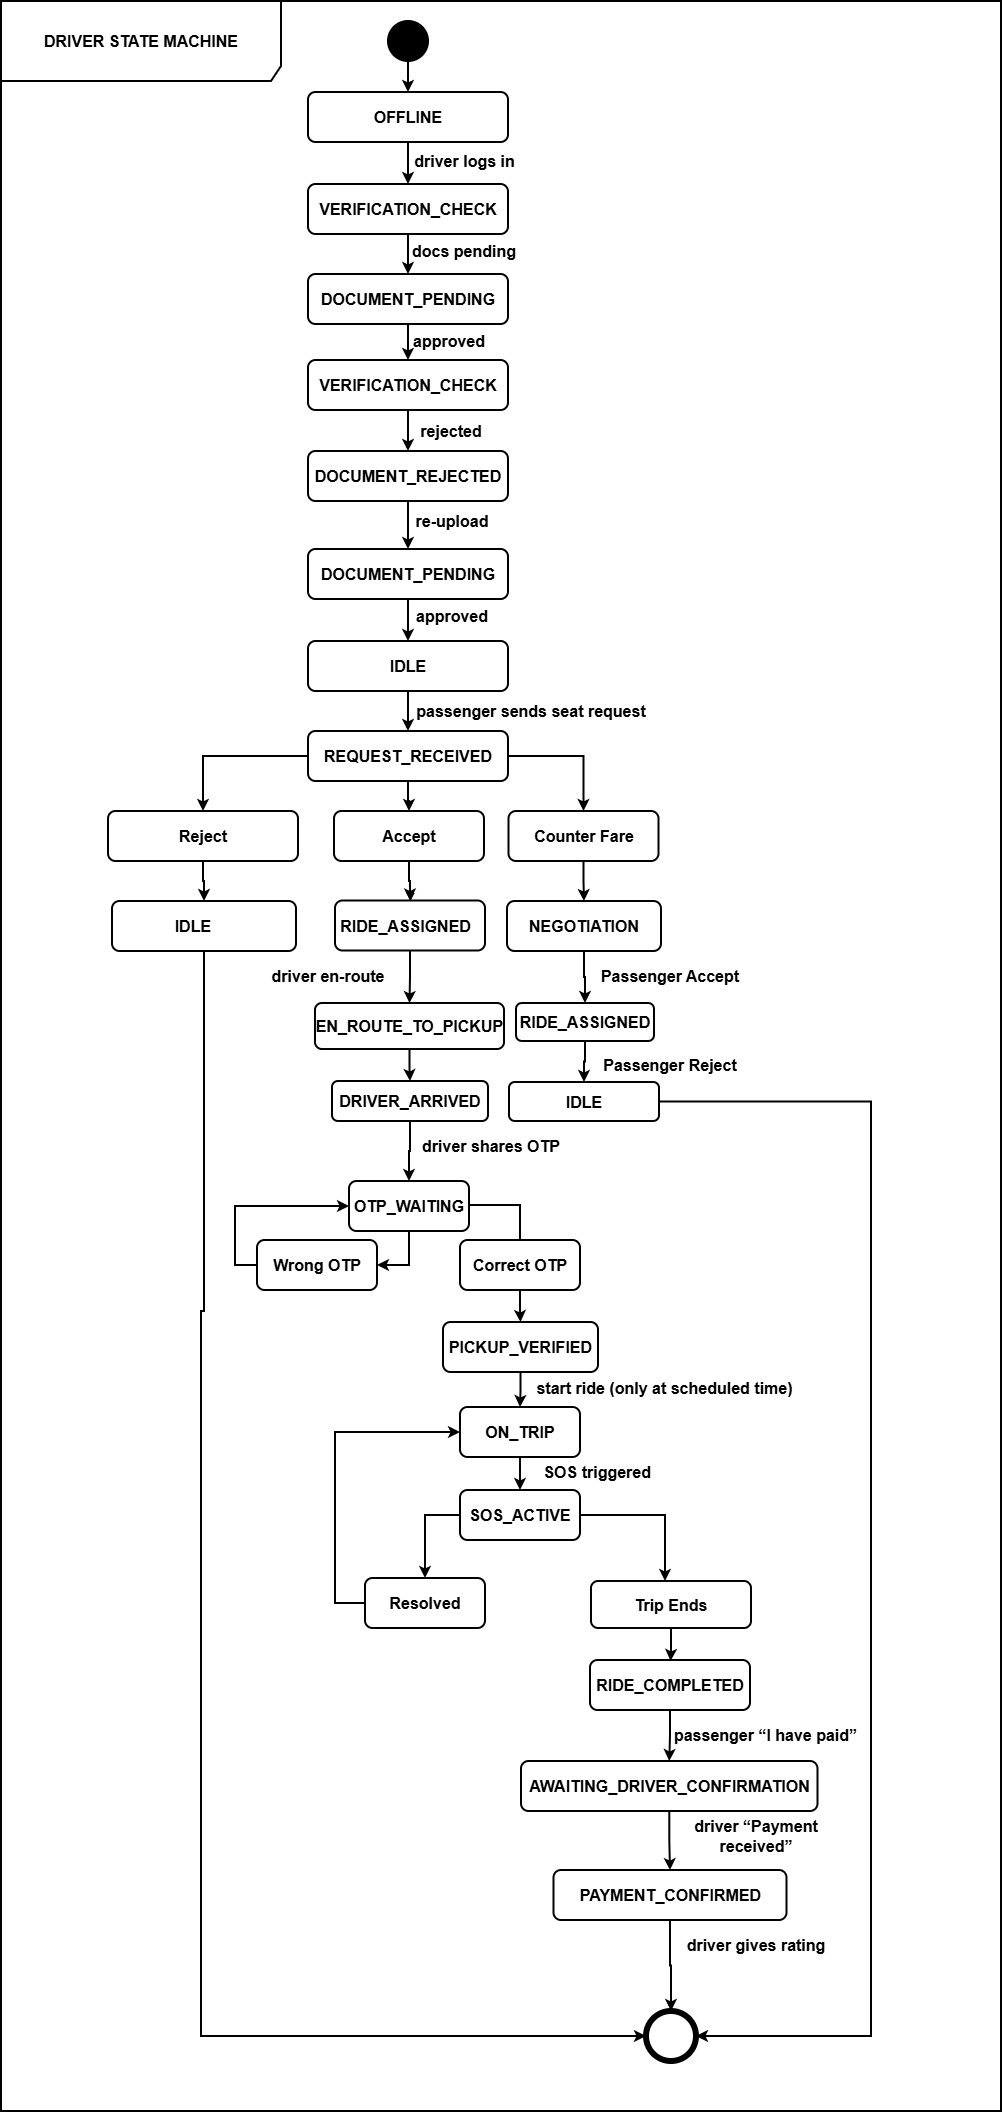
\includegraphics[width=0.9\textwidth,keepaspectratio,height=0.65\textheight]{assets/state transition diagrams/state transition-DRIVER STATE MACHINE.jpg}
\caption{State Transition Diagram - Driver States}
\label{fig:state_driver}
\vspace{10pt}
\raggedright
\textbf{States:} 
\begin{itemize}[noitemsep,topsep=0pt]
    \item OFFLINE $\rightarrow$ ONLINE $\rightarrow$ SEARCHING $\rightarrow$ ASSIGNED $\rightarrow$ EN\_ROUTE $\rightarrow$ ON\_RIDE $\rightarrow$ COMPLETED $\rightarrow$ ONLINE
\end{itemize}
\textbf{Transitions:}
\begin{itemize}[noitemsep,topsep=0pt]
    \item Driver logs in (ONLINE), receives request (SEARCHING), accepts (ASSIGNED), heading to pickup (EN\_ROUTE), passenger onboard (ON\_RIDE), ride ends (COMPLETED), becomes available (ONLINE)
\end{itemize}
\end{figure}

\subsubsection{State Transition Diagram – Passenger States}

\begin{figure}[H]
\centering
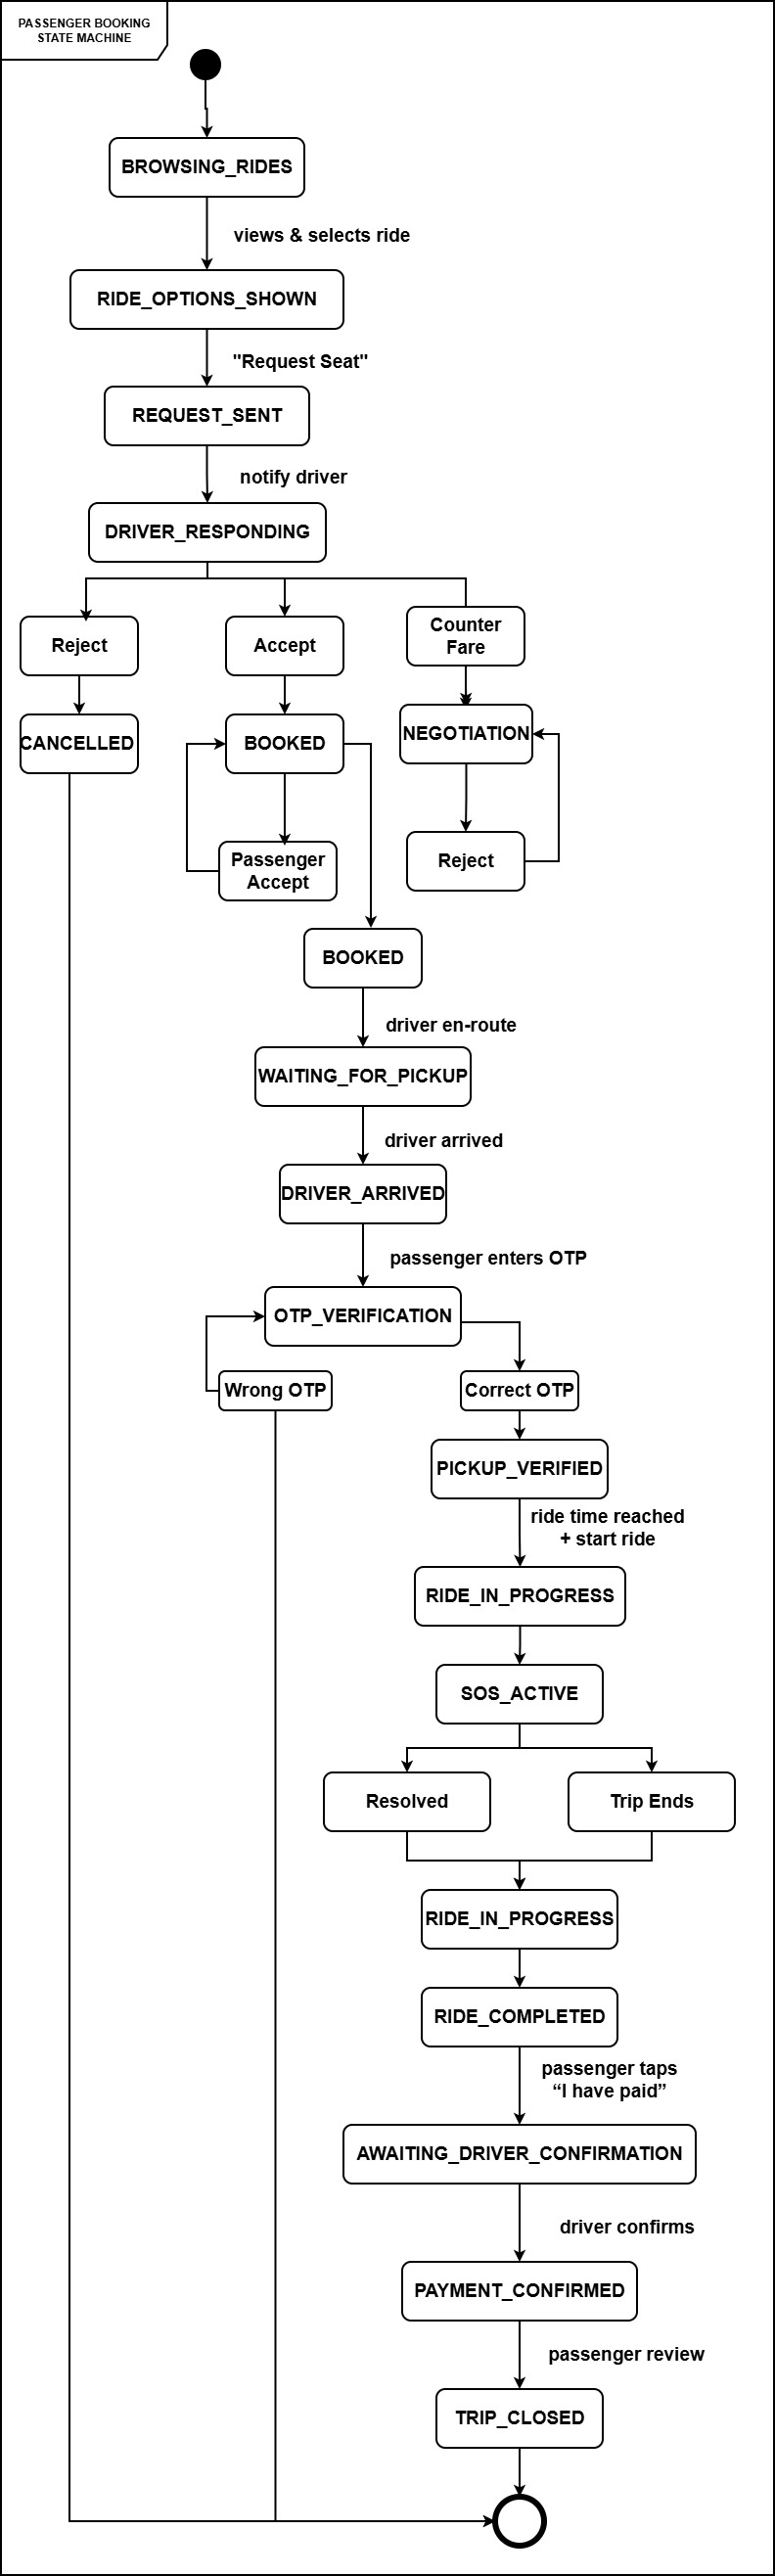
\includegraphics[width=0.9\textwidth,keepaspectratio,height=0.65\textheight]{assets/state transition diagrams/state transition-ASSENGER BOOKING STATE MACHINE.jpg}
\caption{State Transition Diagram - Passenger States}
\label{fig:state_passenger}
\vspace{10pt}
\raggedright
\textbf{States:} 
\begin{itemize}[noitemsep,topsep=0pt]
    \item IDLE $\rightarrow$ SEARCHING $\rightarrow$ BOOKED $\rightarrow$ WAITING $\rightarrow$ ON\_RIDE $\rightarrow$ COMPLETED $\rightarrow$ IDLE
\end{itemize}
\textbf{Transitions:}
\begin{itemize}[noitemsep,topsep=0pt]
    \item Searches rides (SEARCHING), books (BOOKED), driver accepted (WAITING), driver arrived/pickup (ON\_RIDE), dropped off (COMPLETED)
\end{itemize}
\end{figure}

\subsubsection{State Transition Diagram – SOS States}

\begin{figure}[H]
\centering
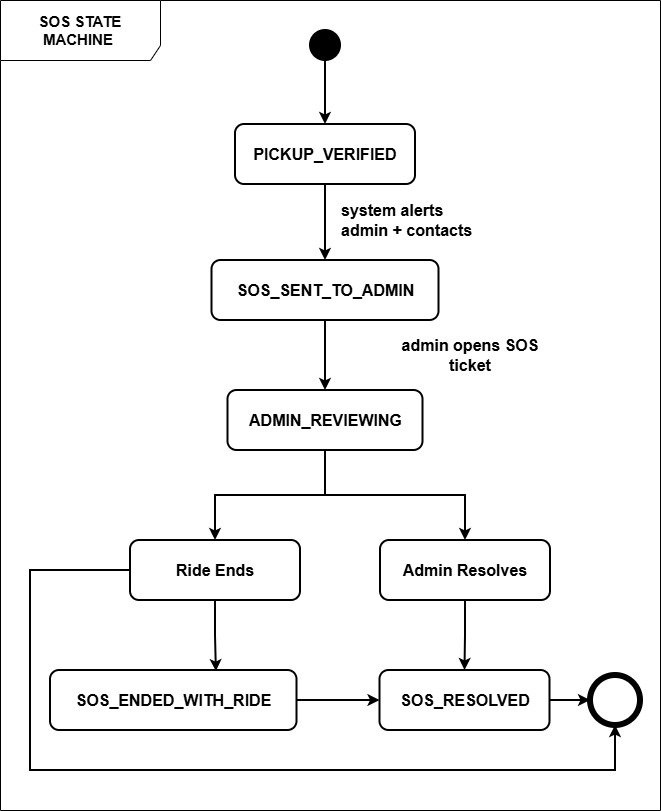
\includegraphics[width=0.9\textwidth,keepaspectratio,height=0.65\textheight]{assets/state transition diagrams/state transition-SOS STATE MACHINE — DRAW.IO READY.jpg}
\caption{State Transition Diagram - SOS States}
\label{fig:state_sos}
\vspace{10pt}
\raggedright
\textbf{States:} 
\begin{itemize}[noitemsep,topsep=0pt]
    \item INACTIVE $\rightarrow$ TRIGGERED $\rightarrow$ NOTIFIED $\rightarrow$ ACKNOWLEDGED $\rightarrow$ RESOLVED $\rightarrow$ INACTIVE
\end{itemize}
\textbf{Transitions:}
\begin{itemize}[noitemsep,topsep=0pt]
    \item User presses SOS (TRIGGERED), notifications sent (NOTIFIED), admin/contacts respond (ACKNOWLEDGED), situation resolved (RESOLVED)
\end{itemize}
\end{figure}

\subsubsection{Complaint and Dispute States Machine}

\begin{figure}[H]
\centering
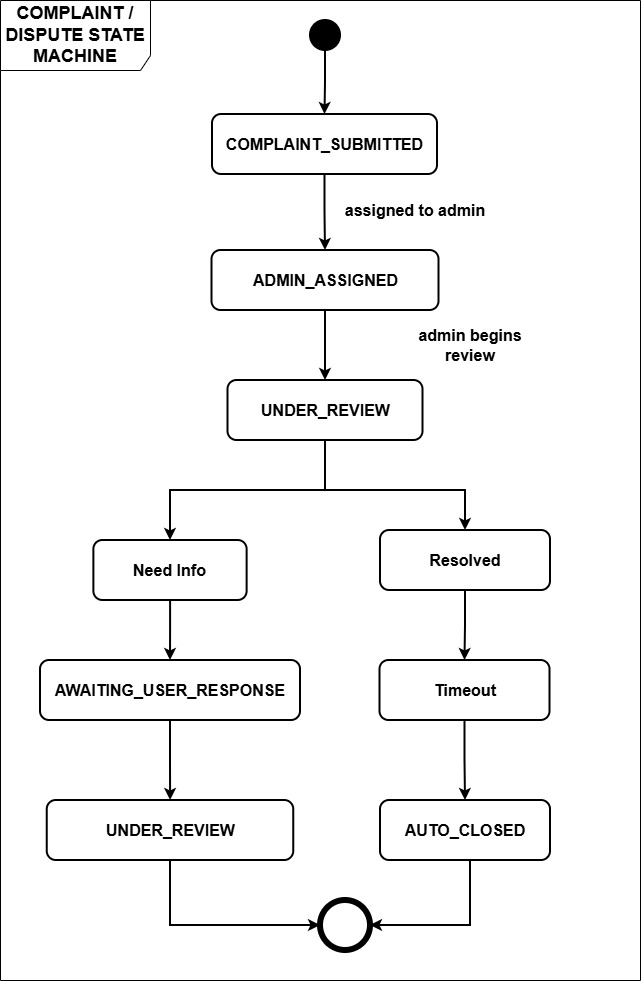
\includegraphics[width=0.9\textwidth,keepaspectratio,height=0.65\textheight]{assets/state transition diagrams/DISPUTE STATE MACHINE.jpg}
\caption{State Transition Diagram - Complaint and Dispute States}
\label{fig:state_dispute}
\vspace{10pt}
\raggedright
\textbf{States:} 
\begin{itemize}[noitemsep,topsep=0pt]
    \item FILED $\rightarrow$ UNDER\_REVIEW $\rightarrow$ (RESOLVED $|$ REJECTED $|$ ESCALATED)
\end{itemize}
\textbf{Transitions:}
\begin{itemize}[noitemsep,topsep=0pt]
    \item User files complaint (FILED), admin starts review (UNDER\_REVIEW), admin decides (RESOLVED/REJECTED), insufficient info (ESCALATED)
\end{itemize}
\end{figure}

\clearpage

\section{Data Flow Diagrams}
%===========================================================

Data Flow Diagrams (DFD) describe how data moves within the system at different levels of abstraction.

\subsection{Level 1 Data Flow Diagrams}

\subsubsection{Authentication \& Onboarding (Register, OTP, Admin verify)}

\begin{figure}[H]
\centering
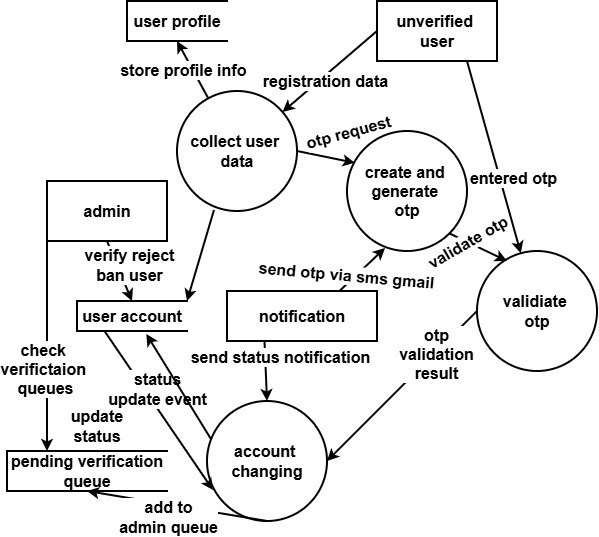
\includegraphics[width=0.9\textwidth,keepaspectratio,height=0.65\textheight]{assets/DFD/first registration module.jpg}
\caption{Level 1 DFD - Authentication and Onboarding}
\label{fig:dfd_auth}
\vspace{10pt}
\raggedright
\textbf{Processes:} 
\begin{itemize}[noitemsep,topsep=0pt]
    \item Register User, Send OTP, Verify OTP, Admin Verify Documents
\end{itemize}
\textbf{Data Stores:} 
\begin{itemize}[noitemsep,topsep=0pt]
    \item User DB, Document Store
\end{itemize}
\end{figure}

\subsubsection{Document Management (uploads \& verification)}

\begin{figure}[H]
\centering
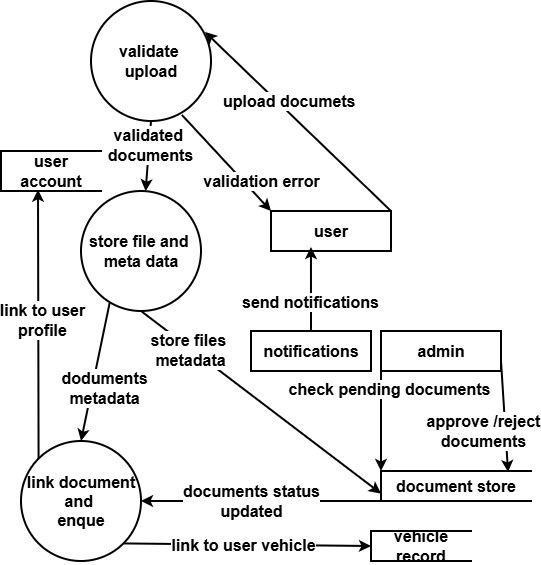
\includegraphics[width=0.9\textwidth,keepaspectratio,height=0.65\textheight]{assets/DFD/second module documents registartion.jpg}
\caption{Level 1 DFD - Document Management}
\label{fig:dfd_document}
\vspace{10pt}
\raggedright
\textbf{Processes:} 
\begin{itemize}[noitemsep,topsep=0pt]
    \item Upload Document, Validate Document, Store Document, Verify Document
\end{itemize}
\textbf{Data Stores:} 
\begin{itemize}[noitemsep,topsep=0pt]
    \item Document Store, User DB
\end{itemize}
\textbf{External Entities:} 
\begin{itemize}[noitemsep,topsep=0pt]
    \item User, Admin, Storage Service
\end{itemize}
\end{figure}


\subsubsection{Vehicle Management (add/edit/delete vehicles)}

\begin{figure}[H]
\centering
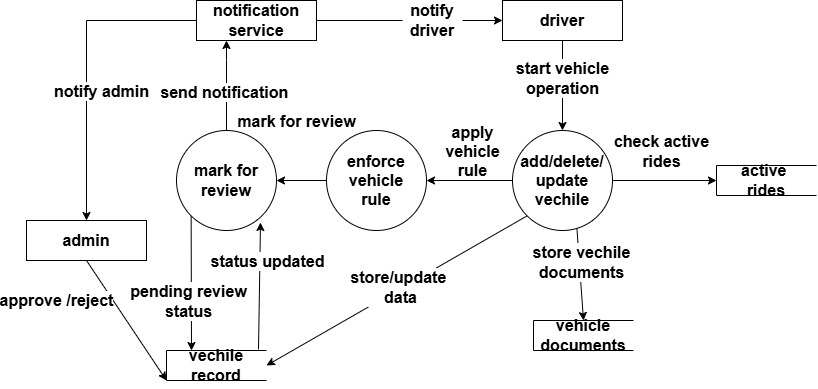
\includegraphics[width=0.9\textwidth,keepaspectratio,height=0.40\textheight]{assets/DFD/3rd module add vechile.jpg}
\caption{Level 1 DFD - Vehicle Management}
\label{fig:dfd_vehicle}
\vspace{10pt}
\raggedright
\textbf{Processes:} 
\begin{itemize}[noitemsep,topsep=0pt]
    \item Add Vehicle, Edit Vehicle, Delete Vehicle, Validate Vehicle
\end{itemize}
\textbf{Data Stores:} 
\begin{itemize}[noitemsep,topsep=0pt]
    \item Vehicle DB, User DB
\end{itemize}
\textbf{External Entities:} 
\begin{itemize}[noitemsep,topsep=0pt]
    \item Driver, Admin
\end{itemize}
\end{figure}


\subsubsection{Ride Management (create/edit/cancel, route \& stops)}

\begin{figure}[H]
\centering
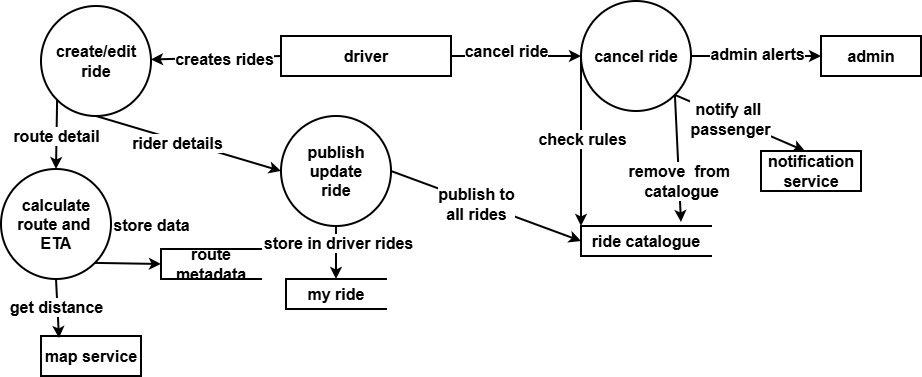
\includegraphics[width=0.9\textwidth,keepaspectratio,height=0.40\textheight]{assets/module_4_ride_management.jpg}
\caption{Level 1 DFD - Ride Management}
\label{fig:dfd_ride_mgmt}
\end{figure}

\clearpage

\raggedright
\textbf{Processes:} 
\begin{itemize}[noitemsep,topsep=0pt]
    \item Create Ride, Edit Ride, Cancel Ride, Calculate Fare
\end{itemize}
\textbf{Data Stores:} 
\begin{itemize}[noitemsep,topsep=0pt]
    \item Ride DB, Vehicle DB, Stop DB
\end{itemize}
\textbf{External Entities:} 
\begin{itemize}[noitemsep,topsep=0pt]
    \item Driver, Map Service
\end{itemize}

\subsubsection{Marketplace / Browse \& Search / Ride Details}

\begin{figure}[H]
\centering
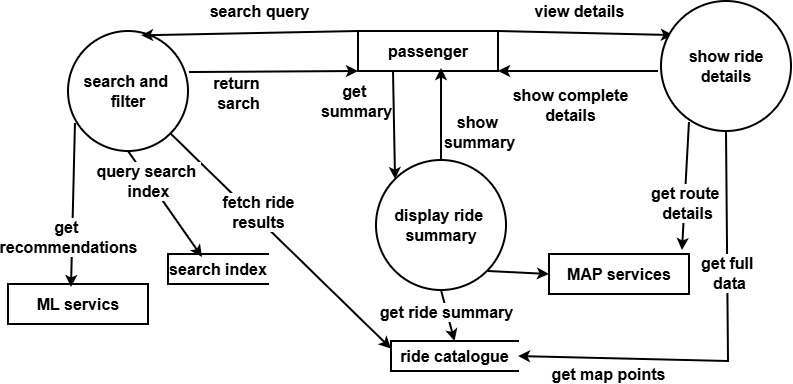
\includegraphics[width=0.9\textwidth,keepaspectratio,height=0.65\textheight]{assets/DFD/module 5 view rides.jpg}
\caption{Level 1 DFD - Ride Browsing and Search}
\label{fig:dfd_browse}
\vspace{10pt}
\raggedright
\textbf{Processes:} 
\begin{itemize}[noitemsep,topsep=0pt]
    \item Search Rides, Filter Rides, View Ride Details, Get Recommendations
\end{itemize}
\textbf{Data Stores:} 
\begin{itemize}[noitemsep,topsep=0pt]
    \item Ride DB, User DB
\end{itemize}
\textbf{External Entities:} 
\begin{itemize}[noitemsep,topsep=0pt]
    \item Passenger, ML Service
\end{itemize}
\end{figure}

\subsubsection{Booking \& Seat Management (select seats, lock seats)}

\begin{figure}[H]
\centering
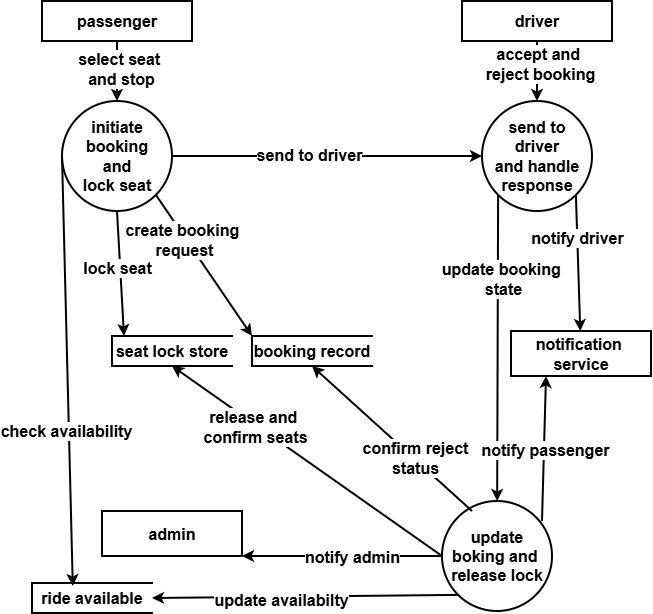
\includegraphics[width=0.9\textwidth,keepaspectratio,height=0.65\textheight]{assets/DFD/module 6 booking.jpg}
\caption{Level 1 DFD - Booking and Seat Management}
\label{fig:dfd_booking}
\vspace{10pt}
\raggedright
\textbf{Processes:} 
\begin{itemize}[noitemsep,topsep=0pt]
    \item Select Stops, Select Seats, Calculate Fare, Lock Seats, Create Booking
\end{itemize}
\textbf{Data Stores:} 
\begin{itemize}[noitemsep,topsep=0pt]
    \item Booking DB, Ride DB
\end{itemize}
\textbf{External Entities:} 
\begin{itemize}[noitemsep,topsep=0pt]
    \item Passenger, Driver
\end{itemize}
\end{figure}

\subsubsection{Post-Booking Chat / Messaging \& Broadcast}

\begin{figure}[H]
\centering
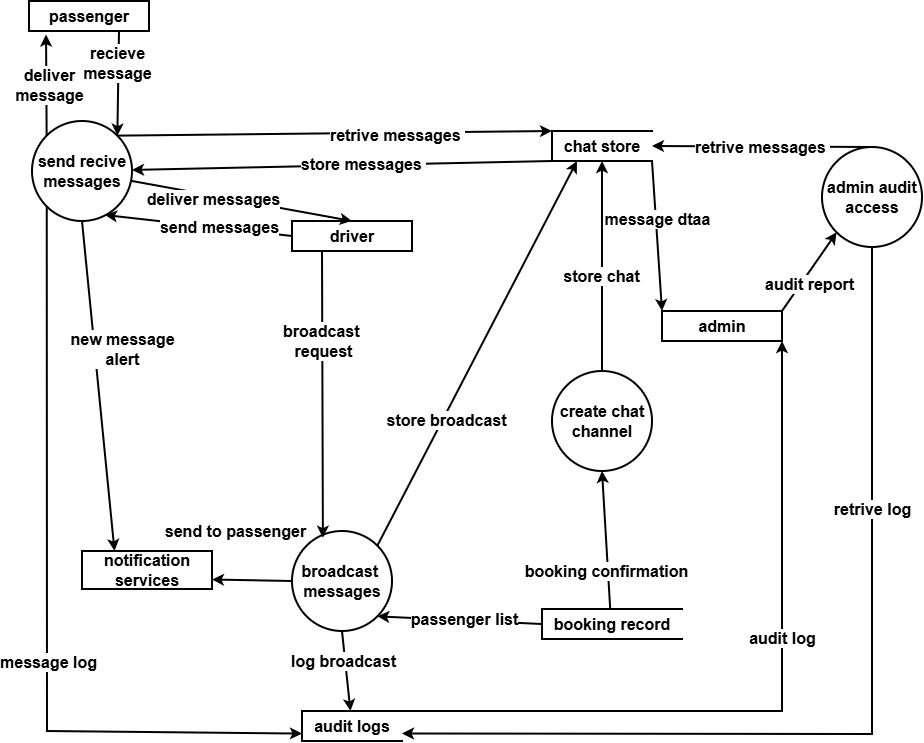
\includegraphics[width=0.9\textwidth,keepaspectratio,height=0.65\textheight]{assets/DFD/module 7 chat and message.jpg}
\caption{Level 1 DFD - Post-Booking Chat}
\label{fig:dfd_chat}
\vspace{10pt}
\raggedright
\textbf{Processes:} 
\begin{itemize}[noitemsep,topsep=0pt]
    \item Send Message, Broadcast Message, Store Message, Deliver Notification
\end{itemize}
\textbf{Data Stores:} 
\begin{itemize}[noitemsep,topsep=0pt]
    \item Chat DB
\end{itemize}
\textbf{External Entities:} 
\begin{itemize}[noitemsep,topsep=0pt]
    \item Passenger, Driver, Notification Service
\end{itemize}
\end{figure}


\subsubsection{Scheduler / Pre-Ride Reminders \& Permission Prompt}

\begin{figure}[H]
\centering
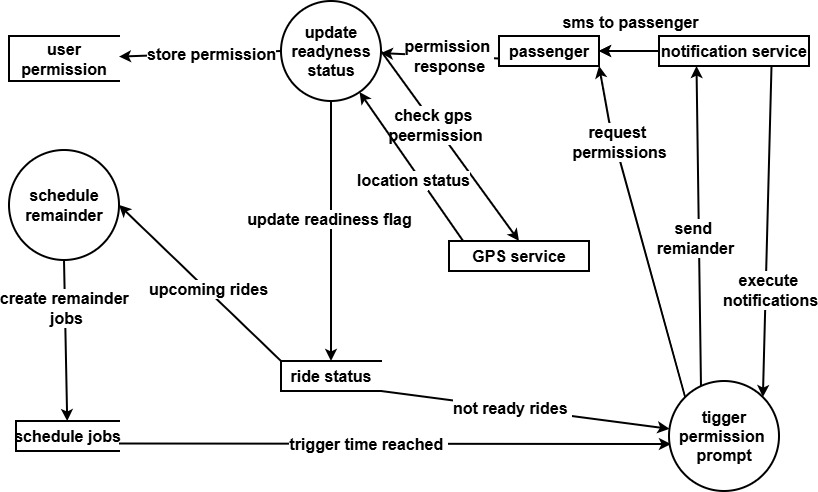
\includegraphics[width=0.9\textwidth,keepaspectratio,height=0.65\textheight]{assets/DFD/module 8 notification handlers.jpg}
\caption{Level 1 DFD - Pre-Ride Reminders}
\label{fig:dfd_reminder}
\vspace{10pt}
\raggedright
\textbf{Processes:} 
\begin{itemize}[noitemsep,topsep=0pt]
    \item Schedule Reminders, Send Reminders, Check Permissions, Update Readiness
\end{itemize}
\textbf{Data Stores:} 
\begin{itemize}[noitemsep,topsep=0pt]
    \item Ride DB, User DB
\end{itemize}
\textbf{External Entities:} 
\begin{itemize}[noitemsep,topsep=0pt]
    \item Passenger, Driver, Notification Service
\end{itemize}
\end{figure}

\subsubsection{Live Tracking \& Pickup Code (Start Ride / geofence)}

\begin{figure}[H]
\centering
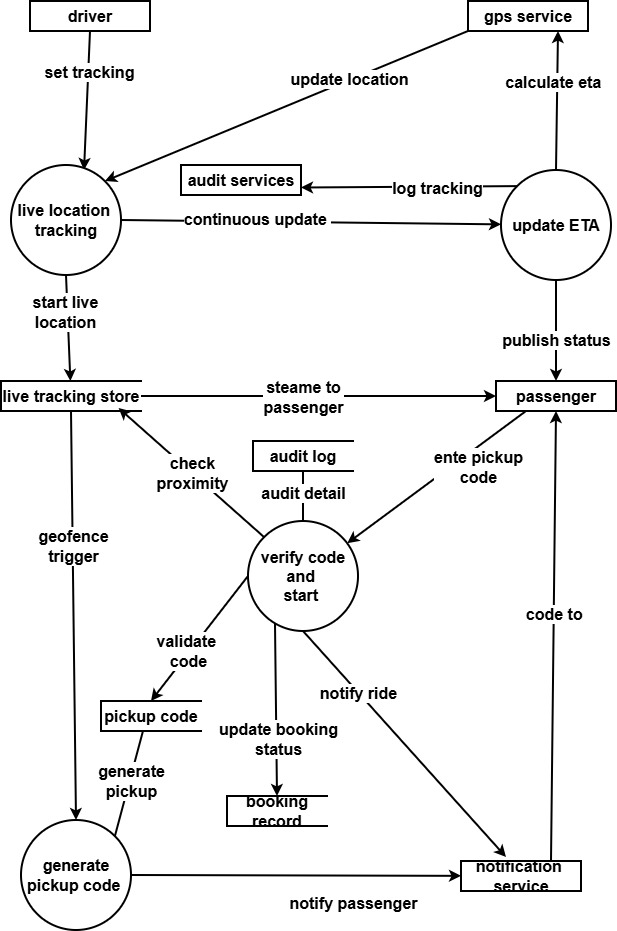
\includegraphics[width=0.9\textwidth,keepaspectratio,height=0.65\textheight]{assets/DFD/module 9 code verify.jpg}
\caption{Level 1 DFD - Live Tracking and Pickup Code}
\label{fig:dfd_tracking}
\vspace{10pt}
\raggedright
\textbf{Processes:} 
\begin{itemize}[noitemsep,topsep=0pt]
    \item Update Location, Broadcast Location, Generate Code, Verify Code, Start Ride
\end{itemize}
\textbf{Data Stores:} 
\begin{itemize}[noitemsep,topsep=0pt]
    \item Location DB, Ride DB
\end{itemize}
\textbf{External Entities:} 
\begin{itemize}[noitemsep,topsep=0pt]
    \item Driver, Passenger, Map Service
\end{itemize}
\end{figure}


\subsubsection{Payment \& Manual Payment Confirmation}

\begin{figure}[H]
\centering
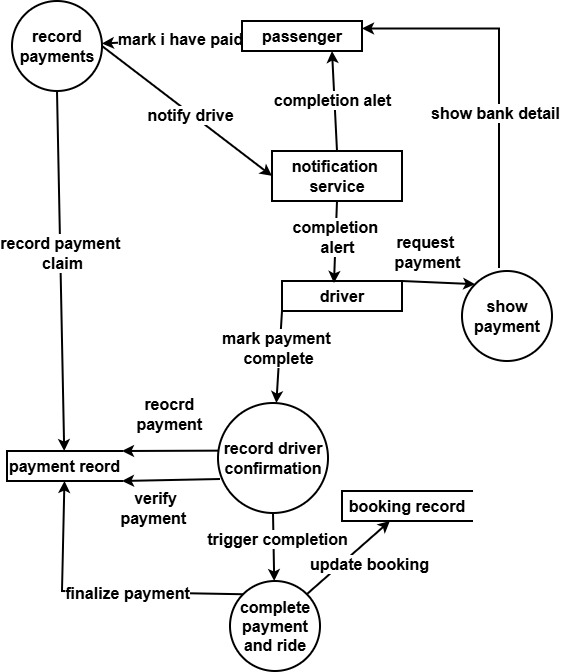
\includegraphics[width=0.9\textwidth,keepaspectratio,height=0.65\textheight]{assets/DFD/module 10 payment.jpg}
\caption{Level 1 DFD - Payment and Manual Confirmation}
\label{fig:dfd_payment}
\vspace{10pt}
\raggedright
\textbf{Processes:} 
\begin{itemize}[noitemsep,topsep=0pt]
    \item Show Payment Details, Mark Paid, Confirm Receipt, Update Ride Status
\end{itemize}
\textbf{Data Stores:} 
\begin{itemize}[noitemsep,topsep=0pt]
    \item Payment DB, Ride DB
\end{itemize}
\textbf{External Entities:} 
\begin{itemize}[noitemsep,topsep=0pt]
    \item Passenger, Driver, Notification Service
\end{itemize}
\end{figure}


\subsubsection{Ratings \& Completion Workflow}

\begin{figure}[H]
\centering
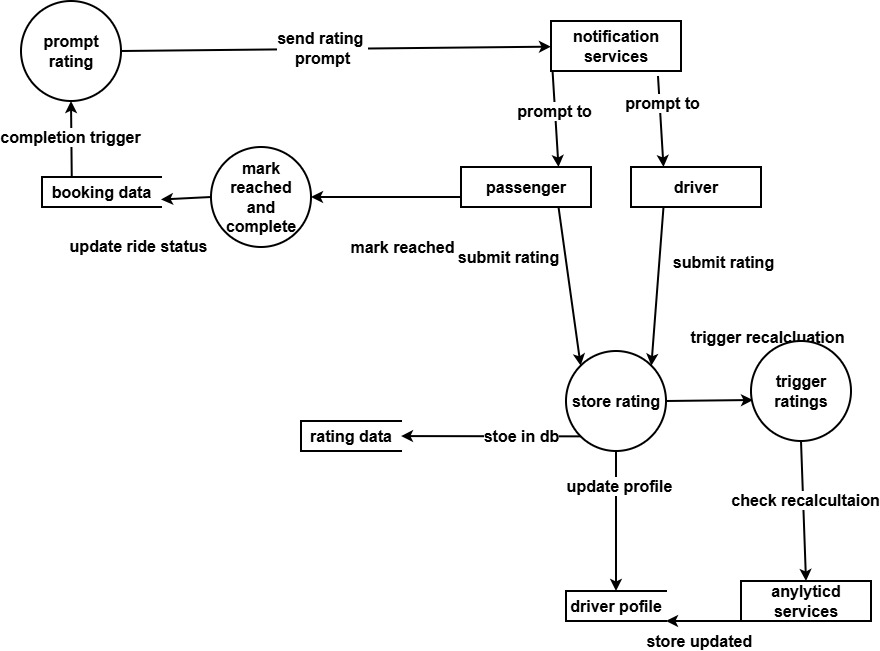
\includegraphics[width=0.9\textwidth,keepaspectratio,height=0.65\textheight]{assets/DFD/module 11 ratings.jpg}
\caption{Level 1 DFD - Ratings and Completion}
\label{fig:dfd_rating}
\vspace{10pt}
\raggedright
\textbf{Processes:} 
\begin{itemize}[noitemsep,topsep=0pt]
    \item Prompt Rating, Submit Rating, Update User Rating, Complete Ride
\end{itemize}
\textbf{Data Stores:} 
\begin{itemize}[noitemsep,topsep=0pt]
    \item Rating DB, Ride DB, User DB
\end{itemize}
\textbf{External Entities:} 
\begin{itemize}[noitemsep,topsep=0pt]
    \item Passenger, Driver
\end{itemize}
\end{figure}

\subsubsection{SOS / Emergency \& Incident Management}

\begin{figure}[H]
\centering
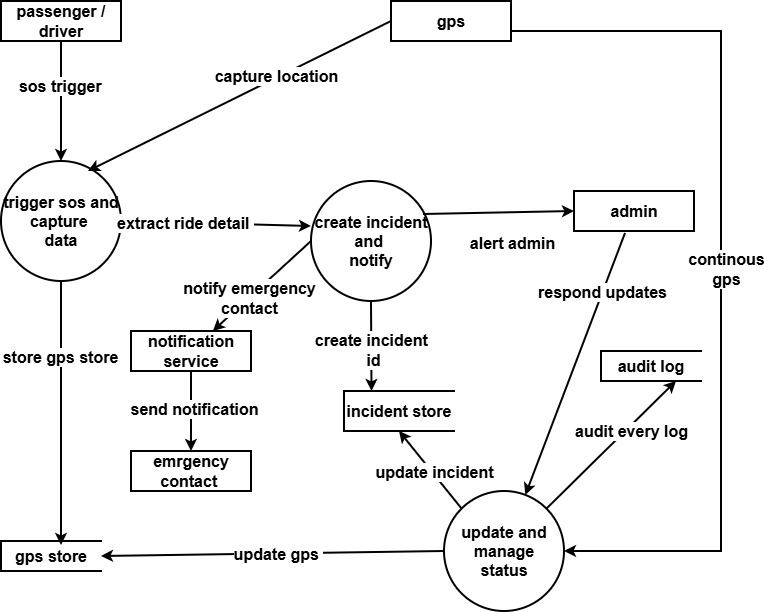
\includegraphics[width=0.9\textwidth,keepaspectratio,height=0.65\textheight]{assets/DFD/module 12.jpg}
\caption{Level 1 DFD - SOS and Emergency Management}
\label{fig:dfd_sos}
\vspace{10pt}
\raggedright
\textbf{Processes:} 
\begin{itemize}[noitemsep,topsep=0pt]
    \item Trigger SOS, Notify Contacts, Notify Admin, Log Incident, Escalate
\end{itemize}
\textbf{Data Stores:} 
\begin{itemize}[noitemsep,topsep=0pt]
    \item SOS DB, User DB, Ride DB
\end{itemize}
\textbf{External Entities:} 
\begin{itemize}[noitemsep,topsep=0pt]
    \item User, Emergency Contact, Admin, Notification Service
\end{itemize}
\end{figure}


\subsubsection{Dispute Management \& Admin Dashboard}

\begin{figure}[H]
\centering
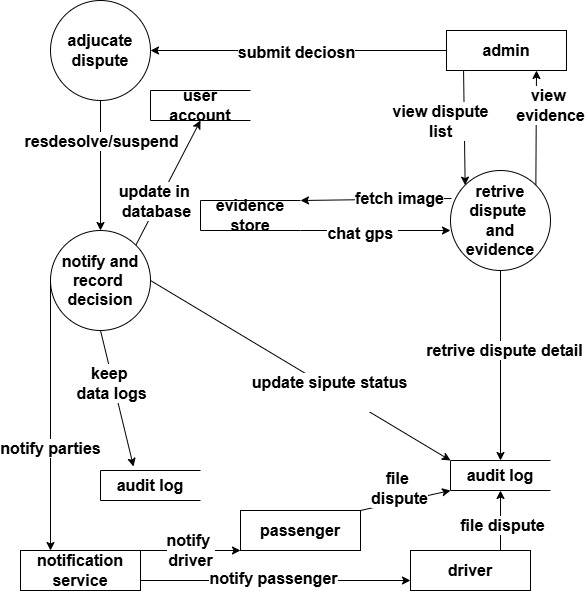
\includegraphics[width=0.9\textwidth,keepaspectratio,height=0.65\textheight]{assets/DFD/module13.jpg}
\caption{Level 1 DFD - Dispute Management}
\label{fig:dfd_dispute}
\vspace{10pt}
\raggedright
\textbf{Processes:} 
\begin{itemize}[noitemsep,topsep=0pt]
    \item File Dispute, View Dispute, Review Evidence, Resolve Dispute, Notify Parties
\end{itemize}
\textbf{Data Stores:} 
\begin{itemize}[noitemsep,topsep=0pt]
    \item Dispute DB, Chat DB, Location DB
\end{itemize}
\textbf{External Entities:} 
\begin{itemize}[noitemsep,topsep=0pt]
    \item User, Admin, Notification Service
\end{itemize}
\end{figure}


\subsubsection{Notification Service}

\begin{figure}[H]
\centering
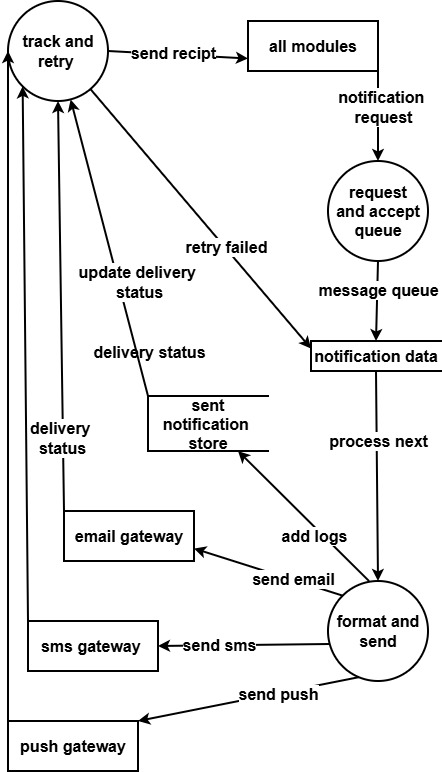
\includegraphics[width=0.9\textwidth,keepaspectratio,height=0.65\textheight]{assets/DFD/module14.jpg}
\caption{Level 1 DFD - Notification Service}
\label{fig:dfd_notification}
\vspace{10pt}
\raggedright
\textbf{Processes:} 
\begin{itemize}[noitemsep,topsep=0pt]
    \item Queue Notification, Send Push, Send SMS, Send Email, Log Delivery
\end{itemize}
\textbf{Data Stores:} 
\begin{itemize}[noitemsep,topsep=0pt]
    \item Notification Log DB
\end{itemize}
\textbf{External Entities:} 
\begin{itemize}[noitemsep,topsep=0pt]
    \item Application, FCM, SMS Gateway, Email Service
\end{itemize}
\end{figure}


\subsubsection{Recommendation (ML) Service}

\begin{figure}[H]
\centering
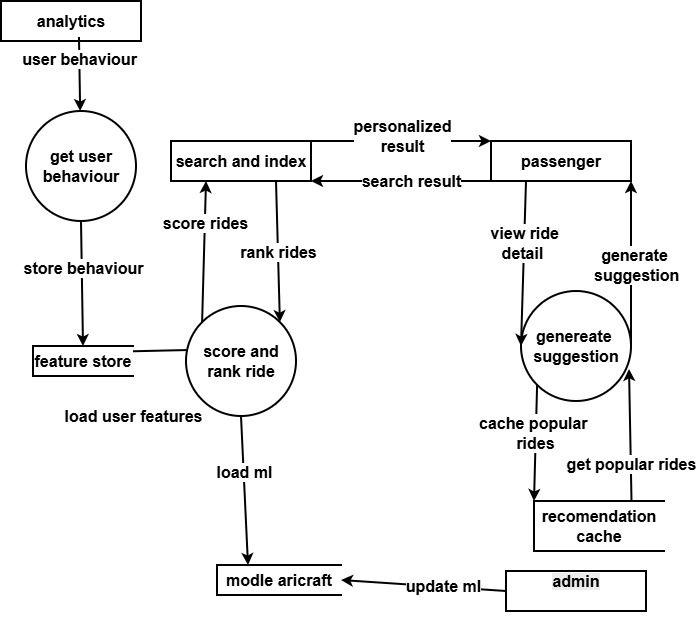
\includegraphics[width=0.9\textwidth,keepaspectratio,height=0.65\textheight]{assets/DFD/module15.jpg}
\caption{Level 1 DFD - ML Recommendation Service}
\label{fig:dfd_ml}
\vspace{10pt}
\raggedright
\textbf{Processes:} 
\begin{itemize}[noitemsep,topsep=0pt]
    \item Fetch User History, Build Feature Vectors, Compute Similarity, Rank Rides
\end{itemize}
\textbf{Data Stores:} 
\begin{itemize}[noitemsep,topsep=0pt]
    \item Ride DB, User History DB
\end{itemize}
\textbf{External Entities:} 
\begin{itemize}[noitemsep,topsep=0pt]
    \item Application, ML Model
\end{itemize}
\end{figure}


\subsubsection{Smart Chatbot Support}

\begin{figure}[H]
\centering
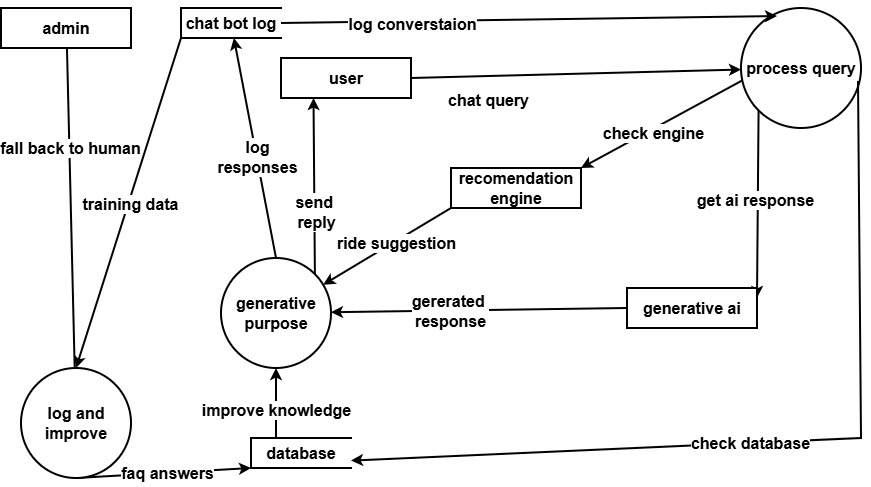
\includegraphics[width=0.9\textwidth,keepaspectratio,height=0.65\textheight]{assets/DFD/module16.jpg}
\caption{Level 1 DFD - Smart Chatbot Support}
\label{fig:dfd_chatbot}
\vspace{10pt}
\raggedright
\textbf{Processes:} 
\begin{itemize}[noitemsep,topsep=0pt]
    \item Parse Query, Classify Intent, Fetch FAQ, Call ML for Recommendations, Format Response
\end{itemize}
\textbf{Data Stores:} 
\begin{itemize}[noitemsep,topsep=0pt]
    \item FAQ KB, Ride DB
\end{itemize}
\textbf{External Entities:} 
\begin{itemize}[noitemsep,topsep=0pt]
    \item User, LLM API, ML Service
\end{itemize}
\end{figure}


\subsubsection{Audit / Logging / Analytics}

\begin{figure}[H]
\centering
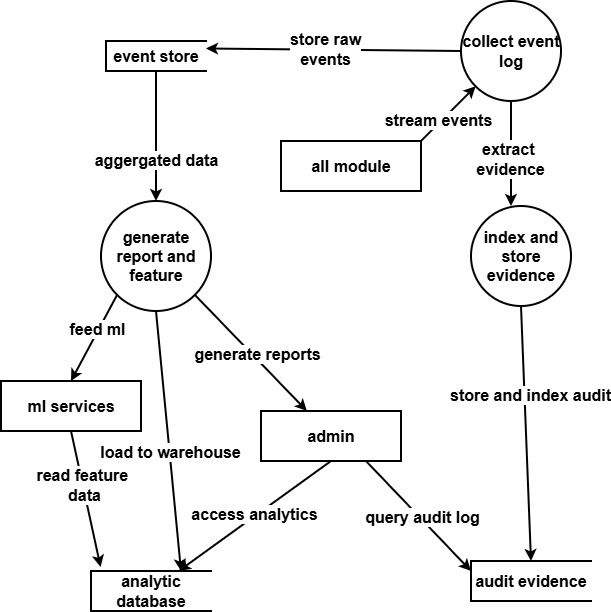
\includegraphics[width=0.9\textwidth,keepaspectratio,height=0.65\textheight]{assets/DFD/module17.jpg}
\caption{Level 1 DFD - Audit, Logging, and Analytics}
\label{fig:dfd_audit}
\vspace{10pt}
\raggedright
\textbf{Processes:} 
\begin{itemize}[noitemsep,topsep=0pt]
    \item Log Event, Store Log, Analyze Patterns, Generate Reports, Detect Fraud
\end{itemize}
\textbf{Data Stores:} 
\begin{itemize}[noitemsep,topsep=0pt]
    \item Audit Log DB
\end{itemize}
\textbf{External Entities:} 
\begin{itemize}[noitemsep,topsep=0pt]
    \item All System Components, Admin
\end{itemize}
\end{figure}

%===========================================================
\section{Data Design}
%===========================================================

This section describes how data is structured, stored, and managed.

\textbf{Guidelines:}
\begin{itemize}
    \item Define database type (SQL / NoSQL).
    \item Explain schema structure.
    \item Describe indexing strategy.
    \item Mention security mechanisms.
    \item Discuss scalability considerations.
\end{itemize}

The Data Design section explains the conversion of the information domain of the Lets Go Ride Sharing App - Ride Sharing and Recommendation System into logical and physical data structures. This contains data entities, relationships, storage plans as well as the entire schema of the database. 

It employs PostgreSQL as the relational database because it is stable, supports indexing, geospatial extensions and highly supports multiple simultaneous transactions, which is required in a ride-sharing system where drivers and riders interact in real-time. 

The data design will have the backend system and the external services dealing with accurate, normalized, and well-structured data.

\subsection{Entity Relationship Diagram (ERD)}

The Entity Relationship Diagram (ERD) represents the logical database structure of the system.

\textbf{Guidelines:}
\begin{itemize}
    \item Clearly identify all entities (tables/collections).
    \item Highlight Primary Keys (PK).
    \item Highlight Foreign Keys (FK).
    \item Show relationship cardinality (1:1, 1:N, M:N).
    \item Maintain consistency with database tables defined earlier.
\end{itemize}

\textbf{Include in ERD:}
\begin{itemize}
    \item \textbf{User Entity}: User (abstract superclass), Passenger, Driver.
    \item \textbf{Core Functional Entities}: RideRequest, Ride, Booking, Location.
    \item \textbf{Transaction/Log Entity}: Payment, Complaint, SOSRequest, ChatMessage.
    \item \textbf{Administrative Entity}: User verification state and user document/image URL fields.
\end{itemize}

\begin{sidewaysfigure}
\centering
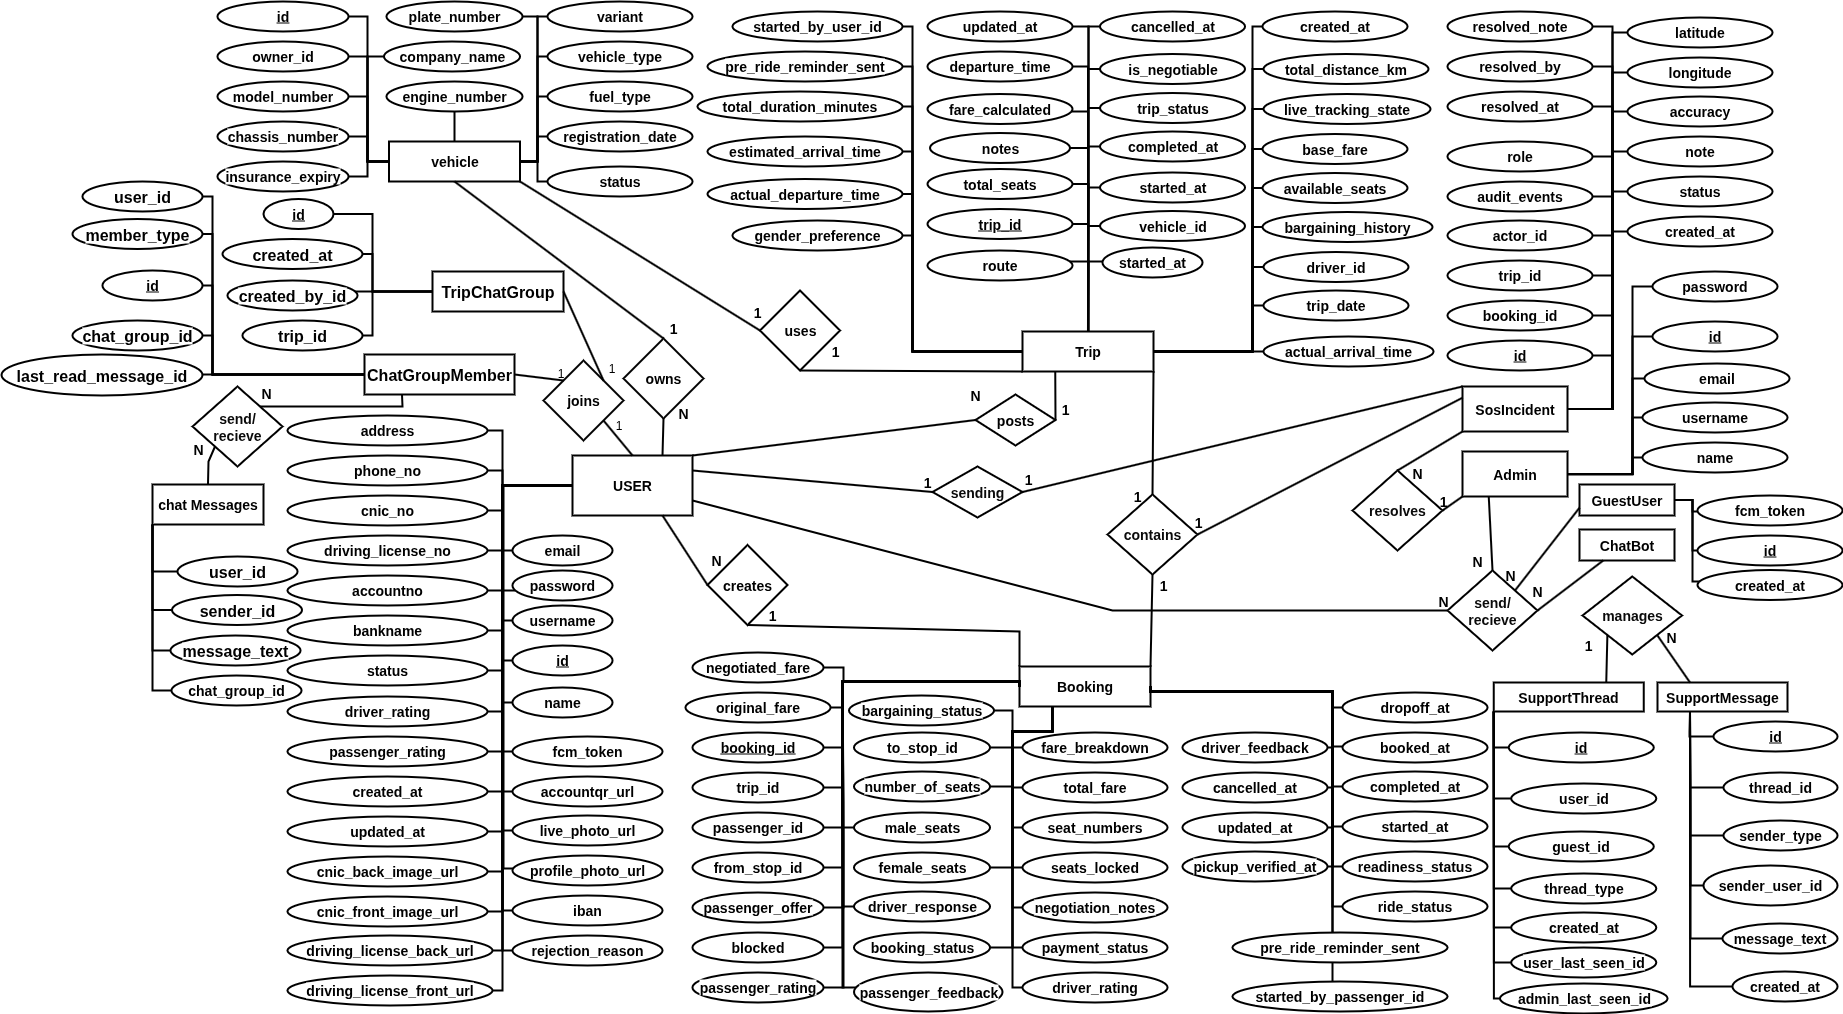
\includegraphics[width=1.0\linewidth,keepaspectratio]{assets/db_diagrams/ERD_DIAGRAMAS.png}
\caption{Entity Relationship Diagram}
\label{fig:erd_diagram}
\end{sidewaysfigure}

\subsection{Database Architecture}

\textbf{Explain:}
\begin{itemize}
    \item \textbf{Client-Server Architecture}: The data in the system are efficiently, safely, and scalably handled through a centralized relational approach.
    \item \textbf{Relational Storage (PostgreSQL)}: Used for User profiles, Rides, bookings, payments, SOS and complaints, Chat messages, and Documents metadata.
    \item \textbf{Geospatial Computation}: Distance calculations and route summaries are handled in application logic using geographic coordinates.
    \item \textbf{Cloud Storage}: Handled via Storage Service for Driver license images, CNIC images, and Profile pictures.
    \item \textbf{Caching Layer}: Optional caching can be applied for frequently accessed read-heavy data when needed.
\end{itemize}

%===========================================================
\section{Database Schema Diagram}
%===========================================================

The physical data model specifies actual database tables, columns, data types, primary keys, foreign keys, and constraints.

The Database Schema Diagram represents the physical database implementation structure.

\textbf{Guidelines:}
\begin{itemize}
    \item Show actual table structure.
    \item Include column names and data types.
    \item Show PK and FK relationships.
    \item Reflect normalization level (1NF, 2NF, 3NF if applicable).
\end{itemize}

\begin{figure}[H]
\centering
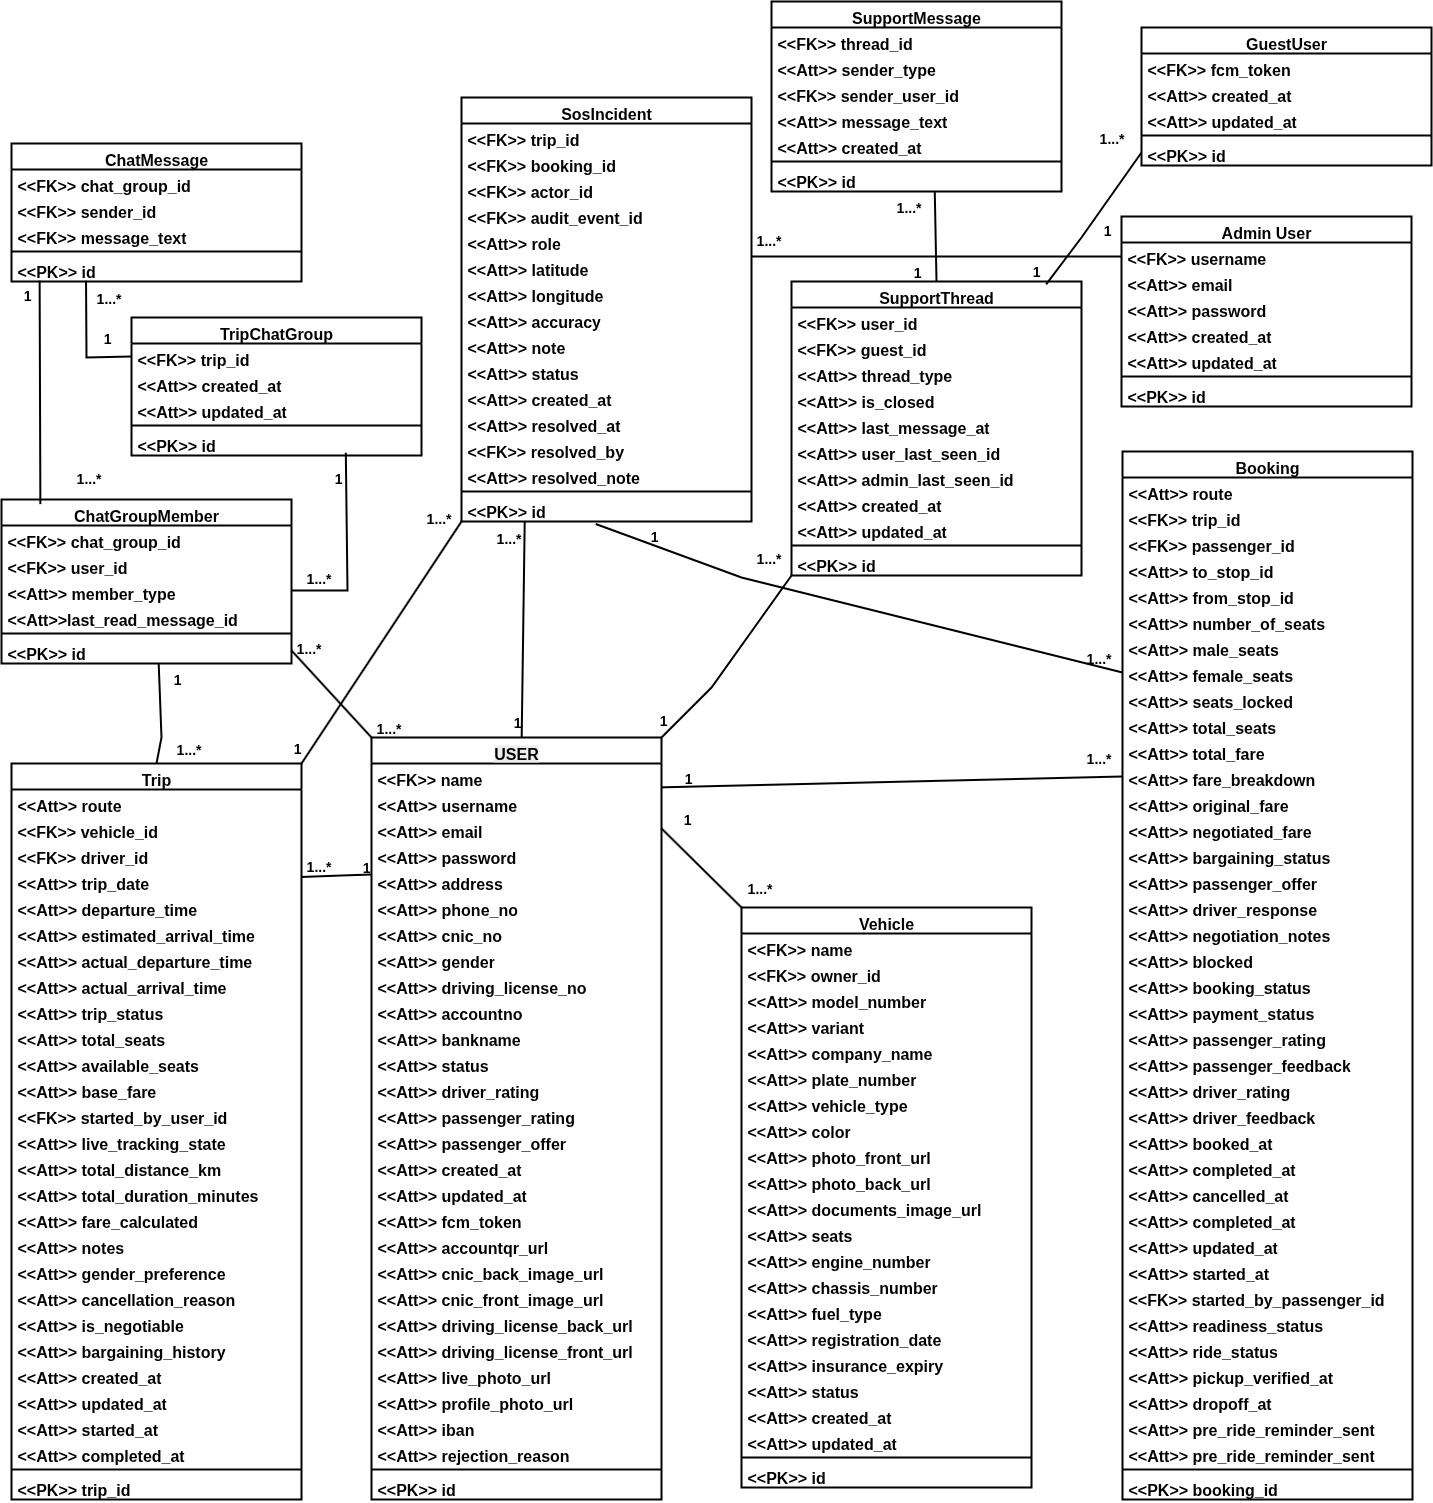
\includegraphics[width=0.9\textwidth,keepaspectratio,height=0.8\textheight]{assets/db_diagrams/DB_SCHEM.png}
\caption{Physical Database Schema Diagram showing table structures and relationships}
\label{fig:schema}
\end{figure}

The database schema is normalized to 3NF to eliminate Data redundancy. This structured design ensures \textbf{data integrity} by enforcing strict relational constraints (Foreign Keys) between tables like Users, Rides, and Bookings. It supports \textbf{efficient querying} through indexing on frequently accessed fields like \texttt{user\_id} and \texttt{ride\_id}. The schema's modularity allows \textbf{scalability} by enabling seamless extension of tables without affecting core operations. Finally, \textbf{security} is maintained by isolating sensitive authentication data in the core User table away from public operational data.

\subsection{Data Dictionary}

The Data Dictionary defines the structure of all primary data elements in the database.

\textbf{Guidelines:}
\begin{itemize}
    \item Include field name, Data type, Size, Description, Constraints.
\end{itemize}

\begin{table}[H]
\centering
\caption{Data Dictionary – Booking Table}
\renewcommand{\arraystretch}{1.5}
\begin{tabular}{|p{3cm}|p{3cm}|p{7cm}|}
\hline
\textbf{Attribute} & \textbf{Type} & \textbf{Description} \\
\hline
booking\_id & CharField & Unique booking identifier (PK) \\
\hline
trip & ForeignKey & Associated Trip (FK to Trip) \\
\hline
passenger & ForeignKey & Associated Passenger (FK to UsersData) \\
\hline
from\_stop & ForeignKey & Pickup stop (FK to RouteStop) \\
\hline
to\_stop & ForeignKey & Drop-off stop (FK to RouteStop) \\
\hline
number\_of\_seats & Integer & Total seats booked for this request \\
\hline
male\_seats & Integer & Number of seats for male passengers \\
\hline
female\_seats & Integer & Number of seats for female passengers \\
\hline
total\_fare & Integer & Total fare for the booking \\
\hline
booking\_status & CharField & Current status (PENDING, CONFIRMED, etc.) \\
\hline
payment\_status & CharField & Payment status (PENDING, COMPLETED, etc.) \\
\hline
\end{tabular}
\end{table}

\begin{table}[H]
\centering
\caption{Data Dictionary – ChatMessage Table}
\renewcommand{\arraystretch}{1.5}
\begin{tabular}{|p{3cm}|p{3cm}|p{7cm}|}
\hline
\textbf{Attribute} & \textbf{Type} & \textbf{Description} \\
\hline
id & AutoField & Unique message identifier (PK) \\
\hline
chat\_group & ForeignKey & Associated chat group (FK to TripChatGroup) \\
\hline
sender & ForeignKey & User who sent the message (FK to UsersData) \\
\hline
message\_type & CharField & Type of message (TEXT, IMAGE, SYSTEM) \\
\hline
message\_text & TextField & Content of the message \\
\hline
created\_at & DateTime & Timestamp when message was sent \\
\hline
is\_deleted & Boolean & Flag for deleted messages \\
\hline
\end{tabular}
\end{table}

\begin{table}[H]
\centering
\caption{Data Dictionary – SosIncident Table}
\renewcommand{\arraystretch}{1.5}
\begin{tabular}{|p{3cm}|p{3cm}|p{7cm}|}
\hline
\textbf{Attribute} & \textbf{Type} & \textbf{Description} \\
\hline
id & AutoField & Unique incident identifier (PK) \\
\hline
trip & ForeignKey & Associated trip (FK to Trip) \\
\hline
actor & ForeignKey & Person who triggered SOS (FK to UsersData) \\
\hline
role & CharField & Role of the actor (Passenger/Driver) \\
\hline
latitude & Decimal & GPS latitude at trigger time \\
\hline
longitude & Decimal & GPS longitude at trigger time \\
\hline
status & CharField & Current status (OPEN, RESOLVED) \\
\hline
created\_at & DateTime & Time incident was recorded \\
\hline
\end{tabular}
\end{table}

\begin{table}[H]
\centering
\caption{Data Dictionary – Driver Fields in UsersData}
\renewcommand{\arraystretch}{1.5}
\begin{tabular}{|p{3cm}|p{3cm}|p{7cm}|}
\hline
\textbf{Attribute} & \textbf{Type} & \textbf{Description} \\
\hline
driving\_license\_no & CharField & National driving license identification \\
\hline
driving\_license\_front\_url & URLField & Link to license front image \\
\hline
driving\_license\_back\_url & URLField & Link to license back image \\
\hline
driver\_rating & Decimal & Average rating as a driver \\
\hline
status & CharField & Verification status (PENDING, VERIFIED) \\
\hline
bankname & CharField & Name of driver's bank for payments \\
\hline
iban & CharField & Bank account IBAN for transfers \\
\hline
\end{tabular}
\end{table}

\begin{table}[H]
\centering
\caption{Data Dictionary – TripLiveLocationUpdate Table}
\renewcommand{\arraystretch}{1.5}
\begin{tabular}{|p{3cm}|p{3cm}|p{7cm}|}
\hline
\textbf{Attribute} & \textbf{Type} & \textbf{Description} \\
\hline
trip & ForeignKey & Associated trip (FK to Trip) \\
\hline
user & ForeignKey & User providing update (FK to UsersData) \\
\hline
latitude & Decimal & Current latitude coordinate \\
\hline
longitude & Decimal & Current longitude coordinate \\
\hline
speed\_mps & Float & Speed in meters per second \\
\hline
recorded\_at & DateTime & Timestamp of the location update \\
\hline
\end{tabular}
\end{table}

\begin{table}[H]
\centering
\caption{Data Dictionary – Passenger Fields in UsersData}
\renewcommand{\arraystretch}{1.5}
\begin{tabular}{|p{3cm}|p{3cm}|p{7cm}|}
\hline
\textbf{Attribute} & \textbf{Type} & \textbf{Description} \\
\hline
passenger\_rating & Decimal & Average rating as a passenger \\
\hline
fcm\_token & TextField & Push notification token \\
\hline
address & TextField & Primary residence address \\
\hline
phone\_no & CharField & Contact number \\
\hline
name & CharField & Full legal name \\
\hline
\end{tabular}
\end{table}

\begin{table}[H]
\centering
\caption{Data Dictionary – TripPayment Table}
\renewcommand{\arraystretch}{1.5}
\begin{tabular}{|p{3cm}|p{3cm}|p{7cm}|}
\hline
\textbf{Attribute} & \textbf{Type} & \textbf{Description} \\
\hline
booking & ForeignKey & Associated booking (FK to Booking) \\
\hline
payment\_method & CharField & Method (CASH, BANK\_TRANSFER, etc.) \\
\hline
amount & Integer & Payment amount paid in PKR \\
\hline
transaction\_id & CharField & Unique external transaction reference \\
\hline
payment\_status & CharField & Status (PENDING, COMPLETED, FAILED) \\
\hline
created\_at & DateTime & Time when payment was initiated \\
\hline
\end{tabular}
\end{table}

\begin{table}[H]
\centering
\caption{Data Dictionary – Trip Table}
\renewcommand{\arraystretch}{1.5}
\begin{tabular}{|p{3cm}|p{3cm}|p{7cm}|}
\hline
\textbf{Attribute} & \textbf{Type} & \textbf{Description} \\
\hline
trip\_id & CharField & Unique trip identifier (PK) \\
\hline
route & ForeignKey & Associated route (FK to Route) \\
\hline
vehicle & ForeignKey & Assigned vehicle (FK to Vehicle) \\
\hline
driver & ForeignKey & Assigned driver (FK to UsersData) \\
\hline
trip\_date & DateField & Date of the scheduled trip \\
\hline
departure\_time & TimeField & Scheduled start time \\
\hline
trip\_status & CharField & Status (SCHEDULED, IN\_PROGRESS, etc.) \\
\hline
available\_seats & Integer & Remaining seats for booking \\
\hline
base\_fare & Integer & Standard fare for the trip \\
\hline
\end{tabular}
\end{table}

\begin{table}[H]
\centering
\caption{Data Dictionary – Route Table}
\renewcommand{\arraystretch}{1.5}
\begin{tabular}{|p{3cm}|p{3cm}|p{7cm}|}
\hline
\textbf{Attribute} & \textbf{Type} & \textbf{Description} \\
\hline
route\_id & CharField & Unique route code (e.g., R001) (PK) \\
\hline
route\_name & CharField & Descriptive name for the route \\
\hline
total\_distance\_km & Decimal & Total length of the route \\
\hline
estimated\_duration & Integer & Estimated travel time in minutes \\
\hline
route\_geometry & JSONField & List of GPS points for map rendering \\
\hline
is\_active & Boolean & Whether the route is currently operational \\
\hline
\end{tabular}
\end{table}

\begin{table}[H]
\centering
\caption{Data Dictionary – EmergencyContact Table}
\renewcommand{\arraystretch}{1.5}
\begin{tabular}{|p{3cm}|p{3cm}|p{7cm}|}
\hline
\textbf{Attribute} & \textbf{Type} & \textbf{Description} \\
\hline
user & OneToOneField & Associated user (FK to UsersData) \\
\hline
name & CharField & Contact person's name \\
\hline
relation & CharField & Relationship to user (e.g., Father, Friend) \\
\hline
phone\_no & CharField & Emergency contact phone number \\
\hline
email & EmailField & Emergency contact email address \\
\hline
\end{tabular}
\end{table}

\begin{table}[H]
\centering
\caption{Data Dictionary – UsersData Table}
\renewcommand{\arraystretch}{1.5}
\begin{tabular}{|p{3cm}|p{3.5cm}|p{6.5cm}|}
\hline
\textbf{Attribute} & \textbf{Type} & \textbf{Description} \\
\hline
id & AutoField & Unique user record ID (PK) \\
\hline
username & CharField & Unique login username \\
\hline
email & EmailField & Unique registered email address \\
\hline
password & CharField & Hashed password string \\
\hline
cnic\_no & CharField & Identity card number (XXXXX-XXXXXXX-X) \\
\hline
gender & CharField & male, female \\
\hline
status & CharField & PENDING, VERIFIED, BANNED \\
\hline
created\_at & DateTime & Signup timestamp \\
\hline
\end{tabular}
\end{table}

\begin{table}[H]
\centering
\caption{Data Dictionary – Vehicle Table}
\renewcommand{\arraystretch}{1.5}
\begin{tabular}{|p{3cm}|p{3cm}|p{7cm}|}
\hline
\textbf{Attribute} & \textbf{Type} & \textbf{Description} \\
\hline
id & AutoField & Unique vehicle identifier (PK) \\
\hline
owner & ForeignKey & Driver owning vehicle (FK to UsersData) \\
\hline
model\_number & CharField & Vehicle model (e.g., Corolla 2022) \\
\hline
plate\_number & CharField & Unique license plate number \\
\hline
vehicle\_type & CharField & TW (Two Wheeler), FW (Four Wheeler) \\
\hline
seats & Integer & Number of passenger seats \\
\hline
fuel\_type & CharField & Petrol, Diesel, CNG, etc. \\
\hline
status & CharField & VERIFIED, PENDING, REJECTED \\
\hline
\end{tabular}
\end{table}

\begin{table}[H]
\centering
\caption{Data Dictionary – RouteStop Table}
\renewcommand{\arraystretch}{1.5}
\begin{tabular}{|p{3cm}|p{3cm}|p{7cm}|}
\hline
\textbf{Attribute} & \textbf{Type} & \textbf{Description} \\
\hline
route & ForeignKey & Parent route (FK to Route) \\
\hline
stop\_name & CharField & Name of the stop/pickup point \\
\hline
stop\_order & Integer & Sequence of the stop in the route \\
\hline
latitude & Decimal & GPS latitude for the stop \\
\hline
longitude & Decimal & GPS longitude for the stop \\
\hline
address & TextField & Detailed address of the stop \\
\hline
\end{tabular}
\end{table}

%===========================================================
\section{Database Tables / Collections}
%===========================================================

This section describes the logical database design of the system. It presents the major relational tables (for SQL-based systems) or collections (for NoSQL-based systems). The database structure is designed to ensure data consistency, integrity, security, and scalability.

Each table or collection includes primary keys, relationships, and major attributes relevant to system functionality.

\subsection{User Collection / Table}

The User table stores authentication credentials and user profile information. It supports role-based access control and secure authentication.

\textbf{Description:}
\begin{itemize}
    \item \textbf{Primary Key:} user\_id
    \item \textbf{Relationships:} Linked to transactions, predictions, or system logs.
    \item \textbf{Authentication Attributes:} Email, password hash, role, account status.
\end{itemize}

\begin{table}[H]
\centering
\caption{UsersData Table Structure}
\renewcommand{\arraystretch}{1.5}
\begin{tabular}{|p{3cm}|p{3.5cm}|p{3cm}|p{5cm}|}
\hline
\textbf{Field Name} & \textbf{Data Type} & \textbf{Constraint} & \textbf{Description} \\
\hline
id & AutoField & Primary Key & Unique identifier for each user \\
\hline
name & VARCHAR(100) & Not Null & User's full name \\
\hline
username & VARCHAR(100) & Unique, Not Null & Unique login username \\
\hline
email & EmailField & Unique, Not Null & Registered email address \\
\hline
password & VARCHAR(128) & MinLength(8) & Hashed password string \\
\hline
cnic\_no & VARCHAR(15) & Unique, Regex & Identity card number \\
\hline
status & VARCHAR(10) & Choice & Enum: PENDING, VERIFIED, BANNED \\
\hline
\end{tabular}
\end{table}

\subsection{Core Data Collection}

This subsection describes domain-specific core data tables. These structures store the primary operational data processed by the Ride Booking system.

\textbf{Domain-Specific Tables:}

\subsubsection{Passenger Data (UsersData)}
\begin{table}[H]
\centering
\caption{Passenger-Specific Table Fields}
\renewcommand{\arraystretch}{1.5}
\begin{tabular}{|p{3cm}|p{3.5cm}|p{7cm}|}
\hline
\textbf{Field Name} & \textbf{Data Type} & \textbf{Description} \\
\hline
passenger\_rating & DecimalField & Average rating from drivers \\
\hline
address & TextField & Pickup/Home address \\
\hline
phone\_no & CharField & Contact number with validation \\
\hline
fcm\_token & TextField & Firebase notification token \\
\hline
\end{tabular}
\end{table}

\subsubsection{Driver Data (UsersData)}
\begin{table}[H]
\centering
\caption{Driver-Specific Table Fields}
\renewcommand{\arraystretch}{1.5}
\begin{tabular}{|p{3cm}|p{3.5cm}|p{7cm}|}
\hline
\textbf{Field Name} & \textbf{Data Type} & \textbf{Description} \\
\hline
driving\_license\_no & CharField & Professional license number \\
\hline
driving\_license\_front\_url & URLField & Image of license front \\
\hline
bankname & CharField & Transaction bank name \\
\hline
iban & CharField & International Bank Account Number \\
\hline
driver\_rating & DecimalField & Average rating from passengers \\
\hline
\end{tabular}
\end{table}

\subsubsection{Vehicle Table}
\begin{table}[H]
\centering
\caption{Vehicle Table}
\renewcommand{\arraystretch}{1.5}
\begin{tabular}{|p{3cm}|p{3.5cm}|p{7cm}|}
\hline
\textbf{Field Name} & \textbf{Data Type} & \textbf{Description} \\
\hline
id (PK) & AutoField & Unique database ID \\
\hline
owner (FK) & ForeignKey & Link to UsersData (Owner) \\
\hline
model\_number & CharField & Vehicle specific model \\
\hline
plate\_number & CharField & UNIQUE registration plate \\
\hline
vehicle\_type & CharField & Choices: TW or FW \\
\hline
seats & PositiveInt & Available seating capacity \\
\hline
fuel\_type & CharField & Petrol, Diesel, CNG, etc. \\
\hline
\end{tabular}
\end{table}

\subsubsection{Route Table}
\begin{table}[H]
\centering
\caption{Route Table}
\renewcommand{\arraystretch}{1.5}
\begin{tabular}{|p{3cm}|p{3.5cm}|p{7cm}|}
\hline
\textbf{Field Name} & \textbf{Data Type} & \textbf{Description} \\
\hline
route\_id & CharField & Unique identifier (e.g., R001) \\
\hline
route\_name & CharField & Name of the route \\
\hline
total\_distance\_km & DecimalField & Length of trip in km \\
\hline
estimated\_duration & IntegerField & Duration in minutes \\
\hline
route\_geometry & JSONField & Polylines for map display \\
\hline
is\_active & BooleanField & Status of the route \\
\hline
\end{tabular}
\end{table}

\subsubsection{Booking Table}
\begin{table}[H]
\centering
\caption{Booking Table}
\renewcommand{\arraystretch}{1.5}
\begin{tabular}{|p{3cm}|p{3.5cm}|p{7cm}|}
\hline
\textbf{Field Name} & \textbf{Data Type} & \textbf{Description} \\
\hline
booking\_id (PK) & CharField & Unique Booking identifier \\
\hline
trip (FK) & ForeignKey & Link to Trip record \\
\hline
passenger (FK) & ForeignKey & Link to UsersData record \\
\hline
number\_of\_seats & IntegerField & Seats requested \\
\hline
total\_fare & IntegerField & Final calculated cost \\
\hline
booking\_status & CharField & PENDING, CONFIRMED, etc. \\
\hline
payment\_status & CharField & Payment state \\
\hline
\end{tabular}
\end{table}

\subsubsection{Trip Table}
\begin{table}[H]
\centering
\caption{Trip Table}
\renewcommand{\arraystretch}{1.5}
\begin{tabular}{|p{3cm}|p{3.5cm}|p{7cm}|}
\hline
\textbf{Field Name} & \textbf{Data Type} & \textbf{Description} \\
\hline
trip\_id (PK) & CharField & Unique Trip identifier \\
\hline
route (FK) & ForeignKey & FK to Route model \\
\hline
vehicle (FK) & ForeignKey & FK to Vehicle model \\
\hline
driver (FK) & ForeignKey & FK to UsersData model \\
\hline
trip\_date & DateField & Date of travel \\
\hline
trip\_status & CharField & SCHEDULED, COMPLETED, etc. \\
\hline
available\_seats & IntegerField & Current capacity left \\
\hline
\end{tabular}
\end{table}

\subsubsection{TripPayment Table}
\begin{table}[H]
\centering
\caption{TripPayment Table}
\renewcommand{\arraystretch}{1.5}
\begin{tabular}{|p{3cm}|p{3.5cm}|p{7cm}|}
\hline
\textbf{Field Name} & \textbf{Data Type} & \textbf{Description} \\
\hline
id (PK) & AutoField & Unique Payment ID \\
\hline
booking (FK) & ForeignKey & FK to Booking model \\
\hline
payment\_method & CharField & CASH, BANK\_TRANSFER, etc. \\
\hline
amount & IntegerField & Fare amount in PKR \\
\hline
payment\_status & CharField & PENDING, COMPLETED, etc. \\
\hline
created\_at & DateTimeField & Initial timestamp \\
\hline
\end{tabular}
\end{table}

\subsubsection{SosIncident Table}
\begin{table}[H]
\centering
\caption{SosIncident Table}
\renewcommand{\arraystretch}{1.5}
\begin{tabular}{|p{3cm}|p{3.5cm}|p{7cm}|}
\hline
\textbf{Field Name} & \textbf{Data Type} & \textbf{Description} \\
\hline
id (PK) & AutoField & Unique SOS entry \\
\hline
trip (FK) & ForeignKey & FK to Trip model \\
\hline
actor (FK) & ForeignKey & Link to triggering User \\
\hline
role & CharField & Role (Passenger/Driver) \\
\hline
status & CharField & OPEN or RESOLVED \\
\hline
created\_at & DateTimeField & Time of trigger \\
\hline
\end{tabular}
\end{table}

\subsubsection{EmergencyContact Table}
\begin{table}[H]
\centering
\caption{EmergencyContact Table}
\renewcommand{\arraystretch}{1.5}
\begin{tabular}{|p{3cm}|p{3.5cm}|p{7cm}|}
\hline
\textbf{Field Name} & \textbf{Data Type} & \textbf{Description} \\
\hline
user (FK) & OneToOneField & Link to UsersData \\
\hline
name & CharField & Contact name \\
\hline
phone\_no & CharField & Verified contact number \\
\hline
relation & CharField & Relationship to user \\
\hline
\end{tabular}
\end{table}

\subsubsection{ChatMessage Table}
\begin{table}[H]
\centering
\caption{ChatMessage Table}
\renewcommand{\arraystretch}{1.5}
\begin{tabular}{|p{3cm}|p{3.5cm}|p{7cm}|}
\hline
\textbf{Field Name} & \textbf{Data Type} & \textbf{Description} \\
\hline
id (PK) & AutoField & Message primary key \\
\hline
chat\_group (FK) & ForeignKey & FK to TripChatGroup \\
\hline
sender (FK) & ForeignKey & FK to UsersData \\
\hline
message\_type & CharField & TEXT, IMAGE, SYSTEM \\
\hline
message\_text & TextField & Encrypted text content \\
\hline
\end{tabular}
\end{table}

\subsection{Relationships Between Tables}

Database relationships define how data entities are connected within the Lets Go Ride Sharing App system.

\begin{itemize}
    \item \textbf{One Driver $\rightarrow$ Many Vehicles} (1-to-M)
    \item \textbf{One Passenger $\rightarrow$ Many Bookings} (1-to-M)
    \item \textbf{Many Bookings $\rightarrow$ One Trip} (M-to-1)
    \item \textbf{One Booking $\rightarrow$ One Payment} (1-to-1)
    \item \textbf{One Trip $\rightarrow$ Many SosIncidents} (1-to-M)
    \item \textbf{One User $\rightarrow$ One EmergencyContact} (1-to-1)
    \item \textbf{One Trip $\rightarrow$ One ChatGroup} (1-to-1)
    \item \textbf{One ChatGroup $\rightarrow$ Many ChatMessages} (1-to-M)
\end{itemize}

An Entity-Relationship (ER) Diagram visually represents these relationships.

\subsection{Security and Data Integrity}

To ensure confidentiality and integrity of stored data, the following measures are implemented:
\begin{itemize}
    \item \textbf{Password Encryption} using secure hashing algorithms (e.g., bcrypt, SHA-256 with salt).
    \item \textbf{Role-Based Access Control (RBAC)} to restrict unauthorized access between passengers, drivers, and admins.
    \item \textbf{Input validation} and constraint enforcement at the database level (e.g., NOT NULL, UNIQUE constraints).
    \item \textbf{Secure communication} using HTTPS for API endpoints accessing the DB.
    \item \textbf{Regular database backup} and disaster recovery strategy.
\end{itemize}

\subsection{Scalability Considerations}

The database design incorporates scalability mechanisms to support future growth of the ride-sharing platform.
\begin{itemize}
    \item \textbf{Horizontal Scaling} using distributed database systems.
    \item \textbf{Indexing} on frequently queried attributes (like \texttt{pickup\_location}, \texttt{drop\_location}, \texttt{status}) to improve search performance.
    \item \textbf{Caching strategies} for frequently accessed data like active ride and booking summaries.
    \item \textbf{Load balancing} across database instances for API request handling.
    \item \textbf{Partitioning or sharding} for large-scale data environments (e.g., partitioning old ride records by year).
\end{itemize}

%===========================================================
\section{Chapter Summary}
%===========================================================

This chapter discussed the software architecture and design of the Let’s Go system in detail. It outlined the transition from requirements to an actual system blueprint using an Agile incremental model. 

Key modeling diagrams—including Activity, Class, Sequence, and State Transition diagrams—were presented to illustrate the dynamic and structural behavior of the system. Data Flow Diagrams (DFDs) detailed the movement of data across various operational phases, from authentication to ride tracking and dispute resolution. 

The chapter concluded with a comprehensive data design section, explicitly defining PostgreSQL schemas, ER diagrams, data dictionaries, and database relationships to ensure a scalable, secure, and normalized data architecture.
% ============================================
% Chapter 5 – Implementation
% ============================================

\chapter{Implementation}
\justifying

This chapter describes the practical implementation of the Lets Go Ride Sharing App ride-sharing and recommendation system. It explains how the architectural design and models presented in Chapter 4 were translated into working modules, algorithms, user interfaces, and deployment components. The implementation follows the modular design and incremental delivery approach outlined earlier.

% -------------------------------------------------
% 5.1 Development Environment
% -------------------------------------------------

\section{Development Environment}

The development environment for the Lets Go Ride Sharing App system was selected to support Flutter mobile development, a Django backend, PostgreSQL database management, and template-based Admin pages.

\textbf{IDE and Tools:}

Visual Studio Code – main editor for writing Flutter (Dart) and Django (Python).

Android Studio – for Android emulator testing and Flutter layout debugging.

Figma – UI/UX Design \& Prototyping.

Postman – HTTP Endpoint Testing for Backend Integration Testing.
\begin{itemize}
    \item Git \& GitHub – Version control and collaboration (including issue tracking).
\end{itemize}
Supabase Dashboard – Database Inspection and Storage Bucket Management for Supabase PostgreSQL and Supabase Storage.

Programming Languages and Frameworks:

Frontend (Mobile): Dart and Flutter for cross-platform mobile screens.
\begin{itemize}
    \item Frontend: HTML, CSS, and JavaScript.
    \item Database: SQLite.
    \item Authentication: Session-based authentication with Django sessions with the user id saved in the \texttt{request.session['user\_id']} property.
    \item Notifications: Notification logic for the backend and push delivery via FCM as well as email/SMS support where set up.
\end{itemize}
Database: PostgreSQL on Supabase.
\begin{itemize}
    \item Storage: Uploaded images and documents are stored in Supabase Storage.
    \item Haversine Distance: An algorithmic formula for calculating distances between two locations.
\end{itemize}

Backend support chatbot as a local utility within the Django project that can optionally include LLM support in the event that environment variables are set.

Operating System and Hardware:

Development OS: Ubuntu, Windows 10 and Windows 11 have been used for development and testing.
\begin{itemize}
    \item Backend Hosting Environment: Cloud deployment of backend and Admin pages (Django).
    \item Hardware:
        \begin{itemize}
            \item Modern multi-core processor and 16+ GB RAM machines for development.
            \item Application validation (Android and iOS) using mobile test devices and emulators.
        \end{itemize}
\end{itemize}

% -------------------------------------------------
% 5.2 Core Module Implementation
% -------------------------------------------------

\section{Core Module Implementation}

This section describes the implementation of the main modules of the Lets Go Ride Sharing App system. Each module was designed as a standalone feature or a screen flow within the Flutter app, maintaining the code structure and making it easier to maintain.

\subsection{Module 1: Authentication \& Verification Module}

This is used to manage user registration, login, OTP verification, password reset and Admin review of documents.

\textbf{Key Functionalities:}
\begin{itemize}
    \item User Registration by email, phone, CNIC and (optional) license/bank details.
    \item Upload profile images, CNIC images, driver license images, vehicle documents to Supabase Storage.
    \item OTP generation and verification for account verification \& password reset flow.
    \item Logging in automatically to the session once successful.
    \item Administrator pages to see pending validations and approve, reject or ban users.
\end{itemize}

\textbf{Important Classes/Functions:}
\begin{itemize}
    \item User profile database for passenger \& driver data.
    \item User document/image fields stored in user profile model, uploaded assets stored in Supabase Storage with reference through stored URLs.
    \item Web-based helpers for generating and verifying OTPs, with server side cache/state and configured delivery utilities for email/SMS.
    \item Django function-based views were mapped on the following routes: \texttt{/signup/}, \texttt{/login/}, \texttt{/send\_otp/}, \texttt{/verify\_otp/}, and \texttt{/reset\_password/}.
    \item The Flutter screens that are being registered are \texttt{RegistrationScreen}, \texttt{OTPScreen} and \texttt{DocumentUploadScreen}.
\end{itemize}

\textbf{Integration:} interacts with the notification layer for OTP delivery and Supabase Storage for document uploads. The updating of the user status and triggering of the corresponding notifications are carried out due to admin actions.

\subsection{Module 2: Ride Management Module}

\textbf{Aim:} To allow drivers to develop, edit and publish rides as well as control stops on the ride and ride parameters.

\textbf{Key Functionalities:}
\begin{itemize}
    \item Map-based route editor with the ability to create start, intermediate and end stops.
    \item The fare calculation is done based on the distance of the route, type of the vehicle and ride parameters.
    \item Availability of departure time and seats, gender preference and the availability for negotiation.
    \item Adding the ride to the passenger discovery pages and updating the ride information using a form in the backend.
\end{itemize}

\textbf{Important Classes/Functions:}
\begin{itemize}
    \item Ride model using route and stop data.
    \item FareCalculator is a utility to calculate the fare distance, based on Haversine distance, and route metadata.
    \item Django views in \texttt{/create\_route/}, \texttt{/create\_trip/}, and \texttt{/trips/<trip\_id>/...}.
    \item These screens should be flutter screens that are created as follows: \texttt{CreateRideScreen}, \texttt{MyRidesScreen}, and \texttt{RideDetailsScreen}.
\end{itemize}

\textbf{Integration:} Saves data for rides in PostgreSQL, provides fare calculation helpers for routes and distance, and provides access to the ride data to the passenger search and booking flows.

\subsection{Module 3: Booking \& Payment Module}

\textbf{Objective:} To enable passengers to locate, check, reserve and confirm trips, as well as to lock the seats, negotiate and manually confirm payments.

\textbf{Key Functionalities:}
\begin{itemize}
    \item Search for rides by origin, destination, date and gender preference.
    \item Choose pick up and drop off stops from a driver route.
    \item Prevent overbooking by locking seats when booking.
    \item Accept, reject, cancel and confirm bookings.
    \item Manual payment flow in which the passenger indicates that payment is made and the driver checks it.
\end{itemize}

\textbf{Important Classes/Functions:}
\begin{itemize}
    \item Requested, accepted, rejected, cancelled, completed booking model with states.
    \item Payment model that is based on bookings.
    \item Endpoints that are related to Django, like \texttt{/ride-booking/<trip\_id>/}, \texttt{/bookings/<booking\_id>/payment/submit/}, and \texttt{/bookings/<booking\_id>/payment/confirm/}.
    \item The following screens will be fluttered: \texttt{SearchRidesScreen}, \texttt{BookingScreen} and \texttt{PaymentScreen}.
\end{itemize}

\textbf{Integration:} Communicates with notification layer for alerts and updates on state changes after booking rides.

\subsection{Module 4: Live Tracking \& Safety Module}

In this Module 4: Live Tracking \& Safety Module, you will learn how to track animals in the field and how to keep them safe and sound.

\textbf{Purpose:} Frequency update support with HTTP near real-time ride tracking, pickup code verification, SOS emergency and ride completion support.

\textbf{Key Functionalities:}
\begin{itemize}
    \item Location updates are transmitted via HTTP endpoints on the client via polling or periodic updates.
    \item Passenger boarding is verified by code picking and code verification.
    \item SOS incidents alert through e-mail/SMS workflows and create shareable tracking links or tokens.
    \item Data of the incidents and tracking data are saved for review in the Admin pages.
\end{itemize}

\textbf{Important Classes/Functions:}
\begin{itemize}
    \item \texttt{PickupCodeService} for creating and verifying pickup codes.
    \item \texttt{SOSIncident} and \texttt{SOSService} for emergency handling.
    \item \texttt{TripShareToken} is a link to share your trip.
    \item Endpoints like \texttt{/pickup-code/verify/}, \texttt{/incidents/sos/}, \texttt{/incidents/sos/share/<token>/...} and \texttt{/trips/<trip\_id>/share/...} are examples of these.
    \item For the live tracking screen and pick up code entry screen, flutter screens were created.
\end{itemize}

\textbf{Integration:} Integrates Haversine distance logic for location-based checks, backend notification logic for alerts, and Admin pages to monitor incidents.

\subsection{Module 5: Admin Portal Module}

\textbf{Goal:} Web based administration pages to verify use, to resolve disputes, to review incidents and monitor system usage.

\textbf{Key Functionalities:}
\begin{itemize}
    \item Lists of users with pager and filter by verification status.
    \item Record and accept/reject/ban.
    \item Dispute resolution, including evidence including chat logs, location history and uploaded images.
    \item Resolution workflow including notes and notifications of parties involved.
    \item A view of important operational information on the dashboard.
\end{itemize}

\textbf{Important Classes/Functions:}
\begin{itemize}
    \item Admin pages and views using the Django template system.
    \item Handling Disputes and Verification views.
    \item The VerificationService is a service used for the document review logic.
    \item Normal Django templates and Bootstrap styling are used for the dashboard widgets.
\end{itemize}

\textbf{Integration:} Pulls in data from all the core modules and notifies when the Admin changes a user or dispute state.

% -------------------------------------------------
% 5.3 Algorithmic Implementation
% -------------------------------------------------

\section{Algorithmic Implementation}

This section details the formal logic used in the core modules of the Lets Go Ride Sharing App system. The algorithms cover user onboarding, ride management, booking constraints, live tracking, safety handling, chatbot support, route logic, notifications, blocking, and ratings.

\subsection{Algorithm 1: User Registration \& Verification}

This algorithm processes the user onboarding, stores the user who has successfully signed in to a Django session and activates accounts after verifies the OTP.

\begin{breakablealgorithm}
\caption{This algorithm deals with the process of user registration and OTP verification.This algorithm is related to user registration and OTP verification.}
\textbf{Input:} User data (Email, Phone, Password, User role) \\
\textbf{Output:} Verification status and session state
\begin{algorithmic}[1]
\State TO ADD A USER TO THE SITE, YOU NEED TO CALL THE FOLLOWING FUNCTION:
\Function{RegisterUser}{$email, phone, password, role$}
    \If{\Call{CheckExists}{$email$} \textbf{or} \Call{CheckExists}{$phone$}}
        \State \Return Error("User already exists")
    \EndIf
    \State $user \gets$ \Call{CreateUserRecord}{$email, phone, password, role$}
    \State $otp \gets$ \Call{GenerateOTP}{6}
    \State \Call{StoreOTP}{$user.id, otp, 5\text{ minutes}$}
    \State \Call{SendOTP}{$phone, email$}
    \State \Return "OTP sent"
\EndFunction

\Function{VerifyOTPAndLogin}{$user, otp$}
    \If{\Call{ValidateOTP}{$user.id, otp$}}
        \State \Call{SetSession}{$\text{request.session['user\_id']} = user.id$}
        \State \Return "Verified"
    \Else
        \State \Return Error("Invalid OTP")
    \EndIf
\EndFunction
\end{algorithmic}
\end{breakablealgorithm}

\textbf{Explanation:} The system will check the uniqueness of the user, then create a code called OTP and send it via a text message to the user's mobile phone. Uses the configured notification channel, and updates the verified user's id in the Django session after successful login/verification.

\subsection{Algorithm 2: Ride Creation \& Fare Calculation}

This algorithm is run when a drive is created or updated. It determines the distance of the route uses stored stop points, and calculates fare based on local business rules.

\begin{breakablealgorithm}
\caption{Ride Creation and Fare Calculation}
\textbf{Input:} Ordered stops $W$, Vehicle type $V$ \\
\textbf{Input:} Fares and route number \\
\textbf{Output:} Ride record and estimated fare
\begin{algorithmic}[1]
\Function{CreateRide}{$W, V$}
    \State $total\_distance \gets 0$
    \For{$i \gets 1$ \textbf{to} $\Call{Length}{W} - 1$}
        \State $segment \gets$ \Call{HaversineDistance}{$W[i], W[i+1]$}
        \State $total\_distance \gets total\_distance + segment$
        \EndFor
    \State $base\_rate \gets$ \Call{GetBaseRate}{}
    \State $multiplier \gets$ \Call{GetVehicleMultiplier}{$V$}
    \State $fare \gets total\_distance \times base\_rate \times multiplier$
    \State $ride \gets$ \Call{SaveRideRecord}{$W, V, fare$}
    \State \Return $ride, fare$
\EndFunction
\end{algorithmic}
\end{breakablealgorithm}

\textbf{Explanation:} The fare is not based on the distance traveled but on distance on the route and also on the rules for the vehicles. An external routing service as the main computation backend.

\subsection{Algorithm 3: Ride Booking \& Seat Locking}

This algorithm handles requests for booking, avoids the possibility of overbooking, and ensures seats are booked according to the rules availability.

\begin{breakablealgorithm}
\caption{Ride Booking and Seat Locking}
\textbf{Input:} Passenger ID, Trip ID, S, Seats requested \\
\textbf{Output:} Booking status
\begin{algorithmic}[1]
\Function{CourseRide}{$P, T$}
    \State \Call{BeginDBTransaction}{}
    \State $trip \gets$ \Call{FetchTripWithLock}{$T$}
    \If{the number of seats available in the trip, $trip.available\_seats$, is less than $S$}
        \State \Call{RollbackDBTransaction}{}
        \State \Return "The number of seats is insufficient.Return "The number of seats is insufficient."
    \EndIf
    \State \Return Success("Booking requested")
\EndFunction
\end{algorithmic}
\end{breakablealgorithm}

\textbf{Explanation:} A database transaction is used to avoid simultaneous bookings from removing the book. The same seating capacity.

\subsection{Algorithm 4: Live Tracking \& Pickup Code Verification}

That is an algorithm that handles periodic updates of location via HTTP-based tracking and produces a pickup code when the driver gets to the pickup area.

\begin{breakablealgorithm}
\small
\caption{Live Tracking and Pickup Code Verification}
\textbf{Input:} The driver location is located at LD, the passenger pickup location is located at LP, and the trip ID is T. \\
\textbf{Output:} Track and status code/pickup code is being tracked.
\begin{algorithmic}[1]
\Function{UpdateLiveLocation}{$L_D, L_P, T$}
    \State $distance \gets$ \Call{HaversineDistance}{$L_D, L_P$}
    \State \Call{SaveLocationUpdate}{$T, L_D$}
    \If{distance is less or equal to 100 meters and it doesn't exist \Call{PickupCodeExists}{$T$}}
        \State $code \gets$ \Call{GenerateSecureCode}{4}
        \State \Call{SavePickupCode}{$T, code$}
        \State \Call{NotifyPassenger}{$T, code$}
    \EndIf
    \State \Return $distance$
\EndFunction

\Function{VerifyPickupCode}{$T, code$}
    \If{\Call{MatchPickupCode}{$T, code$}}
        \State \Call{UpdateTripStatus}{$T, \text{"IN\_PROGRESS"}$}
        \State \Return Success("Code verified")
    \Else
        \State \Return Error("Invalid pickup code")
    \EndIf
\EndFunction
\end{algorithmic}
\end{breakablealgorithm}

\textbf{Explanation:} The system stores periodic GPS updates via HTTP requests and verifies the pickup code prior to the trip can be moved to the in-progress state.

\subsection{Algorithm 5: SOS Escalation Logic}

This algorithm notifies contacts, logs SOS incidents and creates a shareable tracking token.

\begin{breakablealgorithm}
\small
\caption{Link Generation Considerations for SOS Incident Handling}
\textbf{Input:} User ID $U$, Trip ID $T$, Current location $L$ \\
\textbf{Result:} Incident record and share token
\begin{algorithmic}[1]
\Function{HandleSOS}{$U, T, L$}
    \If{\Call{SOSAlreadyActive}{$T$}}
        \State \Return
    \EndIf
    \State \Call{CreateSOSIncident}{$U, T, L$}
    \State $token \gets$ \Call{GenerateShareToken}{$T$}
    \State \Call{SaveShareToken}{$T, token$}
    \State \Call{NotifyEmergencyContacts}{$U, L$}
    \State \Call{NotifyAdminPages}{$T, L$}
    \State \Call{SendEmailSMS}{$U, T, L, token$}
\EndFunction
\end{algorithmic}
\end{breakablealgorithm}

\textbf{Explanation:} The SOS flow maintains an incident log that is available for future reference and notifies on-call personnel by sending alerts. sends the configured notification channels and creates a tracking token to be shared safely location sharing.

\subsection{Algorithm 6: Ride Suggestion Helper}

This algorithm summarizes a lightweight ride suggestion approach based on metadata similarity and recent user history.

\begin{breakablealgorithm}
\caption{Ride Suggestion Helper}
\textbf{Input:} User ID $U$, list of available rides $A$ \\
\textbf{Output:} Ranked ride suggestions
\begin{algorithmic}[1]
\Function{RecommendRides}{$U, A$}
    \State $history \gets$ \Call{GetRecentTrips}{$U$}
    \If{$history$ is empty}
        \State \Return \Call{GetPopularRides}{}
    \EndIf
    \State $scores \gets$ \Call{ScoreByMetadataSimilarity}{$history, A$}
    \State \Return \Call{SortDescending}{$scores$}
\EndFunction
\end{algorithmic}
\end{breakablealgorithm}

\textbf{Explanation:} The recommendation helper uses local trip metadata and simple similarity scoring rather than an external production ML service.

\subsection{Algorithm 7: Route ETA Calculation}

This algorithm computes an estimated distance and duration between two stops on a stored route.

\begin{breakablealgorithm}
\caption{Dynamic Route Segment ETA Calculation}
\textbf{Input:} Trip ID $T$, pickup order index $O_P$, drop-off order index $O_D$ \\
\textbf{Output:} Total duration and distance
\begin{algorithmic}[1]
\Function{CalculateRouteDuration}{$T, O_P, O_D$}
    \State $segments \gets$ \Call{LoadTripSegments}{$T$}
    \State $total\_duration \gets 0$
    \State $total\_distance \gets 0$
    \For{\textbf{each} $seg \in segments$}
        \If{$seg.from\_order \geq O_P$ \textbf{and} $seg.to\_order \leq O_D$}
            \State $total\_duration \gets total\_duration + seg.duration$
            \State $total\_distance \gets total\_distance + seg.distance$
        \EndIf
    \EndFor
    \If{$total\_duration = 0$}
        \State \Return Null
    \EndIf
    \State \Return \Call{Ceil}{$total\_duration$}, $total\_distance$
\EndFunction
\end{algorithmic}
\end{breakablealgorithm}

\textbf{Explanation:} The ETA is derived from stored trip segment data, which avoids repeatedly depending on an external routing service for every passenger request.

\subsection{Algorithm 8: Trip Archiving and State History}

This algorithm stores completed trip data and keeps a compact audit trail of the trip lifecycle.

\begin{breakablealgorithm}
\caption{Trip Archiving and State History}
\textbf{Input:} Trip object $T$, completion time $t_{end}$ \\
\textbf{Output:} Archived status
\begin{algorithmic}[1]
\Function{ArchiveTrip}{$T, t_{end}$}
    \If{the time difference between the current time and tend is less than 24 hours, then}
        \State \Return False
    \EndIf
    \If{\Call{HasPendingPayment}{$T$}}
        \State \Return False
    \EndIf
    \State \Call{MarkTripArchived}{$T$}
    \State \Call{StoreTripHistory}{$T$}
    \State \Call{KeepAuditLog}{$T$}
    \State \Return True
\EndFunction
\end{algorithmic}
\end{breakablealgorithm}

\textbf{Explanation:} After the operational workflow is completed, the finished trips can be archived - The audit log and status history are kept for future reference.

\subsection{Algorithm 9: Polyline Decoding for Route Geometry}

This algorithm will decode route geometry that is encoded back from mapping utilities to coordinate pairs.

\begin{breakablealgorithm}
\small
\caption{Route Polyline Decoding}
\textbf{Input:} Encoded route string $E$ \\
\textbf{Output:} List of coordinate pairs
\begin{algorithmic}[1]
\Function{DecodePolyline}{$E$}
    \State $coords \gets [~]$
    \State $index \gets 0$, $lat \gets 0$, $lng \gets 0$
    \While{$index < \Call{Length}{E}$}
        \State $dlat \gets$ \Call{DecodeNextVarint}{$E, index$}
        \State $lat \gets lat + dlat$
        \State $dlng \gets$ \Call{DecodeNextVarint}{$E, index$}
        \State $lng \gets lng + dlng$
        \State \Call{Append}{$coords, (lat / 10^5, lng / 10^5)$}
    \EndWhile
    \State \Return $coords$
\EndFunction
\end{algorithmic}
\end{breakablealgorithm}

\textbf{Explanation:} Map Rendering and Route summaries: The decoded route geometry is used for this purpose inside the app.

\subsection{Algorithm 10: Ride Fare Negotiation Protocol}

This algorithm processes passenger fare requests, counteroffers and final acceptance/rejection.

\begin{breakablealgorithm}
\caption{Ride Fare Negotiation State Machine}
\textbf{Input:} Driver ID $D$, Passenger ID $P$, Booking $B$, Action $A$, Counter fare $F_c$ \\
\textbf{Output:} The "Output: Negotiation state update" button updates the negotiation state of the output port.
\begin{algorithmic}[1]
\State This function is used to process negotiation.
\Function{ProcessNegotiation}{$D, P, B, A, F_c$}
    \If{$A = \text{accept}$}
        \State $B.negotiated\_fare \gets B.passenger\_offer$
        \State $B.bargaining\_status \gets \text{ACCEPTED}$
        \State $B.booking\_status \gets \text{CONFIRMED}$
    \ElsIf{$A = \text{counter}$}
        \State $B.negotiated\_fare \gets F_c$
        \State $B.bargaining\_status \gets \text{COUNTER\_OFFER}$
    \ElsIf{$A = \text{reject}$ \textbf{or} $A = \text{block}$}
        \State $B.bargaining\_status \gets \text{REJECTED}$
        \State \Call{RestoreAvailableSeats}{$B$}
    \EndIf
    \State \Call{LogBargainingHistory}{$B.trip, A, D, P, F_c$}
    \State \Call{PushNotificationToPassenger}{$P, A$}
    \State \Call{Save}{$B$}
\EndFunction
\end{algorithmic}
\end{breakablealgorithm}

\textbf{Explanation:} The negotiation state machine keeps track of all the offers and responses made in the negotiation and it allows the states to be reversed. The entire booking lifecycle is traceable.

\subsection{Algorithm 11: Support Chatbot Engine (End-to-End State Machine + API + Routing Fallback)}

This algorithm is used in documenting the implemented backend support chatbot (located in: \texttt{lets\_go/utils/chatbot}). The engine is capable of storing the conversational state for each user, and---booking, creating rides, negotiation and messaging workflows, integrates with the wraps around system backend APIs, offers routing/geocoding support if the chain of fallbacks to the local stop is provided, uses an LLM layer (when available) in addition to knowledge, ORS/OSM services, and optionally via environment configuration.

\begin{breakablealgorithm}
\caption{End-to-End Chatbot Engine Pipeline}
\textbf{Input:} User ID $U$, message text $M$ \\
\textbf{Output:} Assistant reply $R$
\begin{algorithmic}[1]
\Function{ChatbotHandleMessage}{$U, M$}

    \State $S \gets$ \Call{GetOrCreateSessionState}{$U$} \Comment{Load per-user ConversationState from memory map}
    \State \Call{LoadPersistentMemory}{$S$} \Comment{Load summary/preferences from DB if available}
    \State \Call{AppendHistory}{$S, (\text{user}, M)$}
    \State $m \gets$ \Call{NormalizeText}{$M$}

    \If{\Call{StatelessModeEnabled}{} \textbf{and} $S.active\_flow \notin \{\text{choose\_route, choose\_trip, choose\_vehicle, choose\_location}\}$}
        \State \Call{ResetFlow}{$S$}
    \EndIf

    \If{$m \in \{\text{cancel, stop, reset}\}$}
        \State \Call{ResetFlow}{$S$}
        \State \Return \Call{Finalize}{$S,\text{"Cancelled. What would you like to do next?"}$}
    \EndIf

    \Comment{(A) Deterministic routing/geocoding branch for queries like "from X to Y"}
    \If{\Call{LooksLikeRoutingQuery}{$m$}}
        \State $stops \gets$ \Call{ExtractStopsFromText}{$M$}
        \If{$|\;stops\;| \ge 2$}
            \For{$i \gets 1$ to $|\;stops\;|$}
                \State $cands \gets$ \Call{GeocodeCandidates}{$stops[i]$} \Comment{Local stops\_geo.json + major cities + ORS + Nominatim}
                \If{\Call{Ambiguous}{$cands$}}
                    \State $S.active\_flow \gets \text{choose\_location}$
                    \State \Call{SetPendingAction}{$S, \text{choose\_location}, stops[i], cands, M$}
                    \State $prompt \gets$ \Call{RenderLocationChoice}{stops[i], cands}
                    \State \Return \Call{Finalize}{$S, prompt$}
                \EndIf
                \State $coord[i] \gets$ \Call{PickBest}{$cands$}
            \EndFor

            \State $route \gets$ \Call{ORSDirections}{$coord$} \Comment{If ORS key configured}
            \If{$route = null$}
                \State $route \gets$ \Call{OSRMRoute}{$coord$} \Comment{Fallback to OSRM}
            \EndIf
            \If{$route = null$}
                \State $route \gets$ \Call{HaversineFallback}{$coord$}
            \EndIf

            \If{$route \neq null$}
                \State $summary \gets$ \Call{SummarizeRoute}{$route, stops$}
                \State \Return \Call{Finalize}{$S, summary$}
            \EndIf
        \EndIf
    \EndIf

    \Comment{(B) If user is selecting from a previous choice list (multi-turn chooser flows)}
    \If{$S.active\_flow = \text{choose\_location}$}
        \State $R \gets$ \Call{ApplyLocationSelection}{$S, M$} \Comment{Patch original text and restart routing or flow}
        \State \Return \Call{Finalize}{$S, R$}
    \EndIf

    \If{$S.active\_flow = \text{choose\_trip}$}
        \State $R \gets$ \Call{ApplyTripSelection}{$S, M$} \Comment{Sets selected trip fields then moves to confirm\_booking}
        \State \Return \Call{Finalize}{$S, R$}
    \EndIf

    \If{$S.active\_flow = \text{choose\_route}$}
        \State $R \gets$ \Call{ApplyRouteSelection}{$S, M$} \Comment{Sets route\_id then continues create\_ride flow}
        \State \Return \Call{Finalize}{$S, R$}
    \EndIf

    \If{$S.active\_flow = \text{choose\_vehicle}$}
        \State $R \gets$ \Call{ApplyVehicleSelection}{$S, M$} \Comment{Sets vehicle\_id then continues create\_ride flow}
        \State \Return \Call{Finalize}{$S, R$}
    \EndIf

    \Comment{(C) Optional extraction/LLM layer (only if configured; otherwise it is skipped)}
    \If{\Call{LLMExtractionEnabled}{} }
        \State $extract \gets$ \Call{LLMExtract}{$S, M$} \Comment{May extract trip\_id, booking\_id, intent fields}
        \State $S.llm\_last\_extract \gets extract$
    \EndIf

    \Comment{(D) Rule-based intent routing for FAQs/manual/help + high-level commands}
    \State $intent \gets$ \Call{RuleIntent}{$m$}

    \If{$intent \in \{\text{help, capabilities, faq, manual, greet}\}$}
        \State $R \gets$ \Call{RenderStaticAnswer}{$intent$}
        \State \Return \Call{Finalize}{$S, R$}
    \EndIf

    \If{$intent = \text{profile\_view}$}
        \State $(status, data) \gets$ \Call{ApiGetUserProfile}{$U$}
        \State $R \gets$ \Call{FormatApiResult}{$status, data$}
        \State \Return \Call{Finalize}{$S, R$}
    \EndIf

    \If{$intent = \text{list\_vehicles}$}
        \State $(status, data) \gets$ \Call{ApiListVehicles}{$U$}
        \State $R \gets$ \Call{FormatApiResult}{$status, data$}
        \State \Return \Call{Finalize}{$S, R$}
    \EndIf

    \If{$intent \in \{\text{list\_my\_rides, list\_bookings, chat\_list, payment\_details, list\_change\_requests}\}$}
        \State $(status, data) \gets$ \Call{ApiReadOnlyQuery}{$intent, U, M$}
        \State $R \gets$ \Call{FormatApiResult}{$status, data$}
        \State \Return \Call{Finalize}{$S, R$}
    \EndIf

    \If{$intent \in \{\text{book\_ride, create\_ride, message, negotiate, cancel\_booking, cancel\_trip, delete\_trip}\}$}
        \State \Call{ActivateFlowIfNeeded}{$S, intent$}
        \Comment{Flow will continue below through flow continuation}
    \EndIf

    \Comment{(E) Continue active multi-step flows (booking/create/message/negotiate/misc)}
    \State $R \gets$ \Call{ContinueBookingFlow}{$S, M$}
    \If{$R = null$} \State $R \gets$ \Call{ContinueCreateRideFlow}{$S, M$} \EndIf
    \If{$R = null$} \State $R \gets$ \Call{ContinueMessageFlow}{$S, M$} \EndIf
    \If{$R = null$} \State $R \gets$ \Call{ContinueNegotiationFlow}{$S, M$} \EndIf
    \If{$R = null$} \State $R \gets$ \Call{ContinueMiscFlows}{$S, M$} \EndIf

    \If{$R \neq null$}
        \State \Return \Call{Finalize}{$S, R$}
    \EndIf

    \Comment{(F) Optional LLM brain-mode fallback if deterministic routing/flows did not handle it}
    \If{\Call{LLMBrainModeEnabled}{} }
        \State $R \gets$ \Call{LLMChatReply}{$S, M$}
        \State \Return \Call{Finalize}{$S, R$}
    \EndIf

    \State \Return \Call{Finalize}{$S, \text{"Please rephrase your request or type `help'."}$}

\EndFunction

\Function{Finalize}{$S, R$}
    \State $final \gets$ \Call{OptionalRewriteForTone}{$S, R$} \Comment{Short replies may be rewritten if allowed}
    \State \Call{AppendHistory}{$S, (\text{assistant}, final)$}
    \If{\Call{HistoryTooLong}{$S.history$}}
        \State $S.summary \gets$ \Call{SummarizeHistory}{$S.history$} \Comment{If LLM summarization is enabled}
        \State \Call{TrimHistory}{$S.history$}
        \State \Call{SavePersistentMemory}{$S$}
    \EndIf
    \State \Return $final$
\EndFunction

\end{algorithmic}
\end{breakablealgorithm}

The chatbot works as a deterministic rule-and-state engine by default. It uses keyword-based intent detection, keeps a per-user conversation state, follows multi-turn chooser flows such as \texttt{choose\_trip}, \texttt{choose\_route}, \texttt{choose\_vehicle}, and \texttt{choose\_location}, and calls the same backend HTTP endpoints that power the rest of the system. If you have not set up a provider via environment variables, the chat bot will be fully deterministic, otherwise it will include optional LLM support.

\subsection{Algorithm 12: Notification Dispatch}

This is the algorithm for the backend notifications about OTP, booking updates, SOS and status changes.

\begin{breakablealgorithm}
\caption{Notification Dispatch}
\textbf{Input:} User ID $U$, event payload $E$ \\
\textbf{Output:} Delivery status
\begin{algorithmic}[1]
\Function{DispatchNotification}{$U, E$}
    \State $tokens \gets$ \Call{GetActiveDeviceTokens}{$U$}
    \If{$tokens$ is empty}
        \State \Return Null
    \EndIf
    \State $message \gets$ \Call{FormatNotification}{$E, tokens$}
    \State \Call{SendFCMOrEmailSMS}{$message$}
    \State \Return "Sent"
\EndFunction
\end{algorithmic}
\end{breakablealgorithm}

\textbf{Explanation:} Notifications are dispatched through backend notification logic and external services or edge functions where applicable, without relying on Celery or Redis queues.

\subsection{Algorithm 13: Verification Guard and Anti-Fraud Check}

This algorithm blocks actions that require a verified account or a valid document state.

\begin{breakablealgorithm}
\small
\caption{Identity Verification Guard}
\textbf{Input:} User ID $U$, action type $A$ \\
\textbf{Output:} Block status and reason
\begin{algorithmic}[1]
\Function{VerificationGuard}{$U, A$}
    \State $user \gets$ \Call{FetchUserRecord}{$U$}
    \If{$user.status = \text{BLOCKED}$}
        \State \Return True, "Account blocked"
    \EndIf
    \If{$A = \text{CREATE\_RIDE}$ \textbf{and} \Call{NotVerified}{$U$}}
        \State \Return True, "Driver verification required"
    \EndIf
    \State \Return False, "Authorized"
\EndFunction
\end{algorithmic}
\end{breakablealgorithm}

\textbf{Explanation:} The guard checks the account and document state before allowing sensitive actions such as publishing rides or confirming critical workflows.

\subsection{Algorithm 14: Passenger Blocking Protocol}

This algorithm supports blocking and removes future interactions between the two users.

\begin{breakablealgorithm}
\caption{Passenger Blocking}
\textbf{Input:} Driver ID $D$, Passenger ID $P$, reason $R$ \\
\textbf{Output:} Block status
\begin{algorithmic}[1]
\Function{BlockPassenger}{$D, P, R$}
    \State \Call{CreateBlockRecord}{$D, P, R$}
    \State \Call{CancelPendingRequests}{$D, P$}
    \State \Call{UpdateSearchFilters}{$D, P$}
    \State \Return Success
\EndFunction
\end{algorithmic}
\end{breakablealgorithm}

\textbf{Explanation:} Blocking records are stored so that the affected users no longer interact through the ride discovery flow.

\subsection{Algorithm 15: In-Ride Chat Synchronization}

This algorithm stores chat messages and serves them through HTTP-based chat endpoints.

\begin{breakablealgorithm}
\caption{Chat Storage and Delivery}
\textbf{Input:} Sender ID $S$, Trip ID $T$, message $M$ \\
\textbf{Output:} Stored message and delivery result
\begin{algorithmic}[1]
\Function{SaveChatMessage}{$S, T, M$}
    \State $msg \gets$ \Call{SaveToDatabase}{$S, T, M$}
    \State \Call{NotifyRecipients}{$T, msg$}
    \State \Return Success
\EndFunction
\end{algorithmic}
\end{breakablealgorithm}

\textbf{Explanation:} Chat messages are stored in the backend and delivered through the chat endpoints used by the mobile application and Admin review pages.

\subsection{Algorithm 16: Post-Trip Rating Aggregation}

This algorithm updates the rating summary after a completed trip.

\begin{breakablealgorithm}
\small
\caption{Rating Aggregation}
\textbf{Input:} Reviewer ID $R_1$, reviewee ID $R_2$, trip ID $T$, score $S$ \\
\textbf{Output:} Updated rating
\begin{algorithmic}[1]
\Function{SubmitRating}{$R_1, R_2, T, S$}
    \If{\Call{RatingAlreadyExists}{$T, R_1, R_2$}}
        \State \Return Error("Duplicate review")
    \EndIf
    \State \Call{SaveReview}{$T, R_1, R_2, S$}
    \State $profile \gets$ \Call{FetchProfile}{$R_2$}
    \State $N \gets profile.review\_count$
    \State $C \gets profile.current\_rating$
    \State $new\_rating \gets \frac{(C \times N) + S}{N + 1}$
    \State $profile.current\_rating \gets new\_rating$
    \State $profile.review\_count \gets N + 1$
    \State \Call{Save}{$profile$}
    \State \Return Success($new\_rating$)
\EndFunction
\end{algorithmic}
\end{breakablealgorithm}

\textbf{Explanation:} The rating summary is updated incrementally after each completed trip so that the stored profile remains current without recalculating all historical values.

% -------------------------------------------------
% 5.4 External APIs / SDKs
% -------------------------------------------------

\section{External APIs / SDKs}

The Lets Go Ride Sharing App system integrates a small number of external services to support maps, storage, and notifications.

\textbf{Authentication Mechanisms:} Sensitive configuration values are loaded from the environment variables. Django sessions control authentication state and Supabase Storage and PostgreSQL are accessed via backend configuration.

\begin{table}[H]
\centering
\caption{External Services and Technologies Used}
\begin{tabularx}{\textwidth}{|p{3.5cm}|X|p{4cm}|}
\hline
\textbf{Service / Technology Name} & \textbf{Purpose} & \textbf{Used In Module} \\
\hline
Vercel & Hosting for the Django backend and the web-based Admin pages, if deployed in the project environment. & Backend, Admin Portal \\
\hline
Supabase PostgreSQL & Managed relational database used for application data, bookings, trips, chats, and audit records. & Backend Database \\
\hline
Supabase Storage & Object storage for user documents, vehicle images, and other uploaded files. & Authentication, Verification \\
\hline
Firebase Cloud Messaging (FCM) & Push notification delivery for booking updates, SOS alerts, and other user notifications. & Notification Service \\
\hline
Google Maps Flutter Plugin & Map rendering, markers, and route interaction in the mobile app. & Ride Management, Live Tracking \\
\hline
SMTP / SMS Gateway & Email and SMS delivery for OTPs and verification-related messages. & Authentication, Account Recovery \\
\hline
\end{tabularx}
\end{table}

% -------------------------------------------------
% 5.5 User Interface Implementation
% -------------------------------------------------

\section{User Interface Implementation}

This section demonstrates the main user interface screens in the LetsGoRide Sharing App mobile application and Admin portal.

\subsection{UI Design Approach}

The UI is designed per the Material Design 3 guidelines, and will look modern and consistent across Android and iOS platforms. Key principles include:

\begin{itemize}
    \item \textbf{Minimalistic design:} Clean layouts with clear spacing and readable content.
    \item \textbf{Primary color:} teal (\#006064) should be used for buttons and highlighting. The Secondary color: amber (\#FFA000) should be used for warnings and alerts.
    \item \textbf{Typography:} Roboto font family, headings and body text are clearly differentiated.
    \item \textbf{Accessibility:} High contrast text, minimum touch target size, 48x48dp, and screen reader support.
    \item \textbf{Responsive design:} Mobile-first design with Flutter \texttt{LayoutBuilder} and \texttt{MediaQuery}, Admin pages: template based responsive design.
\end{itemize}

Wireframing was created in Figma and the screens were built using custom widgets and theming in Flutter.

\subsection{Screen-wise Implementation}

\setlength{\fboxsep}{0pt}
\setlength{\fboxrule}{1pt}

\subsubsection{User Signup}

\textbf{Description:} This flow is for completing onboarding stage where they enter their personal data, emergency contact details and verify with OTP.

\begin{figure}[H]
\centering
\begin{minipage}{0.23\textwidth}
\centering
\fbox{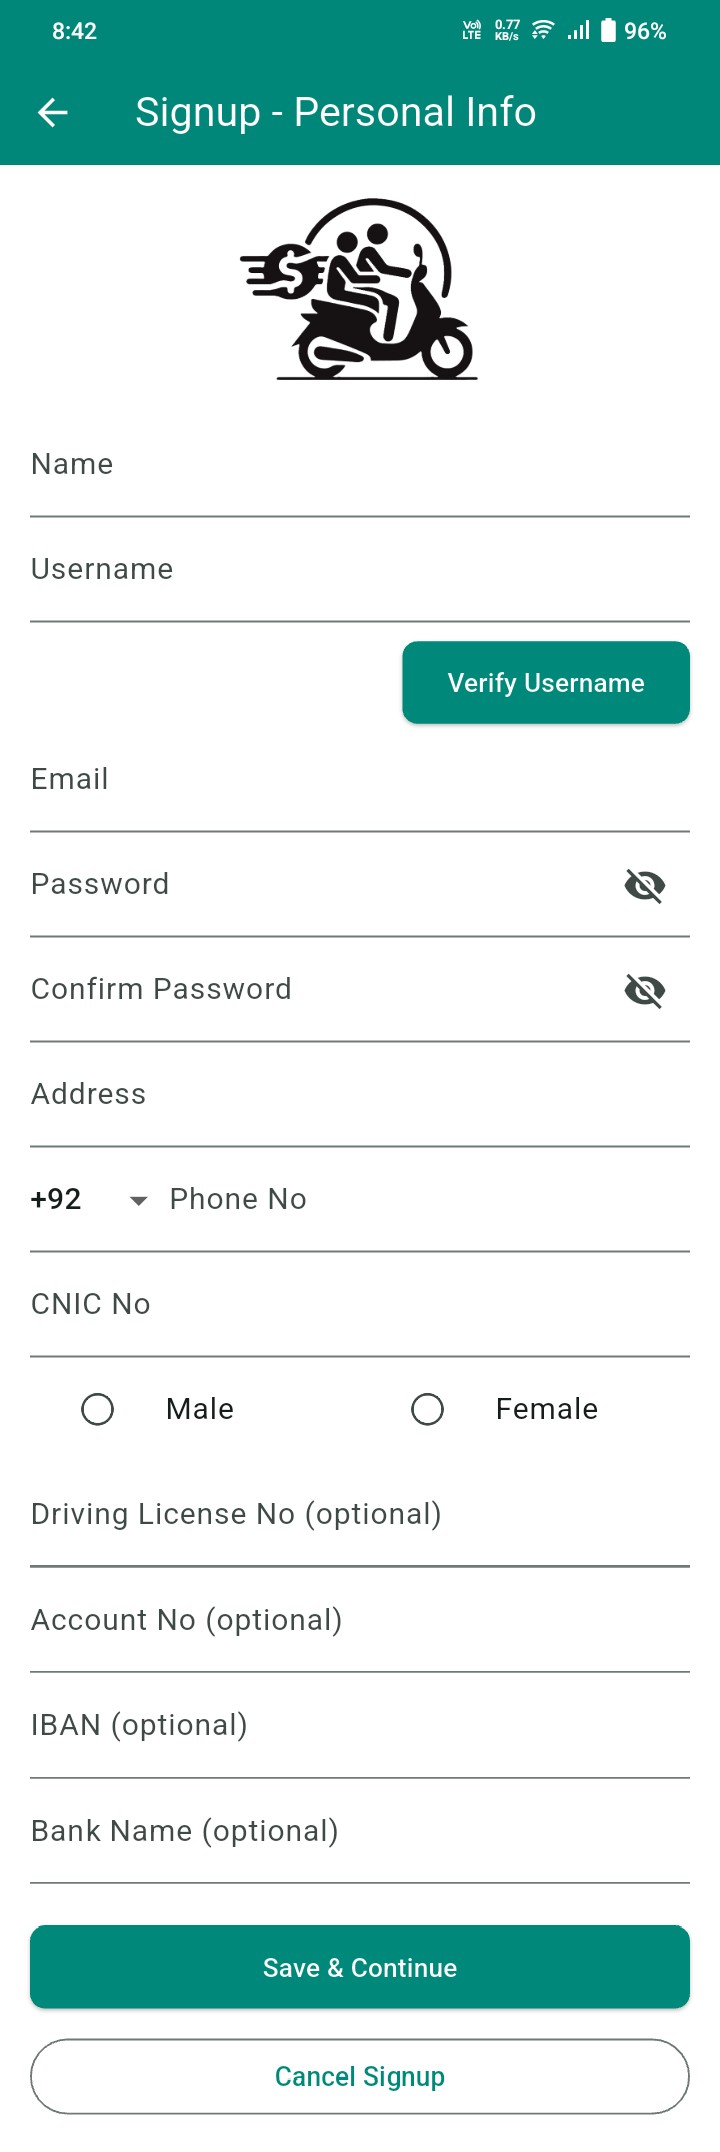
\includegraphics[width=\textwidth,keepaspectratio]{assets/app screenshot/signup_personal_info.jpeg}}
\end{minipage}\hfill
\begin{minipage}{0.23\textwidth}
\centering
\fbox{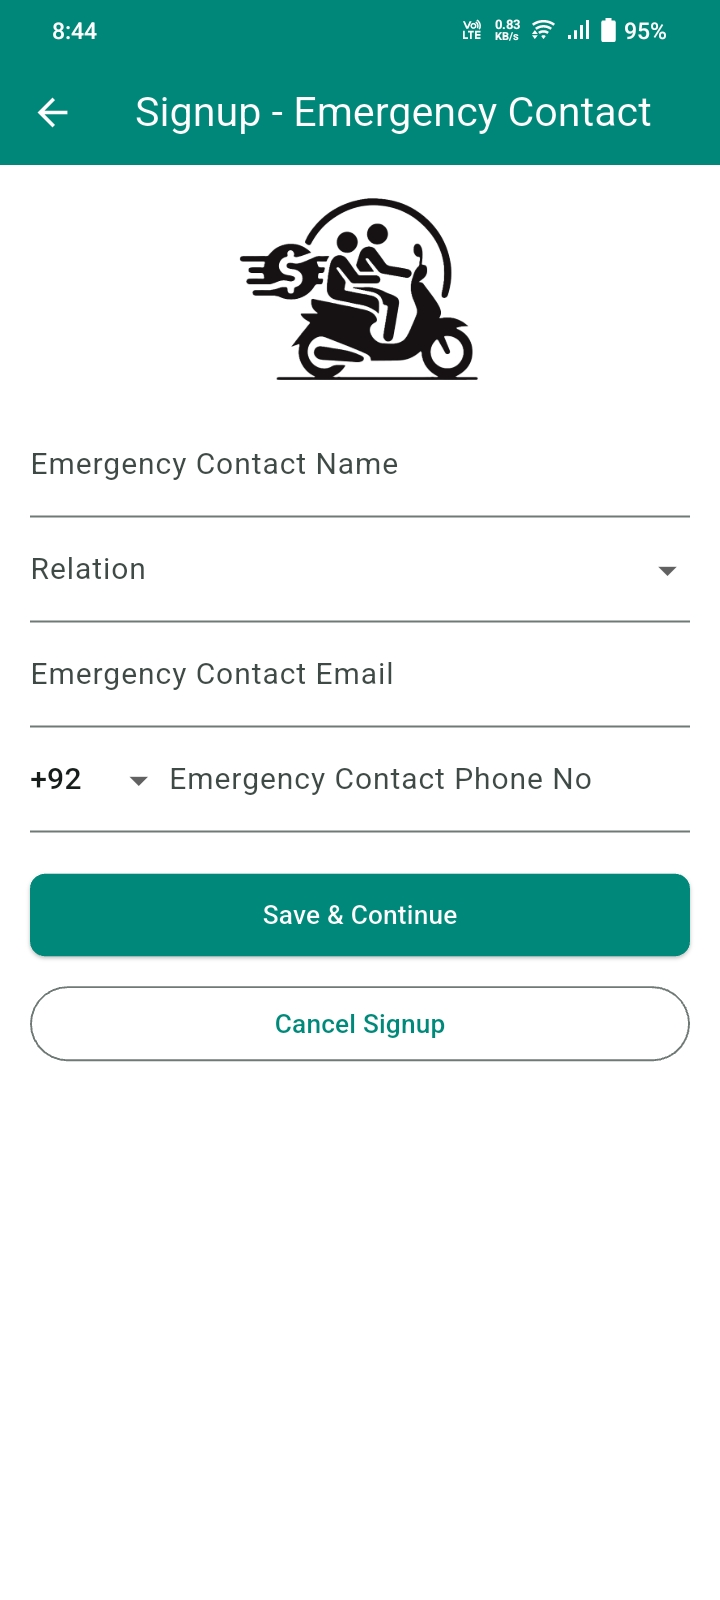
\includegraphics[width=\textwidth,keepaspectratio]{assets/app screenshot/signup_emergency_contact.jpeg}}
\end{minipage}\hfill
\begin{minipage}{0.23\textwidth}
\centering
\fbox{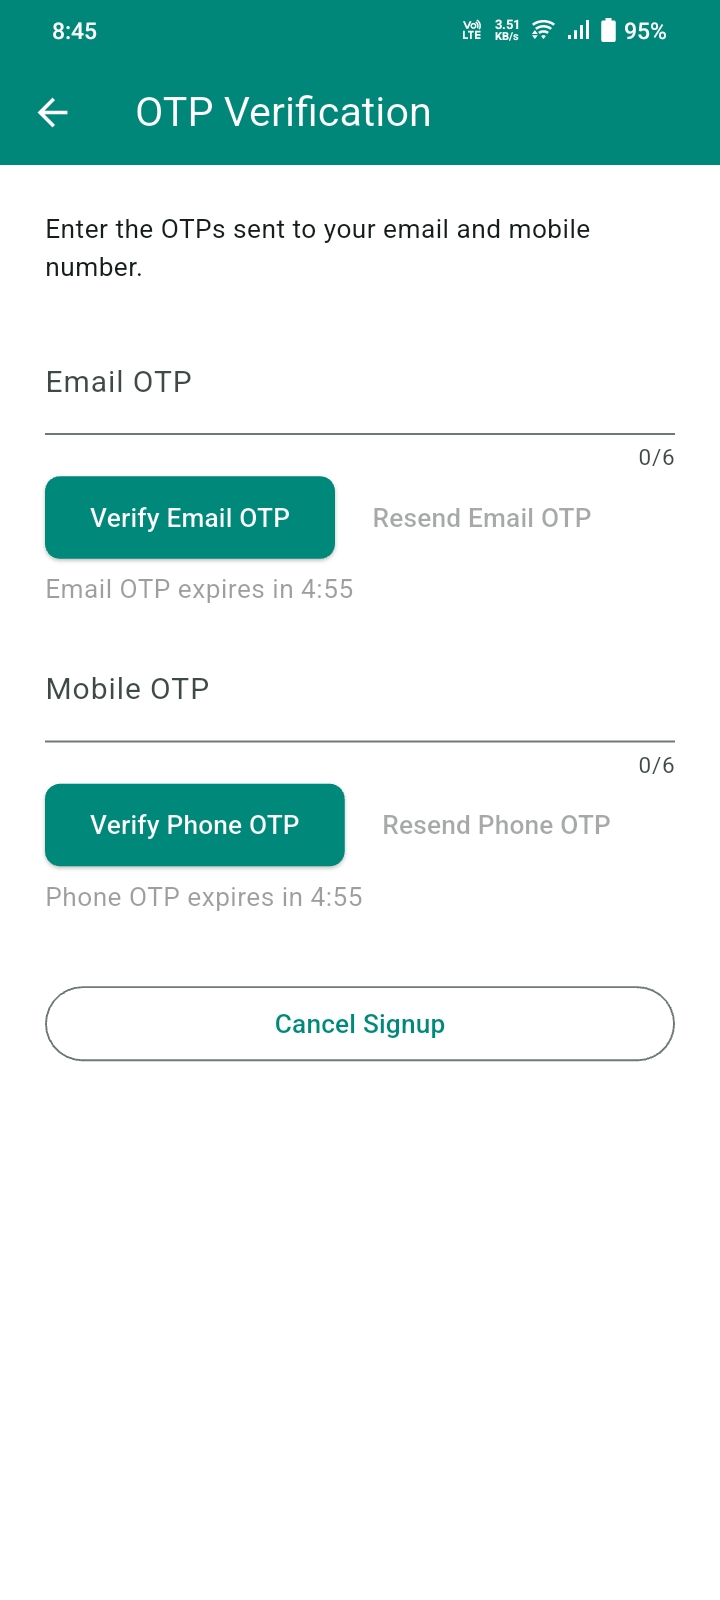
\includegraphics[width=\textwidth,keepaspectratio]{assets/app screenshot/signup_otp_verification.jpeg}}
\end{minipage}\hfill
\begin{minipage}{0.23\textwidth}
\centering
\fbox{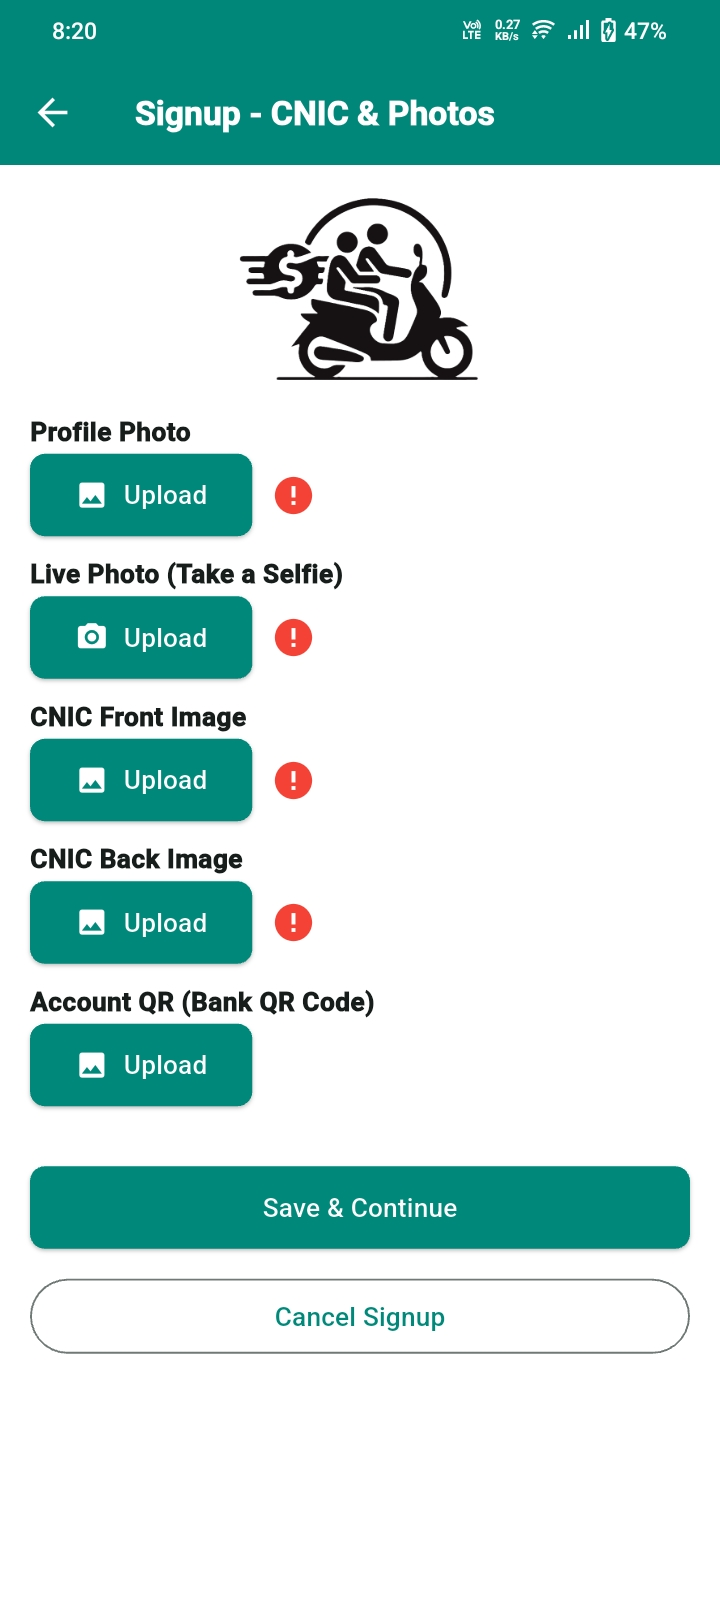
\includegraphics[width=\textwidth,keepaspectratio]{assets/app screenshot/signup_images uploading.jpg}}
\end{minipage}
\caption{User Signup Flow}
\end{figure}

\textbf{Functional Flow:} Enter personal and emergency contact details, upload required images and then complete OTP verification. If the OTP is validated successfully, then the user profile is created and the app moves on to the login/home flow based on the account status.

\textbf{Backend Integration:} Signup endpoints to register users and OTP verification to verify them, user profile data is stored in a backend database.

\textbf{Validation/Security:} Validator for required fields (client side), OTP expiry and retries implemented, validation for uploaded images implemented before submission.

\subsubsection{Screen 4: Login Screen}

\textbf{Function:} Where current users come from to use the platform.

\textbf{Components:}
\begin{itemize}
    \item Textboxes for text and password input.
    \item Remember Me checkbox.
    \item Type ``Login'' button and navigation to registration and forgot password flows.
\end{itemize}

\begin{figure}[H]
\centering
\fbox{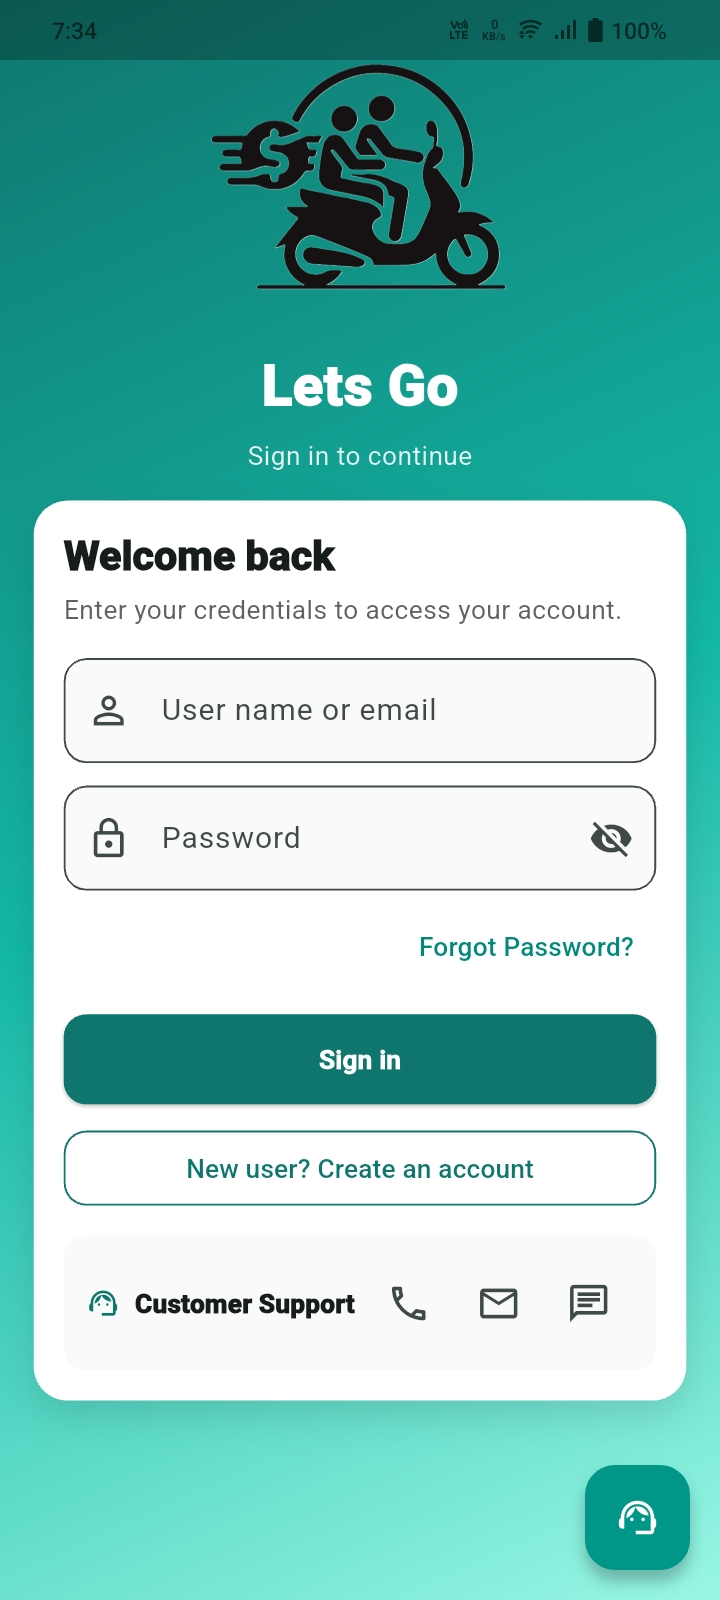
\includegraphics[width=0.45\textwidth,keepaspectratio,height=0.8\textheight]{assets/app screenshot/login_screen.jpeg}}
\caption{Login Screen}
\end{figure}

\textbf{Functional Flow:} The user enters the login information and clicks on the login form. A session is created and the user is taken to Home / Dashboard page if authentication is successful.

\textbf{Backend Integration:} The screen requests authentication credentials from the security end point to verify them and then requests the user profile payload to be used for navigation.

\textbf{Validation/Security:} Fields are blanked, error messages are provided if the credentials are invalid, and authentication calls are passed with session-based authorization.

\subsubsection{Screen 5: Account Status (Banned/Rejected)}

A screen displaying Account Status (Banned/Rejected).A screen that shows if the account is banned or rejected.

\textbf{Instructions:} If access is denied by Admin review, this will let the user know.

\textbf{Components:}
\begin{itemize}
    \item Status illustration and clear warning message.
    \item Contact Support option for appealing the decision.
\end{itemize}

\begin{figure}[H]
\centering
\begin{minipage}{0.30\textwidth}
\centering
\fbox{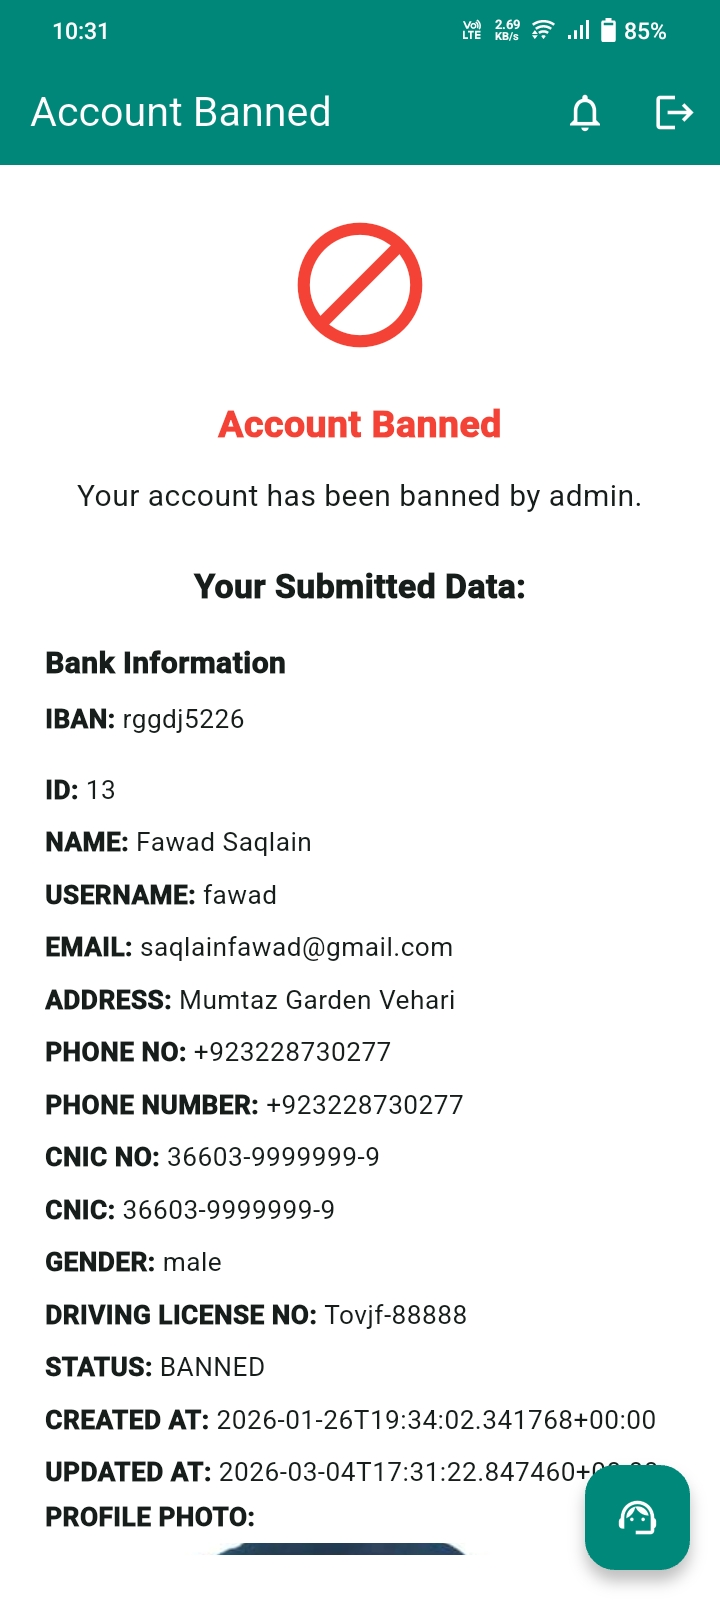
\includegraphics[width=\textwidth,keepaspectratio]{assets/app screenshot/account_banned.jpeg}}
\end{minipage}\hfill
\begin{minipage}{0.30\textwidth}
\centering
\fbox{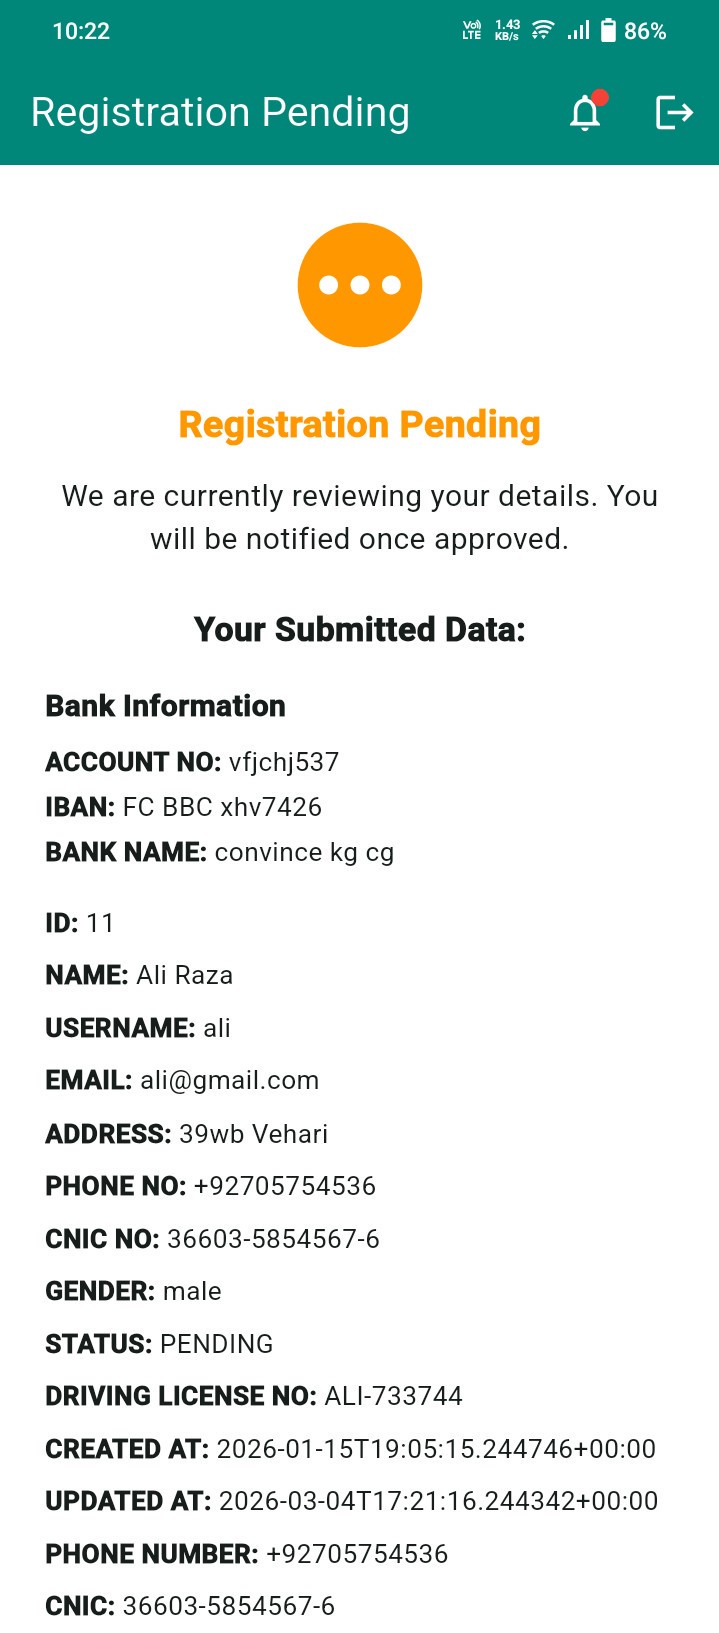
\includegraphics[width=\textwidth,keepaspectratio]{assets/app screenshot/account_pending.jpeg}}
\end{minipage}\hfill
\begin{minipage}{0.30\textwidth}
\centering
\fbox{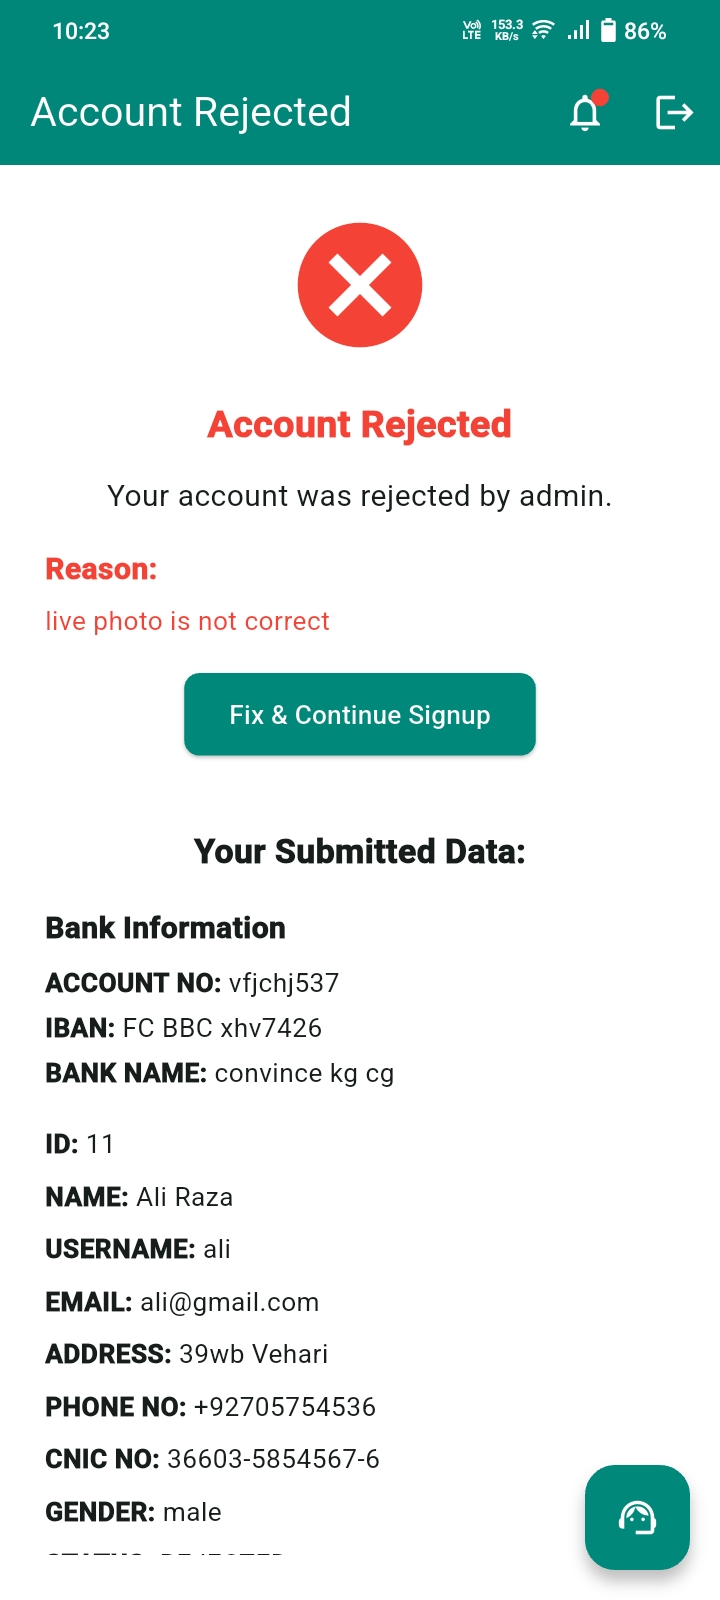
\includegraphics[width=\textwidth,keepaspectratio]{assets/app screenshot/account_rejected.jpeg}}
\end{minipage}
\caption{Account Status (Banned/Rejected)}
\end{figure}

\textbf{Login/signup and account status check:} This is a functional flow where after login/signup, the app validates the account status. When the account is pending, banned or rejected, the user is presented with a clear status screen with instructions and a support link.

\textbf{Backend Integration:} Status is taken from the user profile response and/or a status check endpoint.

\textbf{Server-side account gating:} Access to gated flows is denied if the user is not approved.

\subsubsection{Create Ride: Simplified Posting Flow}

\textbf{Purpose:} A driver ride posting simplified process from route selection to ride confirmation.

\begin{figure}[H]
\centering
\begin{minipage}{0.30\textwidth}
\centering
\fbox{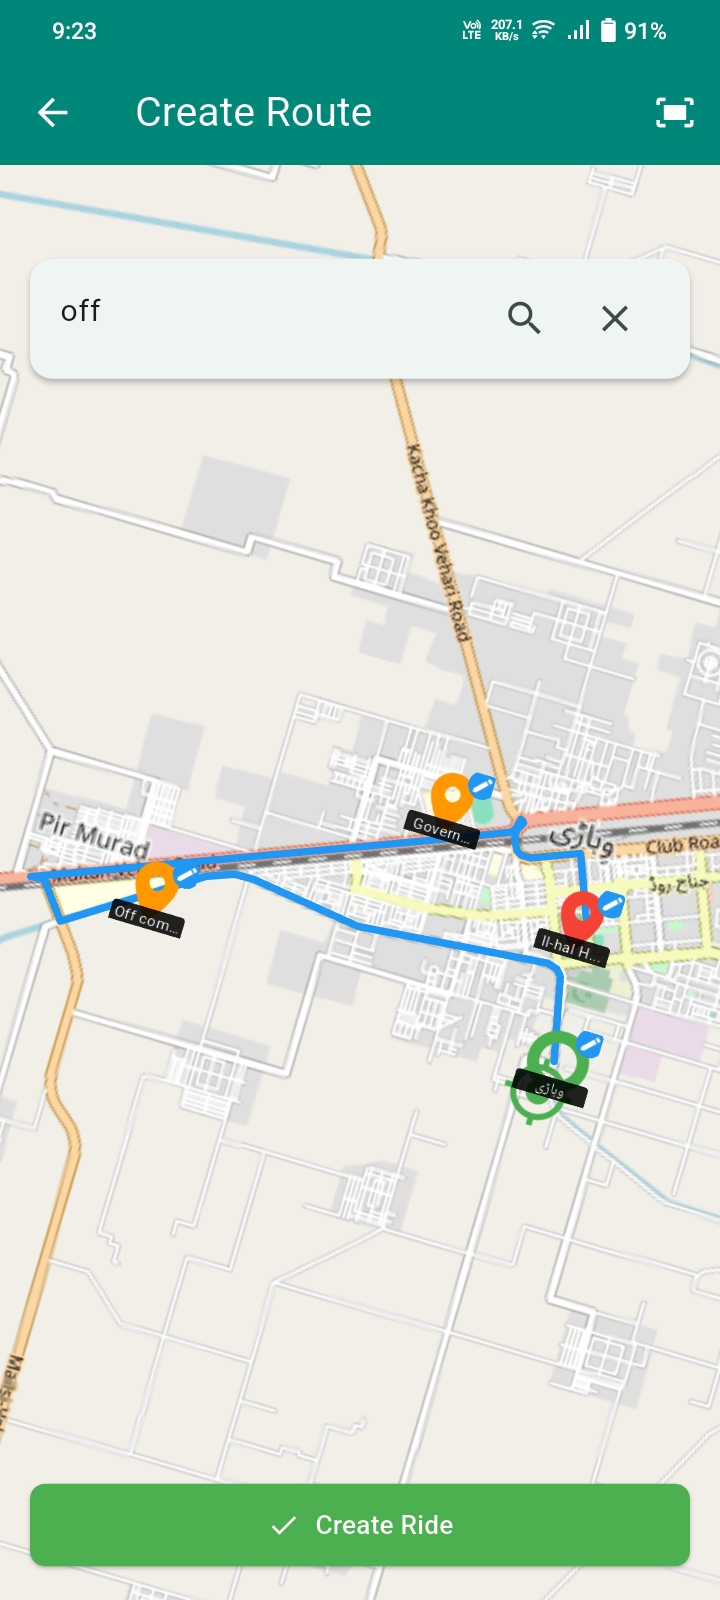
\includegraphics[width=\textwidth,keepaspectratio]{assets/app screenshot/create_route_map_view.jpeg}}
\end{minipage}\hfill
\begin{minipage}{0.30\textwidth}
\centering
\fbox{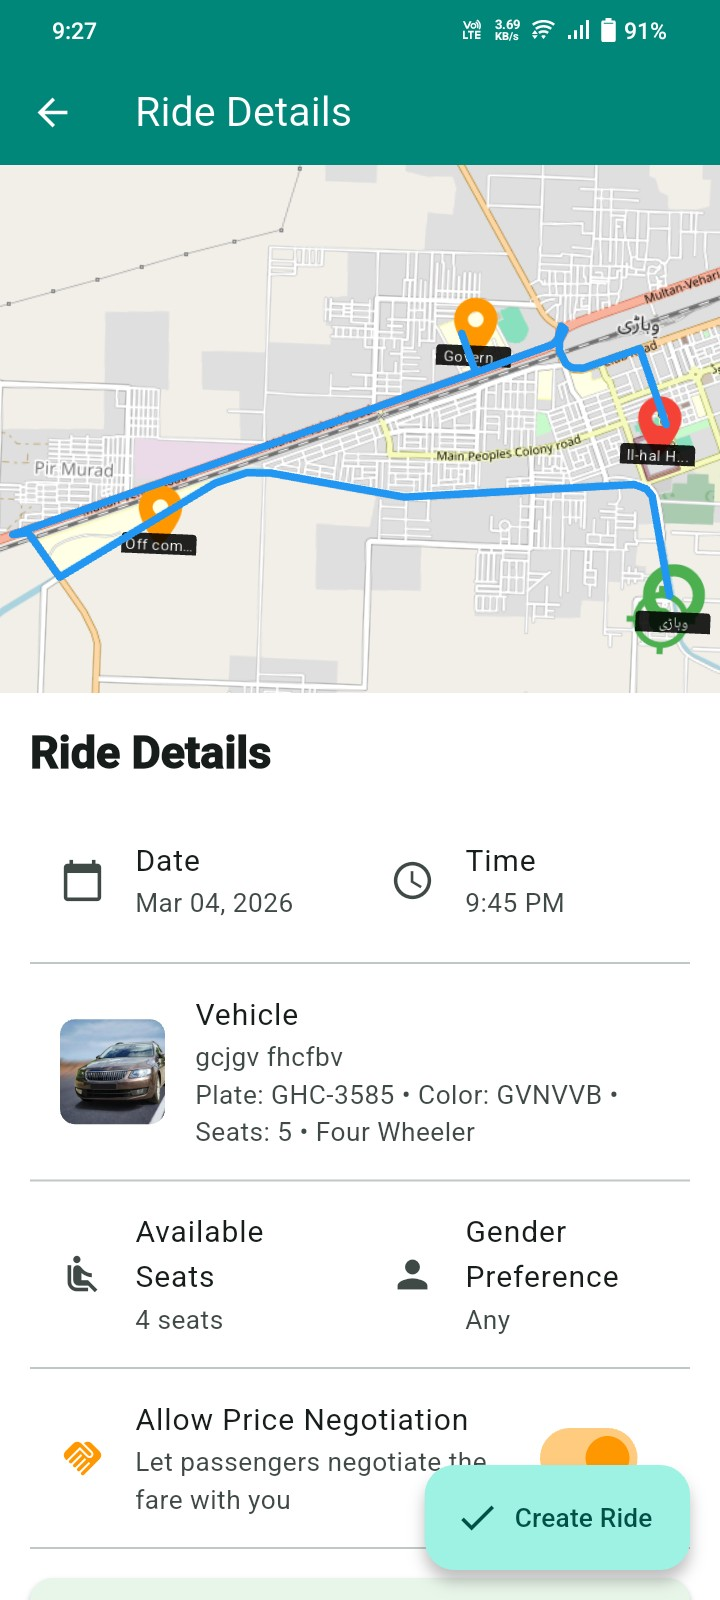
\includegraphics[width=\textwidth,keepaspectratio]{assets/app screenshot/create_ride_summary.jpeg}}
\end{minipage}\hfill
\begin{minipage}{0.30\textwidth}
\centering
\fbox{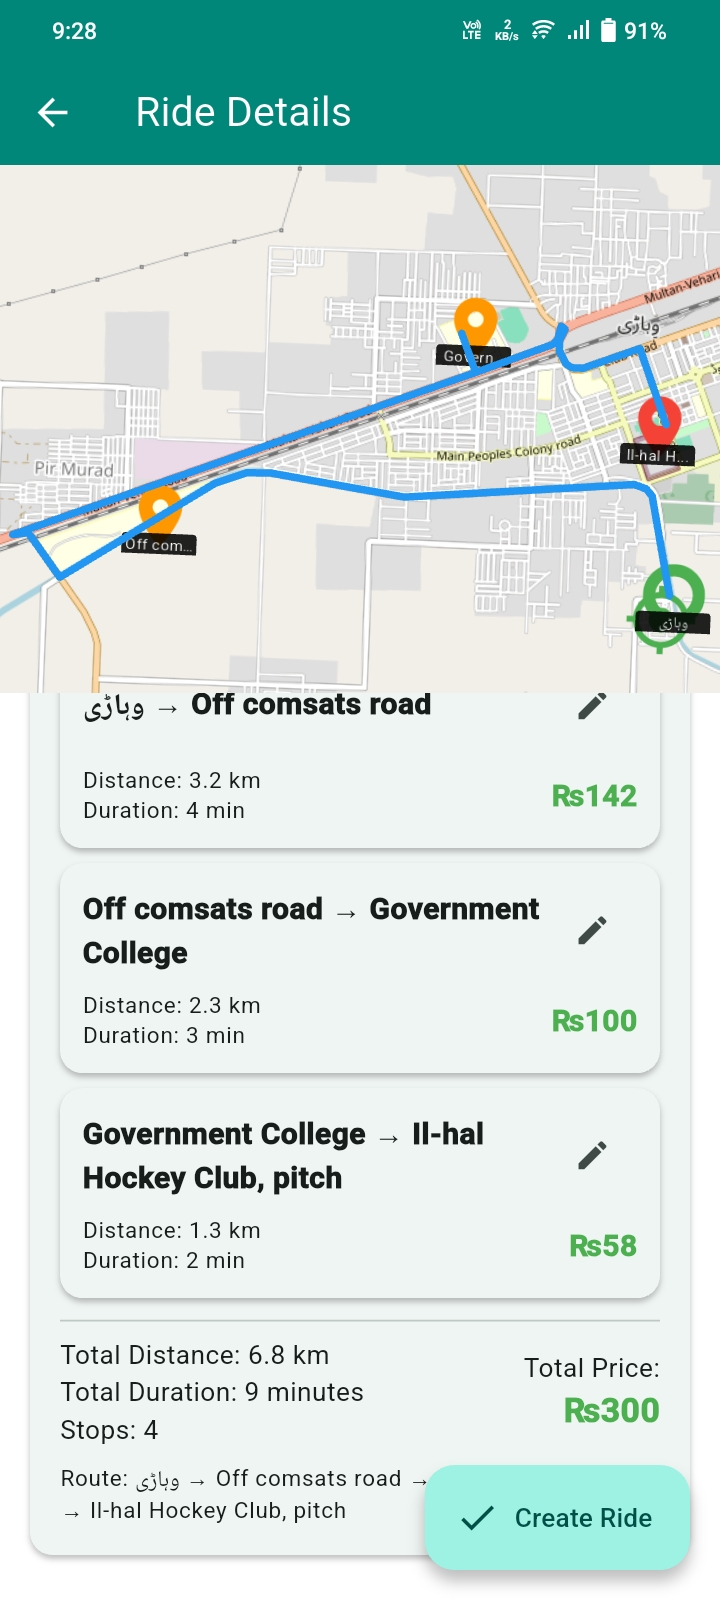
\includegraphics[width=\textwidth,keepaspectratio]{assets/app screenshot/create_ride_final_details.jpeg}}
\end{minipage}
\caption{Create Ride Posting Flow (Map View, Summary, and Final Details)}
\end{figure}

\textbf{Functional Flow:} Driver enters a route on the map, looks at a ridesummary and clears the final ride data and publishes the ride. Once the ride is submitted, it will appear in the passenger search results.

\textbf{Backend integration:} Flow calls ride creation endpoints and stores route geometries, stops, seats, and fare settings in the backend.

\textbf{Validation/Security:} Input constraints (seats, time, fare) are checked for validation and only validly authenticated drivers with valid profiles can post rides.

\subsubsection{Screen 14-16: Find Ride (Browse, Pickup/Drop, and Filters)}

\textbf{Goal:} User wants to see the available rides, choose which one to pickup/drop and filter the results.

\textbf{Components:}
\begin{itemize}
    \item Home and Work location search boxes.
    \item Visual location markers.
    \item Pickup/drop selection and ride filtering.
\end{itemize}

\begin{figure}[H]
\centering
\begin{minipage}{0.30\textwidth}
\centering
\fbox{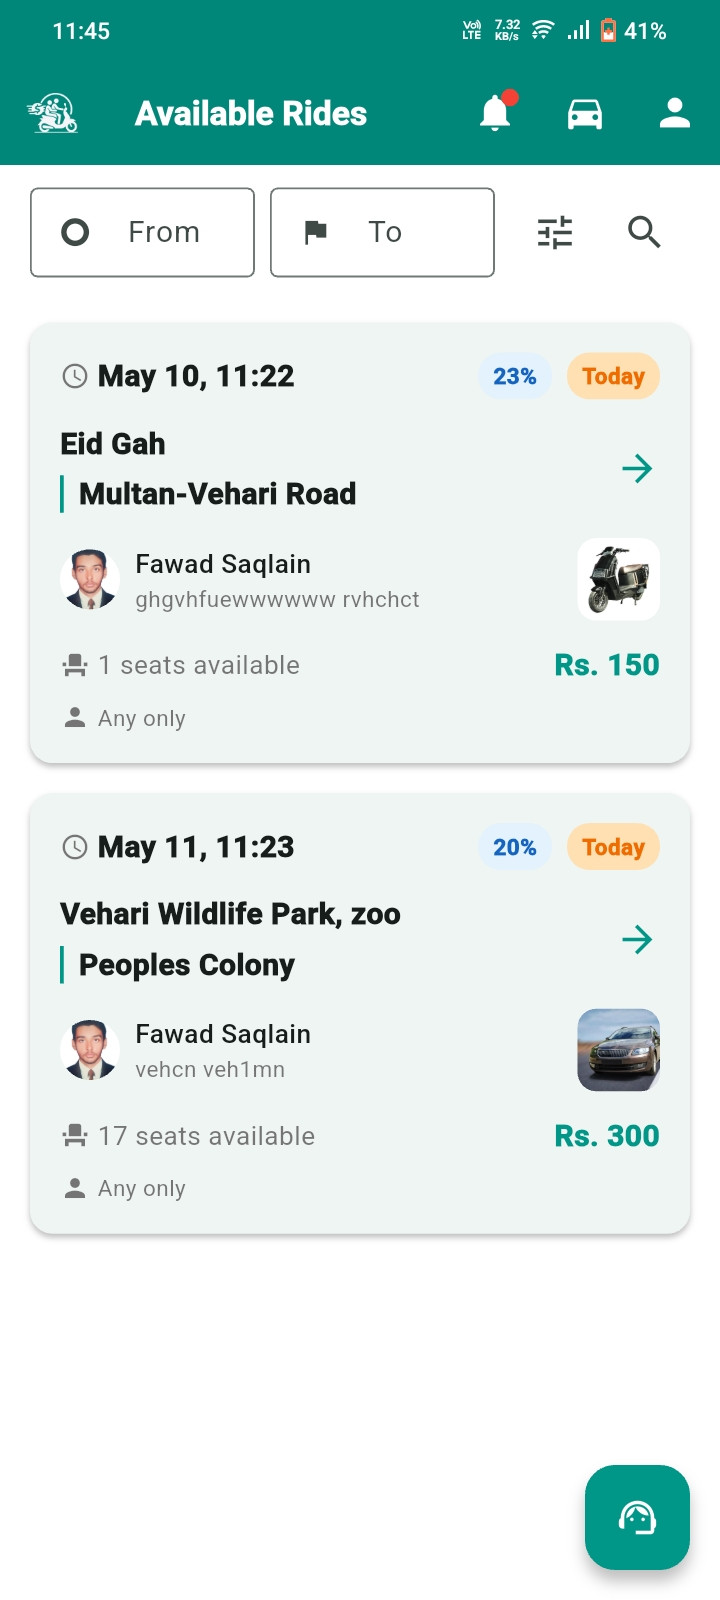
\includegraphics[width=\textwidth,keepaspectratio]{assets/app screenshot/find_ride_available_rides.jpeg}}
\end{minipage}\hfill
\begin{minipage}{0.30\textwidth}
\centering
\fbox{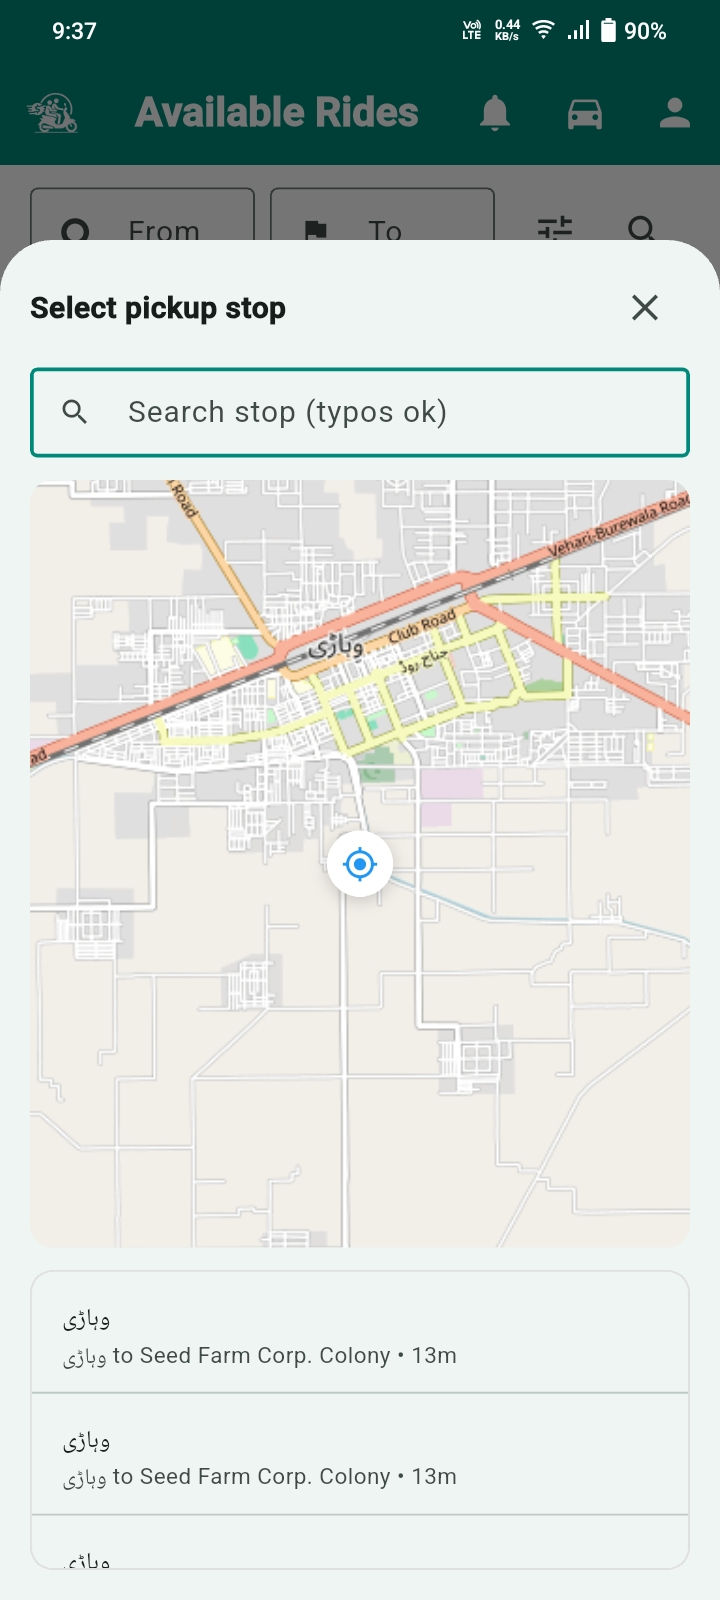
\includegraphics[width=\textwidth,keepaspectratio]{assets/app screenshot/find_ride_select_pickup.jpeg}}
\end{minipage}\hfill
\begin{minipage}{0.30\textwidth}
\centering
\fbox{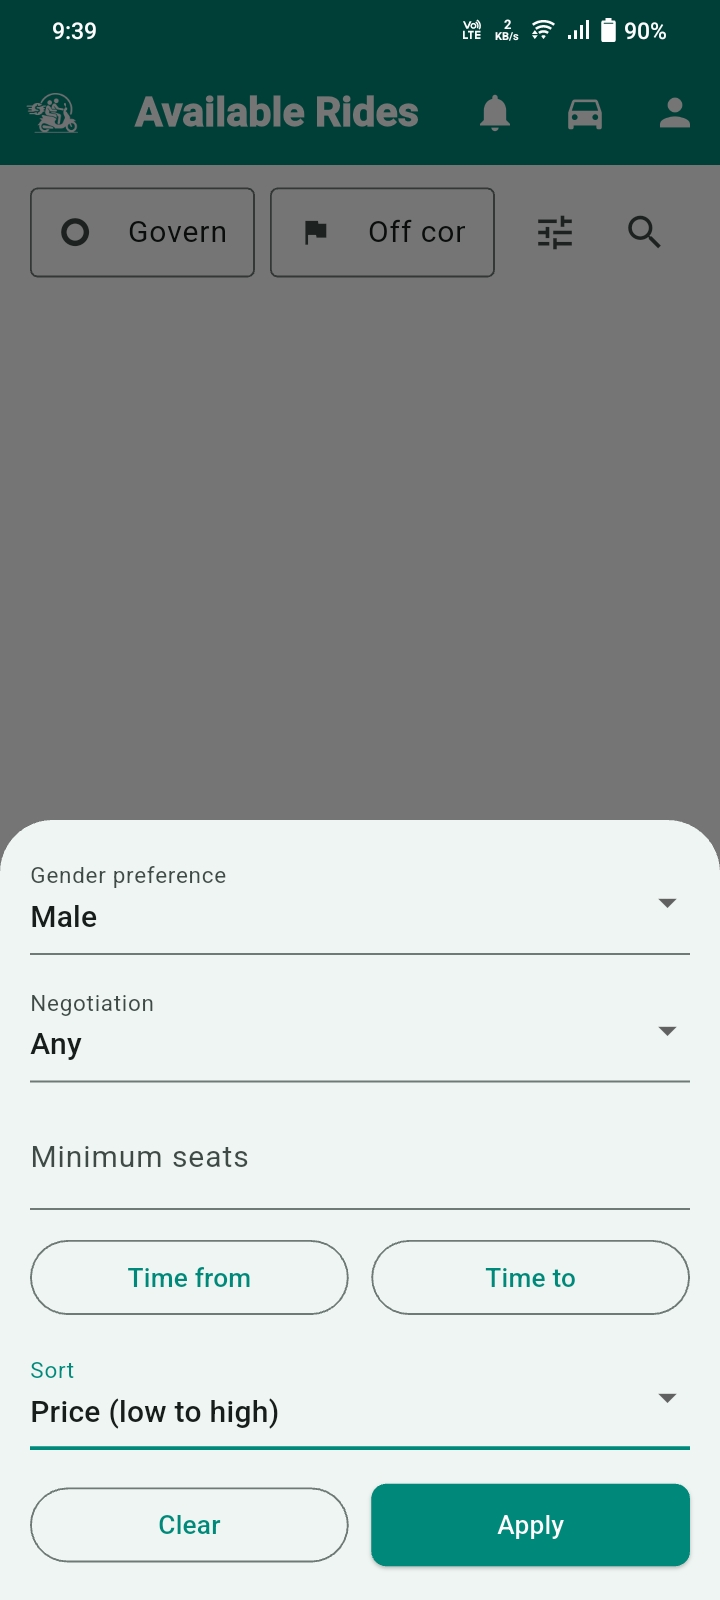
\includegraphics[width=\textwidth,keepaspectratio]{assets/app screenshot/find_ride_filters.jpeg}}
\end{minipage}
\caption{Find Ride Flow (Available Rides, Pickup/Drop, and Filters)}
\end{figure}

\textbf{Functional Flow:} The Functional Flow is pretty easy to use: Users review a list of rides, choose a pickup location, choose a drop location, and use a filter to narrow their choices. Clicking on ``Select a ride'' will switch to the Ride Details view.

\textbf{Backend Integration:} Search Endpoints: The list and filters are driven by trip search end points which include query parameters like route, time window and seat availability.

\textbf{Validation/Security:} Filters are sanitized and results are limited to the current user session and platform rules.

\subsubsection{Screen 17: Ride Details View}

The Ride Details View is the next screen.The next screen is the Ride Details View.

\textbf{Aim:} All ride parameters for passenger review detailed.

\textbf{Components:}
\begin{itemize}
    \item Driver profile, vehicle information and trip timeline.
\end{itemize}

\begin{figure}[H]
\centering
\begin{minipage}{0.45\textwidth}
\centering
\fbox{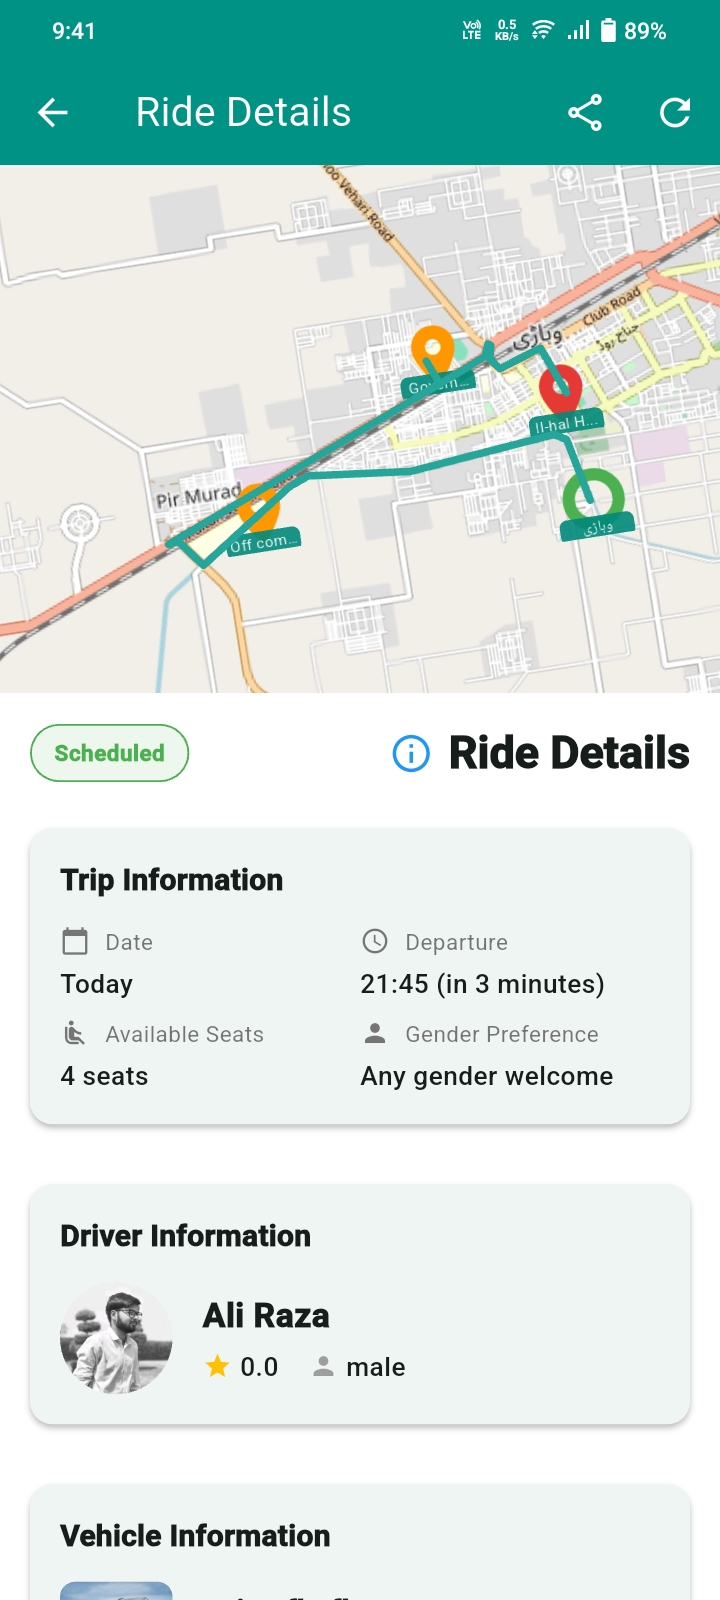
\includegraphics[width=\textwidth,keepaspectratio]{assets/app screenshot/ride_details part 1.jpeg}}
\end{minipage}\hfill
\begin{minipage}{0.45\textwidth}
\centering
\fbox{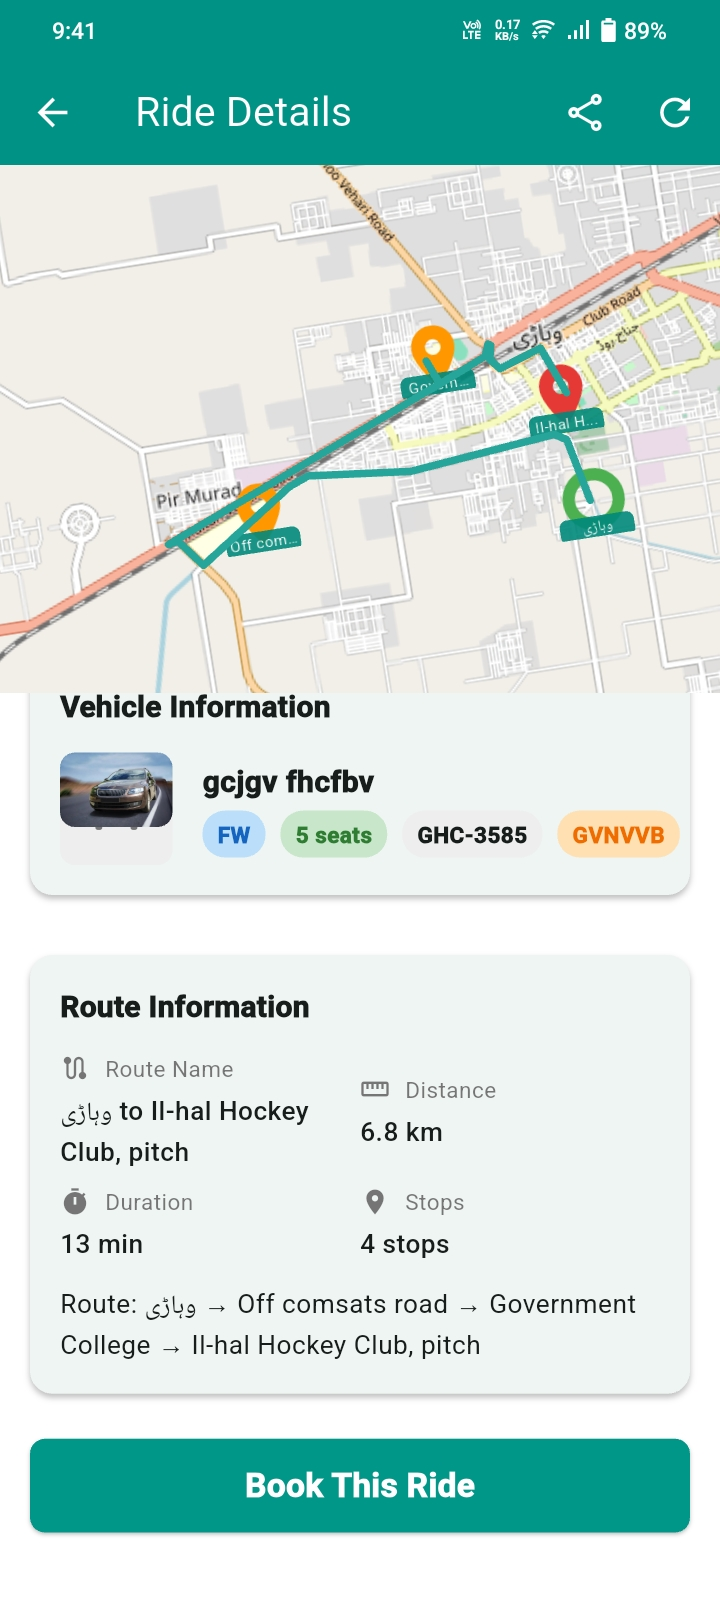
\includegraphics[width=\textwidth,keepaspectratio]{assets/app screenshot/ride_details part 2.jpeg}}
\end{minipage}
\caption{Ride Details View}
\end{figure}

\textbf{Functional Flow:} The passenger reads the driver and ride information (route and time) and then goes to the booking/request screen. This screen is used to confirm a booking prior to making a booking.

\textbf{Backend Integration:} Rides are retrieved from the backend using the trip identifier and will contain data like driver profile and stops.

\textbf{Validation/Security:} The UI hides actions if the ride is unavailable and blocks booking without valid session context.

\subsubsection{Screen 18: Request Ride (Booking Form)}

\textbf{Use case:} Enables passengers to view the route overview and to submit a ride request with seat selection, optional price negotiation and special notes.

\textbf{Components:}
\begin{itemize}
    \item An overview map and trip report (date, time, length of trip, cost of trip).
    \item Negotiation input, seat selection, and gender selection in pick-up/drop-off.
\end{itemize}

\begin{figure}[H]
\centering
\begin{minipage}{0.40\textwidth}
\centering
\fbox{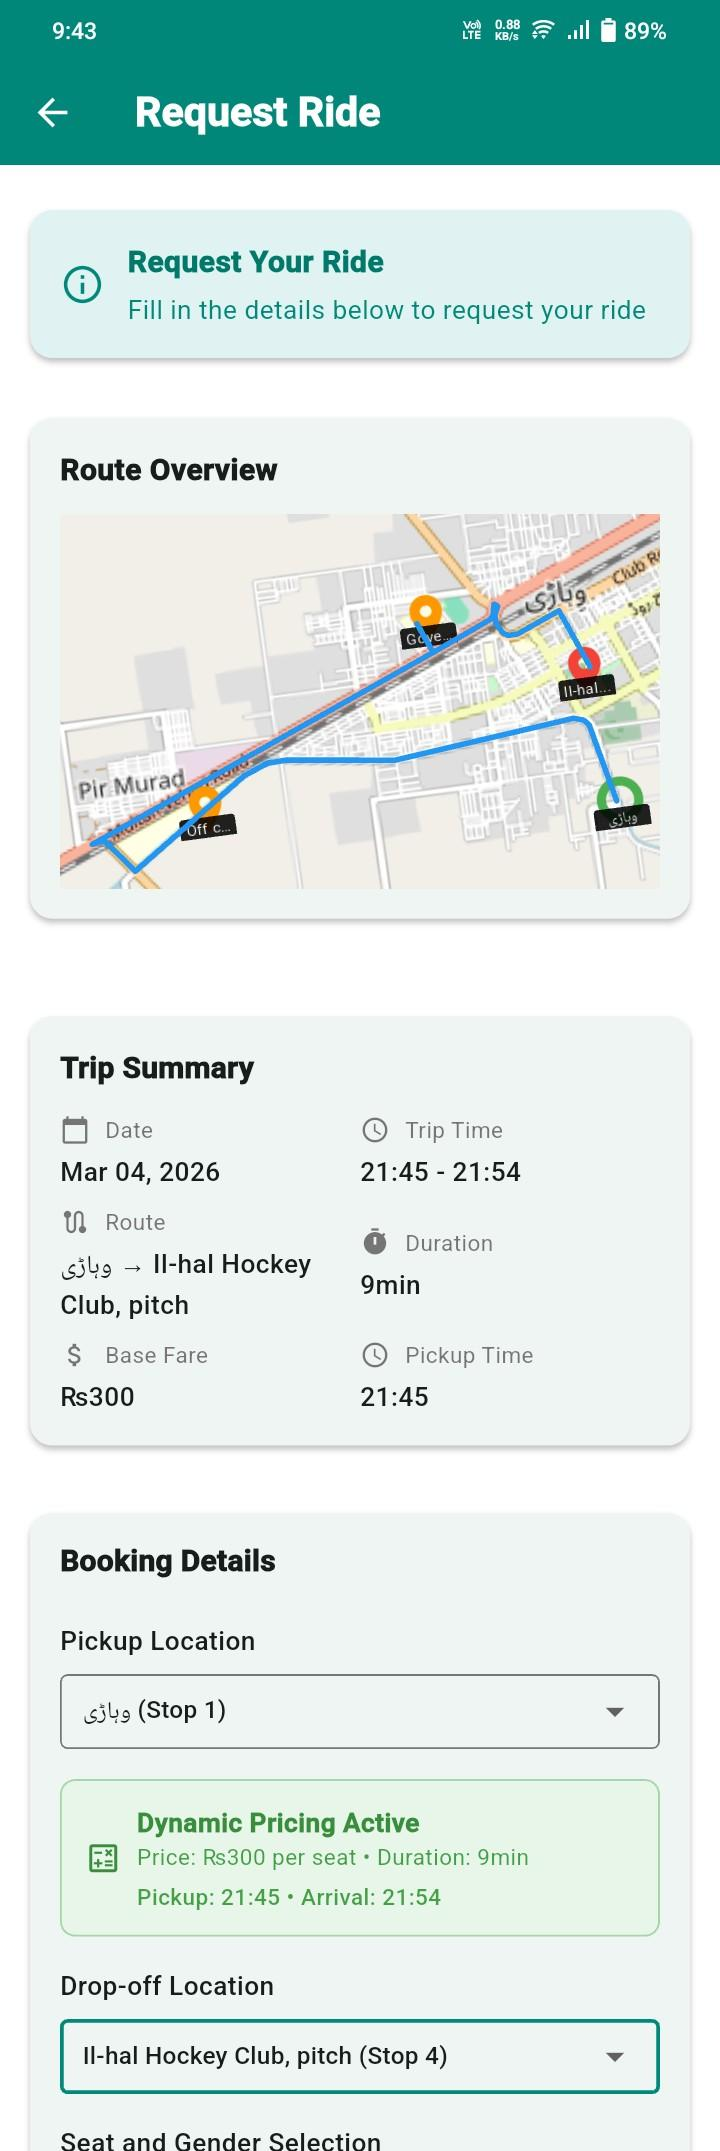
\includegraphics[width=\textwidth,height=0.72\textheight,keepaspectratio]{assets/app screenshot/ride_request_part1.jpeg}}
\end{minipage}\hfill
\begin{minipage}{0.40\textwidth}
\centering
\fbox{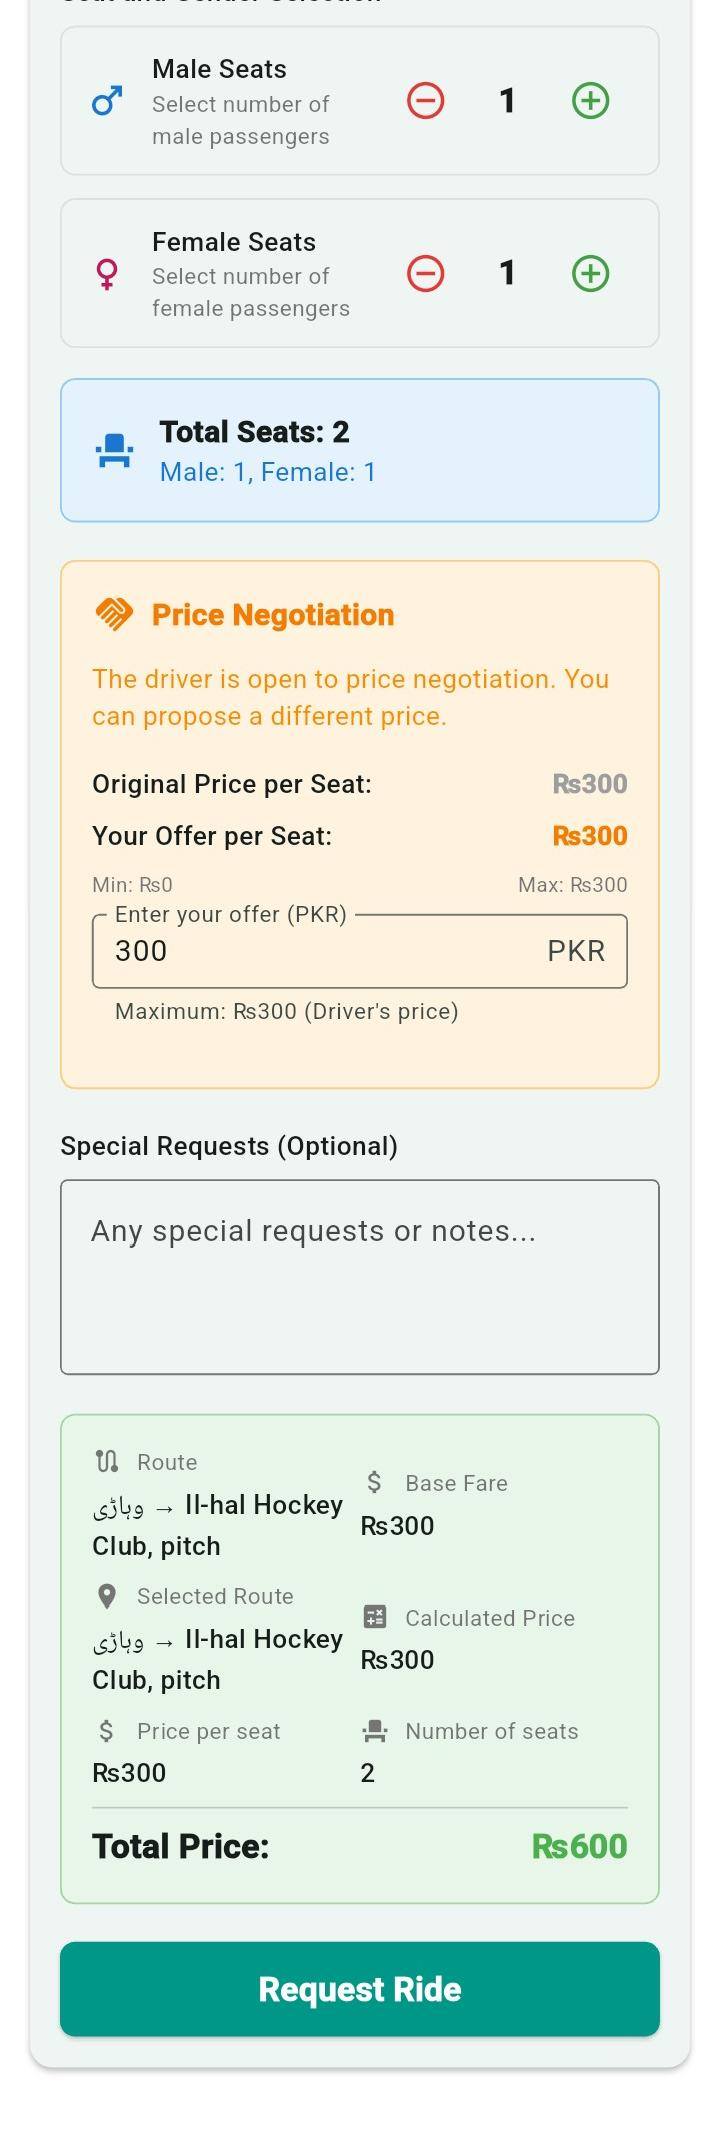
\includegraphics[width=\textwidth,height=0.72\textheight,keepaspectratio]{assets/app screenshot/ride_request_part2.jpeg}}
\end{minipage}
\caption{Request Ride (Booking Form)}
\end{figure}

\textbf{Functional Flow:} Passenger chooses pickup/drop stops and seats, optionally offers counter fare, submits request. The request will then be in a pending/negotiation state until the driver responds.

\textbf{Backend Integration:} Sends a booking request payload which is associated with the trip and passenger profile and sends notifications for driver review.

\textbf{Validation/Security:} If more people than seats are available, the reservation is not processed and if a wrong stop is selected, it is rejected.

\subsubsection{Screen 19: Booked Ride Details}

\textbf{Aim:} Choosing seats and confirming booking conditions.

\textbf{Components:}
\begin{itemize}
    \item Number of seats available, and certain seating choices.
\end{itemize}

\begin{figure}[H]
\centering
\begin{minipage}{0.45\textwidth}
\centering
\fbox{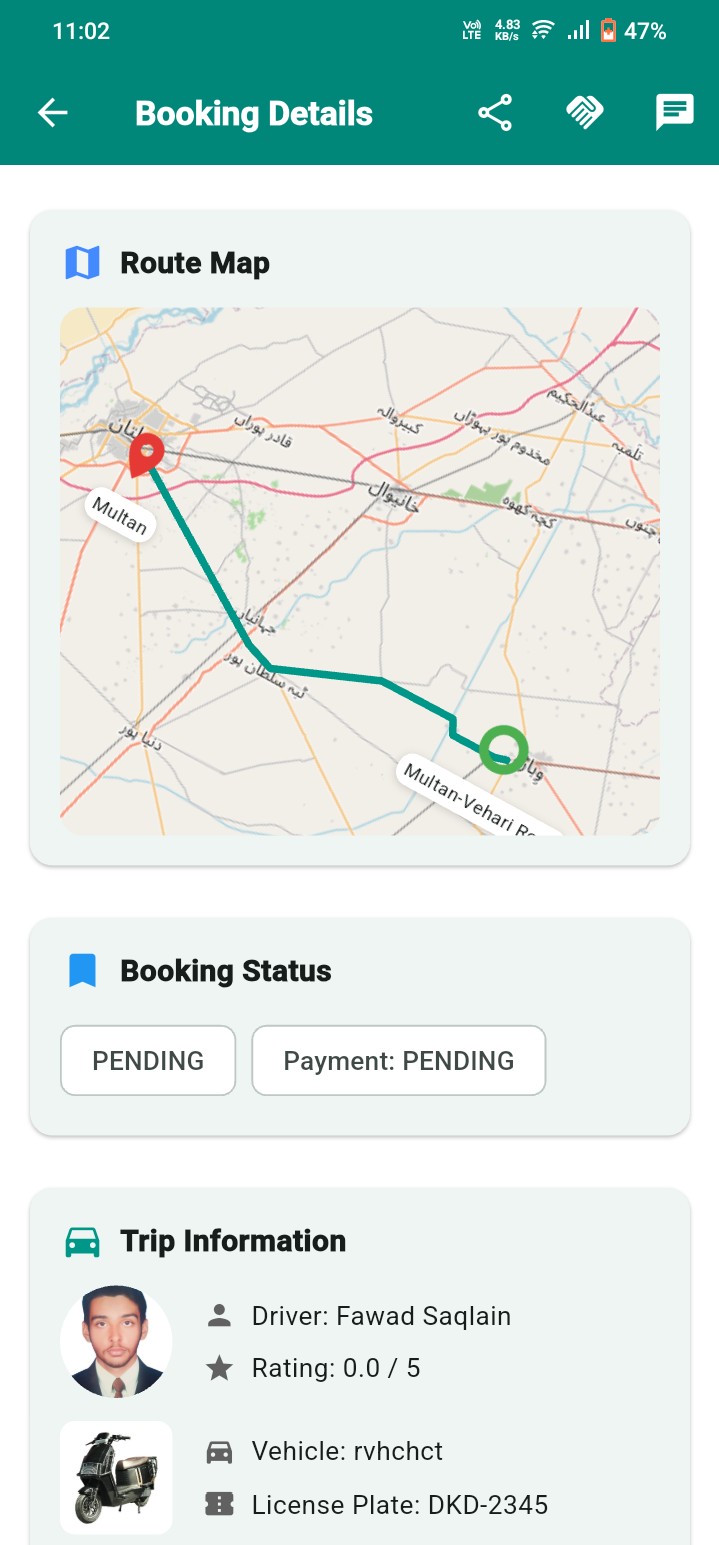
\includegraphics[width=\textwidth,height=0.42\textheight,keepaspectratio]{assets/app screenshot/passenger_booking_details_pending part 1.jpeg}}
\end{minipage}\hfill
\begin{minipage}{0.45\textwidth}
\centering
\fbox{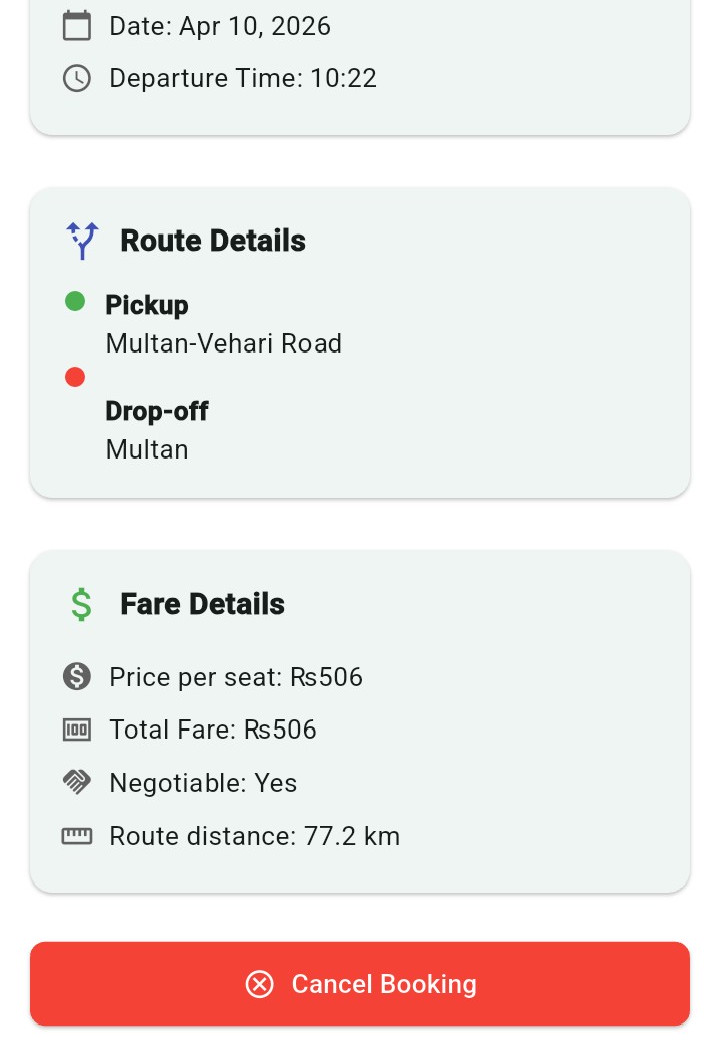
\includegraphics[width=\textwidth,keepaspectratio]{assets/app screenshot/passenger_booking_details_pending part 2.jpeg}}
\end{minipage}
\caption{Booked Ride Details}
\end{figure}

\textbf{Functional Flow:} After the booking is completed, the passenger sees the booking details and the seat allocation state. The screen is updated as the driver accepts, rejects or negotiates with the updates.

\textbf{Backend Integration:} loads booking information from the bookings endpoints and will periodically refresh for state changes.

\textbf{Validation/Security:} Only the owner of the booking is able to see the details and sensitive fields are limited by role.

\subsubsection{Screen 21: Negotiation Between Passenger and Driver}

This can be used when negotiating the price when booking, where both the driver and passenger can view and comment on the negotiation.

\textbf{Components:}
\begin{itemize}
    \item Information about negotiations and counter offers.
    \item Response controls and request status update.
\end{itemize}

\begin{figure}[H]
\centering
\begin{minipage}{0.30\textwidth}
\centering
\fbox{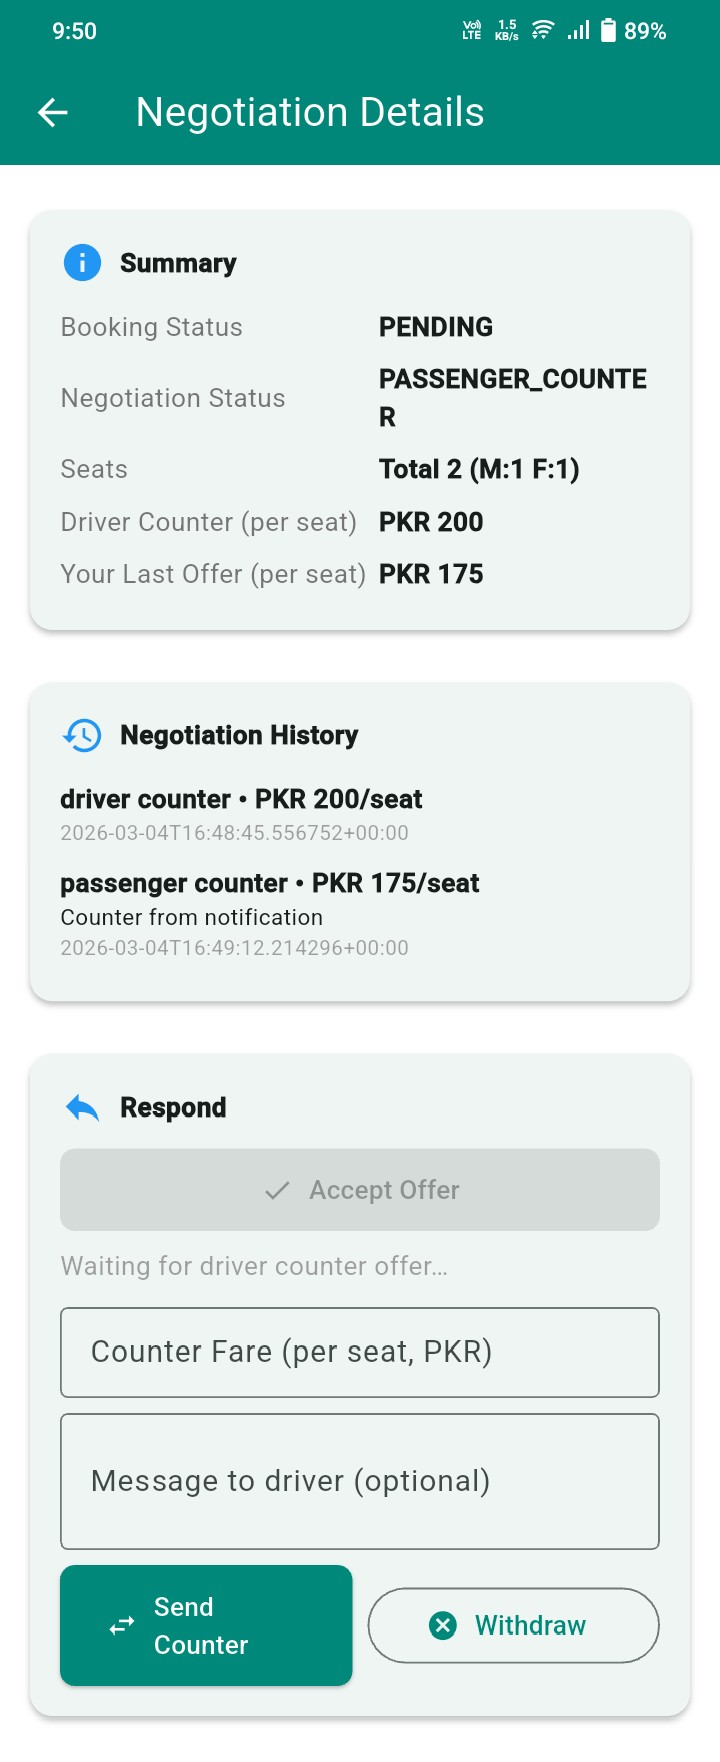
\includegraphics[width=\textwidth,keepaspectratio]{assets/app screenshot/passenger_negotiation_details.jpeg}}
\end{minipage}\hfill
\begin{minipage}{0.30\textwidth}
\centering
\fbox{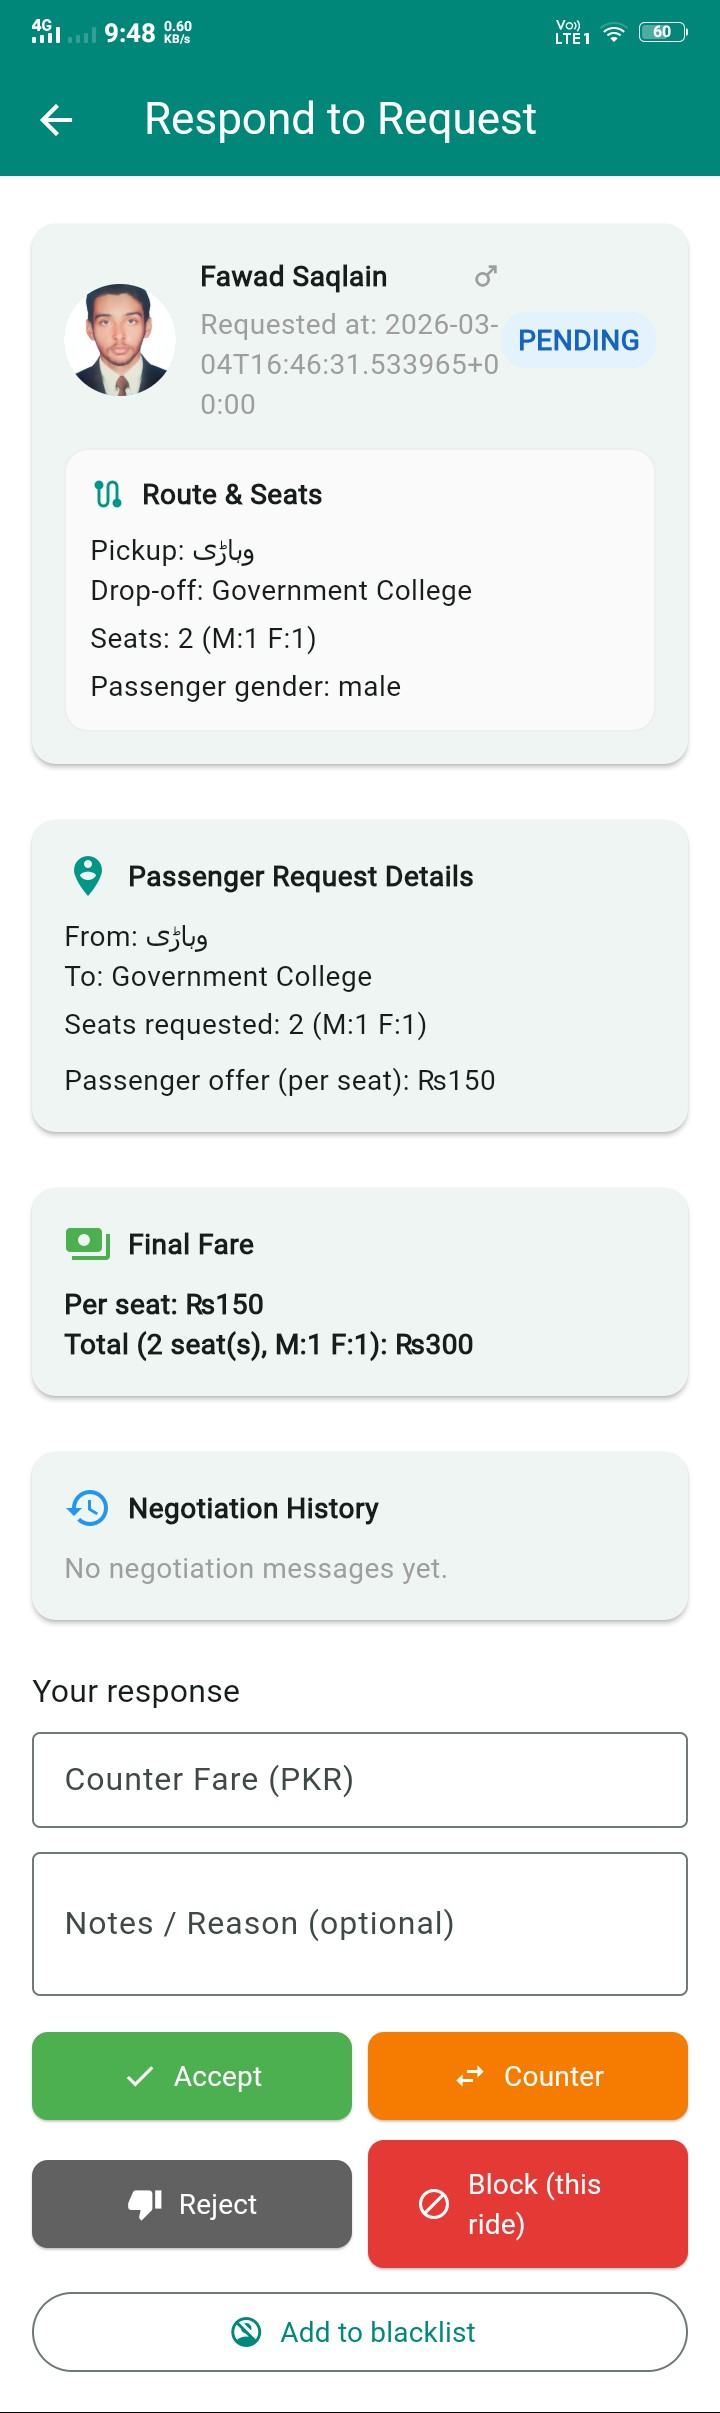
\includegraphics[width=\textwidth,keepaspectratio]{assets/app screenshot/driver_response_screen.jpeg}}
\end{minipage}\hfill
\begin{minipage}{0.30\textwidth}
\centering
\fbox{
\includegraphics[width=\textwidth,keepaspectratio]{assets/app screenshot/driver_ride_requests_pending.jpeg}}
\end{minipage}
\caption{Negotiation Between Passenger and Driver}
\end{figure}

When the passenger and driver offer and discuss fares, they do so until they arrive at a final fare, or the passenger backs out of the deal. The UI shows the most recent offer and the action permitted next.

\textbf{Backend Integration:} Update the booking state with negotiation history endpoints, and submit/accept/counter actions.

\textbf{Validation/Security:} Only valid users on the booking can negotiate, server rules are used to prevent invalid state transitions.

\subsubsection{Screen 22: Driver Ride Details (Pending)}

\textbf{Purpose:} Provides information about the ride request in detail for driver review prior to acceptance or rejection.

\textbf{Components:}
\begin{itemize}
    \item Passenger information, route overview and approval management.
\end{itemize}

\begin{figure}[H]
\centering
\begin{minipage}{0.45\textwidth}
\centering
\fbox{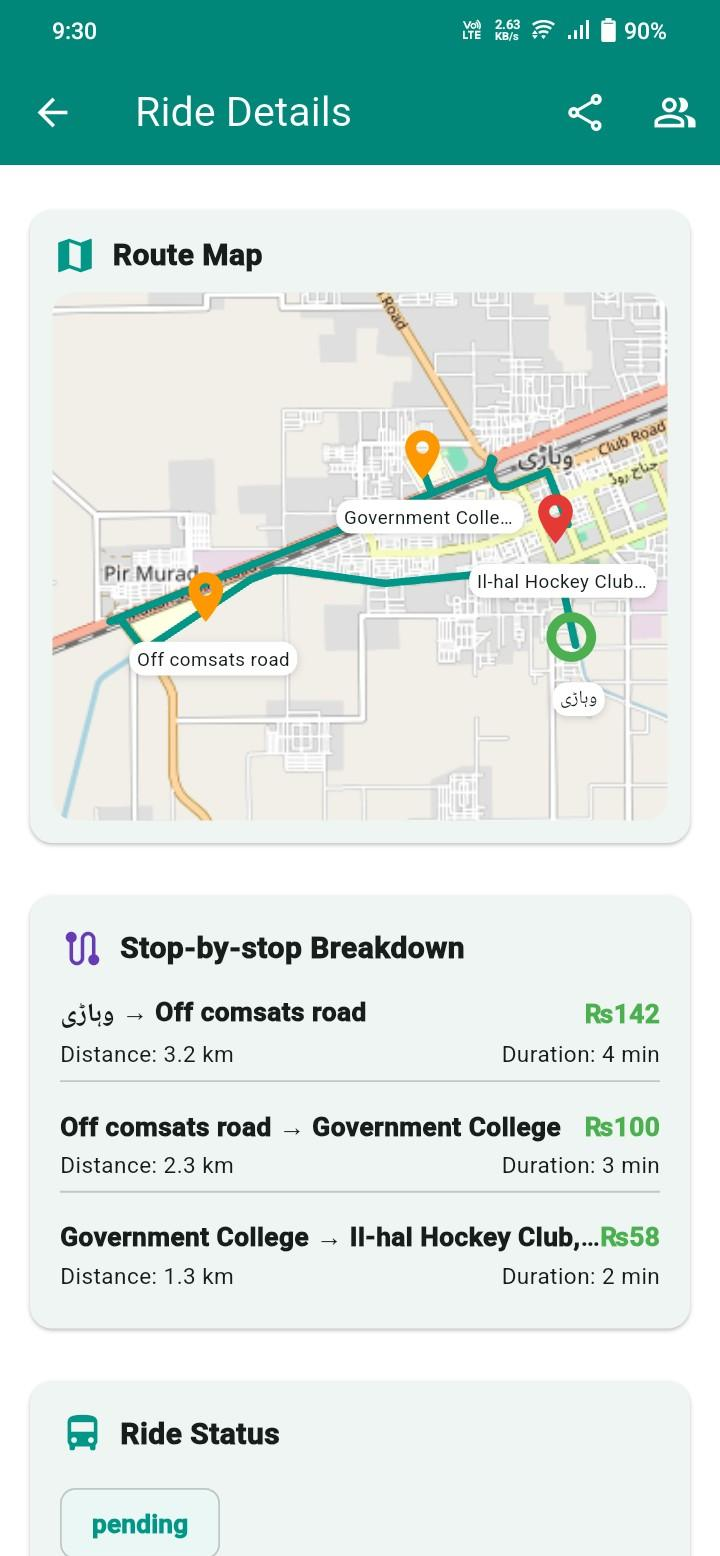
\includegraphics[width=\textwidth,height=0.52\textheight,keepaspectratio]{assets/app screenshot/driver_ride_details_pending_part1.jpeg}}
\end{minipage}\hfill
\begin{minipage}{0.45\textwidth}
\centering
\fbox{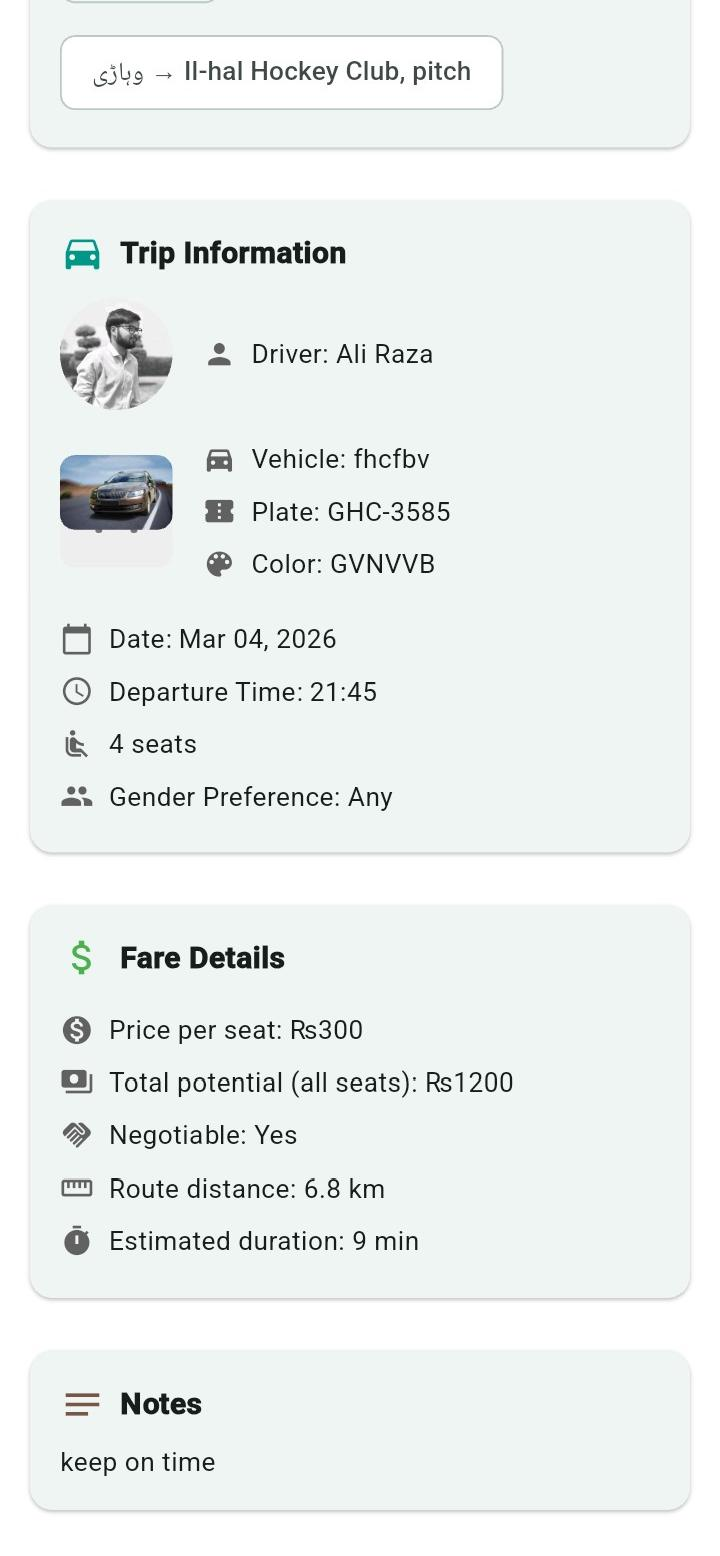
\includegraphics[width=\textwidth,height=0.52\textheight,keepaspectratio]{assets/app screenshot/driver_ride_details_pending_part2.jpeg}}
\end{minipage}
\caption{Driver Ride Details (Pending)}
\end{figure}

Functional Flow: Driver sees the work order and accepts/rejects or takes up negotiation. Passenger facing status updates instantly when driver actions are done.

\textbf{Backend Integration:} Driver actions are made to a booking decision Endpoint that updates booking status and sends notifications.

\textbf{Validation/Security:} only the trip owner can approve requests, backend checks prevent requests if there are not enough seats available.

\subsubsection{Screen 23: Negotiation Completed}

\textbf{Purpose:} Confirms that the negotiation is finalized and the booking request is accepted by both driver and passenger.

\textbf{Components:}
\begin{itemize}
    \item Acceptance confirmation and updated request status.
\end{itemize}

\begin{figure}[H]
\centering
\begin{minipage}{0.45\textwidth}
\centering
\fbox{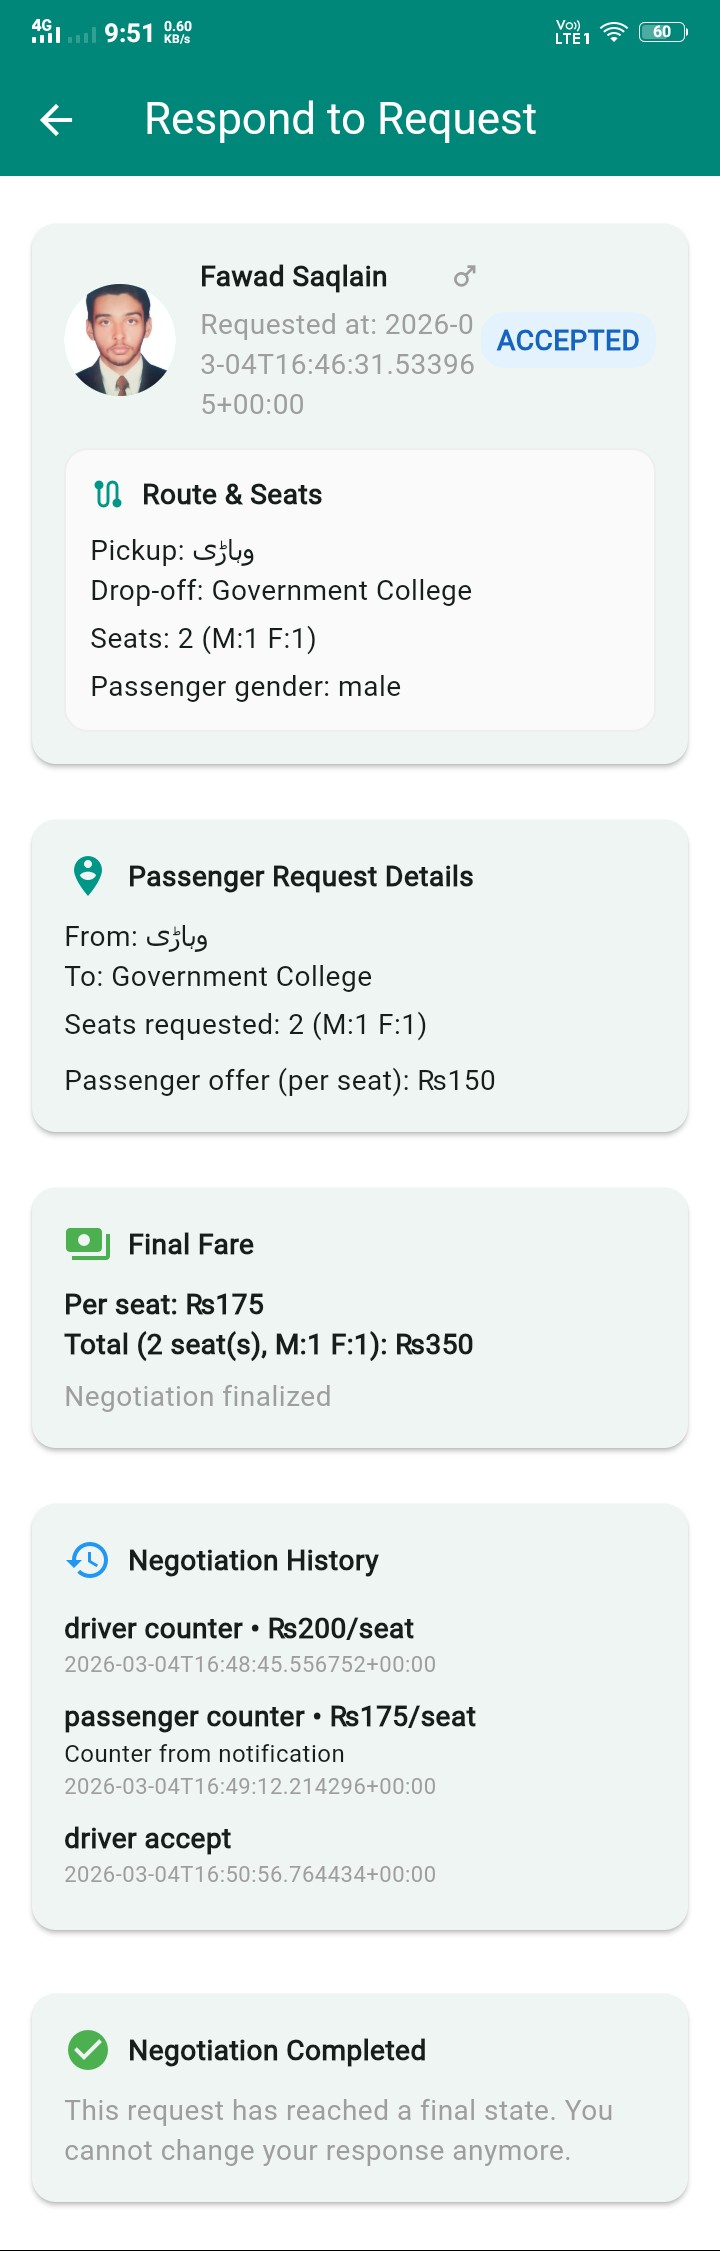
\includegraphics[width=\textwidth,height=0.65\textheight]{assets/app screenshot/driver_respond_request_accepted.jpeg}}
\end{minipage}\hfill
\begin{minipage}{0.45\textwidth}
\centering
\fbox{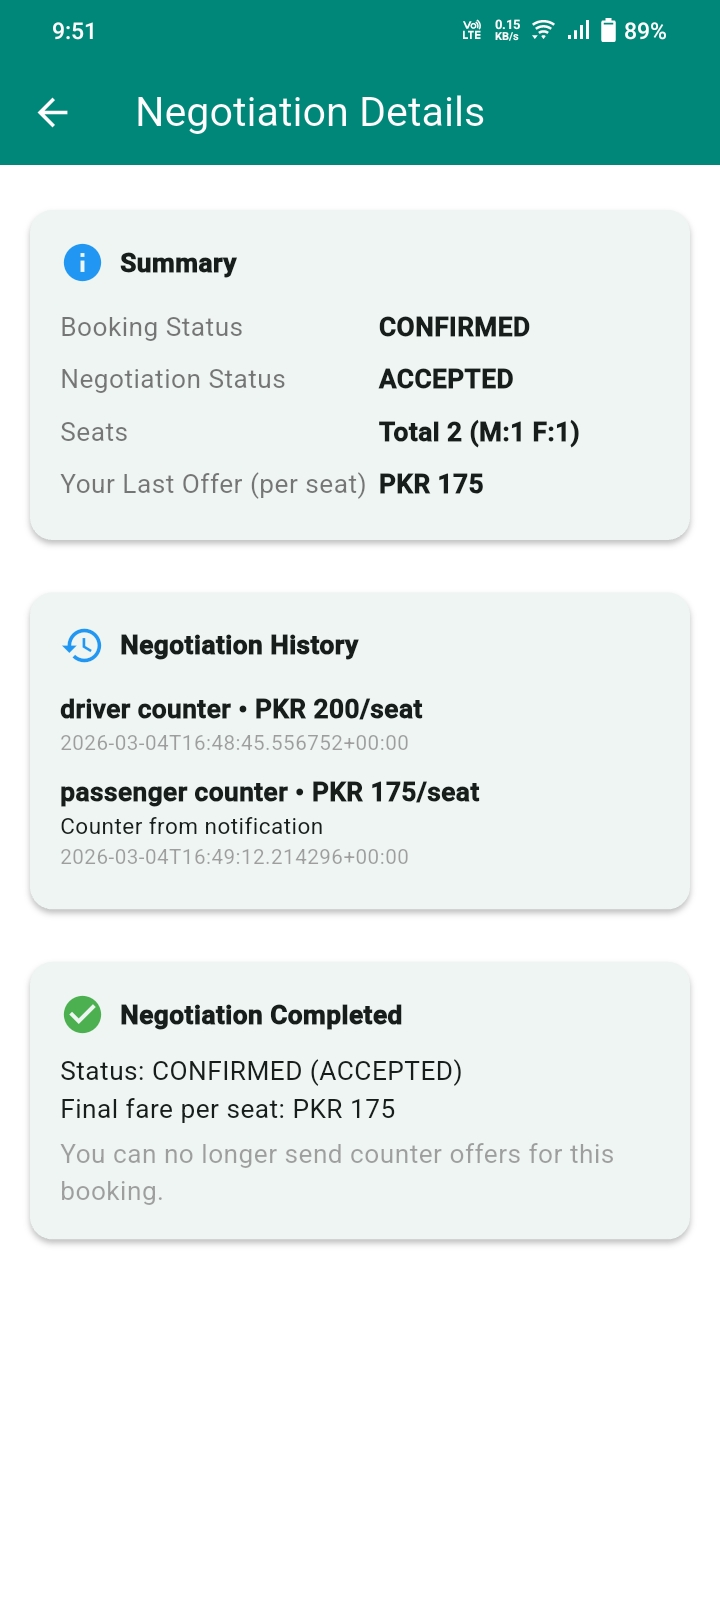
\includegraphics[width=\textwidth,height=0.65\textheight]{assets/app screenshot/passenger request accepted.jpg}}
\end{minipage}
\caption{Negotiation Completed}
\end{figure}

Accepted/Confirmed Booking: If both parties agree to the final terms, the booking moves to the accepted/confirmed state. The next steps open up – including chat, ride tracking, and, later, payments confirmation.

\textbf{Backend Integration:} When a user accepts it, it is stored in the booking and downstream (notifications, lock seats, etc. and tracking readiness of the session).

\textbf{Validation/Security:} Backend validates that acceptance may take place from valid negotiation states and from authorized users.

\subsubsection{Screen 24: My Rides}

\textbf{Function:} Providing users with a dashboard where they can view their future and current trips commitments.

\textbf{Components:}
\begin{itemize}
    \item Active ride cards with quick actions such as Chat and Tracking.
\end{itemize}

\begin{figure}[H]
\centering
\begin{minipage}{0.45\textwidth}
\centering
\fbox{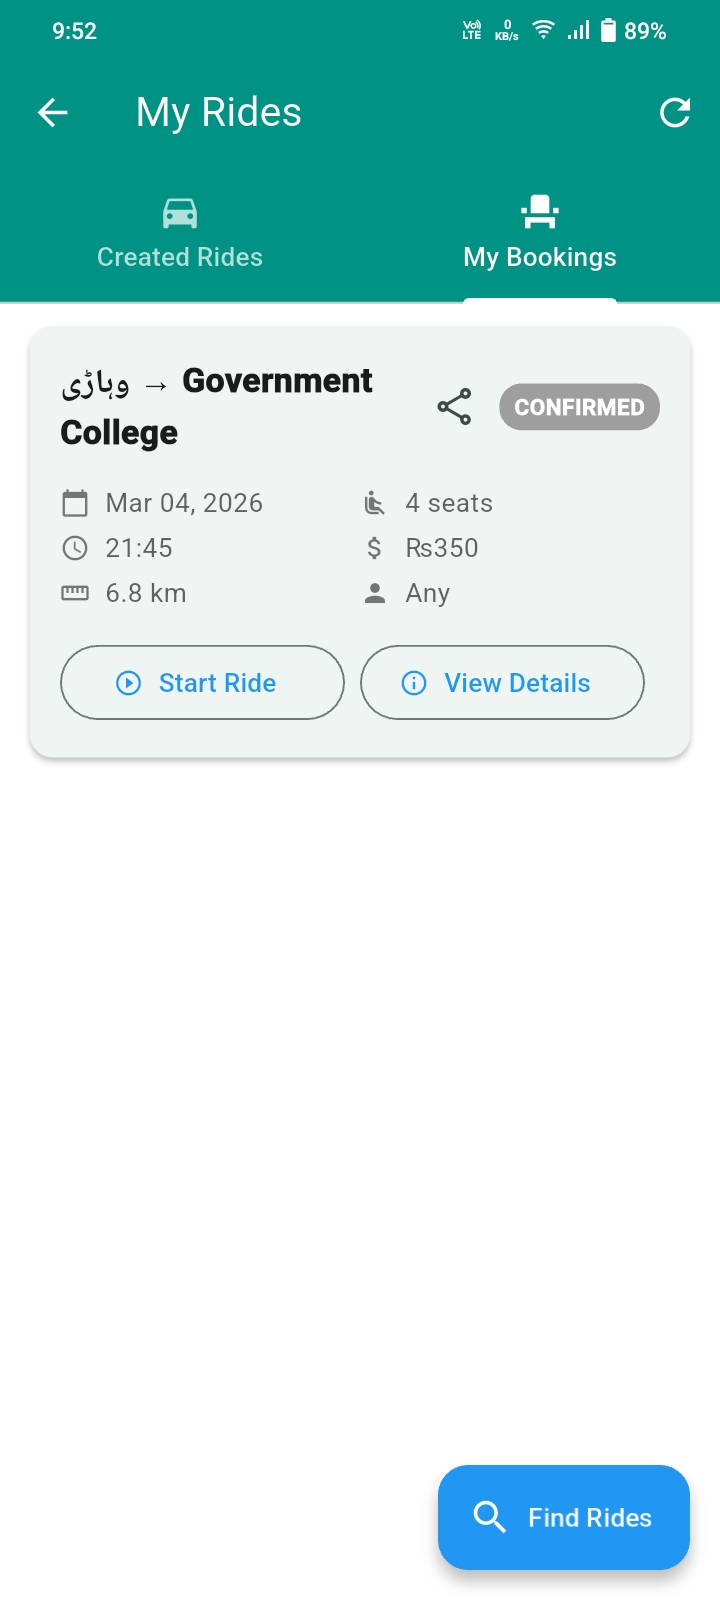
\includegraphics[width=\textwidth,height=0.65\textheight,keepaspectratio]{assets/app screenshot/my_bookings_confirmed.jpeg}}
\end{minipage}\hfill
\begin{minipage}{0.45\textwidth}
\centering
\fbox{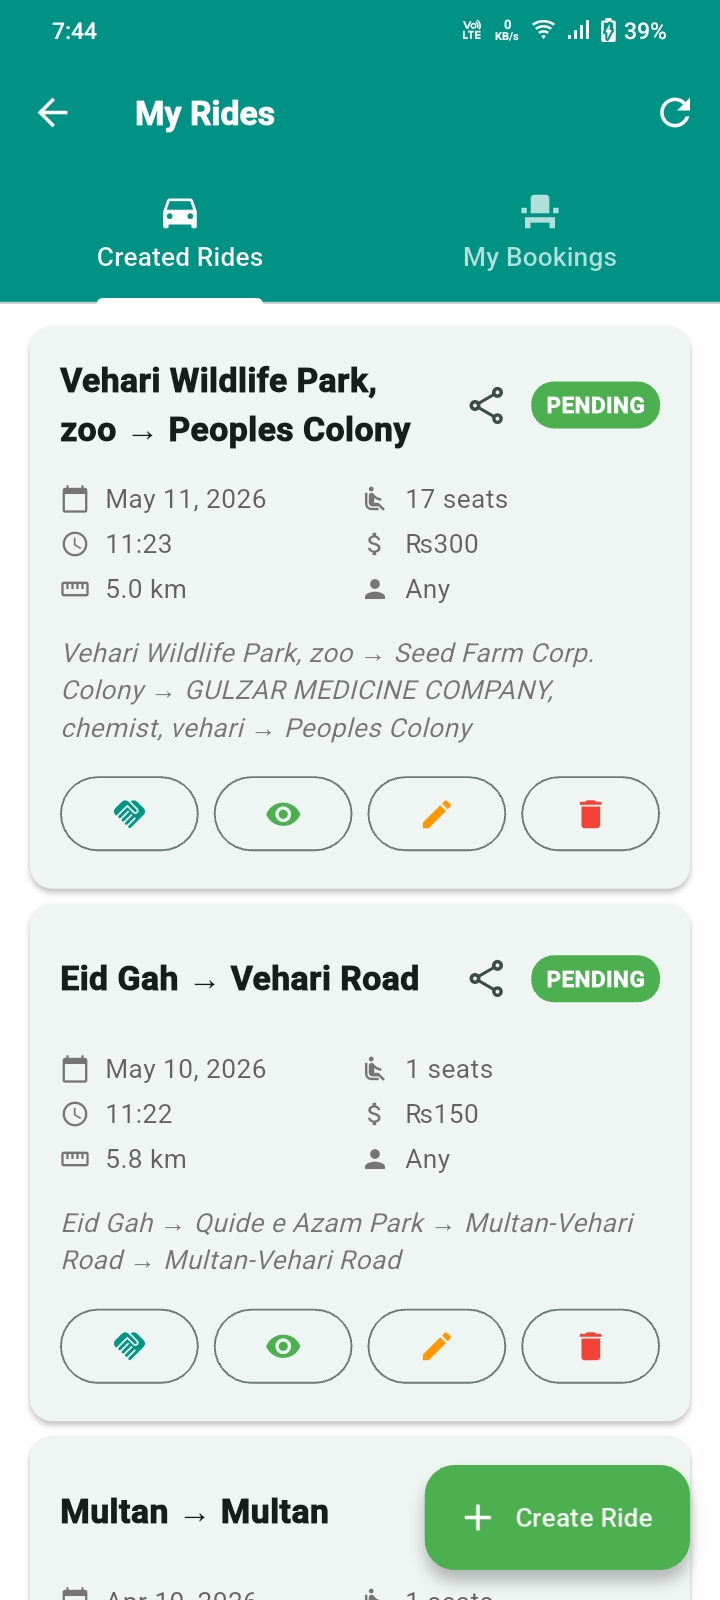
\includegraphics[width=\textwidth,height=0.65\textheight,keepaspectratio]{assets/app screenshot/my rides created rides.jpg}}
\end{minipage}
\caption{My Rides}
\end{figure}

The functional flow will let users see all their currently active and upcoming rides from one list and launch actions like chat, tracking etc. This screen is the primary one for post-booking operations.

\textbf{Backend Integration:} Fetches ride list from booking and trip history endpoints, and filters by status.

\textbf{Validation/Security:} Results are filtered for the authenticated user and sensitive data is obscured by roles.

\subsubsection{Screen 25: Live Tracking and Pickup Verification}

This screen provides live tracking and pick-up verification.This screen offers live tracking and pick-up verification.

\textbf{Goal:} Real time monitoring of an active ride for driver and passenger, secure pickup verification.

\textbf{Components:}
\begin{itemize}
    \item GPS Markers for vehicle and pickup location.
    \item Periodic ETA updates.
    \item QR Code verification for pickups.
\end{itemize}

\begin{figure}[H]
\centering
\begin{minipage}{0.30\textwidth}
\centering
\fbox{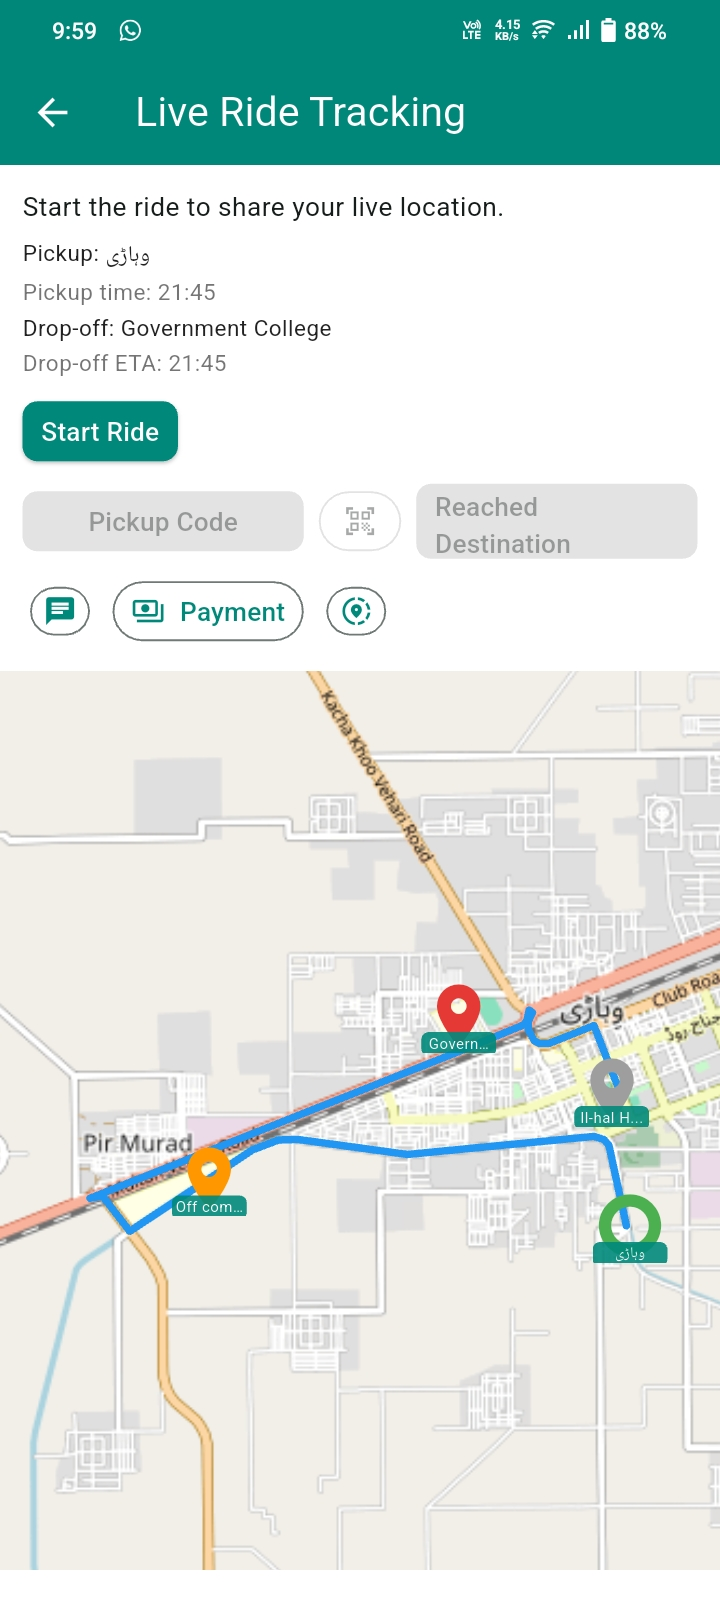
\includegraphics[width=\textwidth,keepaspectratio]{assets/app screenshot/passenger_live_tracking_start.jpeg}}
\end{minipage}\hfill
\begin{minipage}{0.30\textwidth}
\centering
\fbox{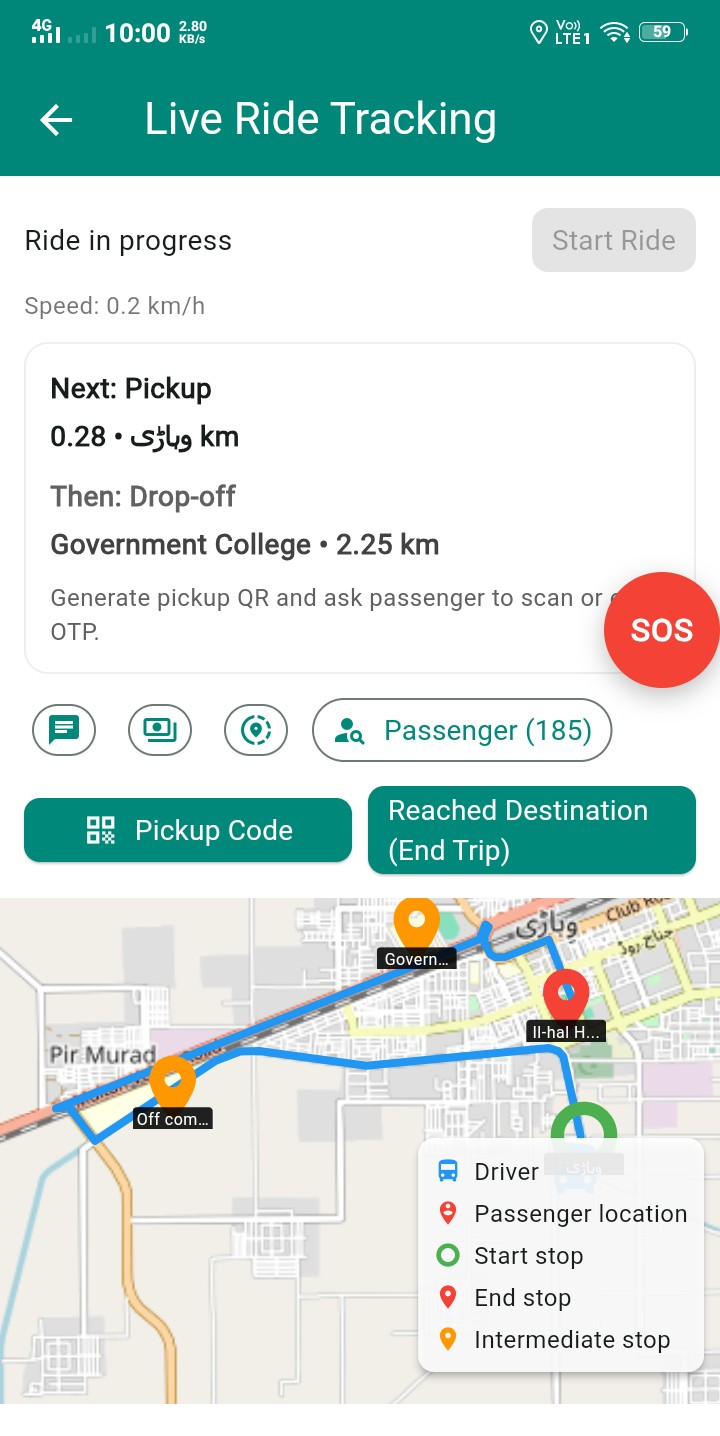
\includegraphics[width=\textwidth,keepaspectratio]{assets/app screenshot/driver_live_ride_tracking.jpeg}}
\end{minipage}\hfill
\begin{minipage}{0.30\textwidth}
\centering
\fbox{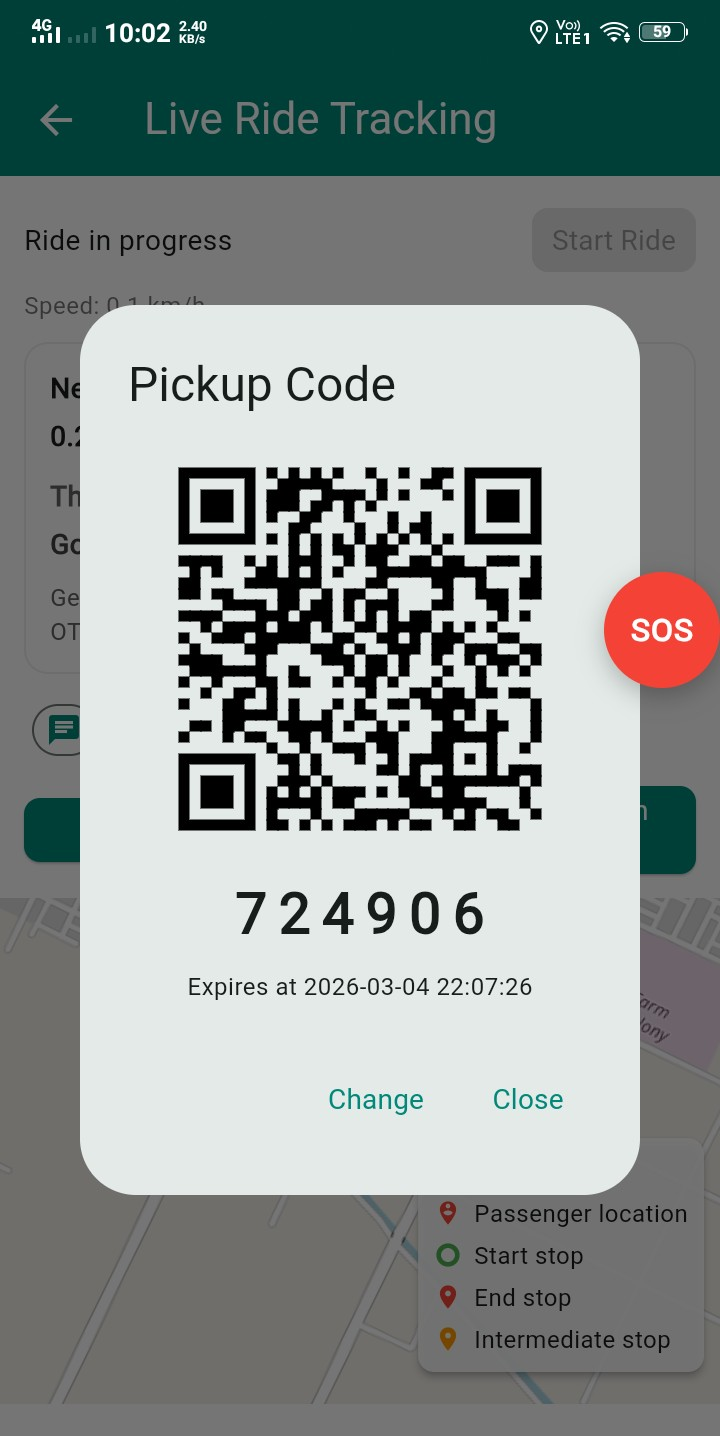
\includegraphics[width=\textwidth,keepaspectratio]{assets/app screenshot/driver_pickup_qr_code.jpeg}}
\end{minipage}
\caption{Passenger Live Tracking, Driver Live Tracking, and Driver Pickup QR Code}
\end{figure}

Figure 5.13 is a passenger live tracking, driver live tracking, and driver pick up QR code.

The QR code is checked for boarding at pickup before heading on to the process.

\textbf{Tracking:} Periodic location updates through API calls and bookings and trip identifier to get the live state of the session.

\textbf{Validation/Security:} Only users on the active booking can access the tracking, pickup verification prevents unauthorized boarding.

\subsubsection{Screen 29: Payment and Rating Screen}

The Payment and Rating Screen opens.The Payment and Rating screen appears.

\textbf{Use:} Allows riders to pay, rate after a ride and for the driver to acknowledge receipt of payment.

\textbf{Components:}
\begin{itemize}
    \item Choice and confirmation of payment method and final amount.
    \item Submitting a rating following payment.
    \item Receipt confirmation on driver.
\end{itemize}

\begin{figure}[H]
\centering
\begin{minipage}{0.30\textwidth}
\centering
\fbox{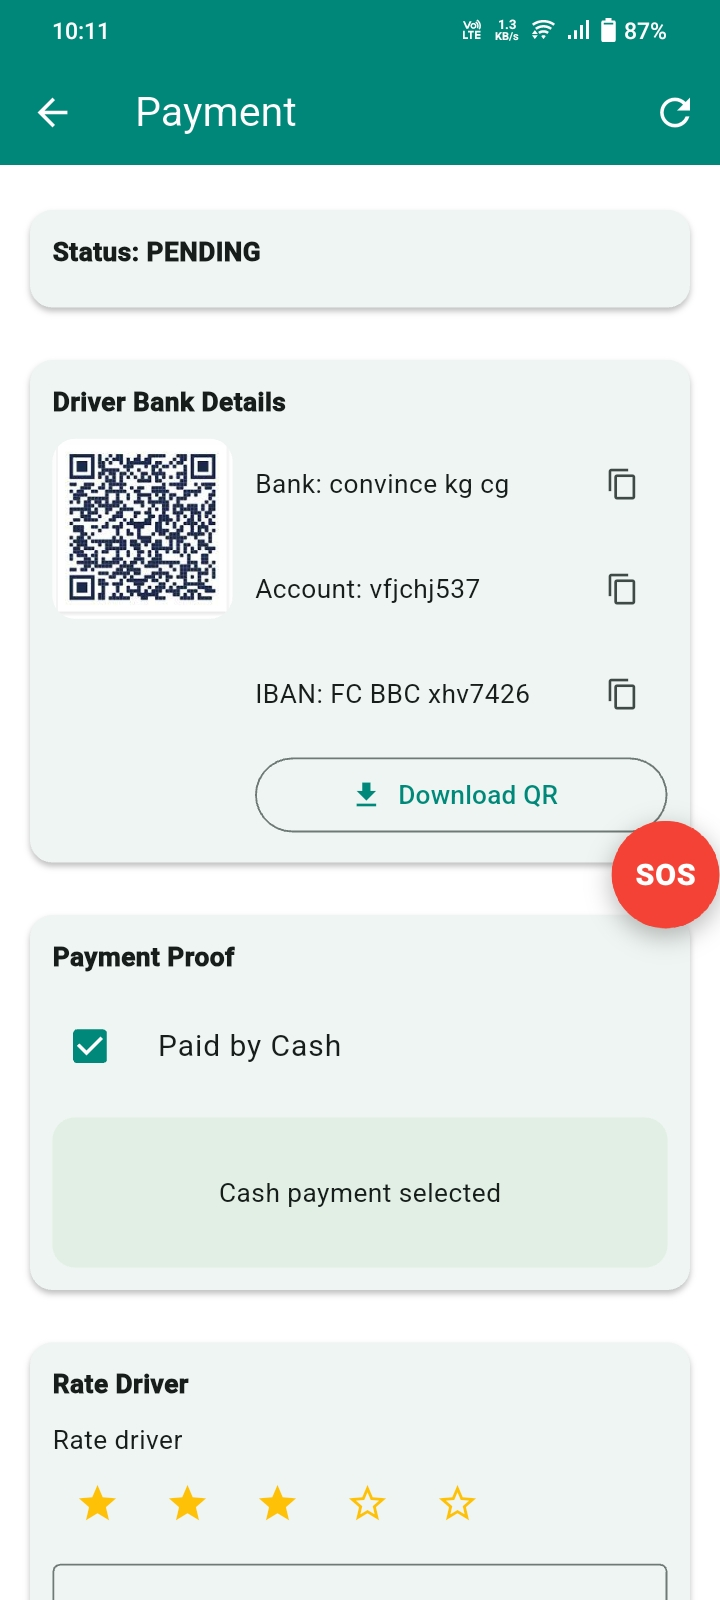
\includegraphics[width=\textwidth,keepaspectratio]{assets/app screenshot/payment_screen_cash.jpeg}}
\end{minipage}\hfill
\begin{minipage}{0.30\textwidth}
\centering
\fbox{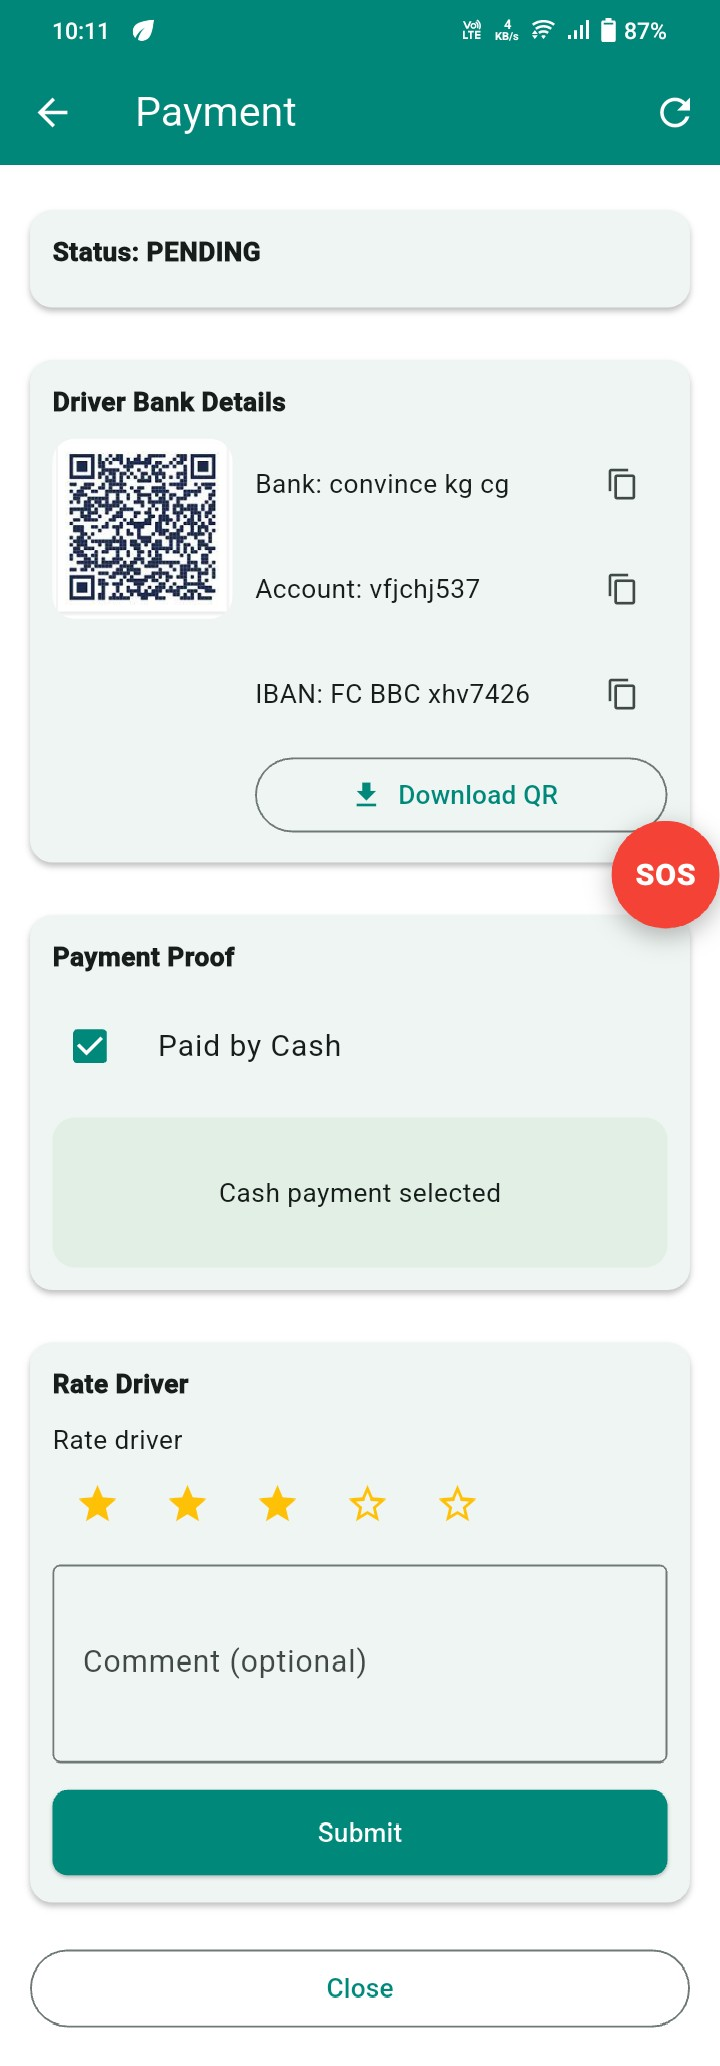
\includegraphics[width=\textwidth,height=0.55\textheight]{assets/app screenshot/passenger payment and rating screen.jpeg}}
\end{minipage}\hfill
\begin{minipage}{0.30\textwidth}
\centering
\fbox{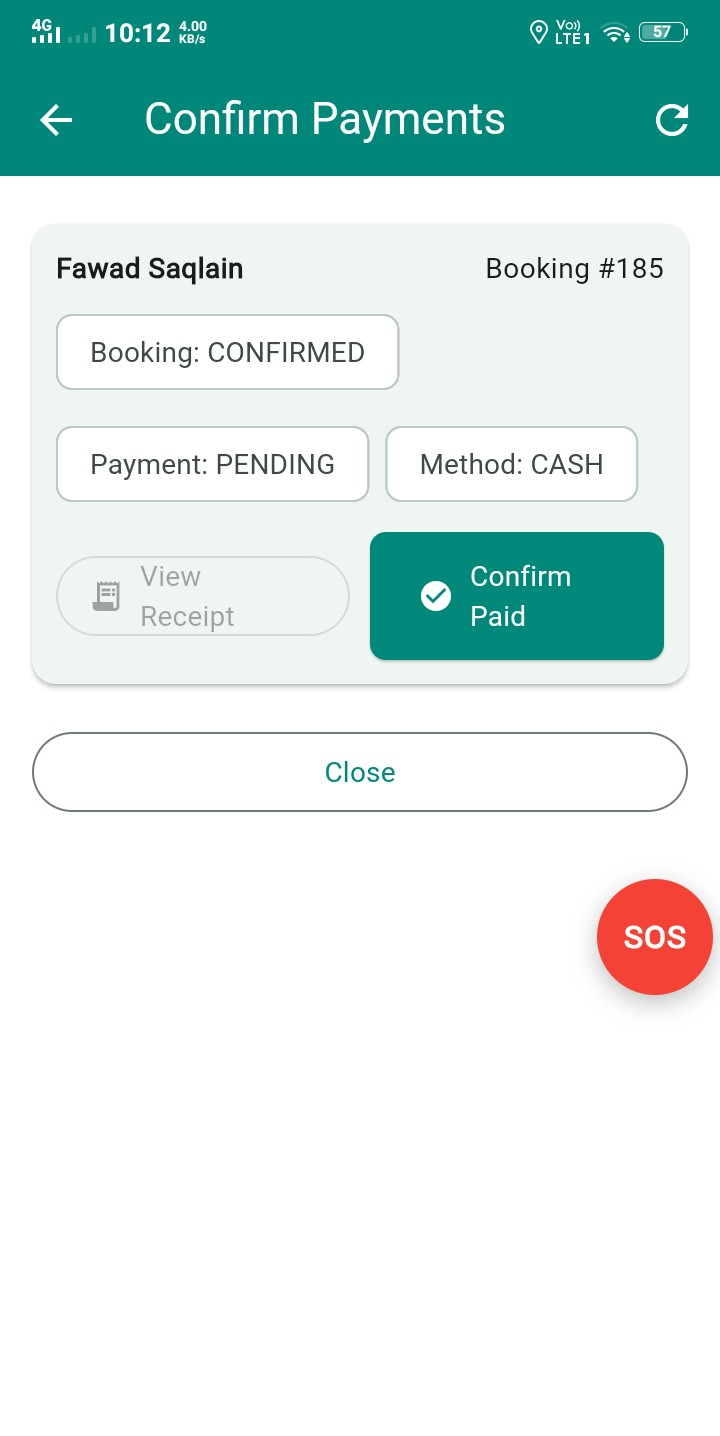
\includegraphics[width=\textwidth,keepaspectratio]{assets/app screenshot/driver_confirm_payments.jpeg}}
\end{minipage}
\caption{Passenger Payment, Rating, and Driver Payment Confirmation}
\end{figure}

Once the driver has confirmed receipt, the booking is complete.

\textbf{Backend Integration:} Payment submit / payment confirm endpoints that are coupled to the booking/payment records.

\textbf{Validation/Security:} Confirmation permissions are role based and there is no double confirmation.

\subsubsection{Screen 31: Messaging and User Chat}

Messaging and User Chat:Screen 31: Messaging and User Chat:

The purpose is to provide unified communication system for drivers to communicate with passengers.

\textbf{Components:}
\begin{itemize}
    \item Bubble chat where bubbles are marked with a time.
\end{itemize}

\begin{figure}[H]
\centering
\begin{minipage}{0.30\textwidth}
\centering
\fbox{
\includegraphics[width=\textwidth,keepaspectratio]{assets/app screenshot/driver_trip_passengers_list.jpeg}}
\end{minipage}\hfill
\begin{minipage}{0.30\textwidth}
\centering
\fbox{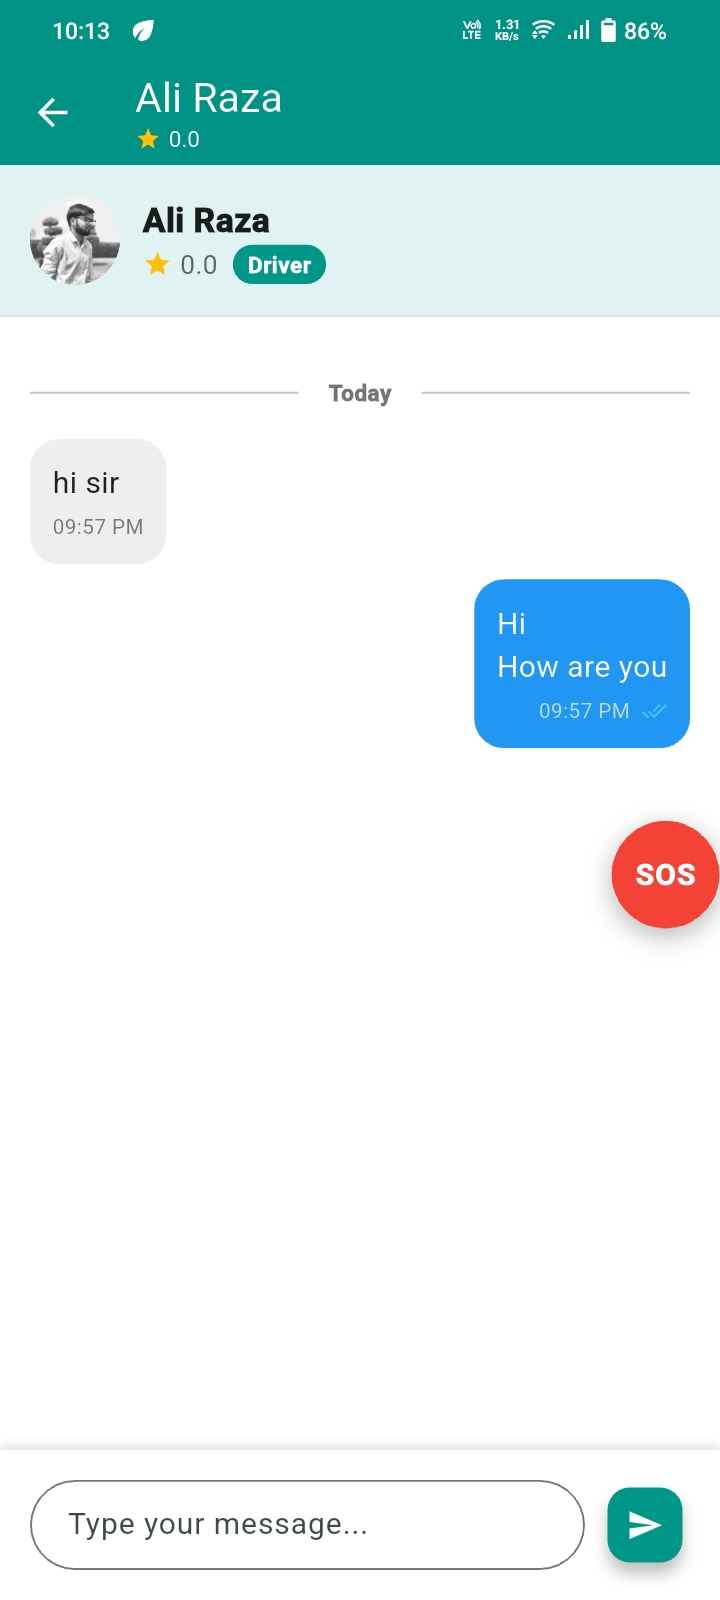
\includegraphics[width=\textwidth,keepaspectratio]{assets/app screenshot/passenger_driver_one_to_one_chating_screen.jpeg}}
\end{minipage}\hfill
\begin{minipage}{0.30\textwidth}
\centering
\fbox{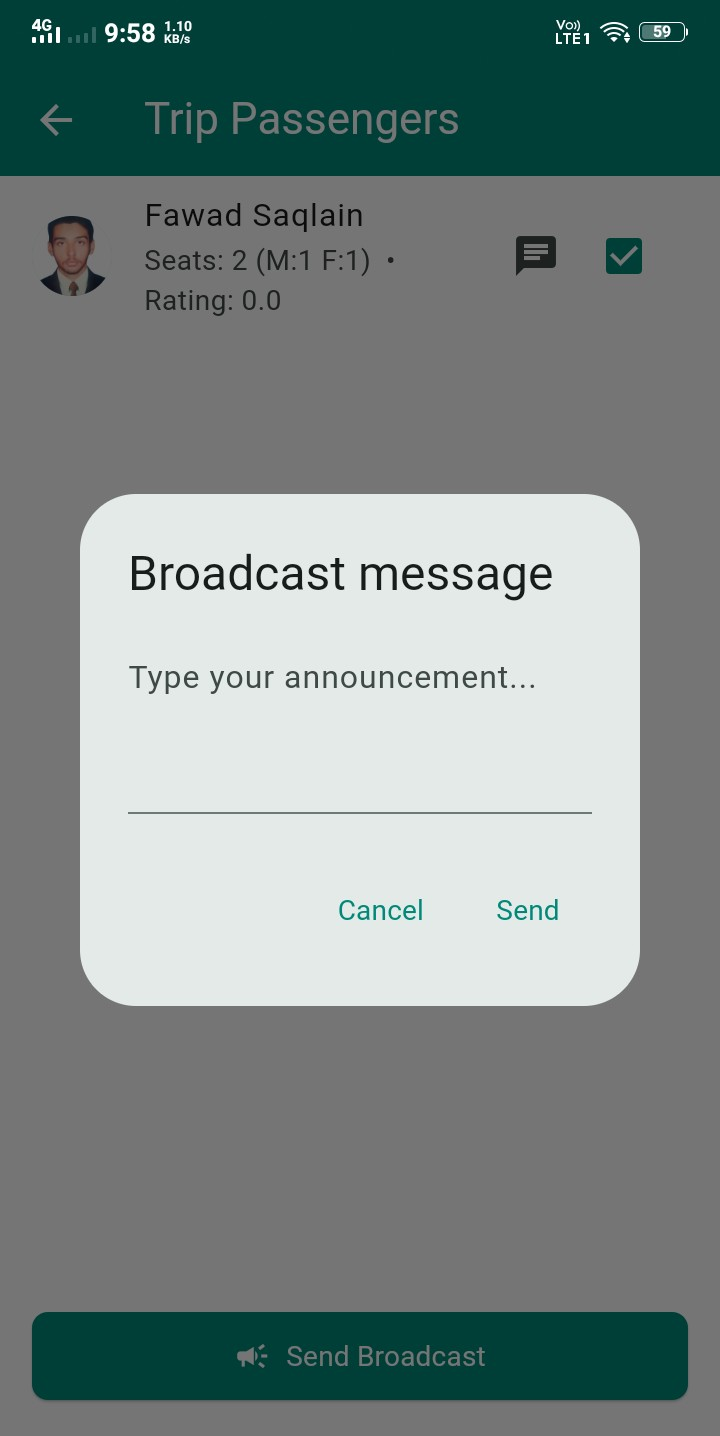
\includegraphics[width=\textwidth,keepaspectratio]{assets/app screenshot/driver_broadcast_message.jpeg}}
\end{minipage}
\caption{Messaging and User Chat}
\end{figure}

Booking and ride execution involves functional flow: Drivers and passengers are exchanging messages for coordination and updates. Broadcast messages can be used to send information to ALL passengers on a trip.

\textbf{Backend Integration:} Messaging stores messages for future retrieval and does so through chat service endpoints.

\textbf{Validation/Security:} Messages can only be seen by participants in the same trip/booking, and message filters are based on the roles of the participants.

\subsubsection{Screen 32: Support Chat - Bot \& Admin}

On screen \#32, you can click on the Support Chat-Bot \& Admin button.Click Support Chat-Bot \& Admin on screen \#32.

\textbf{Goal:} A dedicated channel for platform support and manual resolution.

\textbf{Components:}
\begin{itemize}
    \item Bot response options and live Admin escalation.
\end{itemize}

\begin{figure}[H]
\centering
\begin{minipage}{0.45\textwidth}
\centering
\fbox{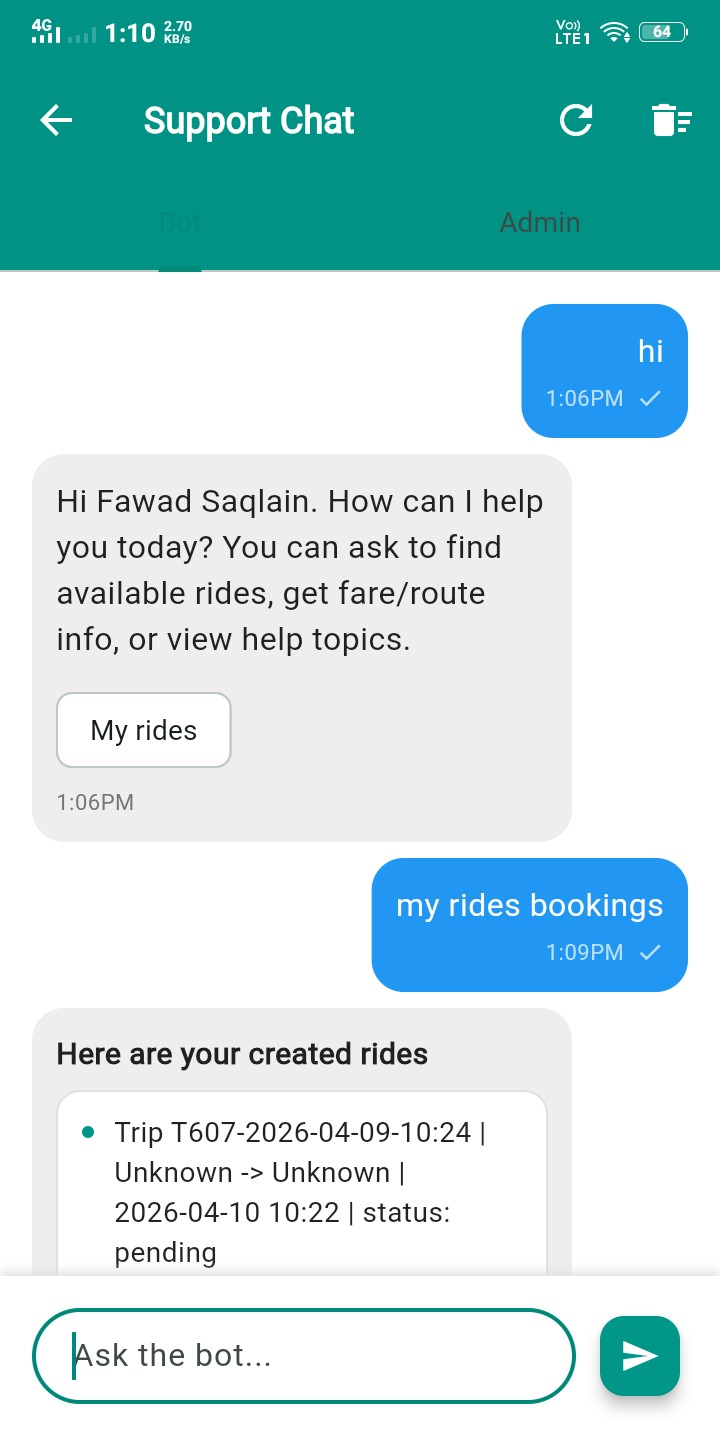
\includegraphics[width=\textwidth,keepaspectratio]{assets/app screenshot/support_chat_bot.jpeg}}
\end{minipage}\hfill
\begin{minipage}{0.45\textwidth}
\centering
\fbox{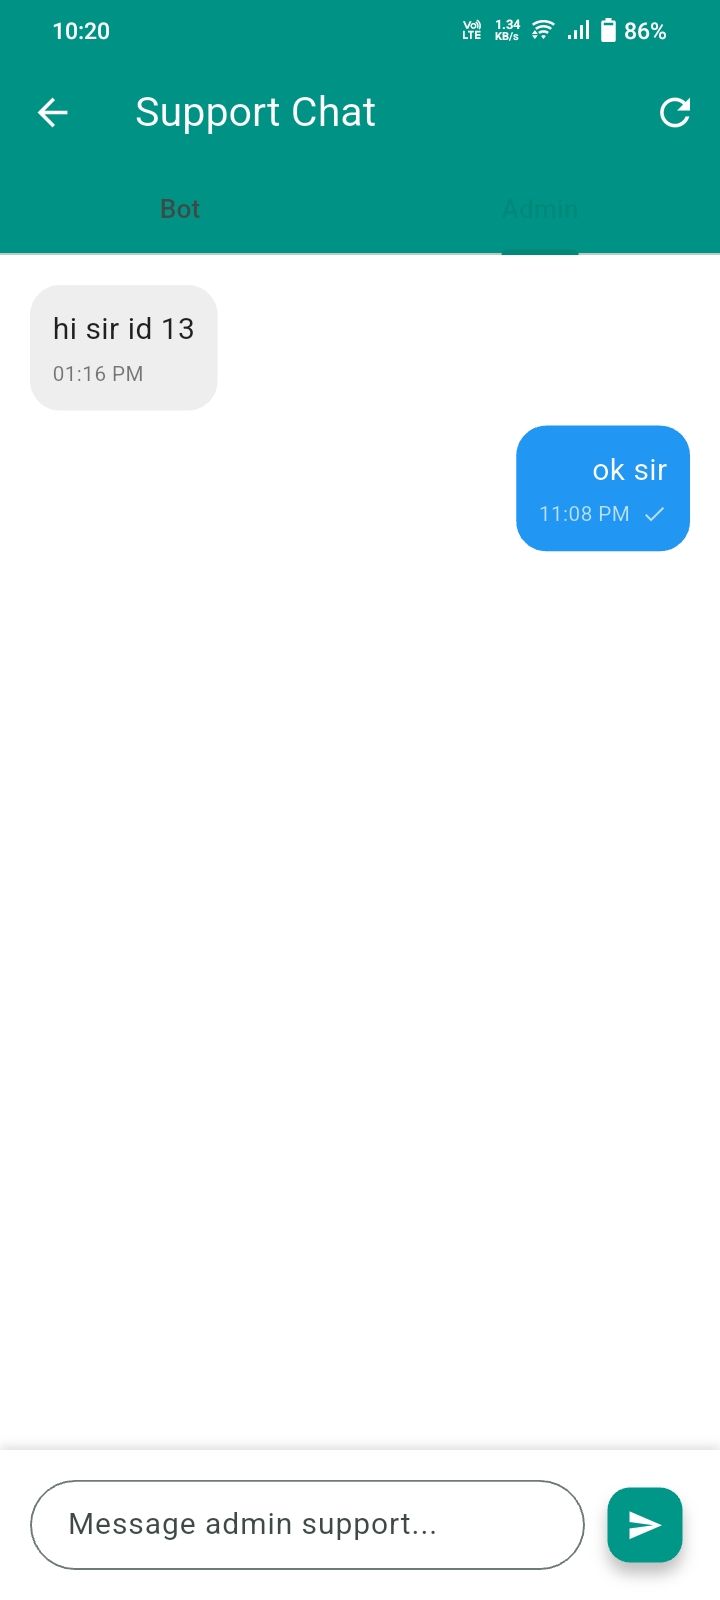
\includegraphics[width=\textwidth,keepaspectratio]{assets/app screenshot/support_chat_admin_reply.jpeg}}
\end{minipage}
\caption{Support Chat - Bot \& Admin}
\end{figure}

The user first contacts the support bot to resolve common issues and guided troubleshooting. If it is a manual handling problem, it is discussed in an Admin support channel to resolve the issue.

\textbf{Backend Integration:} The screen loads and posts messages with support chat endpoints, and fetches new replies periodically.

\textbf{Validation/Security:} access restricted to authenticated user (or guest support session) and message threads (chats) isolated per user.

\subsubsection{Screen 33: Notifications List}

\textbf{Description:} All System Alerts for all Users are fed in chronological order.

\textbf{Components:}
\begin{itemize}
    \item Deep link notification cards.
\end{itemize}

\begin{figure}[H]
\centering
\begin{minipage}{0.45\textwidth}
\centering
\fbox{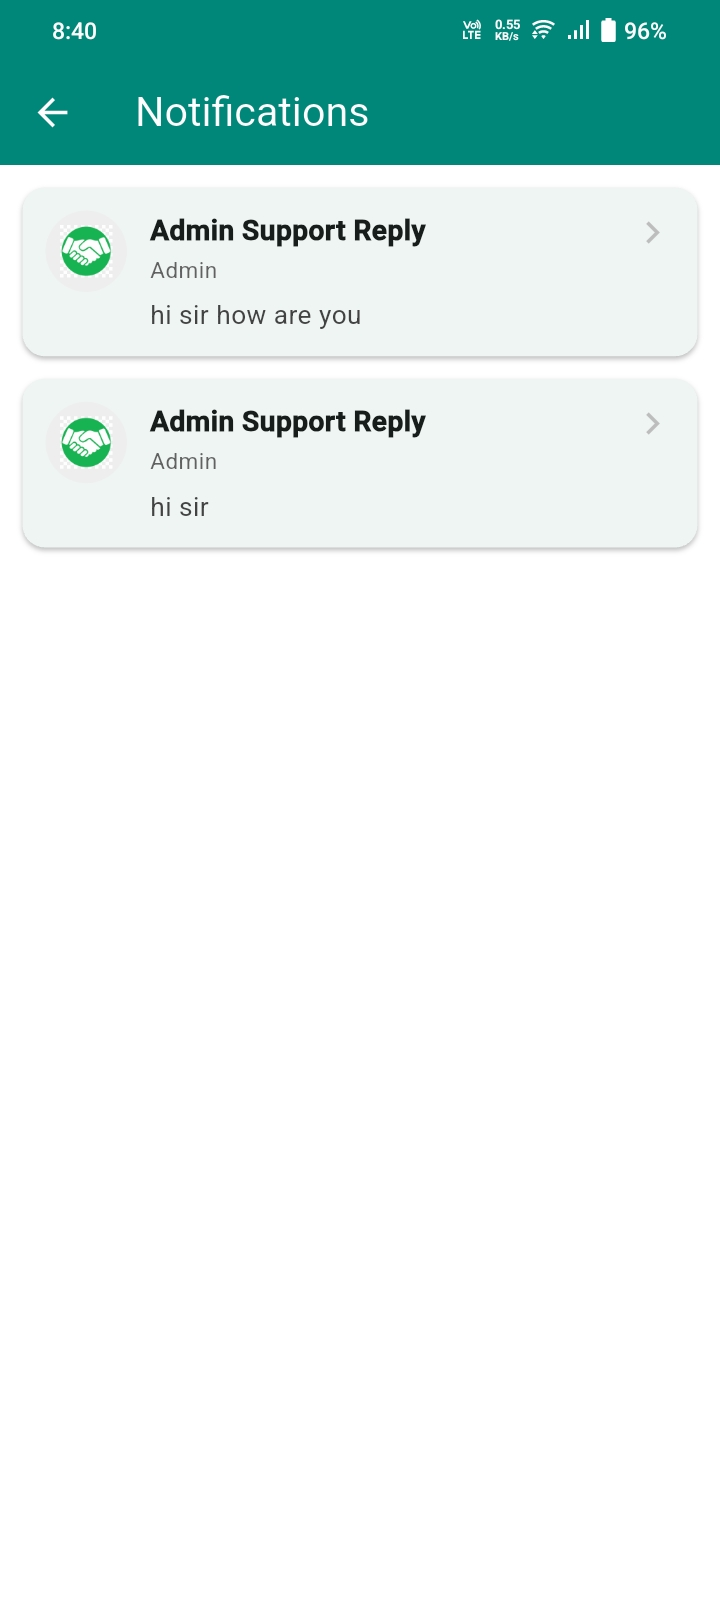
\includegraphics[width=\textwidth,height=0.66\textheight,keepaspectratio]{assets/app screenshot/notifications_list.jpeg}}
\end{minipage}\hfill
\begin{minipage}{0.45\textwidth}
\centering
\fbox{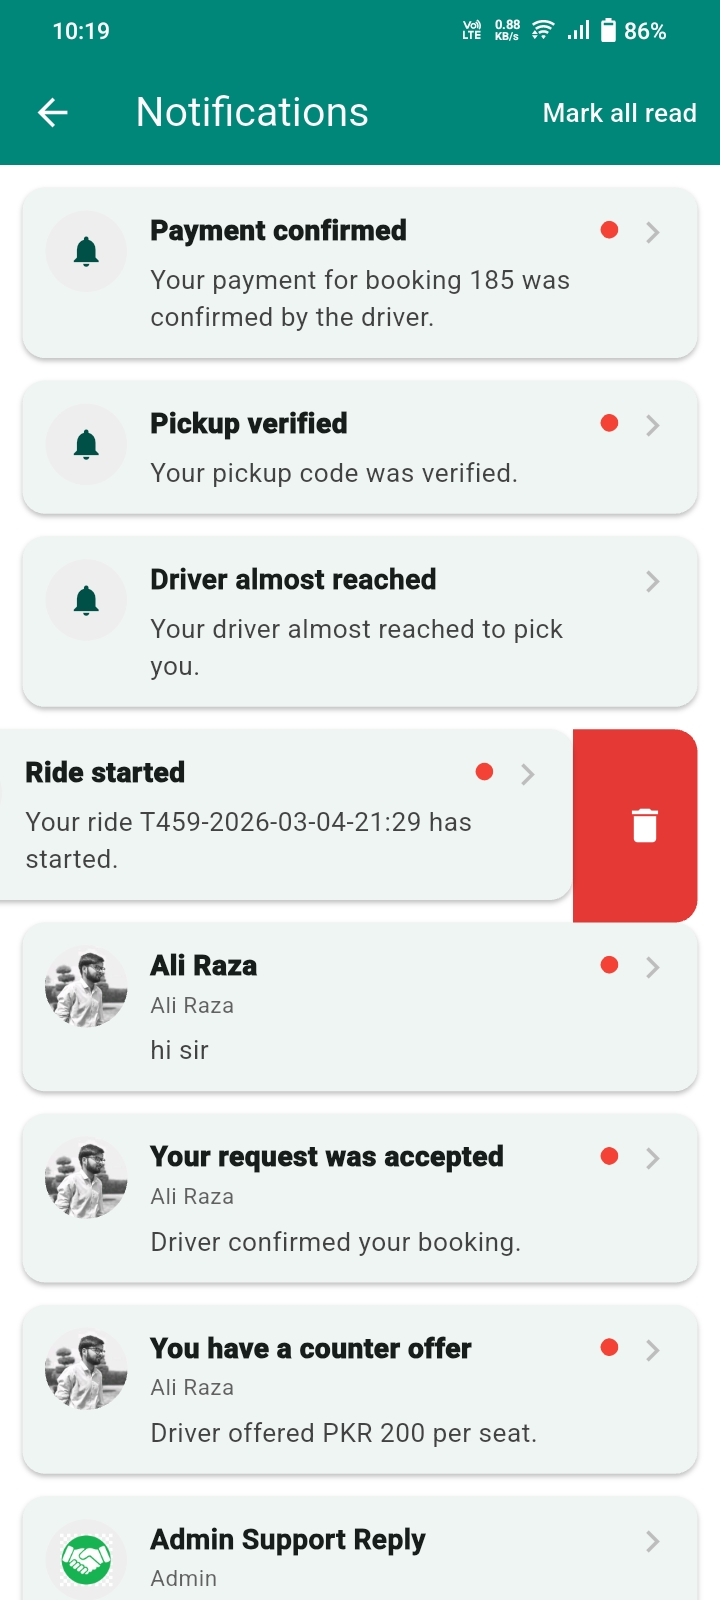
\includegraphics[width=\textwidth,height=0.66\textheight,keepaspectratio]{assets/app screenshot/notification_deletion.jpeg}}
\end{minipage}
\caption{Notifications List}
\end{figure}

Functional Flow: User opens the notifications inbox to check updates on booking, SOS alerts, and system announcements. Deep-links direct users to the relevant screen and notifications can be viewed and dismissed.

\textbf{Backend Integration:} Notifications are retrieved from the backend notifications API and refreshed periodically, or when triggered by FCM.

\textbf{Validation/Security:} Only the current user's notifications returned and sensitive payload data filtered by role and ownership.

\subsubsection{Screen 34-35: Emergency SOS}

The purpose is to provide intervener to user with tool to intervene in the immediate moment of distress.

\textbf{Components:}
\begin{itemize}
    \item Visual confirmation of countdown and alarm.
\end{itemize}

\begin{figure}[H]
\centering
\begin{minipage}{0.30\textwidth}
\centering
\fbox{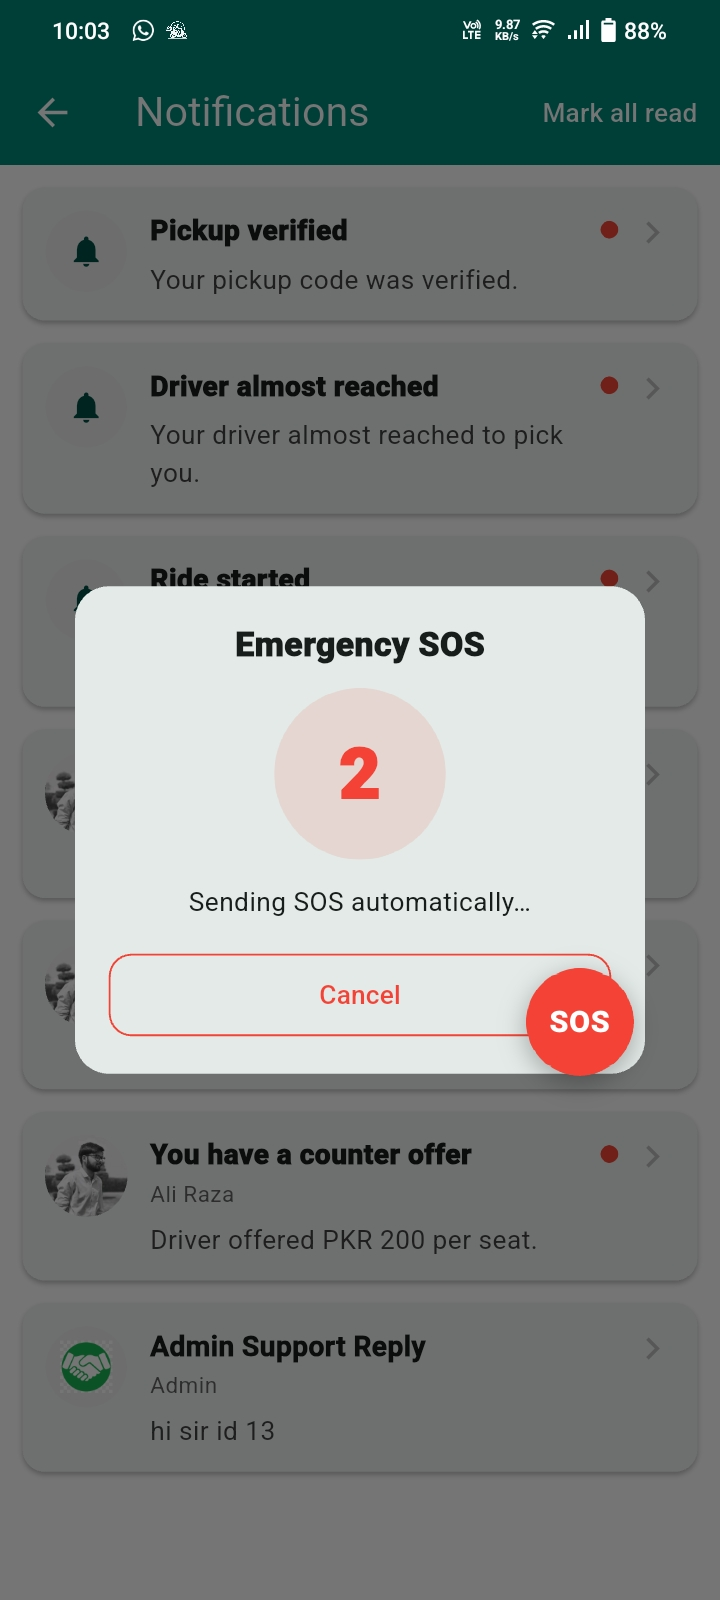
\includegraphics[width=\textwidth,keepaspectratio]{assets/app screenshot/emergency_sos_countdown.jpeg}}
\end{minipage}\hfill
\begin{minipage}{0.30\textwidth}
\centering
\fbox{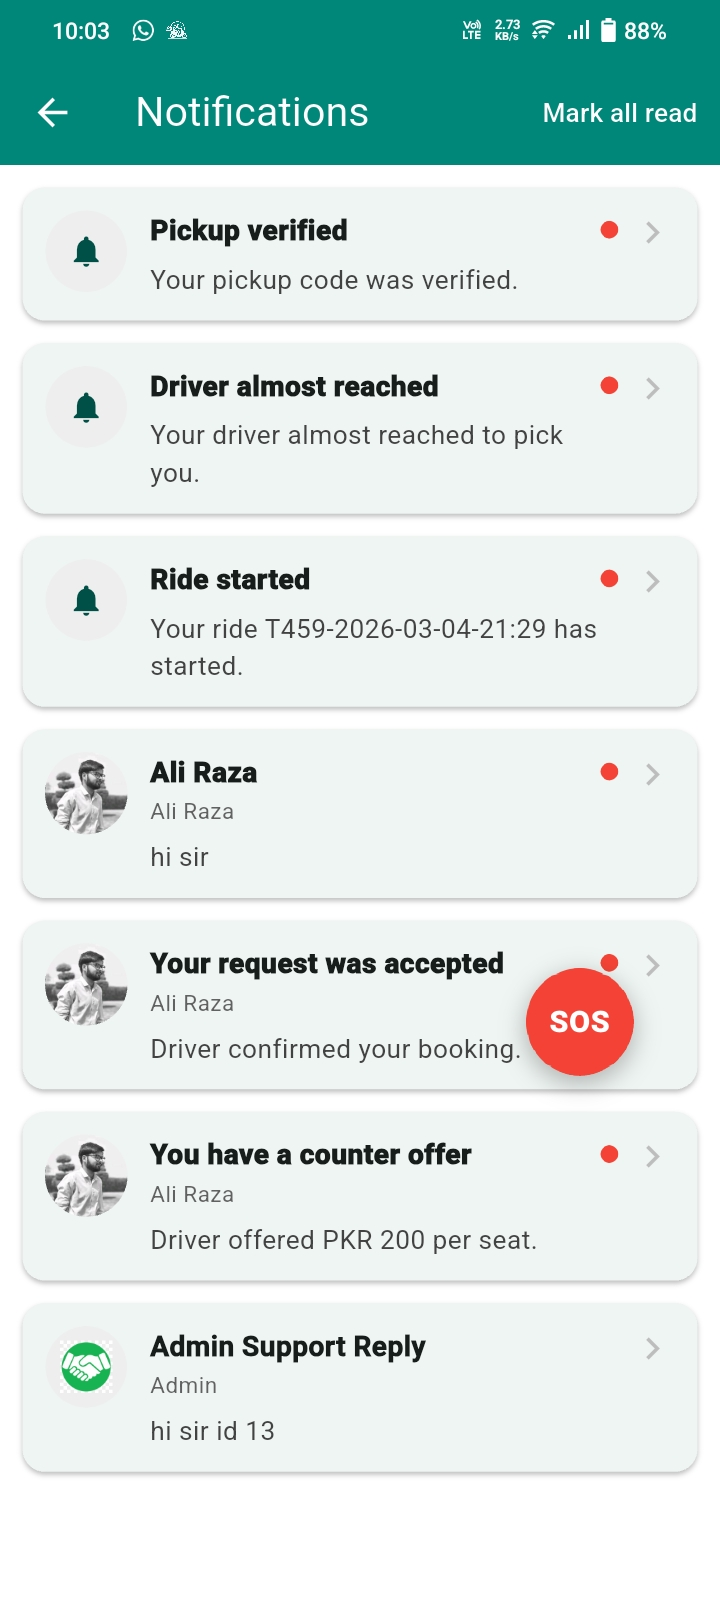
\includegraphics[width=\textwidth,keepaspectratio]{assets/app screenshot/notifications_list_sos.jpeg}}
\end{minipage}\hfill
\begin{minipage}{0.30\textwidth}
\centering
\fbox{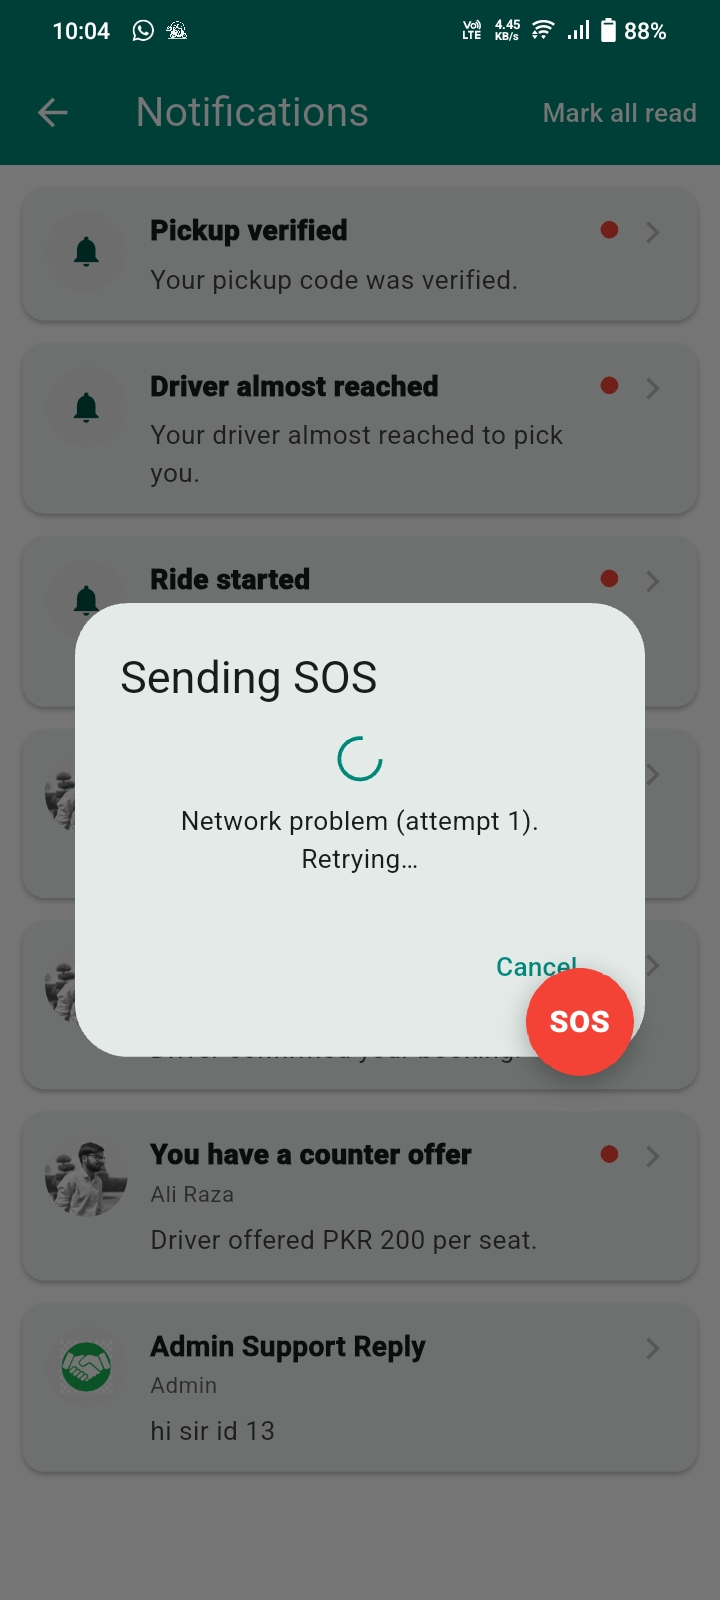
\includegraphics[width=\textwidth,keepaspectratio]{assets/app screenshot/emergency_sos_network_error.jpeg}}
\end{minipage}
\caption{Emergency SOS (Countdown, SOS Notifications, and Offline/Error State)}
\end{figure}

Functional Flow: User activates SOS, goes through the countdown confirmation, and the incident is documented and reported via SOS notifications. If there is an offline/connection error, the UI gives the user offline/connection advice until the request can be made.

\textbf{Backend Integration:} SOS events are sent to the back-end incident endpoints, and trigger notification entries to users and Admin monitoring.

\textbf{Validation/Security:} Requests for SOS are associated with the current session user, and subjected to rate limits, thereby preventing abuse; visibility of incidents are role-controlled.

\subsubsection{Screen 36: Profile Overview}

\textbf{Purpose:} Manage personal stats and application settings.

\textbf{Components:}
\begin{itemize}
    \item User profile card and navigation menu.
\end{itemize}

\begin{figure}[H]
\centering
\begin{minipage}{0.45\textwidth}
\centering
\fbox{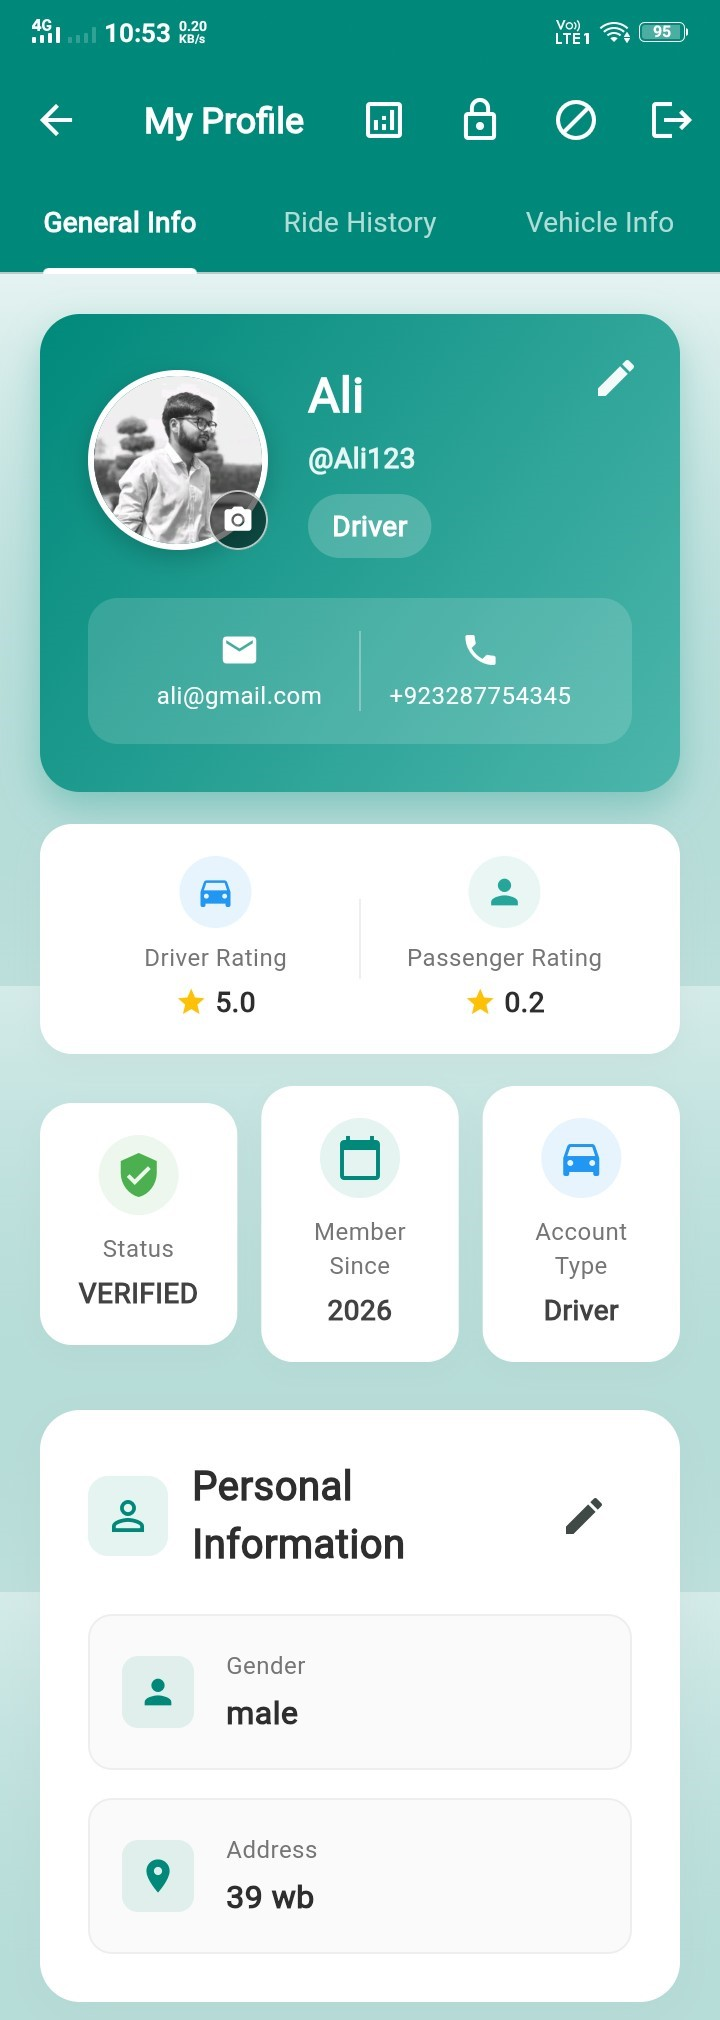
\includegraphics[width=\textwidth,height=0.8\textheight,keepaspectratio]{assets/app screenshot/profile_general_info_part1.jpeg}}
\end{minipage}\hfill
\begin{minipage}{0.45\textwidth}
\centering
\fbox{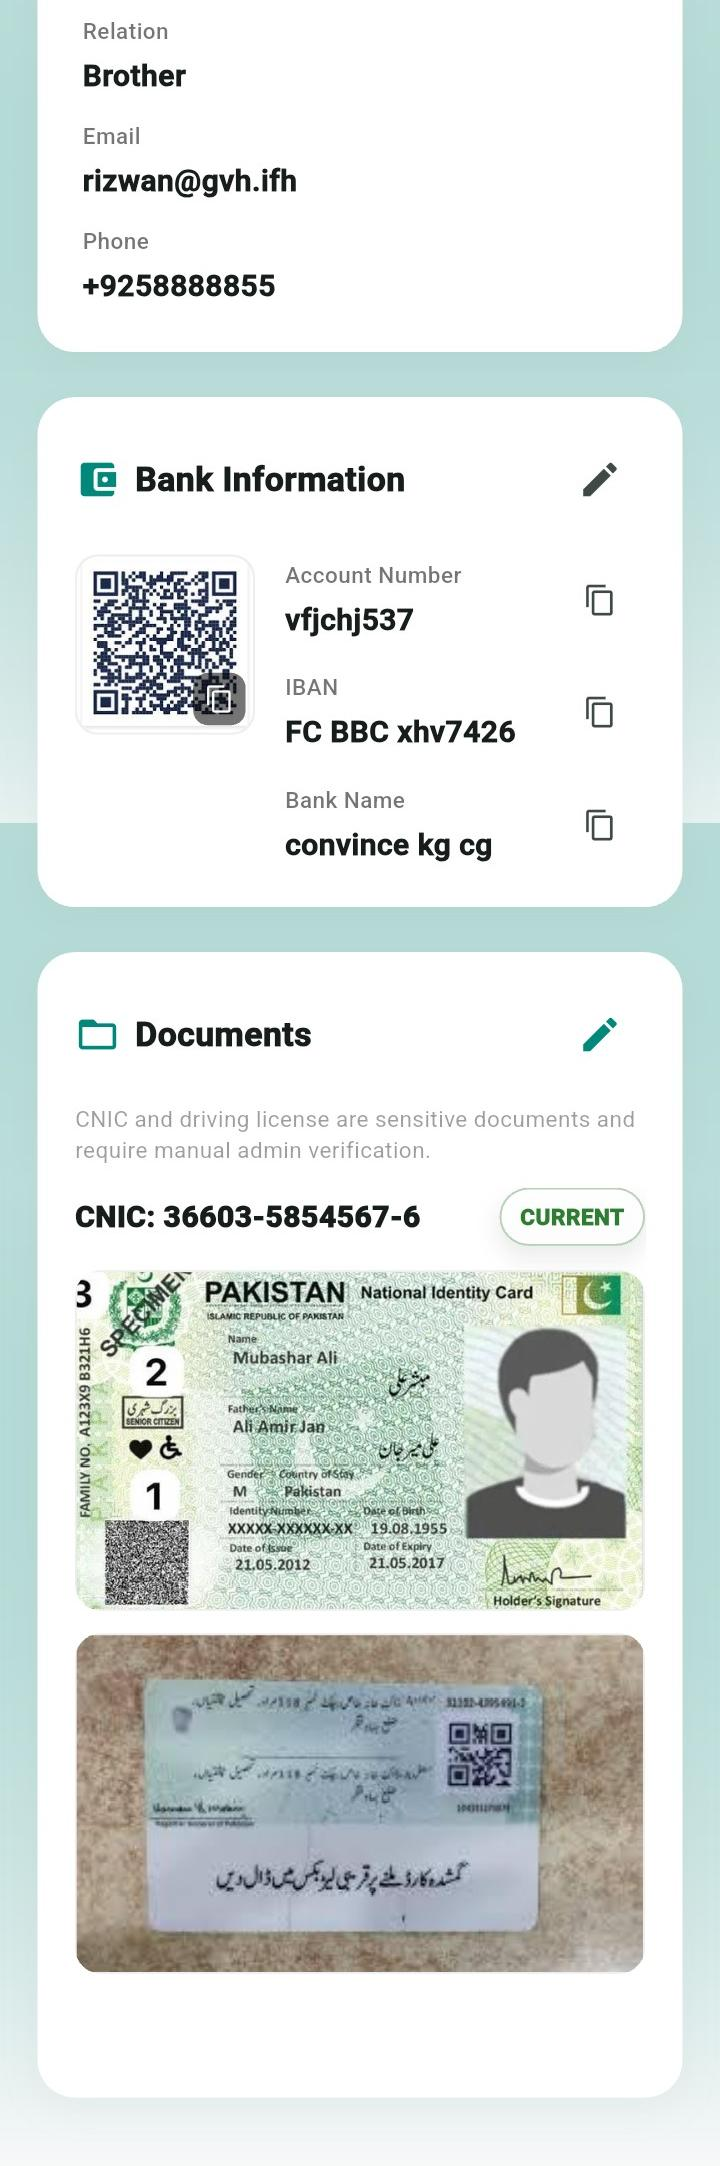
\includegraphics[width=\textwidth,height=0.8\textheight,keepaspectratio]{assets/app screenshot/profile_general_info_part2.jpeg}}
\end{minipage}
\caption{Profile Overview}
\end{figure}

Functional Flow: User accesses profile information, and accesses other linked areas like analytics, ride history, blocked users. Profile actions update the local state and instantaneously after successful backend updates.

\textbf{Backend Integration:} Profile data is retrieved from user profile endpoints and updated (e.g., edited) by authenticated API calls.

\textbf{Validation/Security:} edit must be authenticated, input validated before submission, and role checks for driver-only settings.

\subsubsection{Screen 37: Profile Analytics}

Purpose: Gives the user a combined overview of their riding history in the past.

Description: The screen includes time-based filtering (All-time, last 30 days, last 7 days) and provides key indicators for both driver and passenger positions. It provides a summary of created/booked rides, completion rates, distance covered and spending/revenue. Trend charts are used to show revenue and expenditures over time and a note box alerts the reader to possible data delays.

\begin{figure}[H]
\centering
\begin{minipage}{0.45\textwidth}
\centering
\fbox{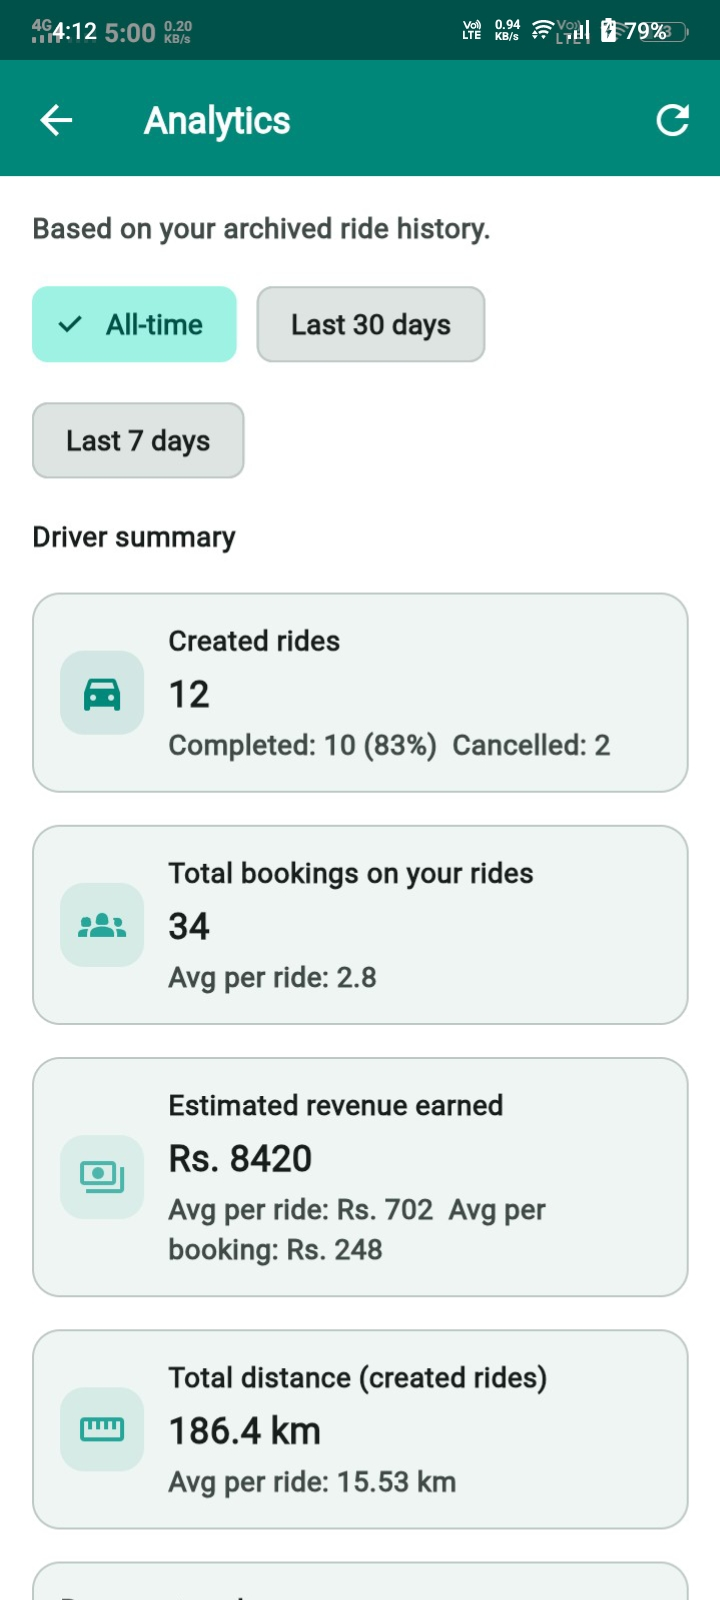
\includegraphics[width=\textwidth,height=0.6\textheight,keepaspectratio]{assets/app screenshot/analytics_part_1.jpeg}}
\end{minipage}\hfill
\begin{minipage}{0.45\textwidth}
\centering
\fbox{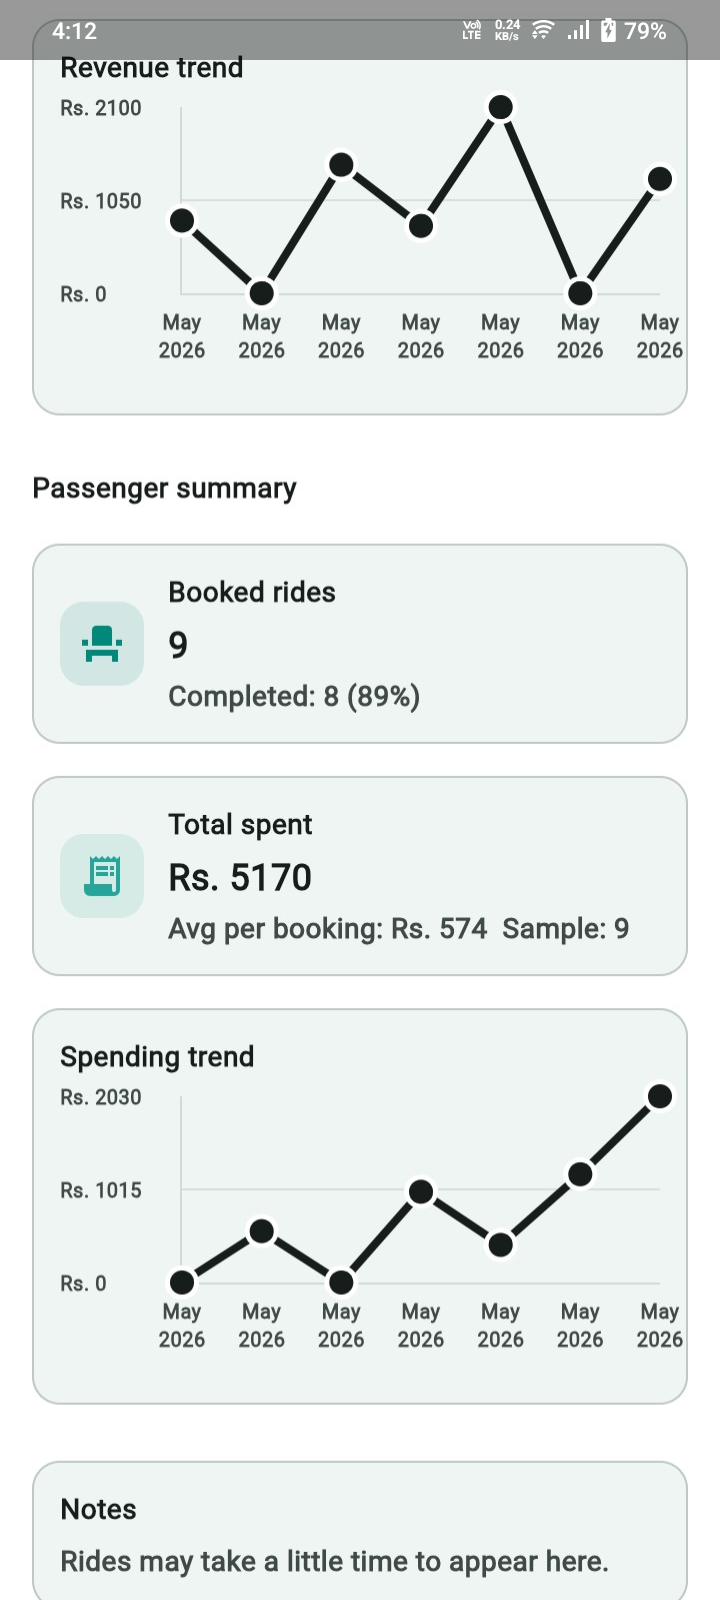
\includegraphics[width=\textwidth,height=0.6\textheight,keepaspectratio]{assets/app screenshot/analytics_part_2.jpeg}}
\end{minipage}
\caption{Profile Analytics}
\end{figure}

\subsubsection{Screen 38: Ride History (Booked/Created)}

Use for: Accessing and reviewing previous trip information.

\textbf{Components:}
\begin{itemize}
    \item History records with details of the routes.
\end{itemize}

\begin{figure}[H]
\centering
\begin{minipage}{0.45\textwidth}
\centering
\fbox{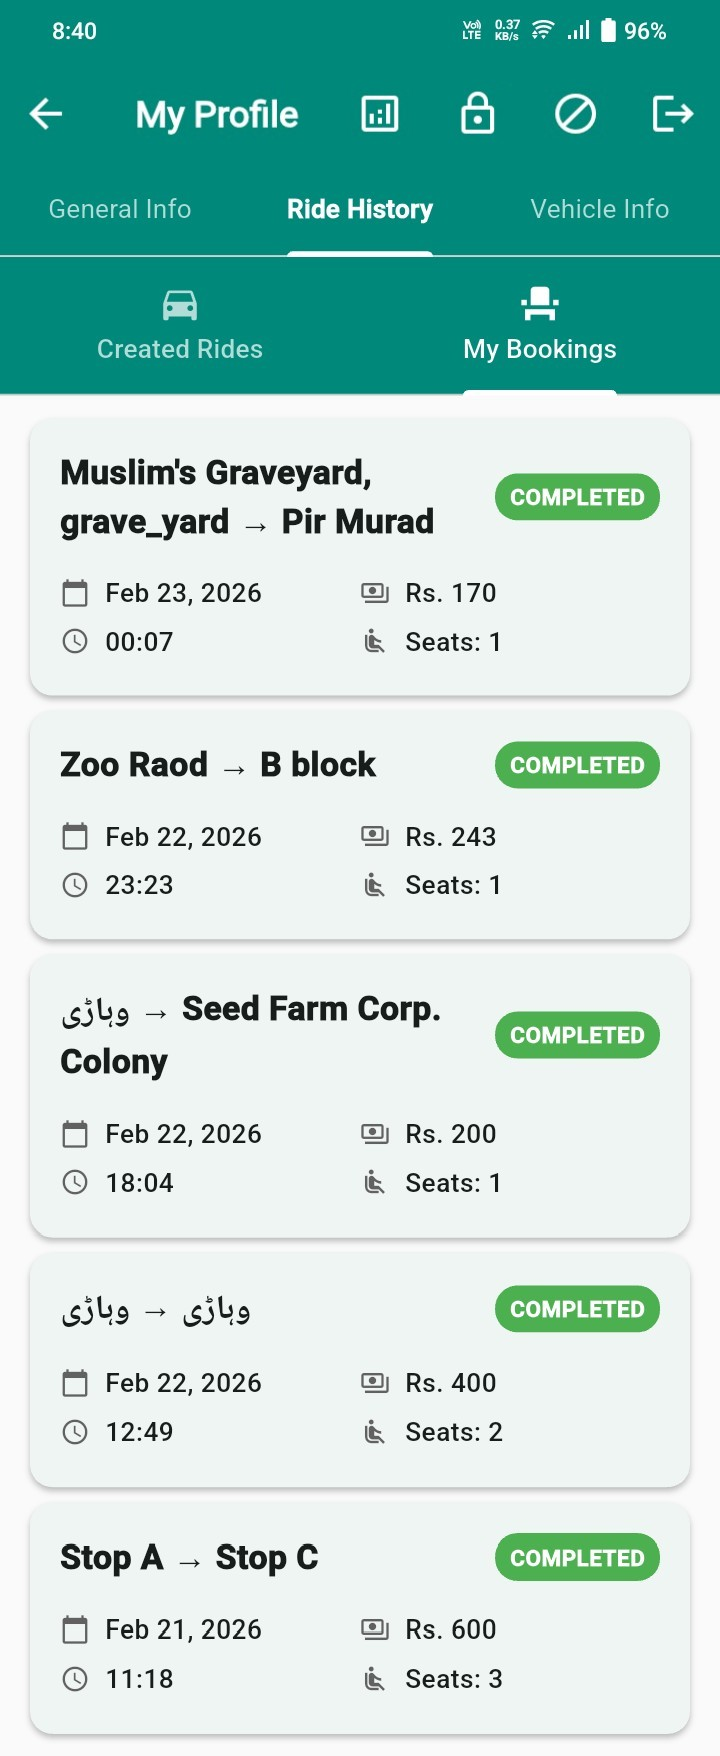
\includegraphics[width=\textwidth,keepaspectratio]{assets/app screenshot/profile_booked_ride_history.jpeg}}
\end{minipage}\hfill
\begin{minipage}{0.45\textwidth}
\centering
\fbox{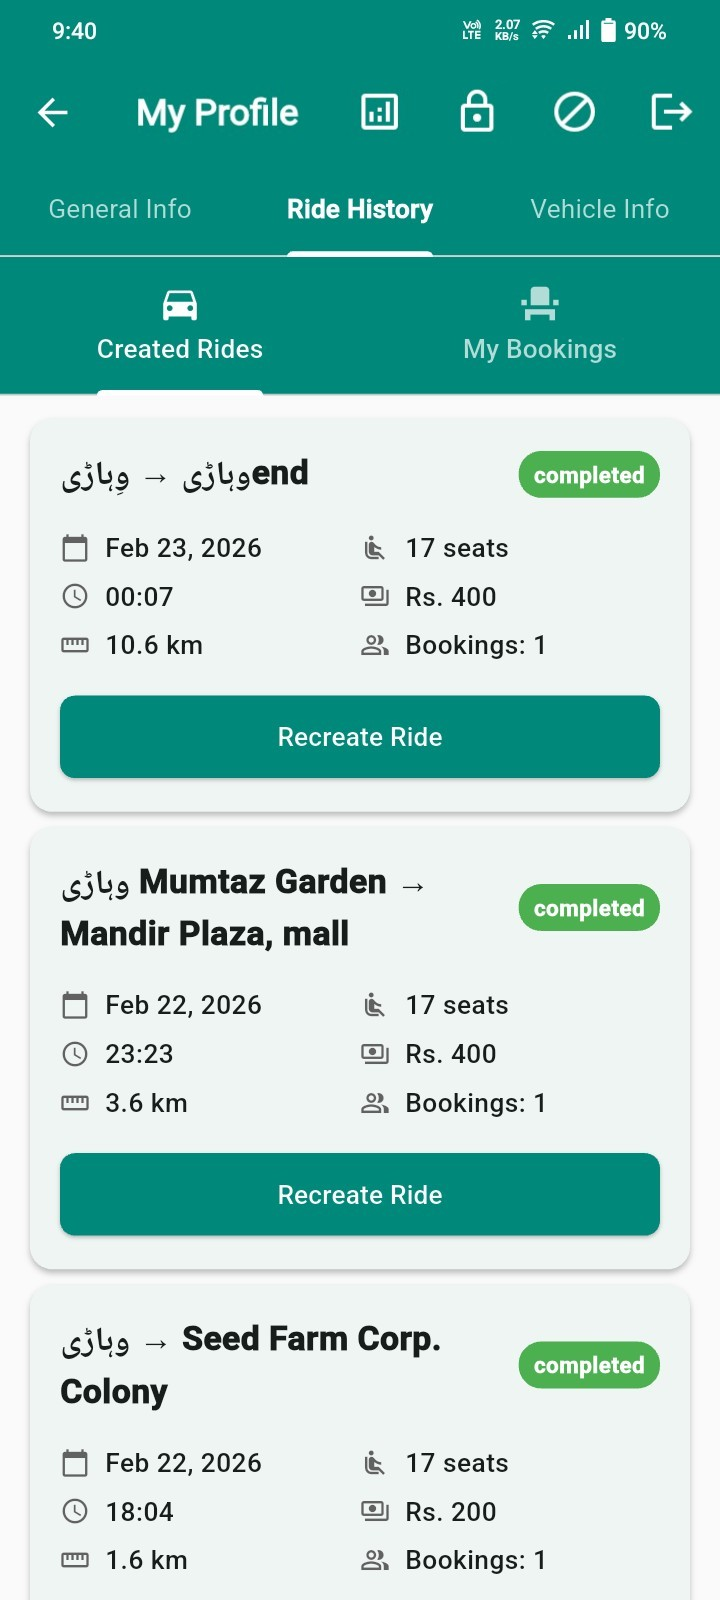
\includegraphics[width=\textwidth,keepaspectratio]{assets/app screenshot/profile_created_rides_history.jpeg}}
\end{minipage}
\caption{Ride History (Booked/Created)}
\end{figure}

Functional Flow: User scrolls through rides and views key ride information (route summary, status). Clicking on an item can trigger more detailed views, based on role and availability.

Backend integration: Ride history is loaded from booking/trip history endpoints, including pagination for large histories.

Validation/Security: Data from history is only accessible to the owner account and details of passengers/drivers is kept to a minimum in list views.

\subsubsection{Screen 39: Driver Verification Documents (Edit)}

Use this screen to edit the driver verification documents.This screen is used for editing the driver verification documents.

The purpose of this document is to provide a portal for keeping drivers and vehicles eligible.

\textbf{Components:}
Uploading images and inputting ID and vehicle registration.

\begin{figure}[H]
\centering
\begin{minipage}{0.30\textwidth}
\centering
\fbox{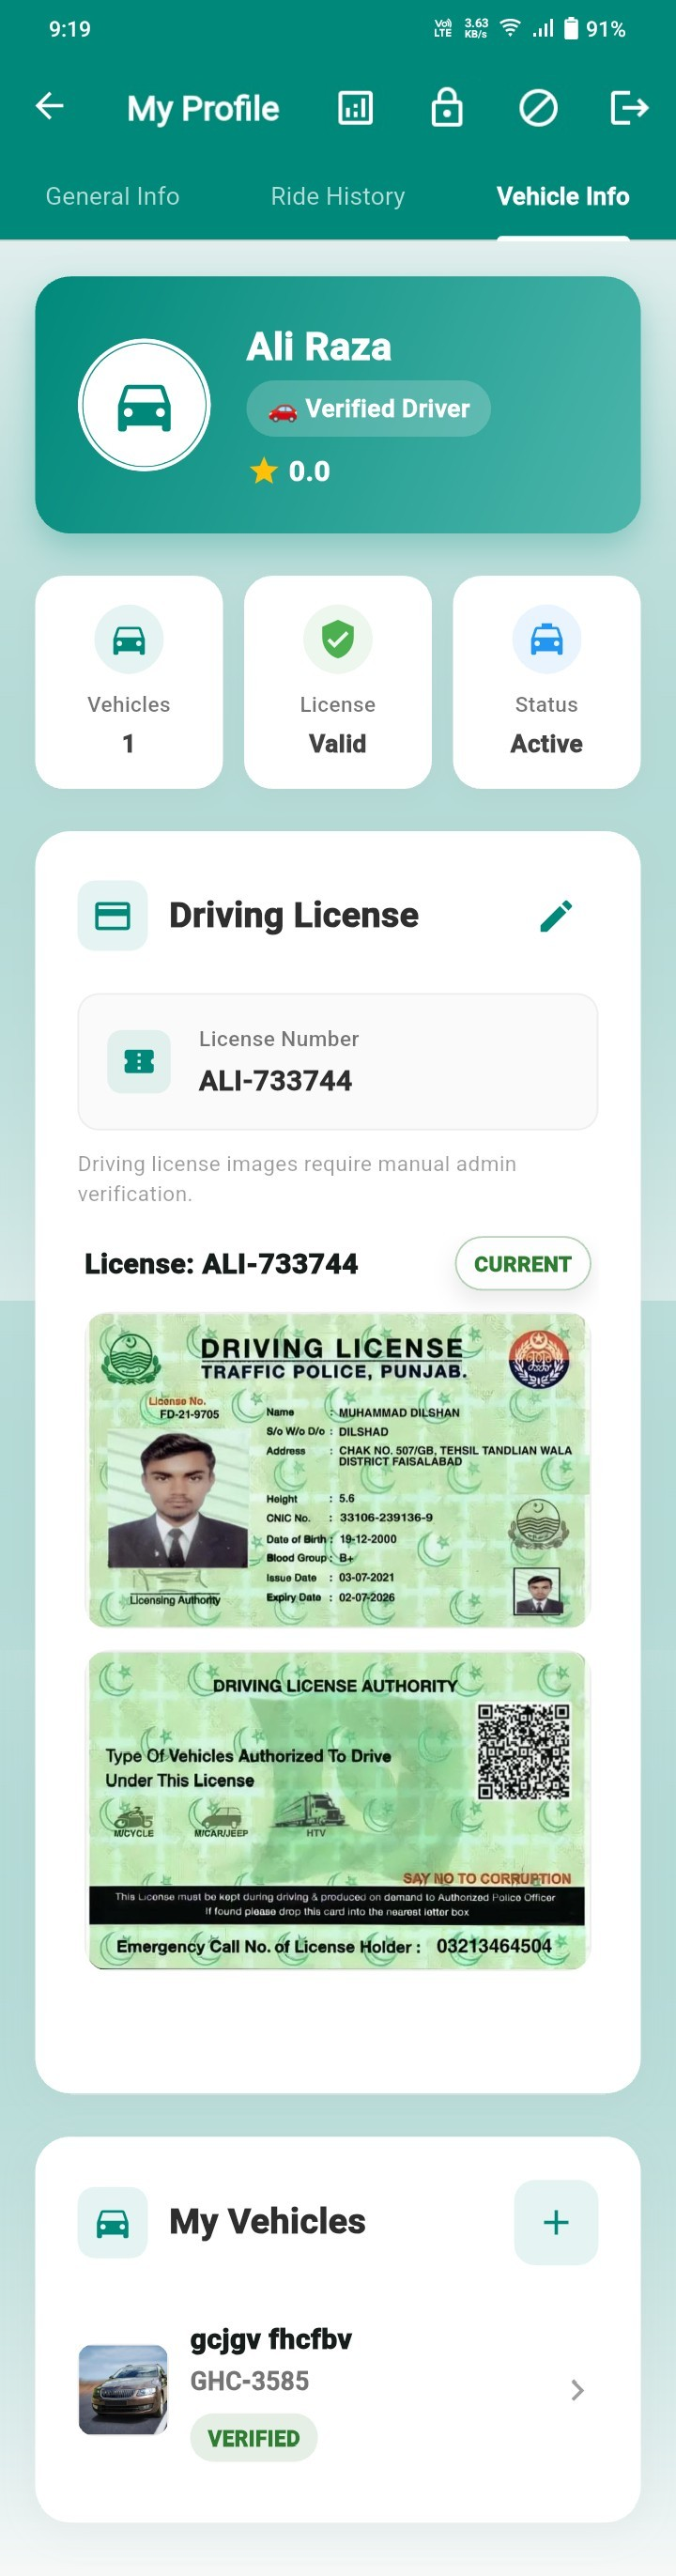
\includegraphics[width=\textwidth,height=0.55\textheight,keepaspectratio]{assets/app screenshot/driver_license_vehicle_info.jpeg}}
\end{minipage}\hfill
\begin{minipage}{0.30\textwidth}
\centering
\fbox{
\includegraphics[width=\textwidth,keepaspectratio]{assets/app screenshot/edit_driving_license.jpeg}}
\end{minipage}\hfill
\begin{minipage}{0.30\textwidth}
\centering
\fbox{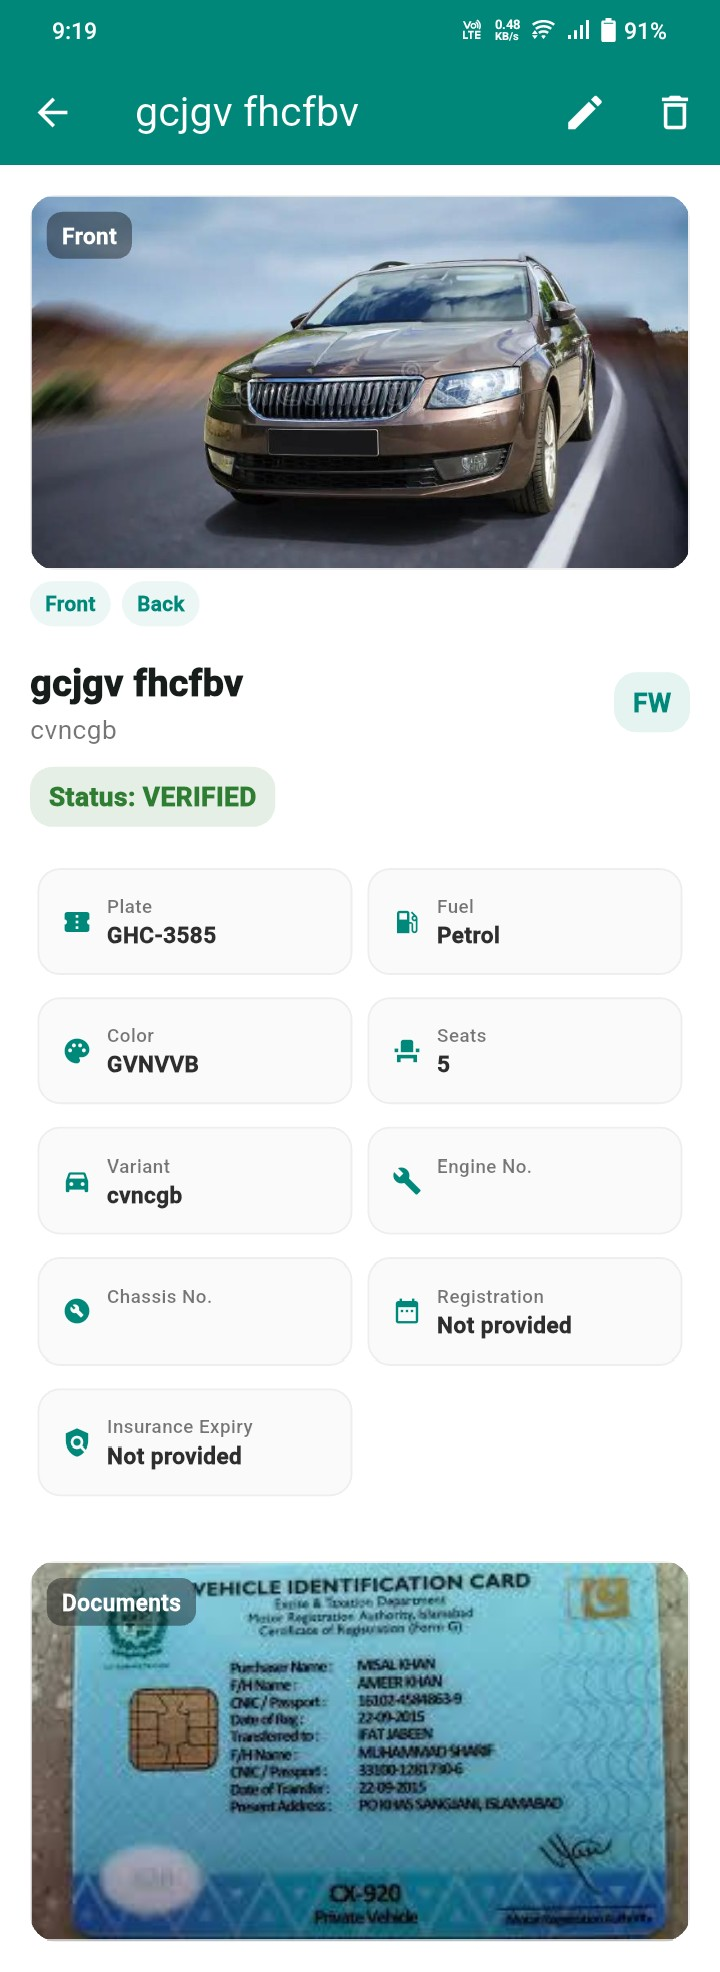
\includegraphics[width=\textwidth,keepaspectratio]{assets/app screenshot/vehicle_details_card.jpeg}}
\end{minipage}
\caption{Driver Verification Documents (Edit)}
\end{figure}

Functional Flow: Drivers upload and/or update their license and vehicle documents and submit them for verification. The UI gives instant feedback and driver eligibility is based on the verification status.

\textbf{Backend Integration:} Document metadata and images are uploaded to the backend storage layer, and are correlated with the driver profile for Admin review.

\textbf{Validation/Security:} File types and sizes are validated, uploads must be authenticated and documents are only accessible to authorised roles.

\subsubsection{Screen 40: Blocked Users}

Purpose: Users can use the blocked accounts functionality to limit their interactions on the platform.

\textbf{Components:}
\begin{itemize}
    \item Blocked user list and user search/filter controls.
\end{itemize}

\begin{figure}[H]
\centering
\fbox{
\includegraphics[width=\textwidth,height=0.6\textheight,keepaspectratio]{assets/app screenshot/blocked_users_list.jpeg}}
\caption{Blocked Users}
\end{figure}

Functional Flow: User will see blocked accounts and will be able to unblock users to re-enable interaction. After a block/unblock operation, the list will be updated immediately.

Backend Integration: Block/Unblock actions are saved through profile privacy endpoints and are synced with access to chat and/or search.

Validation/Security: Blocking is done on the server side to prevent unwanted contact in the messaging and booking flow.

\subsubsection{Screen 41: Web Live Tracking (External)}

Web Live Tracking (External): Screen 41

\textbf{Target:} A person with access to a desktop computer.\textbf{Goal:} Enable a person to track their ride using a desktop computer.

\textbf{Components:}
Real time map and trip status for the desktop.

\begin{figure}[H]
\centering
\fbox{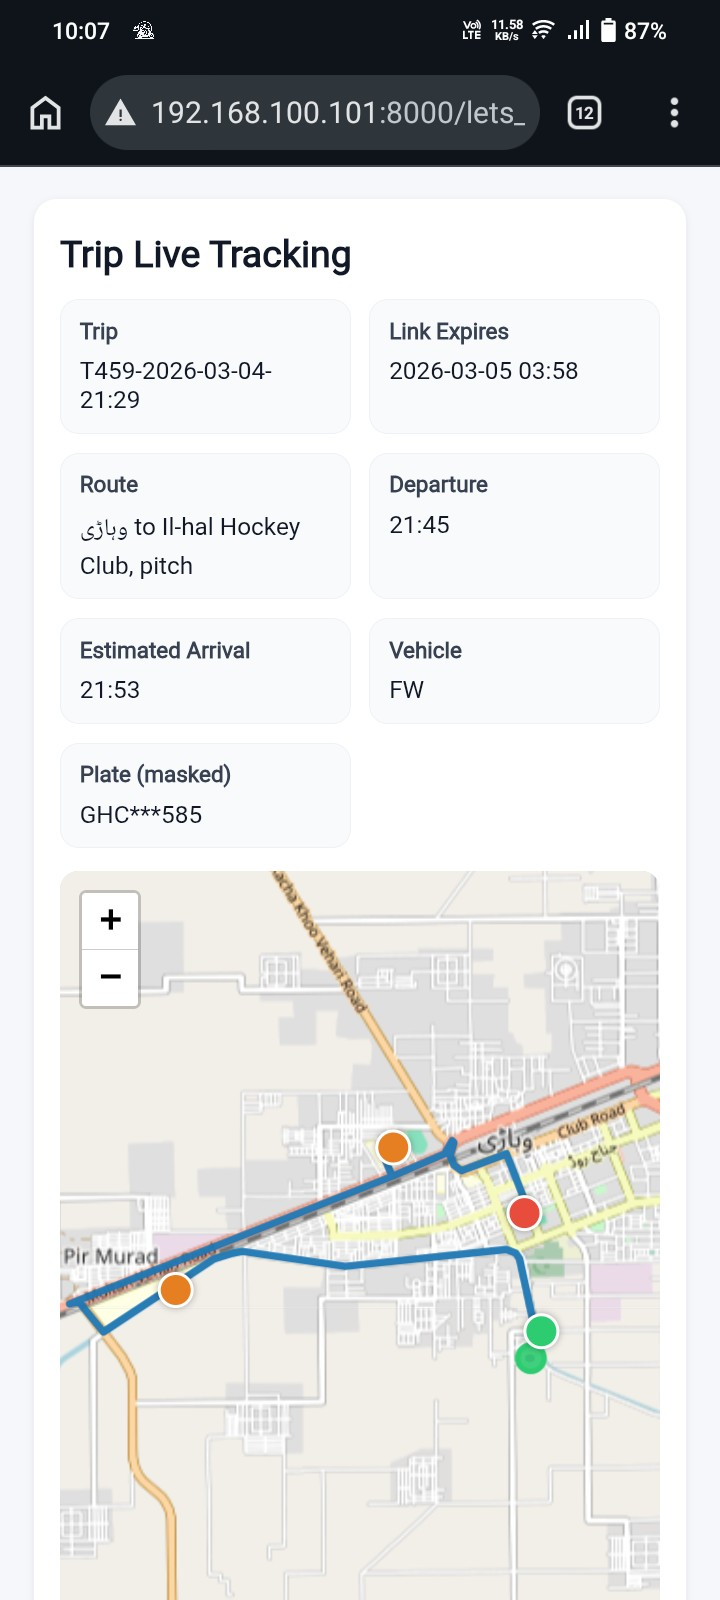
\includegraphics[width=\textwidth,keepaspectratio,height=0.6\textheight]{assets/app screenshot/web_live_tracking.jpeg}}
\caption{Web Live Tracking (External)}
\end{figure}

Functional Flow: The user accesses a web-based tracking view to see more of a trip on a larger screen. Active route and status are indicated on the map which is updated regularly.

Backend Integration: View subscribes to tracking endpoints for current location snapshots and tracking status changes.

Validation/Security: Data is shared only with authorised viewers (trip participants or Admin) and share links are validated before displaying data.

\textbf{Admin Module Overview:} Administrative web dashboards for monitoring rides, users, SOS incident, operational requests etc. are available in the administration module for authenticated users. Backend templates are used to serve all admin pages and role-based authorization is used to protect these pages.

\subsubsection{Screen 42: Admin Login}
Authorizes entry point for Admin authentication and session creation.

Components: Login form, error feedback and session/redirect handling.

Functional Flow: Admin provides credentials and receives authenticated session to access a protected dashboard.

Backend Integration: Administration login view and Session middleware.

\textbf{Validation/Security:} Server-side validation and access to dashboards is denied without a valid Admin session.

\begin{figure}[H]
\centering
\fbox{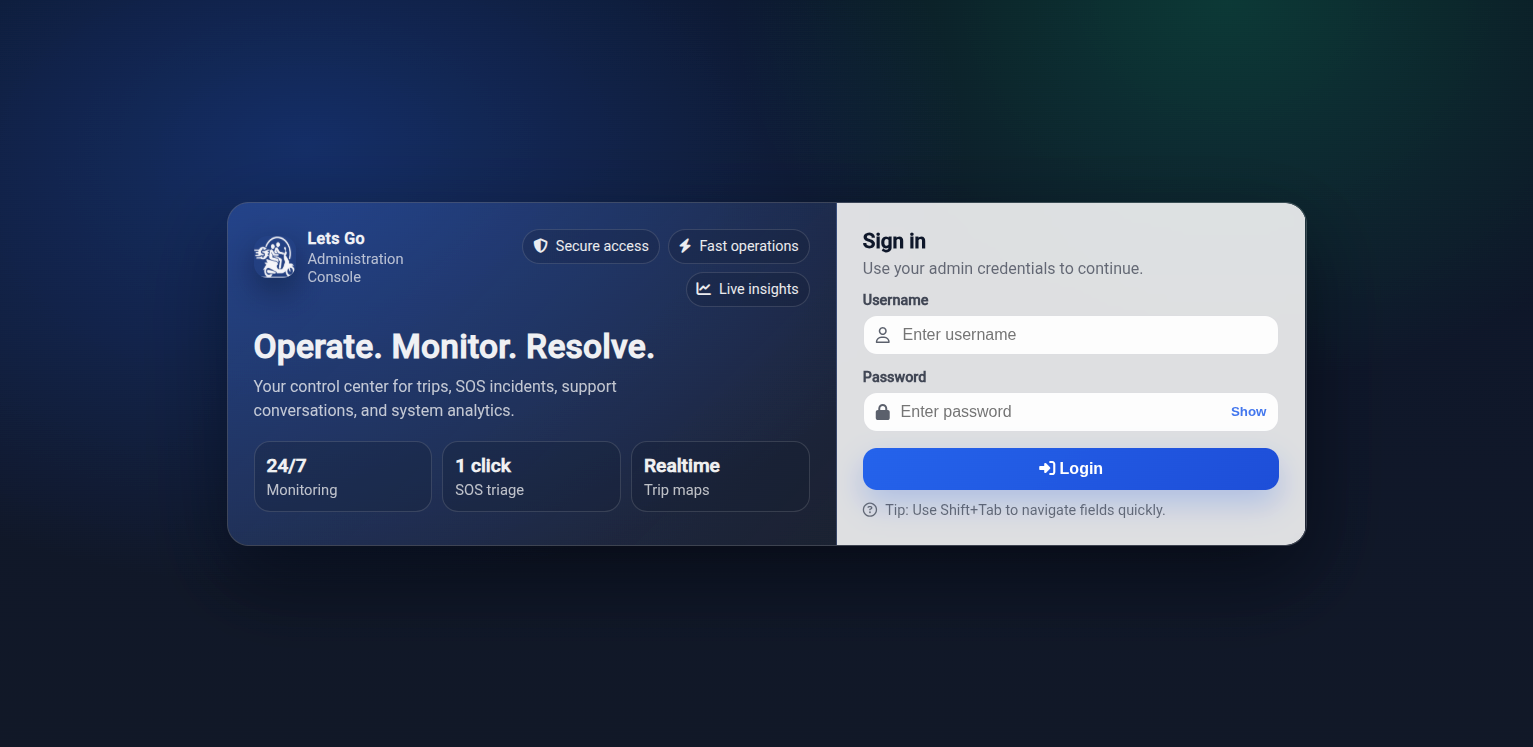
\includegraphics[width=0.85\textwidth,keepaspectratio]{assets/app screenshot/dashboard images/administration-login.png}}
\caption{Admin Login Screen}
\end{figure}

\subsubsection{Screen 43: Admin Dashboard (Overview)}
Purpose: High level view of platform health and important operational counters.

Components: Summary cards, quick links and key metric widgets.

Functional Flow: Fills summary cards and connects to more detailed dashboards like SOS and reached pending.

Backend Integration: Integrates ride, user and incident data from the administration dashboard view.

Validation/Security: Metrics are based on trusted data sources and displayed only to approved Admin roles.

\begin{figure}[H]
\centering
\fbox{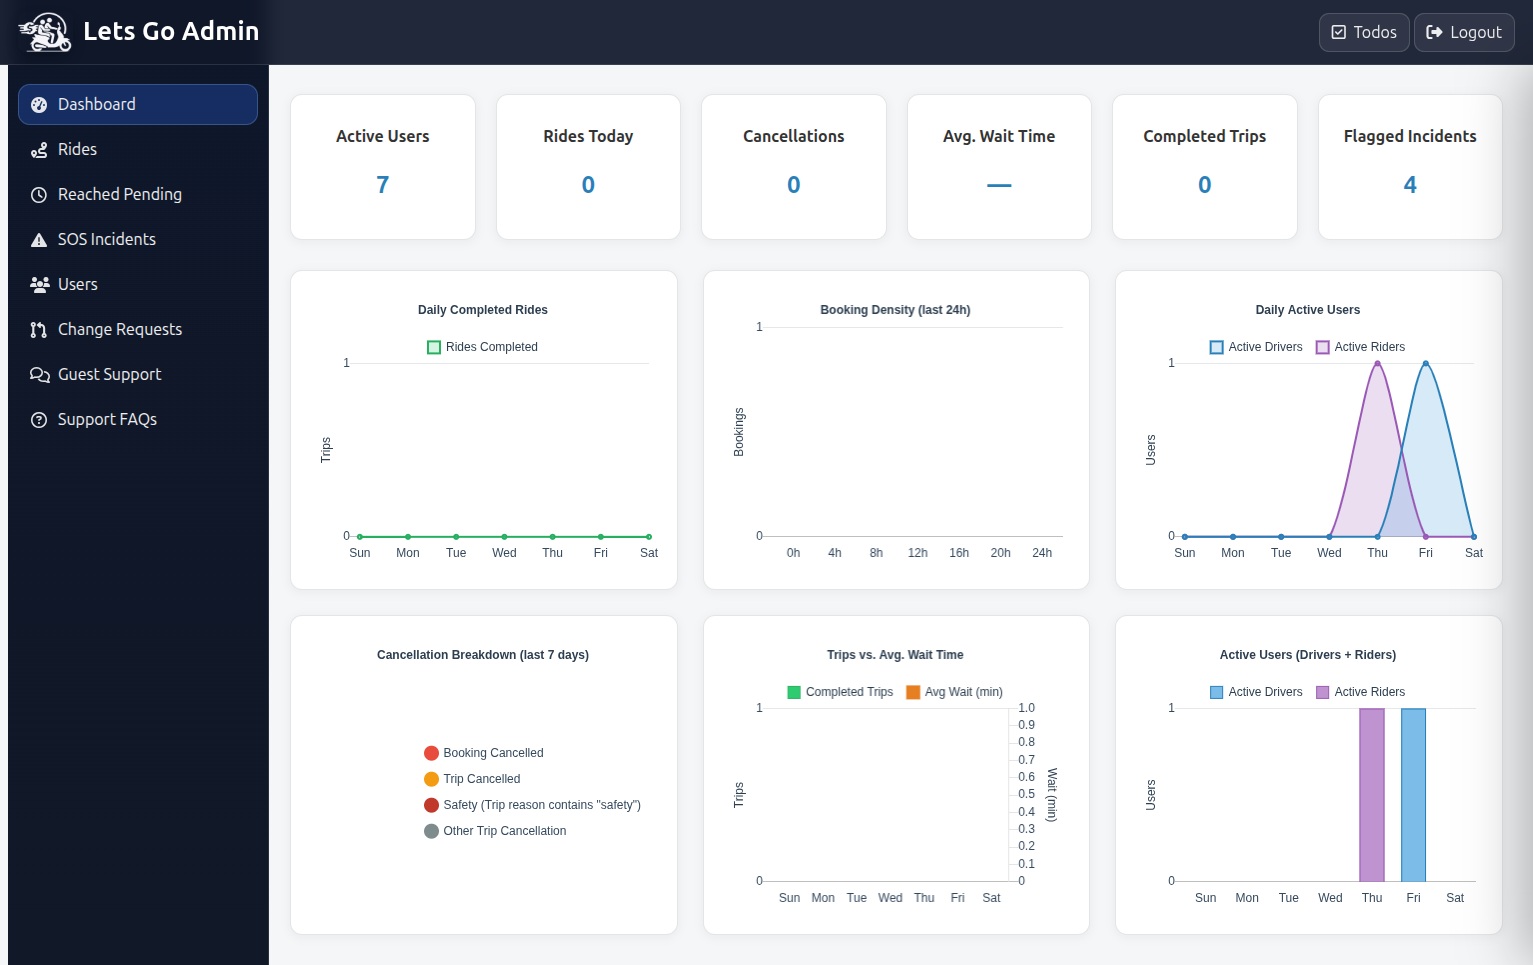
\includegraphics[width=0.85\textwidth,keepaspectratio]{assets/app screenshot/dashboard images/administration-dashboard.png}}
\caption{Admin Dashboard (Overview)}
\end{figure}

\subsubsection{Screen 44: Rides Dashboard}
\textbf{Description:} Watch published rides and ride lifecycle data.

Ride listing table, filters and navigation to ride/trip detail pages.

Functional Flow: Admin filters and views rides and opens trip detail pages to investigate rides.

Backend Integration: Provided through rides dashboard template and corresponding Django view.

Validation/Security: Only admin users have access to the admin area, and sensitive fields are not visible to non-admin users.

\begin{figure}[H]
\centering
\fbox{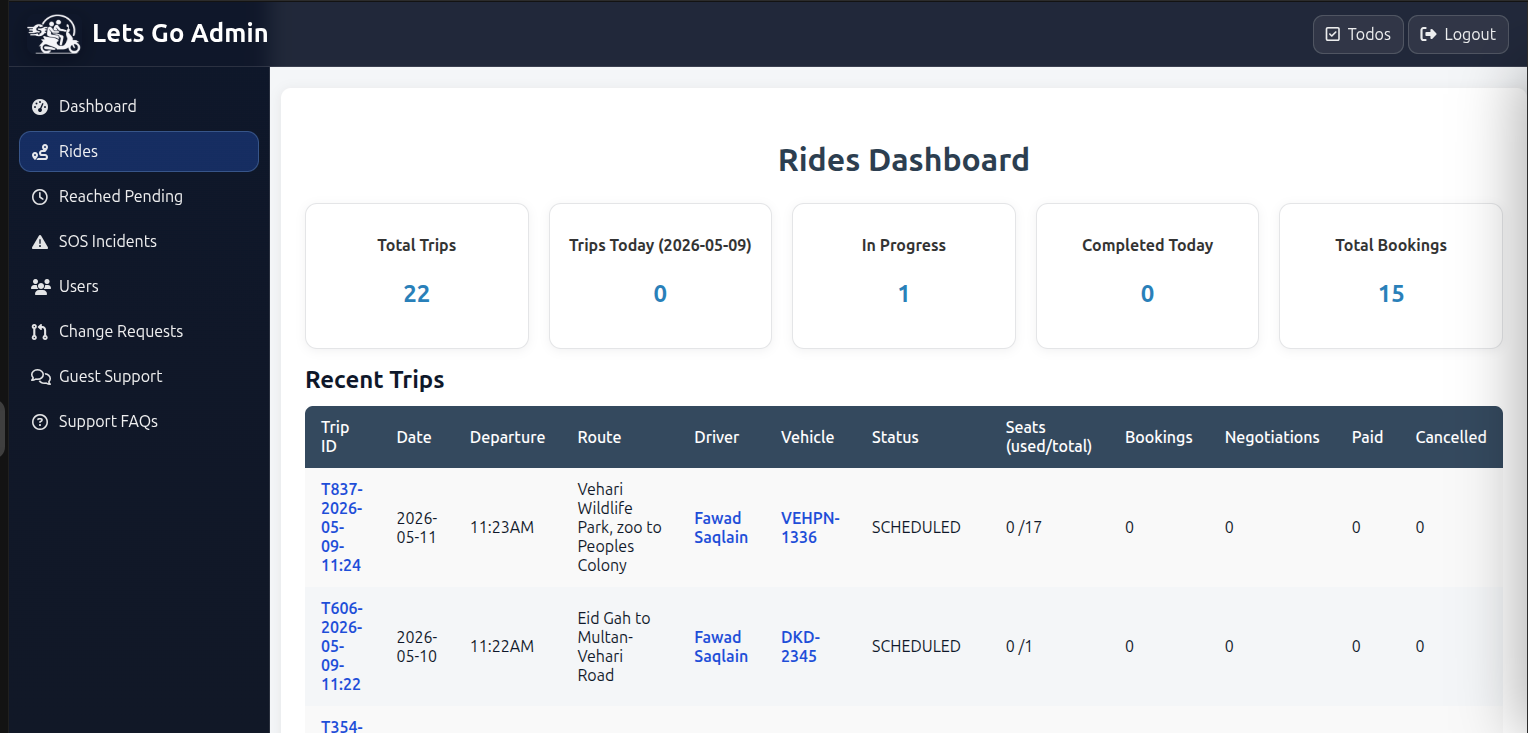
\includegraphics[width=0.85\textwidth,keepaspectratio]{assets/app screenshot/dashboard images/Rides-Dashboard.png}}
\caption{Rides Dashboard}
\end{figure}

\subsubsection{Screen 45: Reached Pending Dashboard}
Purpose: Identify riders who have reached/overdue status that needs follow-up.

The components are the pending/overdue list, status indicators and navigation controls.

Functional Flow: Admin reviews overdue entries and moves on to detail screens for action.

Backend Integration: With reached overdue dashboard view and template.

Validation/Security: List is created from verified ride states and only accessible in authenticated Admin sessions.

\begin{figure}[H]
\centering
\fbox{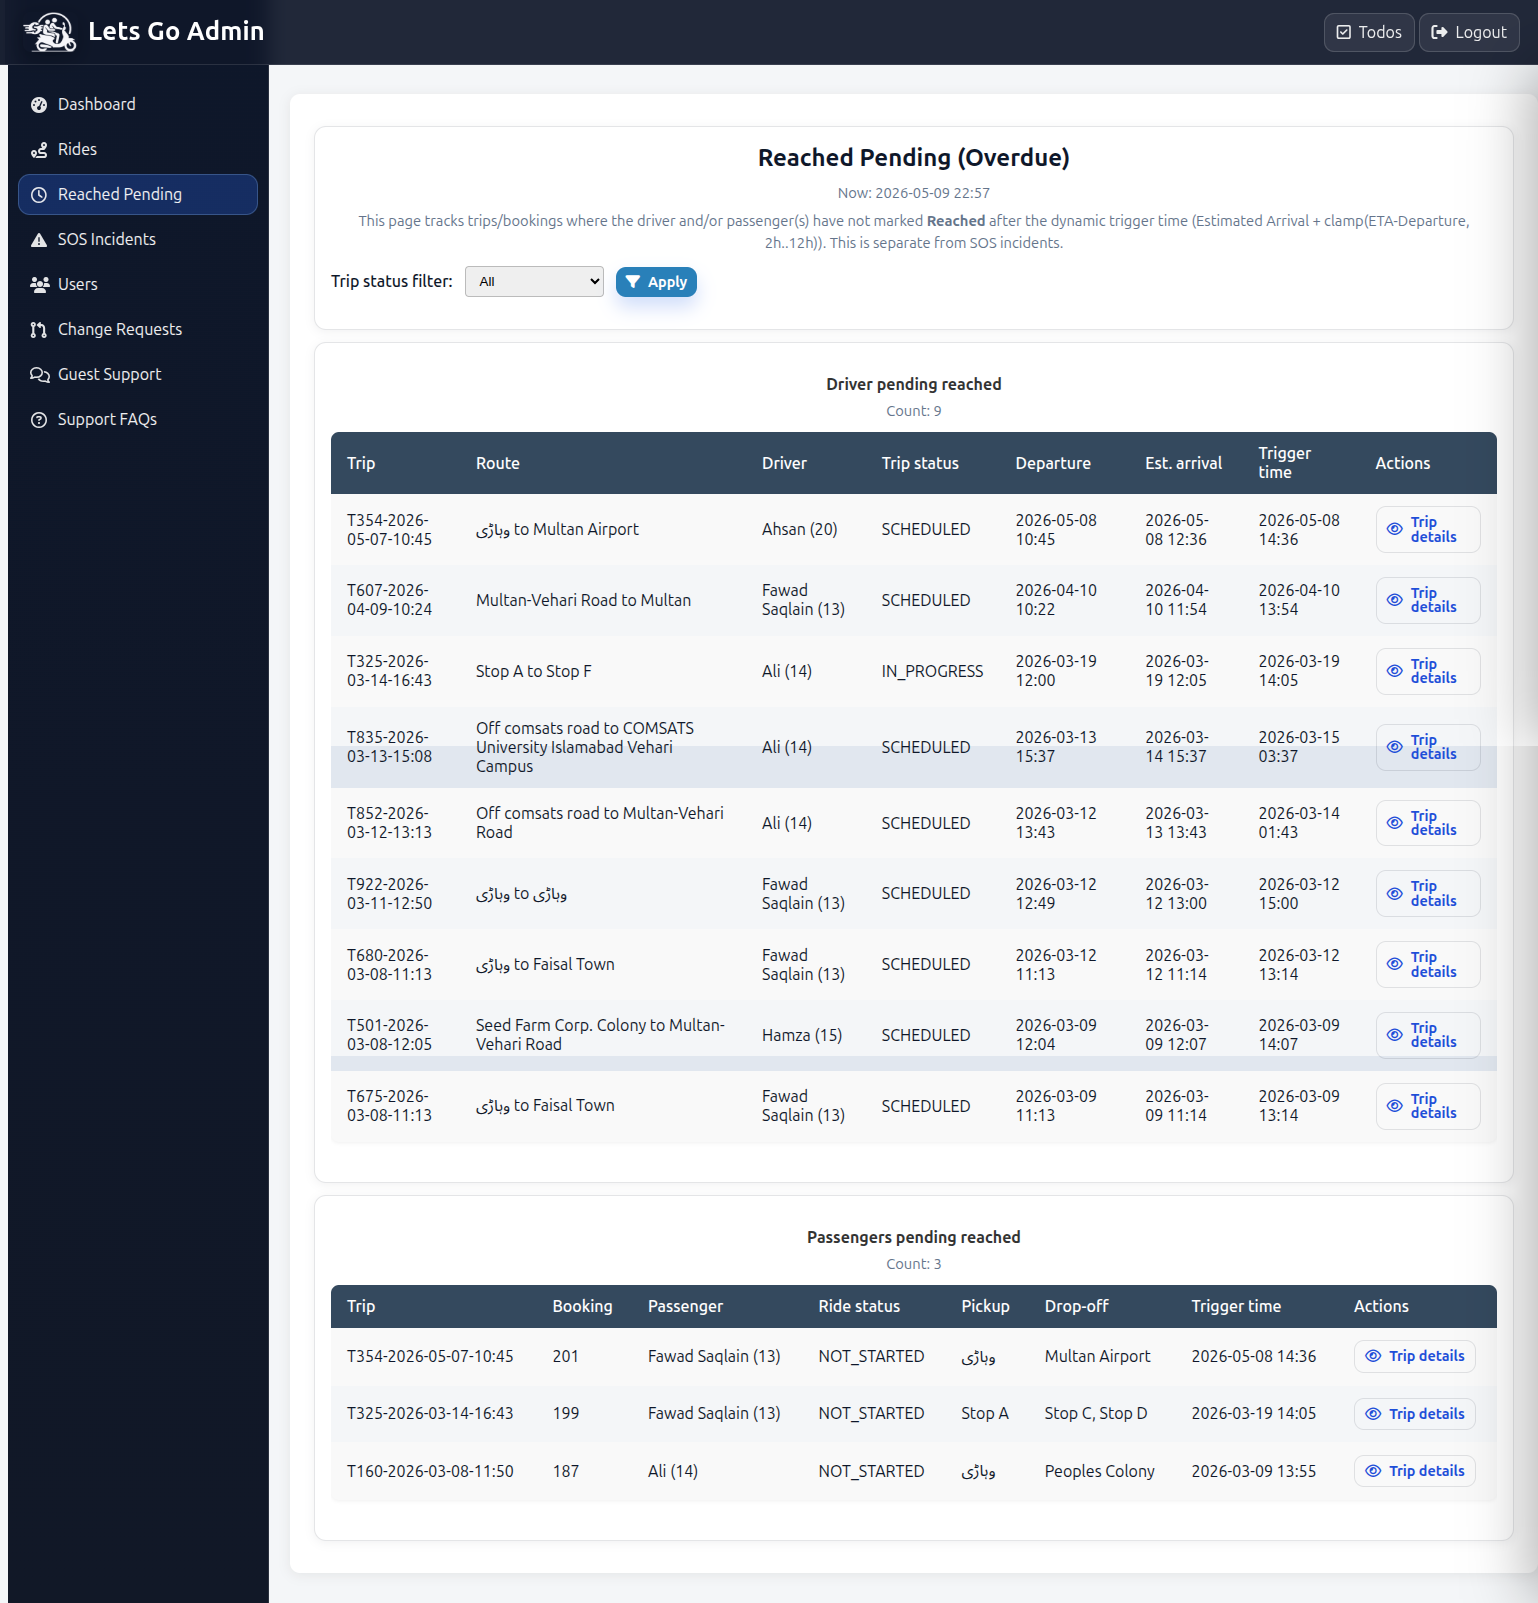
\includegraphics[width=0.85\textwidth,keepaspectratio]{assets/app screenshot/dashboard images/administration-reached.png}}
\caption{Reached Pending Dashboard}
\end{figure}

\subsubsection{Screen 46: SOS Incidents Dashboard}
Safety Monitoring Dashboard for reviewing, reacting to and resolving SOS incidents.

Components: Incident table, incident detail navigation, resolution/Status controls.

Admin opens an incident, reads through the location and metadata, and checks it off when action is taken.

Backend Integration: Backend dashboards and incident detail views served from Django templates.

Security/Validation: Access to incidents is role-restricted, and all state changes are done server side.

\begin{figure}[H]
\centering
\fbox{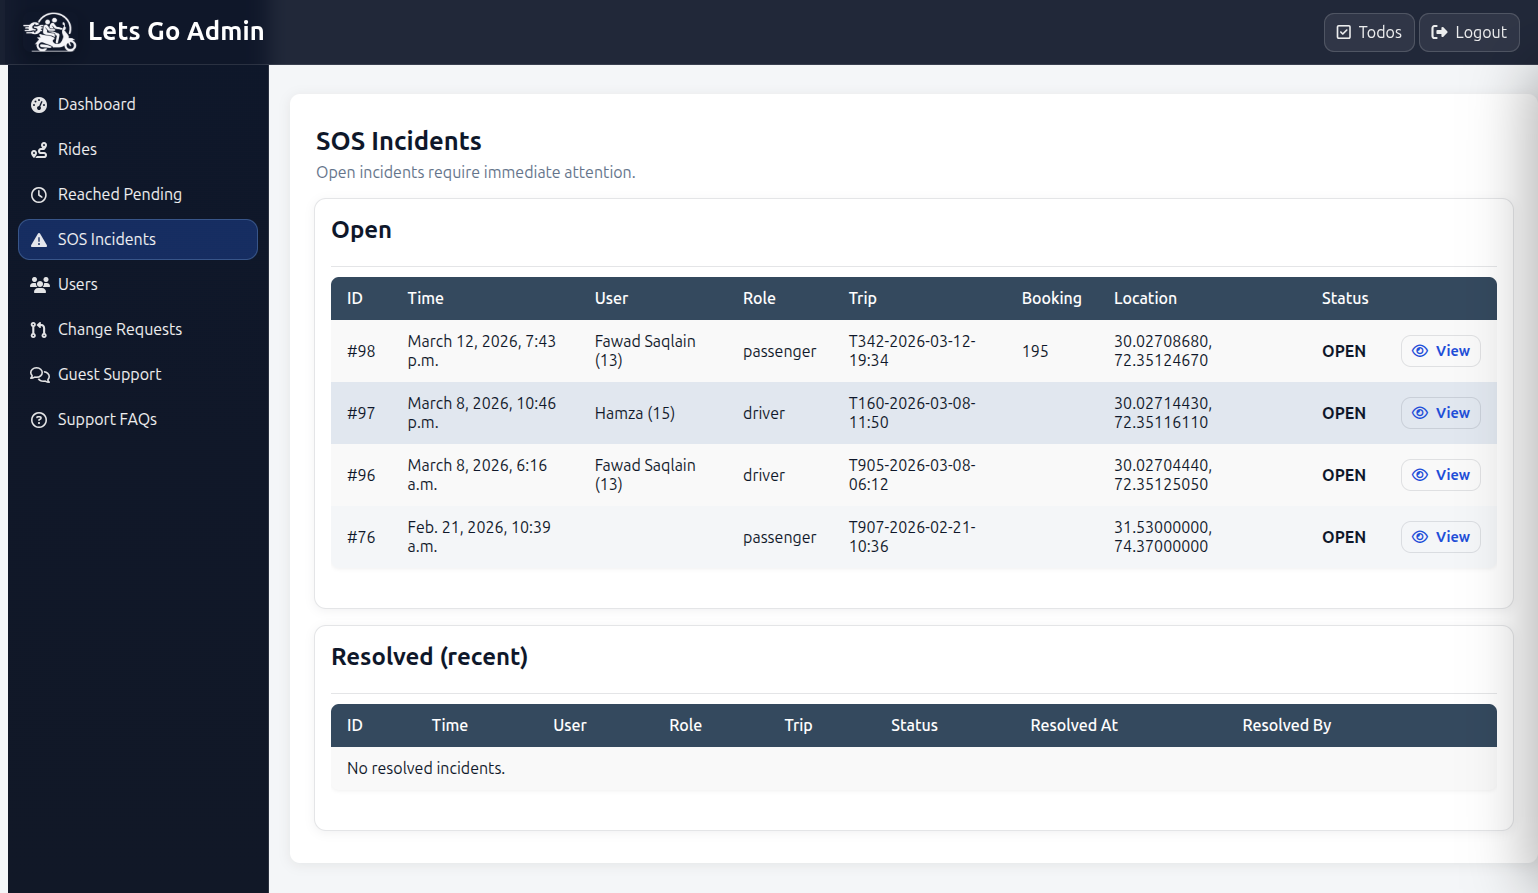
\includegraphics[width=0.85\textwidth,keepaspectratio]{assets/app screenshot/dashboard images/administration-sos.png}}
\caption{SOS Incidents Dashboard}
\end{figure}

\subsubsection{Screen 47: Users Management}
Purpose: to control the user accounts, to check the status, and to help with moderation processes.

Features include user list/search, detail views and administrative action controls.

Functional Flow: Admin searches users, opens details, and does allowed actions according to the policy.

Backend Integration: Loaded in User list/detail views in the admin module.

Validation/Security: Server-side validation of actions and only for Admin roles.

\begin{figure}[H]
\centering
\fbox{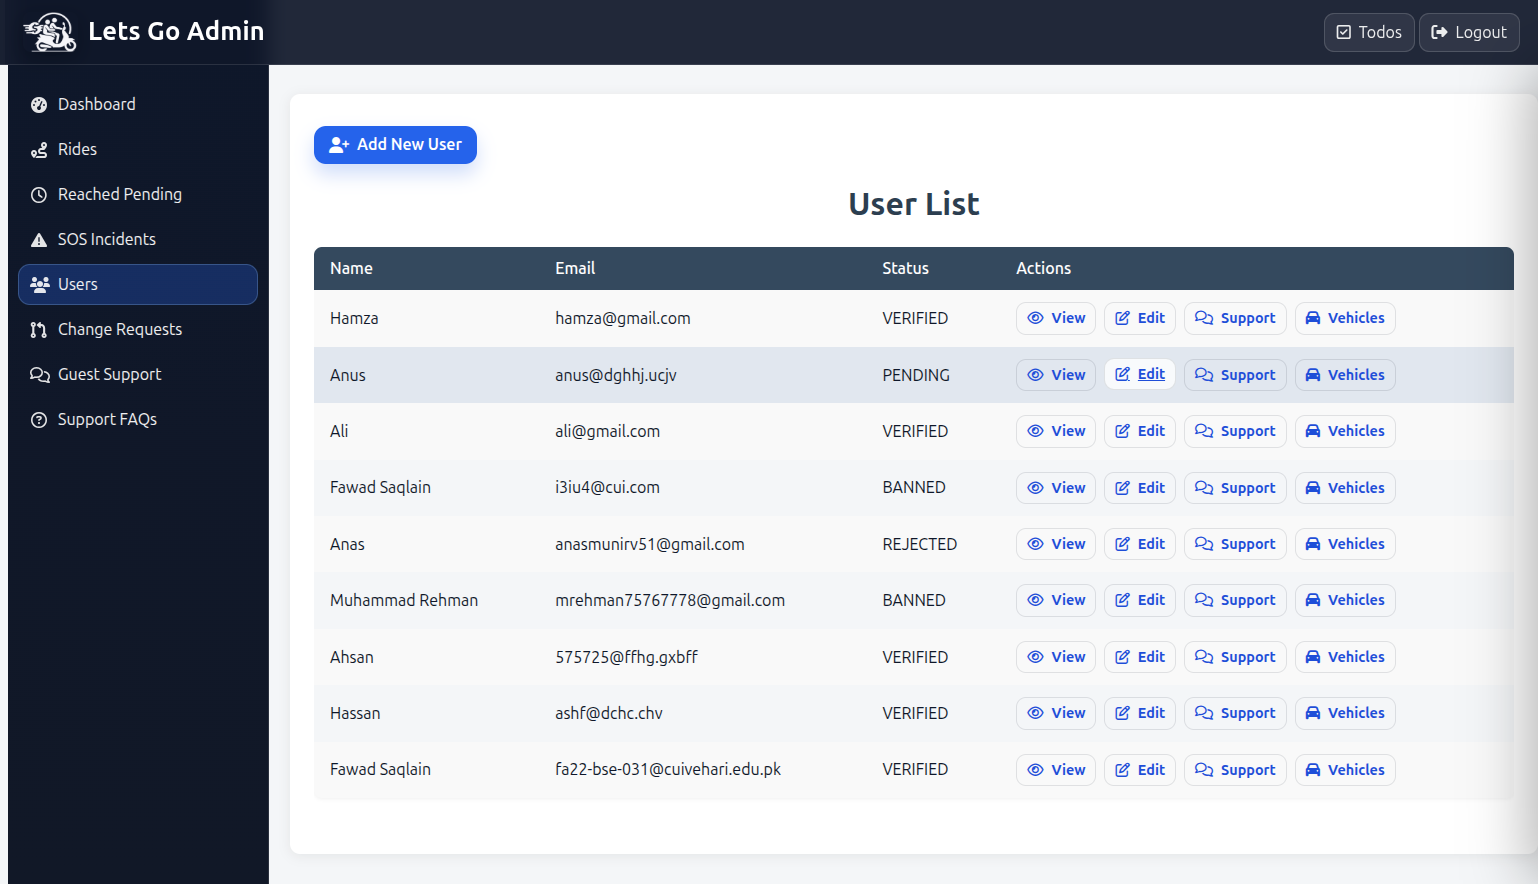
\includegraphics[width=0.85\textwidth,keepaspectratio]{assets/app screenshot/dashboard images/administration-users.png}}
\caption{Users Management Screen}
\end{figure}

\subsubsection{Screen 48: Change Requests Dashboard}
Use to monitor and log ride change requests from users.

The following components will be used: Request queue, request detail views, and approve and reject controls.

Functional Flow: Admin checks each request, and based on constraints he approves or rejects.

Backend Integration: Was provided through change request list/detail templates and views.

All requests are validated against ride constraints; any decisions are made server side (validation/security).

\begin{figure}[H]
\centering
\fbox{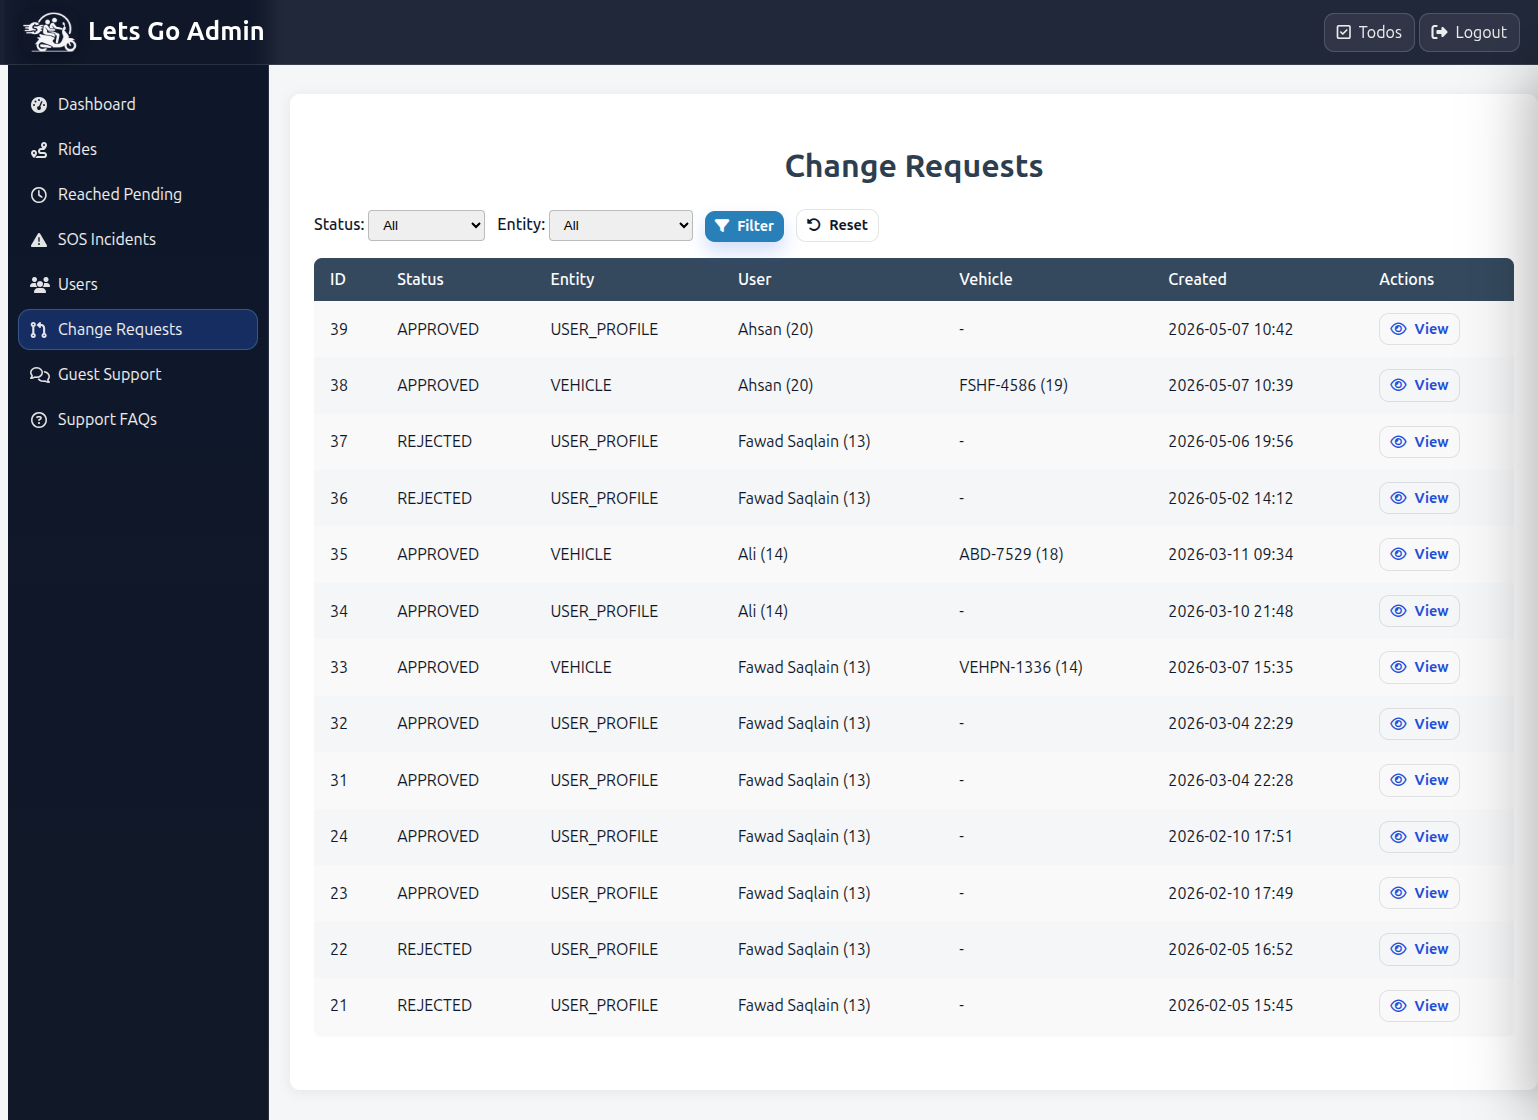
\includegraphics[width=0.85\textwidth,keepaspectratio]{assets/app screenshot/dashboard images/administration-change-requests.png}}
\caption{Change Requests Dashboard}
\end{figure}

\subsubsection{Screen 49: Admin Todos Inbox}
Purpose: Single source of information for tasks and follow-ups in operation.

Components: ToDo items and links to other entities, as well as task status indicators.

Functional Flow: Admin approves pending records and clicks on related entities to finish the job.

Back end integration: Embedded todos inbox view and supporting endpoints.

The following are also secured: Validation/Security: Todos can only be accessed by Admin sessions, updates to tasks are persisted using a secured endpoint.

\begin{figure}[H]
\centering
\fbox{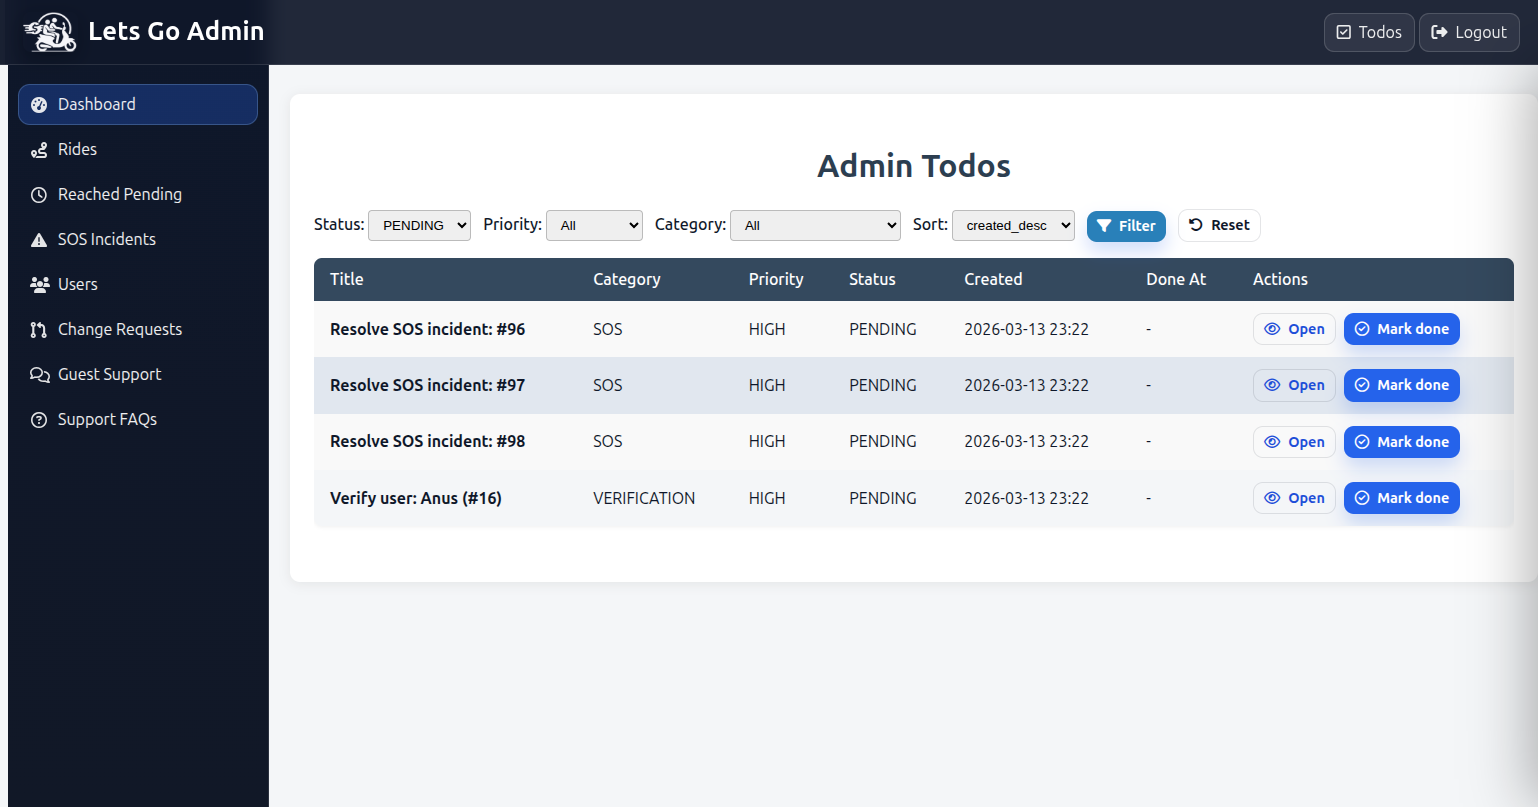
\includegraphics[width=0.85\textwidth,keepaspectratio]{assets/app screenshot/dashboard images/administration-todos.png}}
\caption{Admin Todos Inbox}
\end{figure}

\subsubsection{Screen 50: Support FAQs Management}
Purpose: Control FAQ entries for use by support and bot responses.

The components include the FAQ list, add/edit form, and the publish/update control.

Functional Flow: Admin adds / edits FAQs and these are made available to user support flows.

Backend Integration: Utilizes FAQ CRUD views backed by administration database models.

Validation/Security: Only Admins can edit FAQs and input is checked for validation before adding content.

\begin{figure}[H]
\centering
\fbox{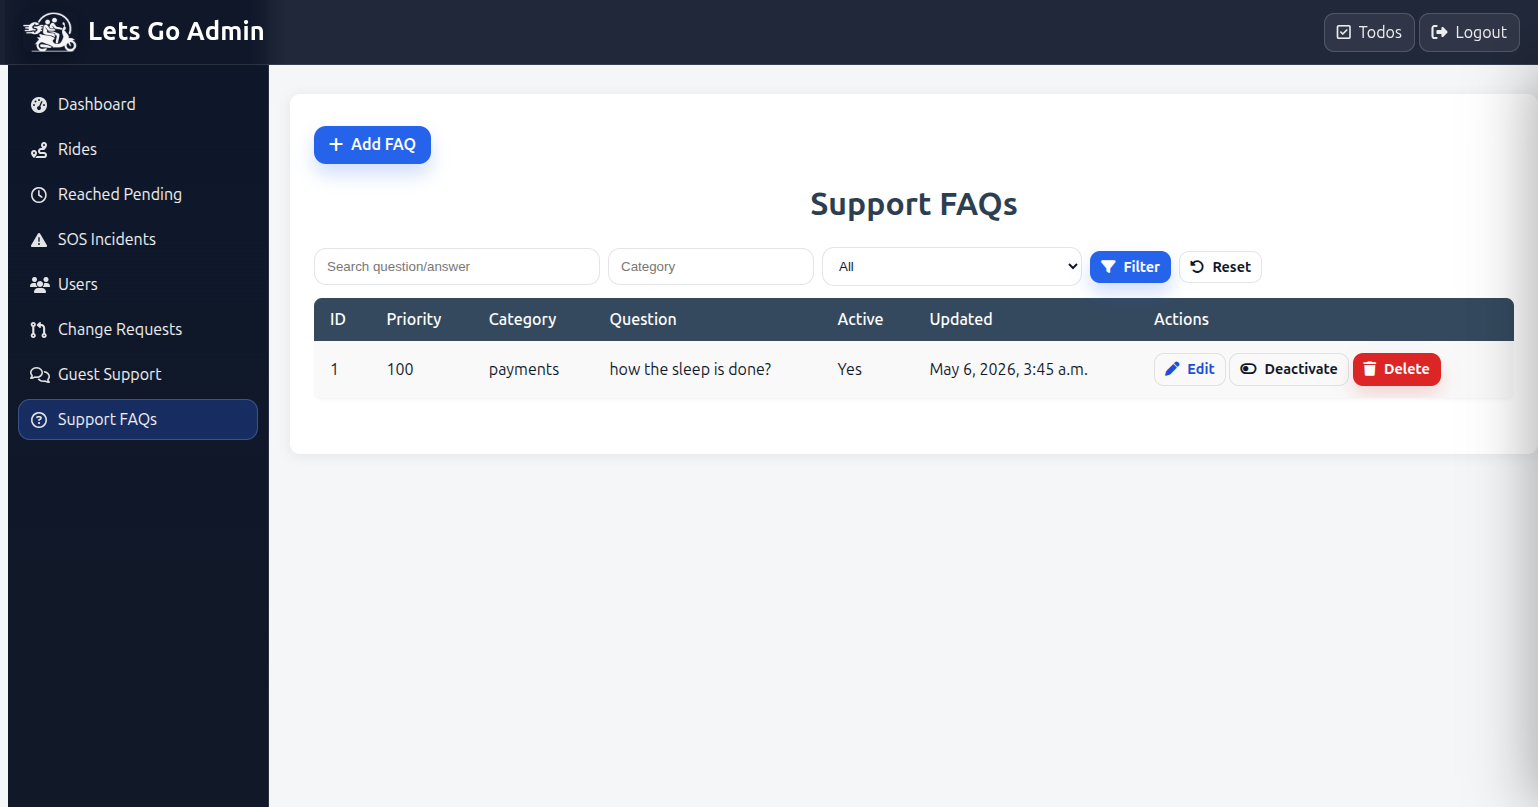
\includegraphics[width=0.85\textwidth,keepaspectratio]{assets/app screenshot/dashboard images/administration-support-faqs.png}}
\caption{Support FAQs Management}
\end{figure}

\subsubsection{Screen 51: Guest Support Users List}
The purpose of this is to be able to see the guests and to deal with support conversations without the need to have complete registration.

Components: Guest user list, access to chat thread, and support response tools.

Functional Flow: Admin is able to choose a guest user and then open the chat thread for resolution.

Guest List and chat templates are linked with the support message store, which powers Backend Integration.

Validation/Security: Guest threads are protected in accordance with the guest identity and only accessible for authorized admin sessions.

\begin{figure}[H]
\centering
\fbox{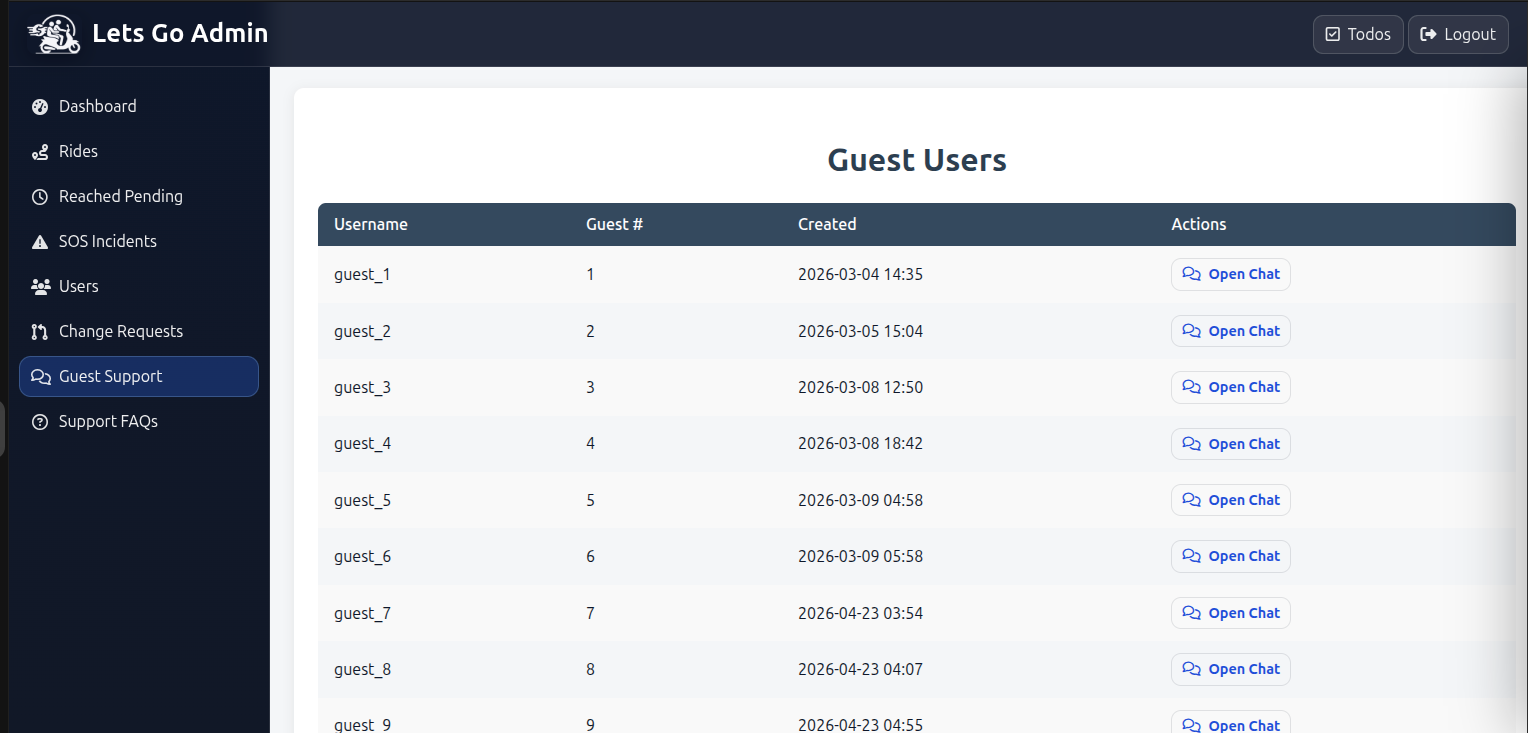
\includegraphics[width=0.85\textwidth,keepaspectratio]{assets/app screenshot/dashboard images/Guest-Users.png}}
\caption{Guest Support Users List}
\end{figure}

\subsection{Navigation Flow Diagram}

The route and the general navigation flow of the mobile app is shown below.

\begin{figure}[H]
\centering
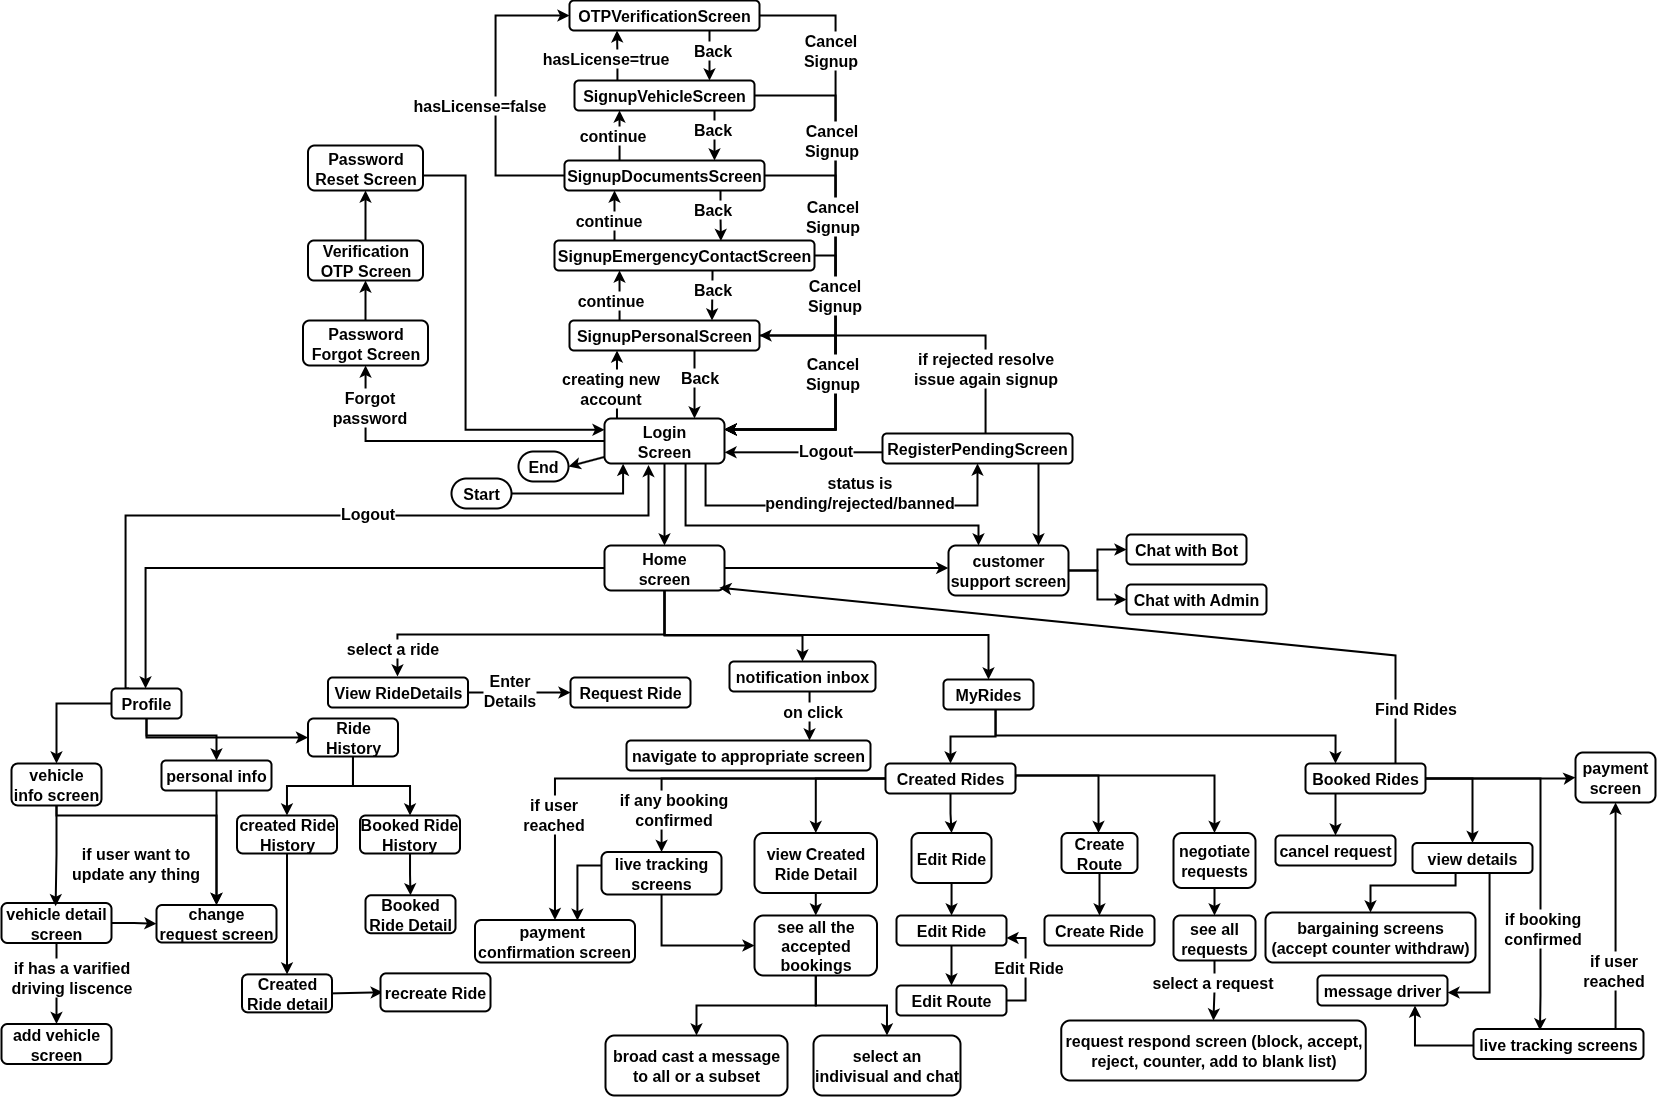
\includegraphics[width=0.9\textwidth,keepaspectratio,height=0.8\textheight]{assets/db_diagrams/navigation_flow_diagram.png}
\caption{Application Navigation Flow}
\end{figure}

\subsection{Responsiveness and Performance}

The Flutter app is made responsive to different screen sizes with the help of:

Wrapping layouts with -\texttt{LayoutBuilder} and -\texttt{MediaQuery} to adapt layouts.
- \texttt{Expanded} and \texttt{Flexible} widgets for dynamic spacing.
- Tabler layout for larger screens.

Performance considerations include:

- Long ride lists with pagination.
Document and media upload caching.
Efficient state updates to avoid unnecessary rebuilds.
Refreshed locations periodically rather than persistent socket connections.

% -------------------------------------------------
% 5.6 Deployment
% -------------------------------------------------

\section{Deployment}

The Django backend and Admin pages are deployed via cloud hosting and the database and file storage are managed via Supabase.

\begin{table}[htbp]
\centering
\caption{Deployment Details}
\begin{tabularx}{\textwidth}{|p{3cm}|p{3cm}|X|}
\hline
\textbf{Component} & \textbf{Platform} & \textbf{URL/Details} \\
\hline
Backend API & Vercel & Django backend deployment with function-based views and path-based routing \\
\hline
Database & Supabase & Managed PostgreSQL database used for application data \\
\hline
Admin Web Panel & Vercel & Django template-based Admin pages deployed with the backend \\
\hline
Mobile App (Android) & GitHub Releases & Direct APK distribution for testers and users \\
\hline
Storage & Supabase Storage & Object storage for user documents and media \\
\hline
\end{tabularx}
\end{table}

CI/CD: These are integrated with the hosting platform and run via GitHub Actions:

Backend \& Admin Pages: Automatically deploy changes to the hosting environment when they're merged to the \texttt{main} branch.
- Mobile App: Automated build pipelines to build release-ready APKs, uploaded to GitHub Releases.

\textbf{Security Measures:}

- HTTPS Encryption: TLS protects data that is being transferred.
- Authentication: authenticated user access via Django sessions.
Environment Security: Sensitive credentials and API keys are stored in environment variables and not hard-coded.

% -------------------------------------------------
% Chapter Summary
% -------------------------------------------------

\section*{Chapter Summary}

The chapter discussed the development environment, the core modules of the Lets Go Ride Sharing App system, the algorithms, external integrations and user interface implementation, and deployment of the Lets Go Ride Sharing App system. It is implemented in a modular fashion described in Chapter 4 and is implemented consistently using Django, Flutter, PostgreSQL on Supabase, and Supabase Storage.

Key achievements include:

- Documenting use cases and translating them to working code paths and back end workflows.
- Session based authentication and OTP based verification flows.
Ride creation, booking, negotiation, chat, tracking and SOS support.
Responsive mobile app that has screens that adapt to the screen being used and template-based Admin Pages.
Cloud deployment with Vercel, Supabase and GitHub Releases.

The system developed is now ready for a complete test and evaluation, which will be explored in the next chapter.

% ============================================
% Chapter 6 – Testing and Evaluation
% ============================================

\chapter{Testing and Evaluation}
\justifying

This chapter describes the testing strategies and evaluation procedures for verifying the correctness, reliability and performance of the Lets Go Ride Sharing App ride-sharing and recommendation system. Testing is used to verify the fulfillment of functional and non-functional requirements as described in previous chapters. The chapter includes unit testing, integration testing, system testing, performance testing, security testing, model evaluation (for the ML recommendation component), and finally, user acceptance testing.

% -------------------------------------------------
% 6.1 Testing Strategy
% -------------------------------------------------

\section{Testing Strategy}

Testing strategy for the Lets Go Ride Sharing App system is a multi-level strategy to test the system to ensure that it has been tested in a comprehensive manner throughout the development process. Manual testing and automated testing techniques were used.

Backend services were tested individually using \texttt{pytest}, and frontend components were tested using built-in Flutter test framework, for each unit and each function. External dependencies (such as database, APIs, etc.) were simulated using mock objects.

Using \texttt{Postman}, API interactions were tested for API endpoints and end-to-end testing of the Admin panel workflows were done manually. Database connectivity and integrity of transactions were checked.

All end-to-end workflows for each of the use cases (UC-1 to UC-25) were performed using manual and automated scripts. Edge cases, error handling and user journeys were checked.

Load testing was conducted using the \texttt{Apache JMeter} software, which was used to simulate a number of concurrent users and to test the response times, throughput, and resource utilization under load.

Security Testing: Security testing was performed using tools such as \texttt{OWASP ZAP} and manual penetration tests, including authentication mechanisms, role-based access control, input validation and data encryption.

Historical ride data was used to evaluate offline the content-based recommendation algorithm, using metrics like precision, recall and F1-score.

After testing the application, user feedback was gathered from a group of potential users (students and staff) to make necessary adjustments to the UI and usability issues.

Test cases and results were documented for all testing activities with the results compared with the expected results. Defects are managed and solved by defect tracking system (\texttt{GitHub Issues}).

% -------------------------------------------------
% 6.2 Unit Testing
% -------------------------------------------------

\section{Unit Testing}

Critical functions and classes were tested with unit tests both on the backend and frontend. Each test case is designed to test one unit of work using specific inputs, and to compare the outputs against a set of expected results. 480 were automated unit tests conducted.

\begin{table}[H]
\centering
\caption{Unit Testing Execution Summary}
\renewcommand{\arraystretch}{1.3}
\begin{tabularx}{\textwidth}{|l|X|c|c|c|c|}
\hline
\textbf{Section} & \textbf{Test Suite} & \textbf{Total} & \textbf{Passed} & \textbf{Failed} & \textbf{Pass \%} \\
\hline
A & Flutter Behavioral & 18 & 18 & 0 & 100\% \\
\hline
B & Flutter Contracts (Utils) & 45 & 45 & 0 & 100\% \\
\hline
B & Flutter Contracts (Controllers) & 59 & 59 & 0 & 100\% \\
\hline
B & Flutter Contracts (Screens) & 159 & 159 & 0 & 100\% \\
\hline
C & Backend Pytest & 199 & 199 & 0 & 100\% \\
\hline
\rowcolor{gray!15} \textbf{Total} & \textbf{All Suites} & \textbf{480} & \textbf{480} & \textbf{0} & \textbf{100\%} \\
\hline
\end{tabularx}
\end{table}

\subsection{Backend Unit Testing (Pytest)}

The \texttt{pytest} framework is used for the back-end test suite, which checks the logic of authentication, the posting of rides, and administration.

\begin{table}[H]
\centering
\caption{Backend – Authentication and Profile Views}
\renewcommand{\arraystretch}{1.3}
\begin{tabularx}{\textwidth}{|c|X|X|c|}
\hline
\textbf{ID} & \textbf{Unit Under Test} & \textbf{Expected Output} & \textbf{Result} \\
\hline
BT-01 & \texttt{\_parse\_json\_body} & Returns dict for valid JSON, else empty & Pass \\
\hline
BT-02 & \texttt{\_normalize\_gender} & Consistent lowercase mapping ("male"/"female") & Pass \\
\hline
BT-03 & \texttt{generate\_otp} & 8-digit numeric string for verification & Pass \\
\hline
BT-04 & \texttt{login} endpoint & 200 OK with session-based authentication and user profile & Pass \\
\hline
BT-05 & \texttt{check\_username} & Availability flag set according to registry & Pass \\
\hline
BT-06 & \texttt{send\_otp} & OTP dispatched and stored in cache & Pass \\
\hline
BT-07 & \texttt{verify\_otp} & Cache updated with \texttt{email\_verified=True} and/or \texttt{phone\_verified=True} & Pass \\
\hline
BT-08 & \texttt{upload\_to\_supabase} & Returns public URL after mock bucket upload & Pass \\
\hline
\end{tabularx}
\end{table}

\begin{table}[H]
\centering
\caption{Backend – Database Integration and Smoke Tests}
\renewcommand{\arraystretch}{1.3}
\begin{tabularx}{\textwidth}{|c|X|X|c|}
\hline
\textbf{ID} & \textbf{Unit Under Test} & \textbf{Expected Output} & \textbf{Result} \\
\hline
BT-09 & \texttt{Django Model Smoke} & CRUD operations on Users, Trips, and Bookings & Pass \\
\hline
BT-10 & \texttt{Booking.full\_clean} & Rejects bookings if from\_stop is after to\_stop & Pass \\
\hline
BT-11 & \texttt{\_decode\_ors\_polyline} & Converts encoded strings to coordinate lists & Pass \\
\hline
BT-12 & \texttt{update\_route\_geometry} & Bulk creates geometry points for planned paths & Pass \\
\hline
\end{tabularx}
\end{table}

\begin{table}[H]
\centering
\caption{Backend – Ride Posting and Trip Management}
\renewcommand{\arraystretch}{1.3}
\begin{tabularx}{\textwidth}{|c|X|X|c|}
\hline
\textbf{ID} & \textbf{Unit Under Test} & \textbf{Expected Output} & \textbf{Result} \\
\hline
BT-13 & \texttt{\_is\_archived\_after\_24h} & True if trip completed more than 24h ago & Pass \\
\hline
BT-14 & \texttt{create\_trip} (Illegal) & Returns 405 for GET requests & Pass \\
\hline
BT-15 & \texttt{\_calculate\_distance} & Haversine distance matches expected KM & Pass \\
\hline
BT-16 & \texttt{can\_cancel\_trip} & Boolean guard based on trip timing and status & Pass \\
\hline
BT-17 & \texttt{auto\_archive\_global} & Archives eligible trips up to configured limit & Pass \\
\hline
\end{tabularx}
\end{table}

\begin{table}[H]
\centering
\caption{Backend – Administration and SOS Handling}
\renewcommand{\arraystretch}{1.3}
\begin{tabularx}{\textwidth}{|c|X|X|c|}
\hline
\textbf{ID} & \textbf{Unit Under Test} & \textbf{Expected Output} & \textbf{Result} \\
\hline
BT-18 & \texttt{\_build\_sos\_snippet} & JSON snapshot includes incident and trip data & Pass \\
\hline
BT-19 & \texttt{\_attach\_latest\_payments} & Payment receipts linked to booking objects & Pass \\
\hline
BT-20 & \texttt{guest\_list\_view} & Renders admin guest management template & Pass \\
\hline
BT-21 & \texttt{vehicle\_update\_status} & Guards prevent illegal status transitions & Pass \\
\hline
BT-22 & \texttt{sos\_incident} logic & Atomic save of incident with coordination data & Pass \\
\hline
\end{tabularx}
\end{table}

\subsection{Frontend Behavioral Testing (Flutter)}

Behavioral tests are used to test the business logic and state management of the Flutter controllers.

\begin{table}[H]
\centering
\caption{Frontend – Routing and Path Execution Logic}
\renewcommand{\arraystretch}{1.3}
\begin{tabularx}{\textwidth}{|c|X|X|c|}
\hline
\textbf{ID} & \textbf{Unit Under Test} & \textbf{Expected Output} & \textbf{Result} \\
\hline
FT-01 & \texttt{validateActualPath} & True if stops are within threshold of actual path & Pass \\
\hline
FT-02 & \texttt{appendOnlyRule} & Rejects extension if previous stops are deleted & Pass \\
\hline
FT-03 & \texttt{loadExistingRouteData} & Controller fields match provided planned metadata & Pass \\
\hline
FT-04 & \texttt{ActualPathOverlay} UI & Toggle visibility based on overlay presence & Pass \\
\hline
FT-05 & \texttt{parseActualPath} & Complex JSON coordinates parsed into LatLng list & Pass \\
\hline
FT-06 & \texttt{applyRouteData} & Preserves overlay when route editor returns & Pass \\
\hline
\end{tabularx}
\end{table}

\subsection{Frontend Code Contract Verification}

Contract tests guarantees that all vital utility classes, controllers, and screens have the desired API surface and structure.

\begin{table}[H]
\centering
\caption{Frontend – Utilities and Controllers Contract Verification}
\renewcommand{\arraystretch}{1.3}
\begin{tabularx}{\textwidth}{|l|X|X|c|}
\hline
\textbf{Target Area} & \textbf{Symbol Verification} & \textbf{Contract Status} & \textbf{Result} \\
\hline
Map Utilities & \texttt{boundsFromPoints}, \texttt{centerFromPoints} & Methods Present & Pass \\
\hline
Fare Calculator & \texttt{formatFare}, \texttt{getFareBreakdownText} & Methods Present & Pass \\
\hline
OTP Controller & \texttt{resendOtp}, \texttt{submitRegistration} & Methods Present & Pass \\
\hline
Tracking Controller & \texttt{generatePickupCode}, \texttt{startRide} & Methods Present & Pass \\
\hline
Profile Controller & \texttt{saveChanges}, \texttt{loadVehicles} & Methods Present & Pass \\
\hline
\end{tabularx}
\end{table}

\begin{table}[H]
\centering
\caption{Frontend – UI Screen Structure Verification}
\renewcommand{\arraystretch}{1.3}
\begin{tabularx}{\textwidth}{|l|X|X|c|}
\hline
\textbf{Target Screen} & \textbf{Declarations Checked} & \textbf{Contract Status} & \textbf{Result} \\
\hline
Home Screen & \texttt{HomeScreen}, \texttt{\_HomeScreenState} & Classes Present & Pass \\
\hline
Live Tracking & \texttt{LiveTrackingScreen}, \texttt{LegendRow} & Classes Present & Pass \\
\hline
Ride Request & \texttt{RideRequestScreen}, \texttt{State} & Classes Present & Pass \\
\hline
History Details & \texttt{RideHistoryDetailScreen} & Classes Present & Pass \\
\hline
Signup Flow & \texttt{LoginScreen}, \texttt{OTPVerificationScreen} & Classes Present & Pass \\
\hline
\end{tabularx}
\end{table}

% -------------------------------------------------
% 6.3 Integration Testing
% -------------------------------------------------

\section{Integration Testing}

Integration testing confirmed the relationships between various modules and outside services. The following are key integration points tested:

All API endpoints tested with Postman collections - Frontend (Flutter) + Backend APIs. The authentication system (cookies), request/response format and error handling were tested.

Backend + Database (PostgreSQL): CRUD operations, transaction integrity, foreign key constraints were tested. This system provides referential integrity between trips, bookings and users.

- \textbf{External Services (Frontend/Backend):}
  - Frontend Map Directions (OSRM/ORS): Road polyline retrieval and road direction retrieval for map visualization (fallback to OSRM if no ORS is set up).
  Uploading documents for user verification: Supabase Storage.
  The recommendation ranking component was used for the ranking of the candidate trips.

\begin{table}[H]
\centering
\caption{Integration Testing Summary}
\renewcommand{\arraystretch}{1.3}
\begin{tabularx}{\textwidth}{|c|X|X|c|}
\hline
\textbf{Test ID} & \textbf{Modules Integrated} & \textbf{Expected Result} & \textbf{Result} \\
\hline
IT-01 & Frontend (Ride Details) + Backend API & JSON payload correctly parsed into Controller & Pass \\
\hline
IT-02 & Admin UI + User Verification Logic & Status update reflected in User Table & Pass \\
\hline
IT-03 & SOS Trigger + Admin Incident Board & Real-time alerting with trip context & Pass \\
\hline
IT-04 & Backend + Supabase Bucket Integration & Successful upload and URL retrieval & Pass \\
\hline
\end{tabularx}
\end{table}

% -------------------------------------------------
% 6.4 API Endpoint Validation via Postman
% -------------------------------------------------

\section{API Endpoint Validation via Postman}

API testing was done in \texttt{Postman} to ensure the reliability of the backend infrastructure and smooth data flow from the server to the mobile app. During this phase, the focus was on validating the request/response schemas, authentication methods, and edge cases (such as duplicate booking attempts, or invalid location data).This phase was used to validate the request/response schema, authentication methods, edge cases (duplicate booking attempts, invalid location data), etc., before frontend integration.

\subsection{Core Lifecycle APIs}

The following screen shots illustrate the first steps of a ride: definition of the route, and publication of the trip.

\begin{figure}[H]
    \centering
    
\includegraphics[width=0.9\textwidth]{assets/app screenshot/postman screenshots/driver_ride_details_pending_part1.jpeg}
    \caption{The following figure illustrates the route created by the API validation using waypoint coordinates.The following figure shows the route built by the API validation using coordinates for the waypoints.}
\end{figure}

\begin{figure}[H]
    \centering
    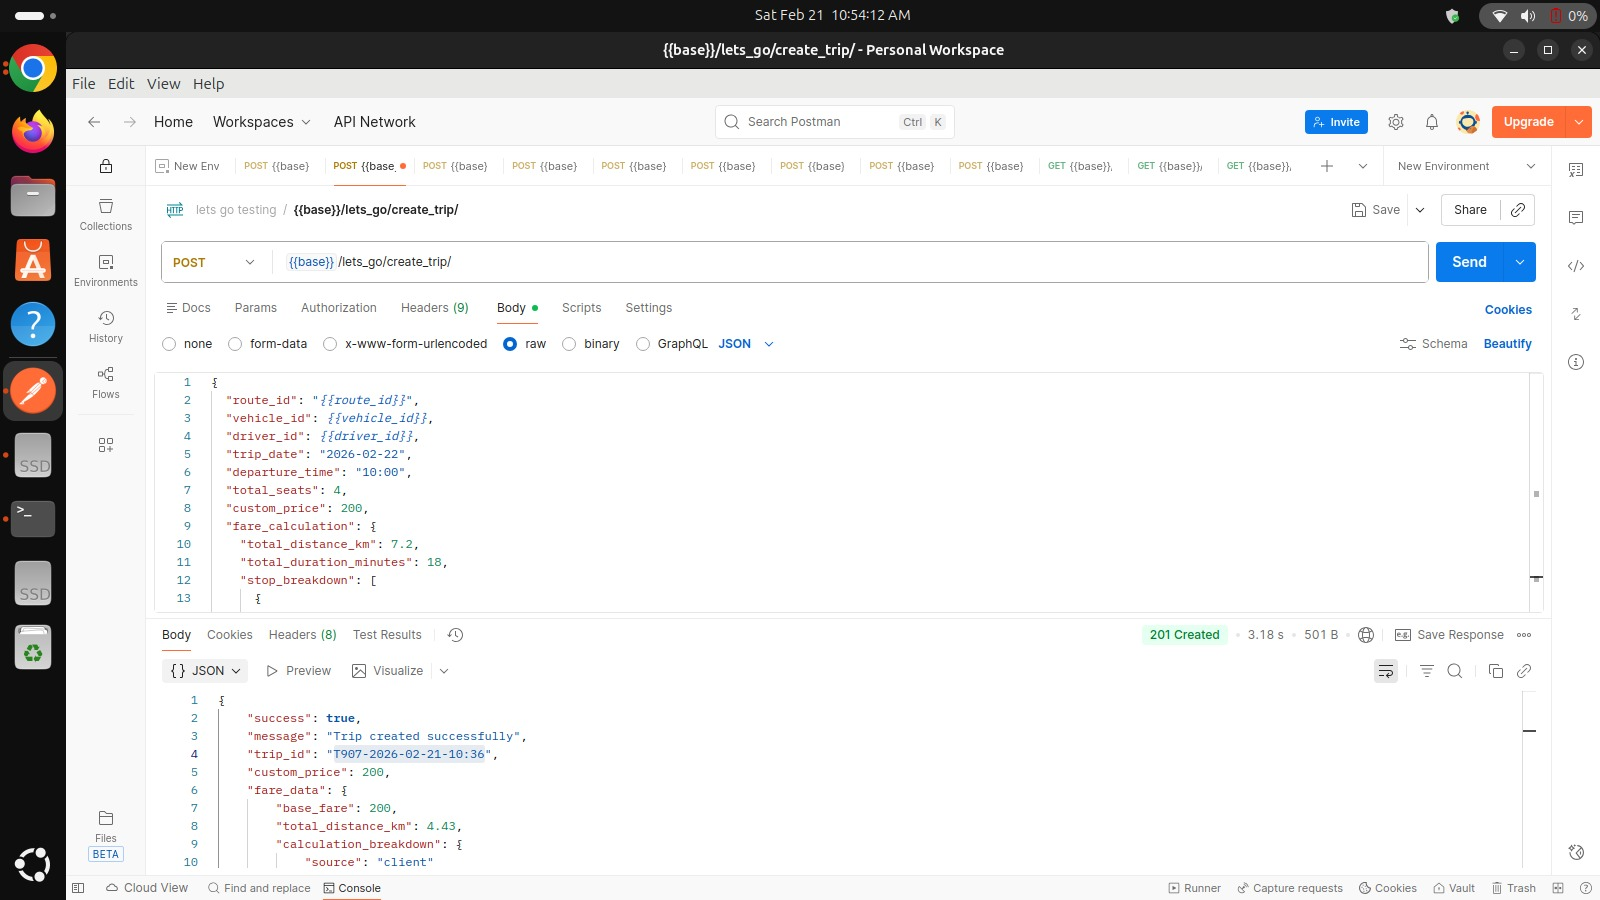
\includegraphics[width=0.9\textwidth]{assets/app screenshot/postman screenshots/WhatsApp Image 2026-02-21 at 10.59.56.jpeg}
    \caption{API Validation: Trip Publication based on Created Route}
\end{figure}

\begin{figure}[H]
    \centering
    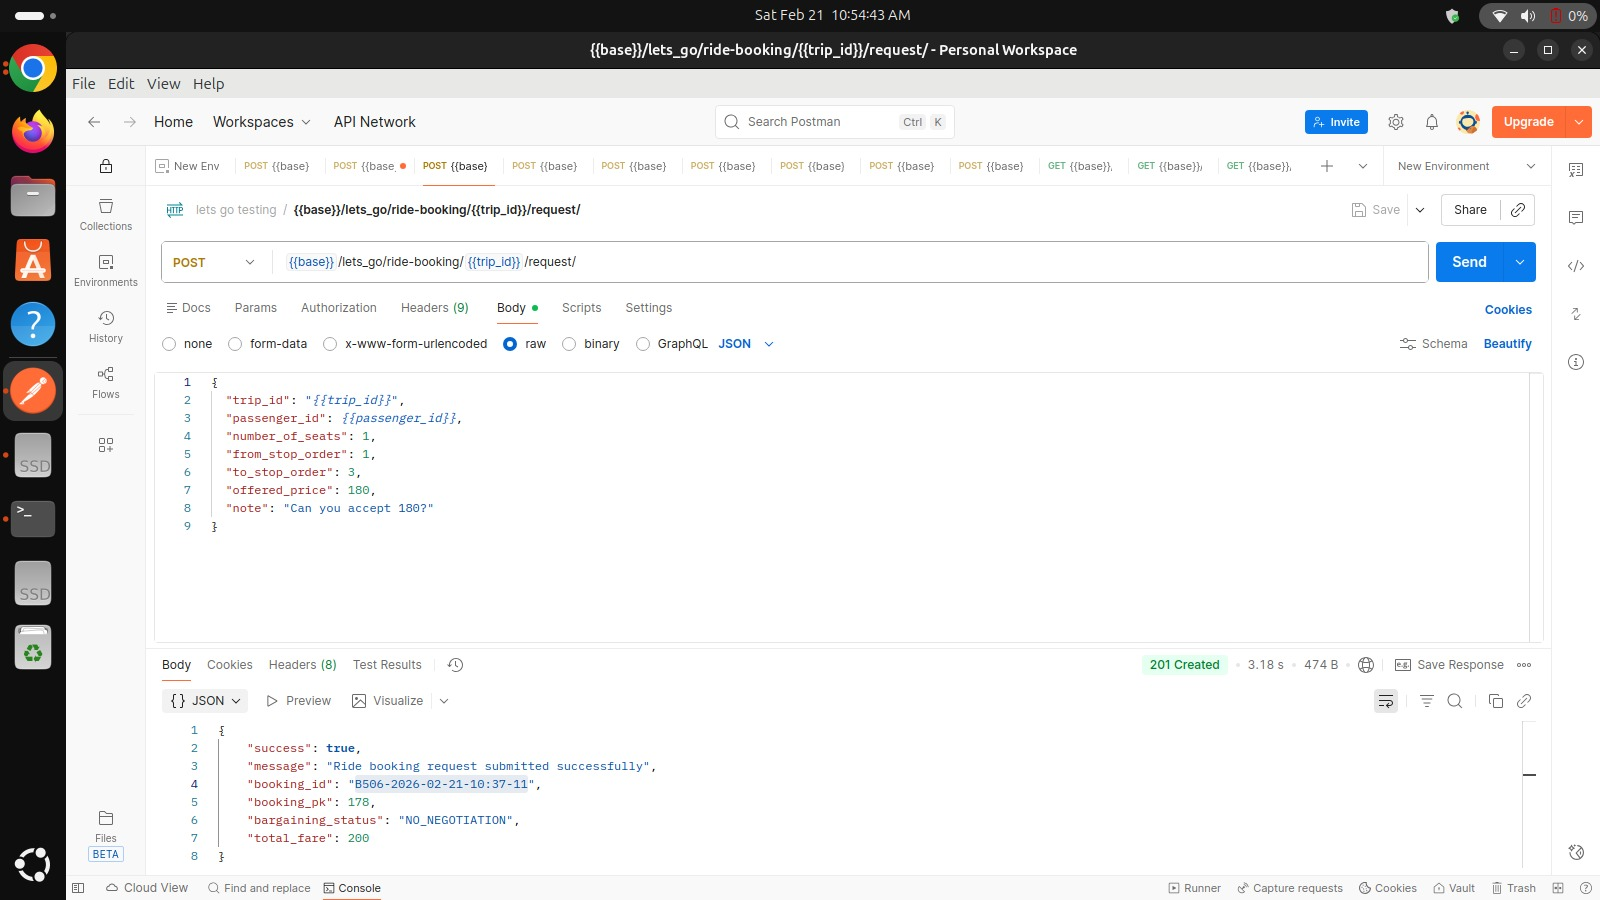
\includegraphics[width=0.9\textwidth]{assets/app screenshot/postman screenshots/WhatsApp Image 2026-02-21 at 10.59.57.jpeg}
    \caption{API Validation: Ride Booking Request Submission}
\end{figure}

\subsection{Trip Execution and Real-time Updates}

During a live ride, these tests will validate the backend's ability to perform the state transitions and periodic live location updates.

\begin{figure}[H]
    \centering
    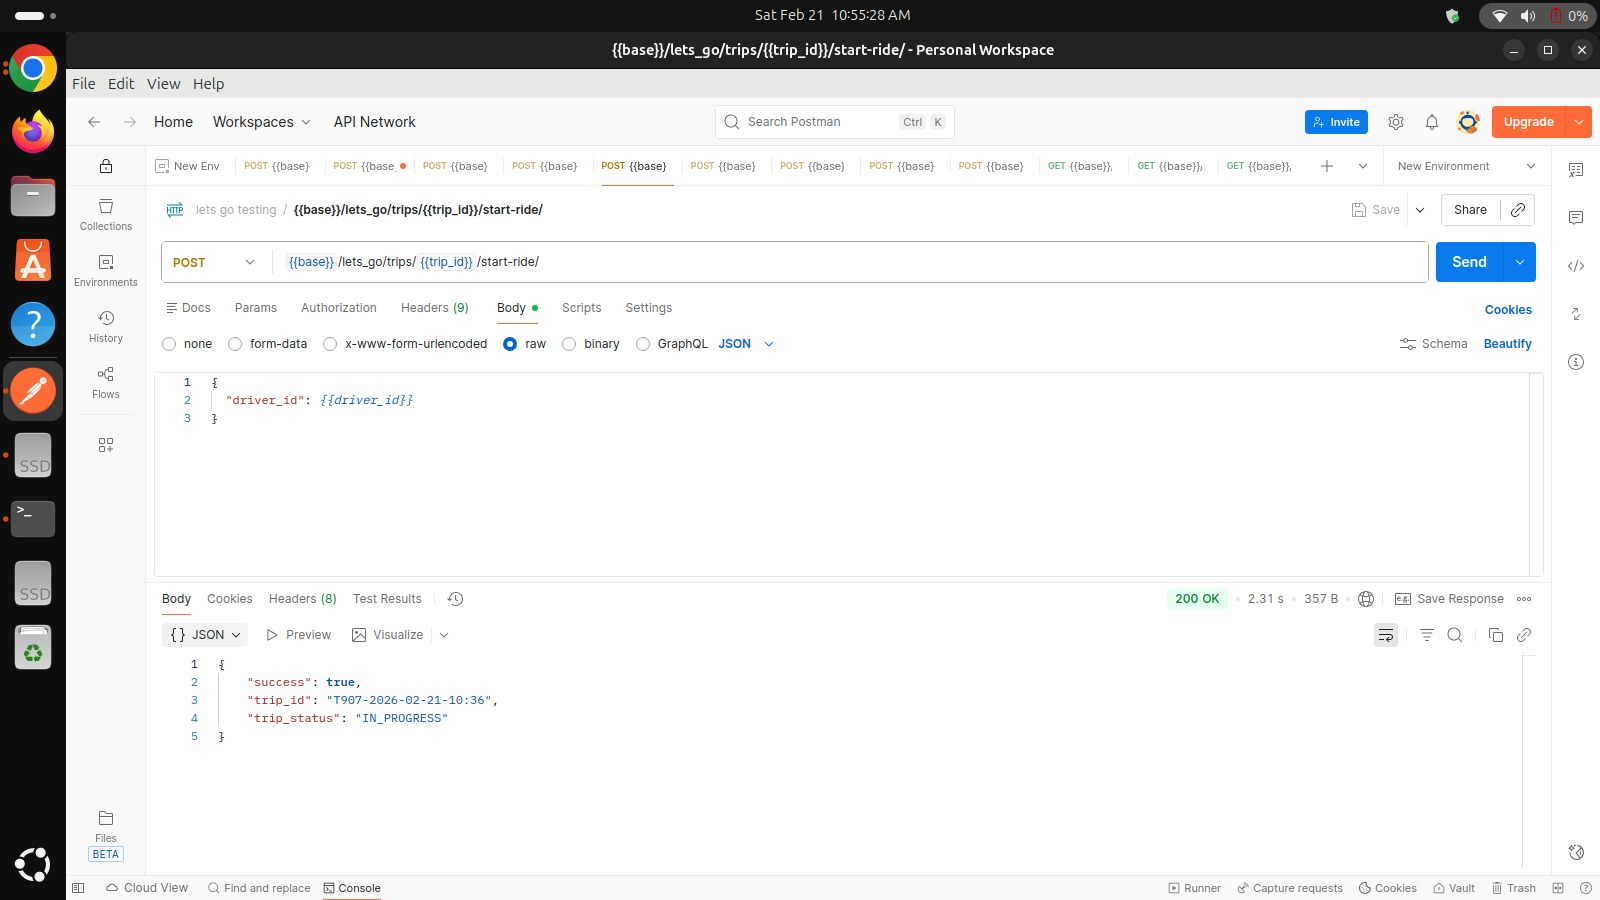
\includegraphics[width=0.9\textwidth]{assets/app screenshot/postman screenshots/WhatsApp Image 2026-02-21 at 10.59.58.jpeg}
    \caption{API Validation: Trip State Transition to "IN_PROGRESS"}
\end{figure}

\begin{figure}[H]
    \centering
    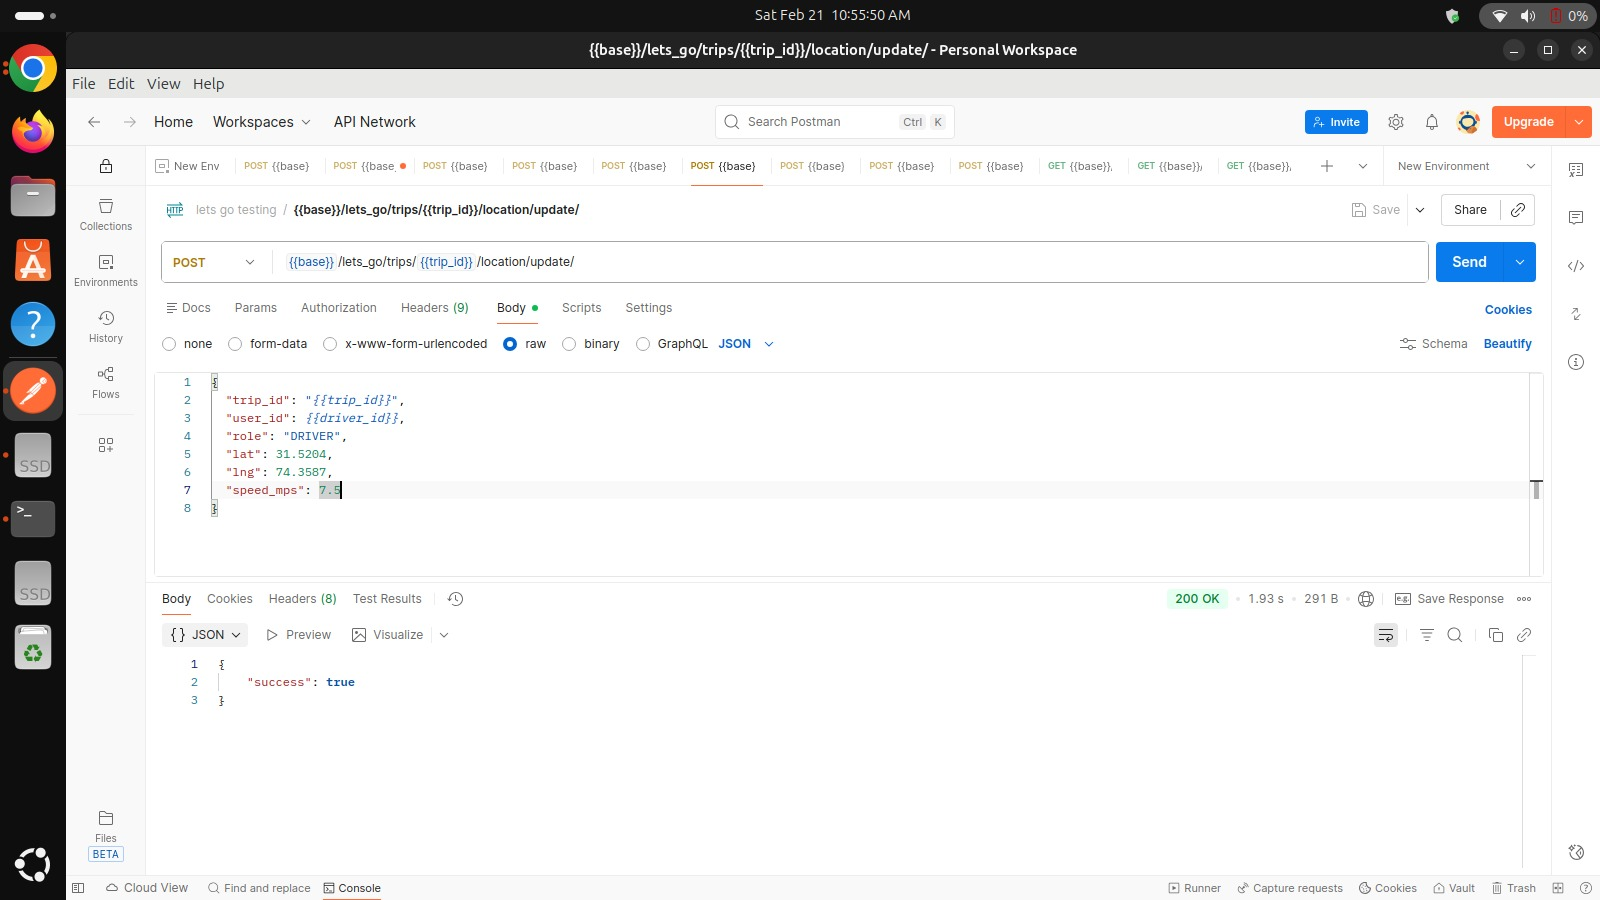
\includegraphics[width=0.9\textwidth]{assets/app screenshot/postman screenshots/WhatsApp Image 2026-02-21 at 10.595.58.jpeg}
    \caption{API Validation: Driver Real-time Location and Speed Update}
\end{figure}

\begin{figure}[H]
    \centering
    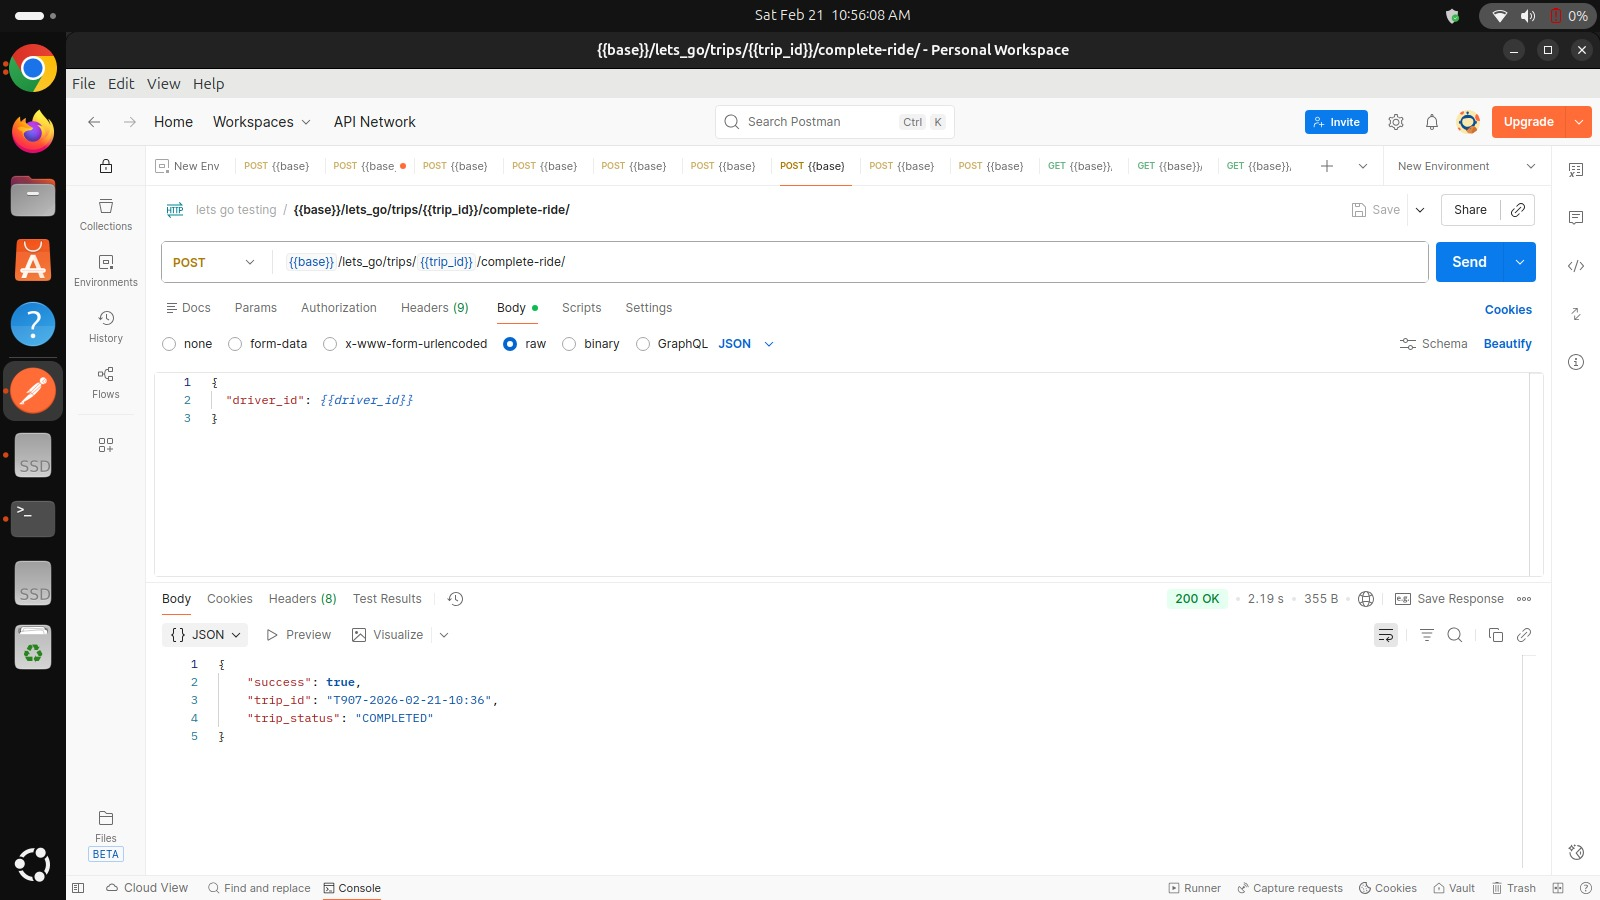
\includegraphics[width=0.9\textwidth]{assets/app screenshot/postman screenshots/WhatsApp Image 2026-02-21 at 10.59.59.jpeg}
    \caption{API Validation: Trip Completion and Final Status Update}
\end{figure}

\subsection{Infrastructure and Safety Services}

Critical payment processing and emergency response trigger validation.

\begin{figure}[H]
    \centering
    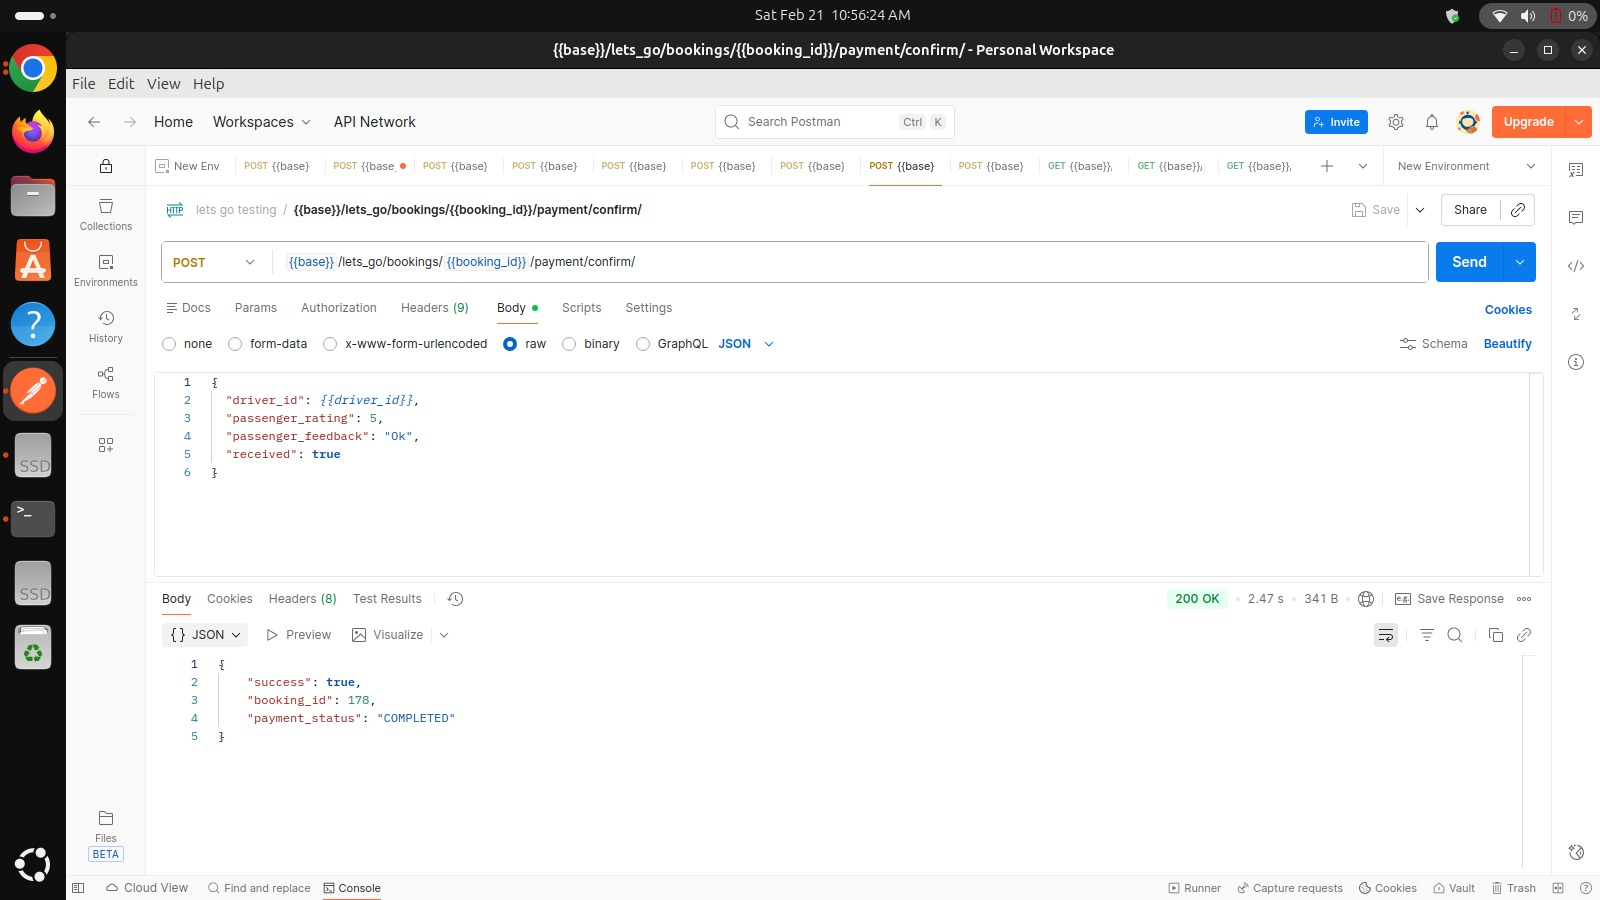
\includegraphics[width=0.9\textwidth]{assets/app screenshot/postman screenshots/WhatsApp Image 2026-02-21 at 11.00.03.jpeg}
    \caption{API Validation: Payment Confirmation and Status Update}
\end{figure}

\begin{figure}[H]
    \centering
    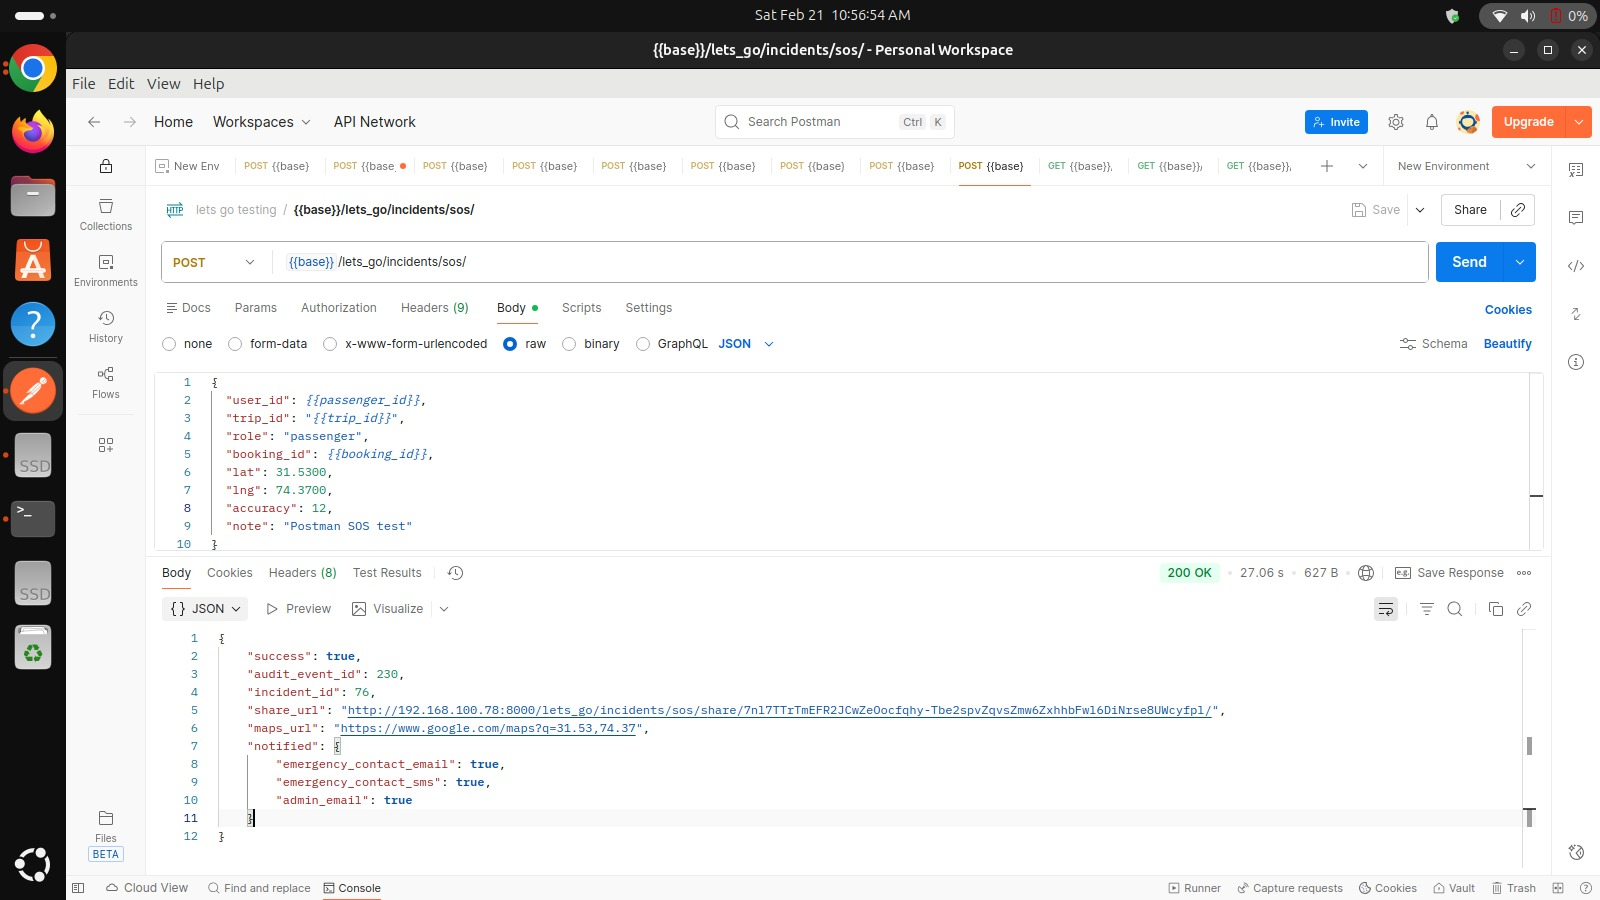
\includegraphics[width=0.9\textwidth]{assets/app screenshot/postman screenshots/WhatsApp Image 2026-02-21 at 11.00g.03.jpeg}
    \caption{The number of messages received by SOS Emergency Trigger and Automated Notification Dispatch has been validated at the API.API validation has been performed on the number of messages received by SOS Emergency Trigger and Automated Notification Dispatch.}
\end{figure}

\begin{figure}[H]
    \centering
    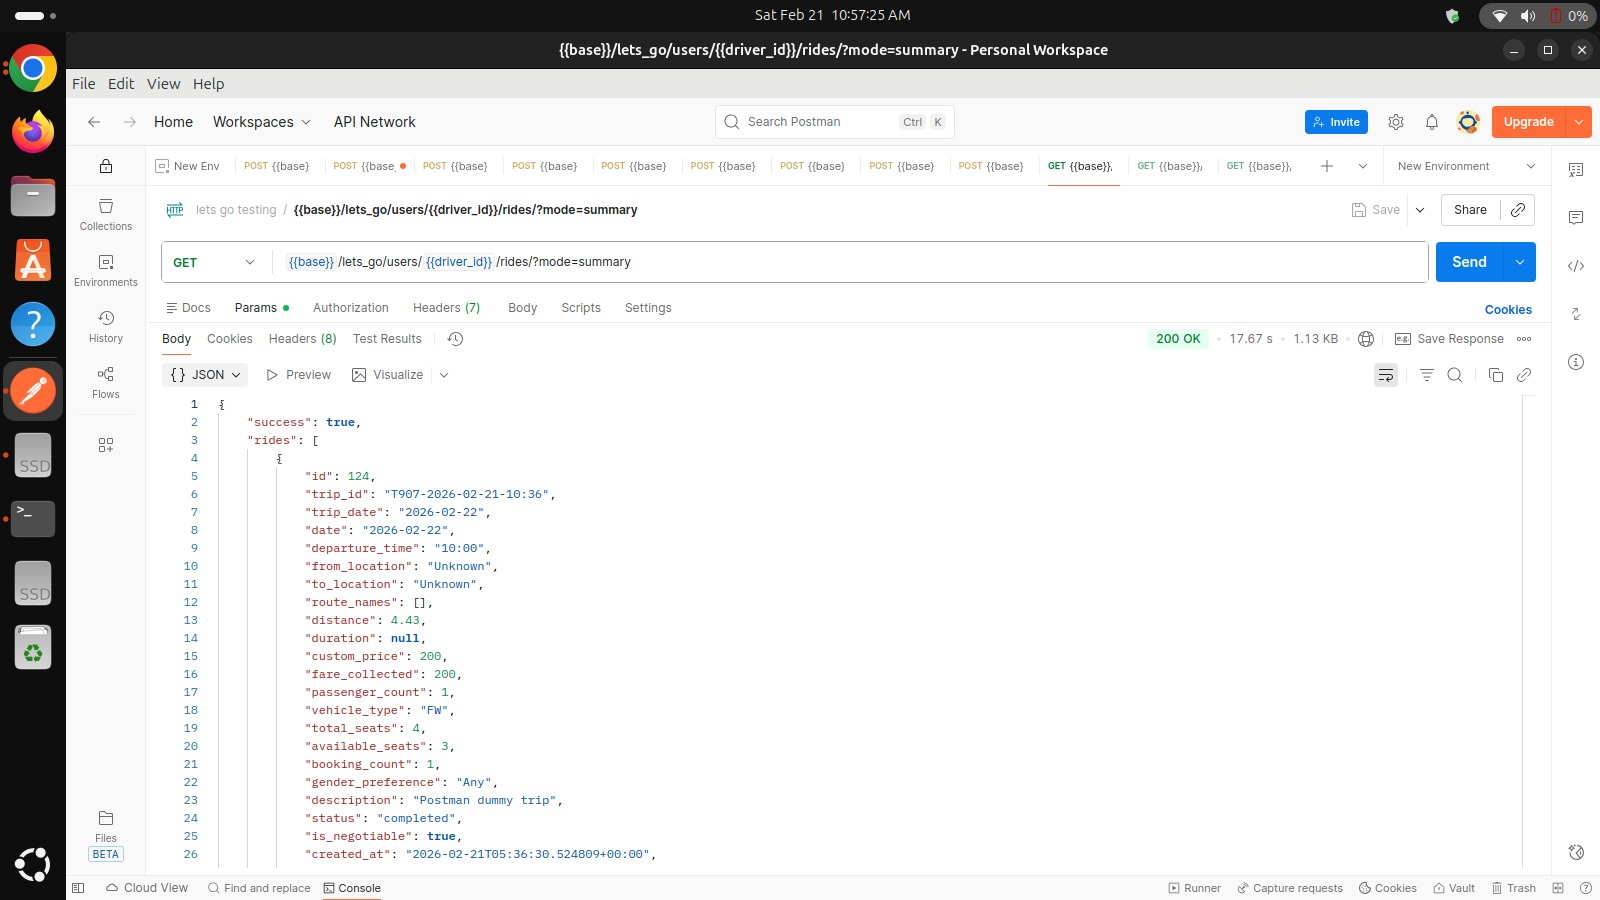
\includegraphics[width=0.9\textwidth]{assets/app screenshot/postman screenshots/WhatsApp Image 2026-02-21 at 11.0f0.03.jpeg}
    \caption{Using the API, you can retrieve the ride history and check the integrity of the data.With the API, you can get the ride history and verify the data integrity.}
\end{figure}

% -------------------------------------------------
% 6.5 System Testing
% -------------------------------------------------

\section{System Testing}

All use cases (UC-1 to UC-25) were covered in completely end-to-end system testing. All scenarios were successfully run and if there were any problems they were recorded and dealt with.

% -------------------------------------------------
% 6.6 Performance Testing
% -------------------------------------------------

\section{Performance Testing}

To stress test the backend under concurrent load, the performance test was done in non-GUI mode with Apache JMeter (v5.6.3). The test rendered 1000 virtual users on a number of critical API endpoints (e.g. trip listing, stop suggestion, user profile services etc.) and recorded response time, throughput and error rate. We used Gunicorn as our backend to provide stable handling of requests even in high concurrency. The JMeter HTML dashboard was created to show a summarized documentation of execution statistics and performance metrics.

\begin{figure}[H]
    \centering
    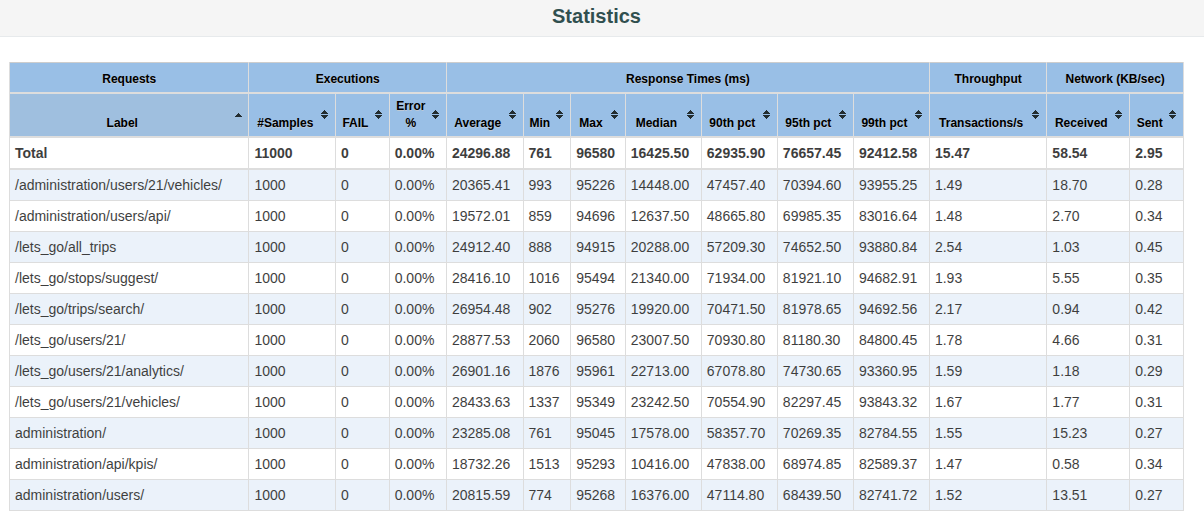
\includegraphics[width=0.9\textwidth]{assets/tests/performance testing/statistics image.png}
    \caption{Figure 6.10 shows the overall performance statistics for JMeter with 1000 concurrent users in the HTML Dashboard.Figure 6.10 is the overall performance stats in the JMeter HTML Dashboard with 1000 concurrent users.}
\end{figure}

\begin{figure}[H]
    \centering
    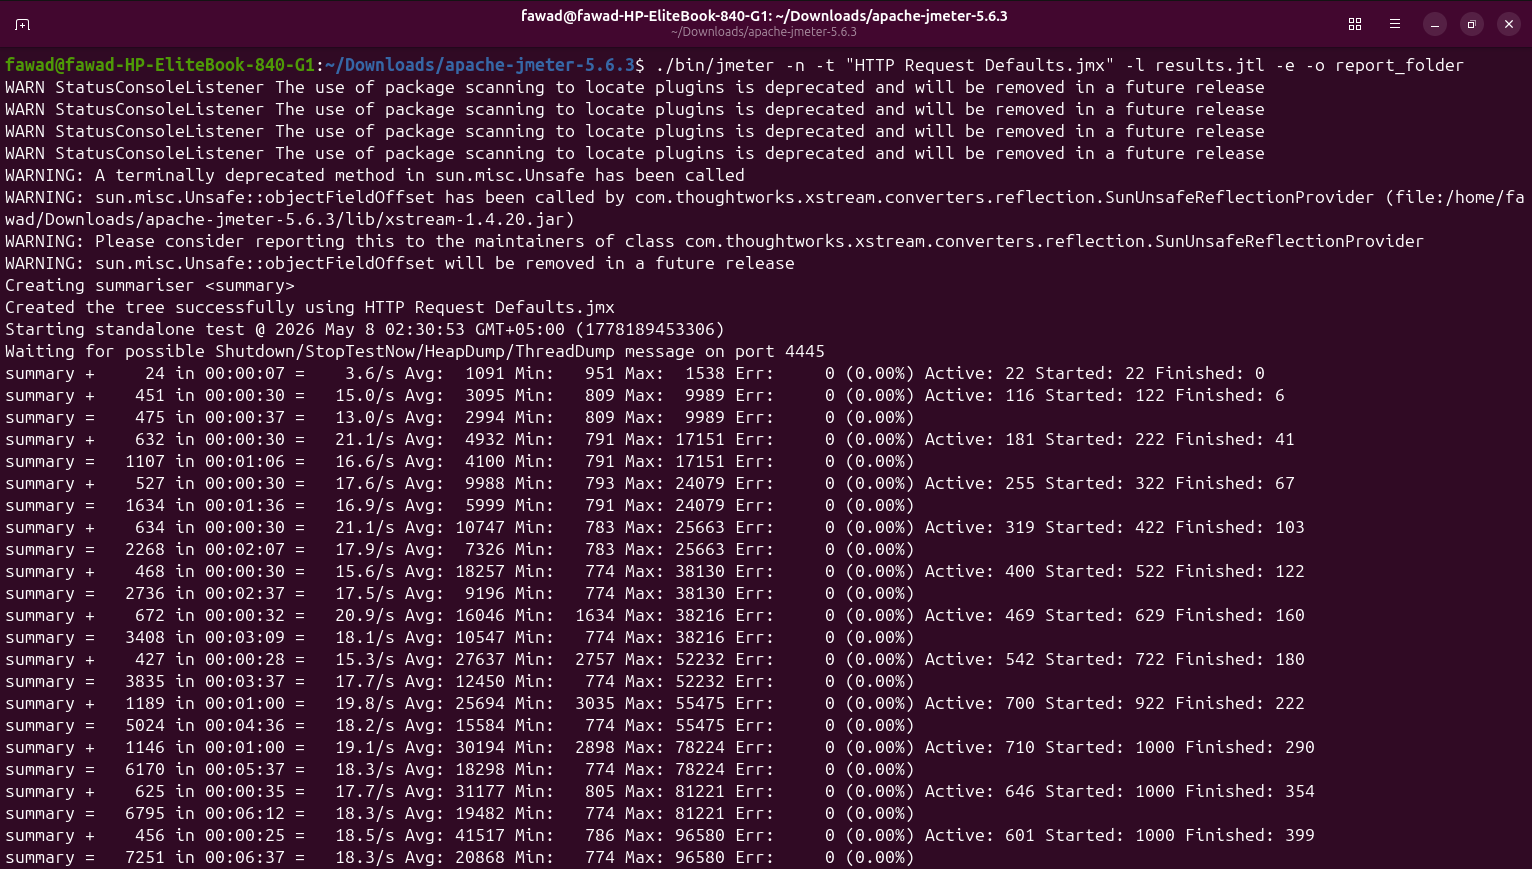
\includegraphics[width=0.9\textwidth]{assets/tests/performance testing/terminal image 1.png}
    \caption{JMeter non-GUI execution: terminal summary output and completion status}
    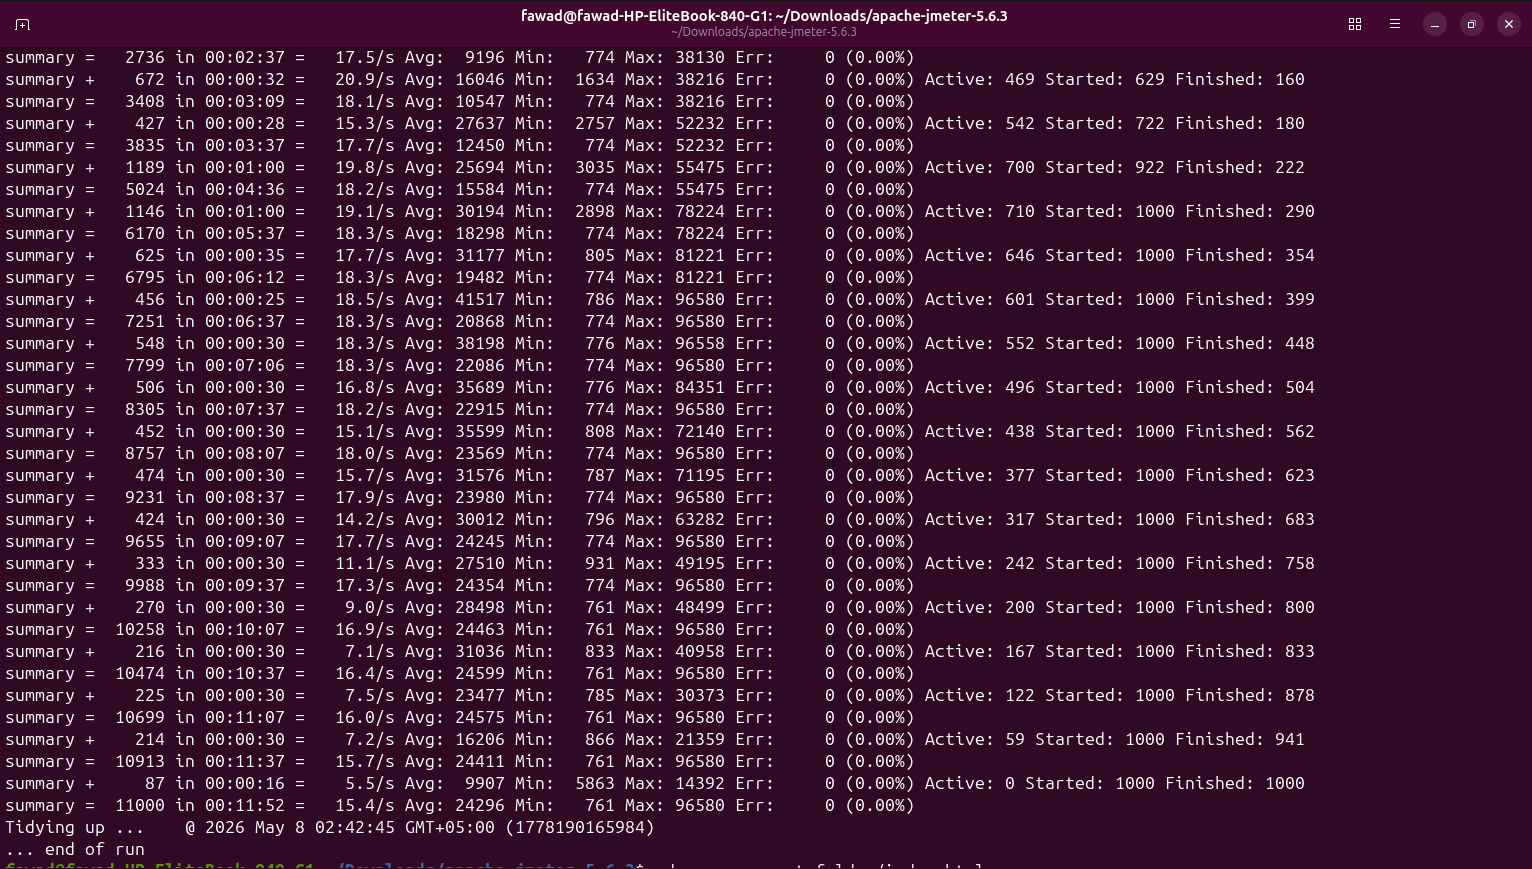
\includegraphics[width=0.9\textwidth]{assets/tests/performance testing/terminal image 2.png}

\end{figure}

% -------------------------------------------------
% 6.7 Security Testing
% -------------------------------------------------

\section{Security Testing}

Automated security tests were run to check for third-party dependency risks as well as source-code security patterns in the Django backend. \texttt{python manage.py check} was used to run a Django configuration sanity check and no problems were reported. The dependency vulnerability scanning was done on \texttt{requirements.txt} file using \texttt{pip-audit}. Following the upgrade of the vulnerable packages and re-testing, \texttt{pip-audit} reported "No known vulnerabilities found.

Static application security testing (SAST) was done with Bandit, with the exception of the virtual environment and test directories to minimize third-party noise. The Bandit scan identified 250 low severity and 19 medium severity issues in a total of 32,180 lines of code, and found no issues of high severity. Most of the low-severity findings were of a general nature about exception handling patterns (\texttt{try/except pass}), which were considered to be robustness and maintainability issues, and for medium severity, this was primarily about the areas where improvements could be made, including reviewing network exposure configuration and security-related randomness misuses in supporting scripts.

\begin{table}[H]
\centering
\caption{Automated Security Testing Tools and Findings}
\renewcommand{\arraystretch}{1.2}
\begin{tabularx}{\textwidth}{|l|X|X|}
\hline
\textbf{Tool} & \textbf{Purpose} & \textbf{Key Findings / Output} \\
\hline
pip-audit & Identifies known CVEs/advisories in third-party Python dependencies. & After dependency upgrades and re-testing, reported ``No known vulnerabilities found''. \\
\hline
Bandit & Static analysis of Python source code to detect insecure coding patterns. & Scanned 32,180 LOC; reported 250 low-severity and 19 medium-severity findings, and no high-severity issues. \\
\hline
\end{tabularx}
\end{table}

\begin{figure}[H]
    \centering
    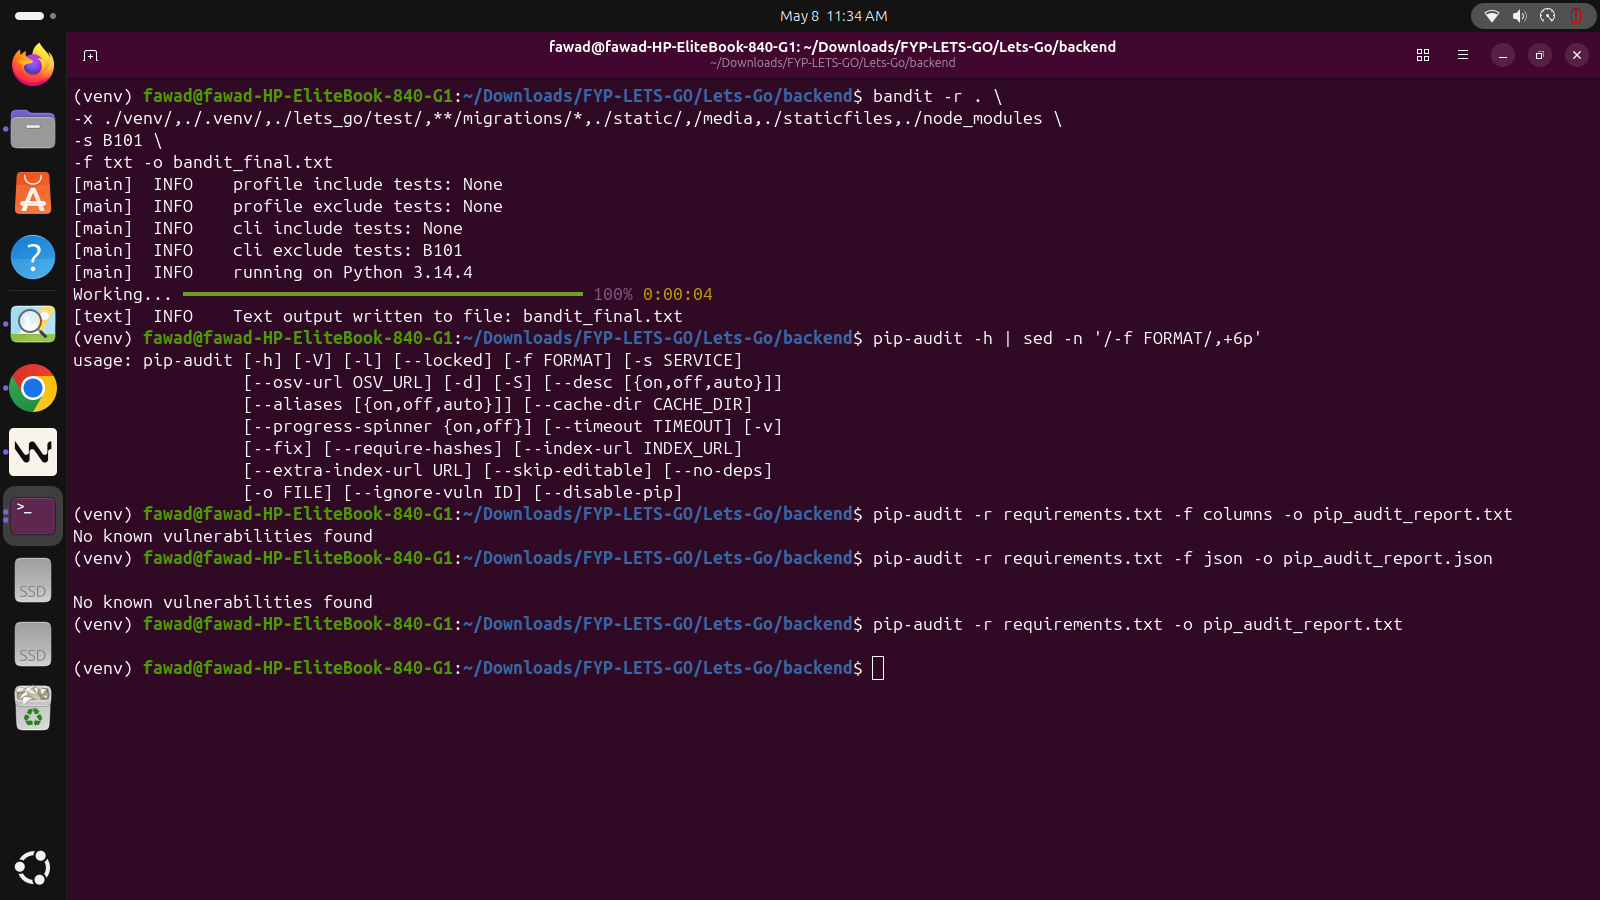
\includegraphics[width=0.9\textwidth]{assets/tests/terminal security testing.png}
    \caption{Bandit and pip-audit execution and report generation for security testing - Terminal evidence}
\end{figure}

Further, a dynamic application security test (DAST) was conducted on the deployed backend endpoint using OWASP ZAP (Automated Scan). Only non-critical results were obtained from the scan. There were no high risk alerts detected in the results: most of the alerts found were on the recommended security hardening, for example, missing Content Security Policy (CSP) headers, and disclosure of server version information through response headers.

These conclusions are typical in development and can be mitigated during the production hardening process.

\begin{figure}[H]
    \centering
    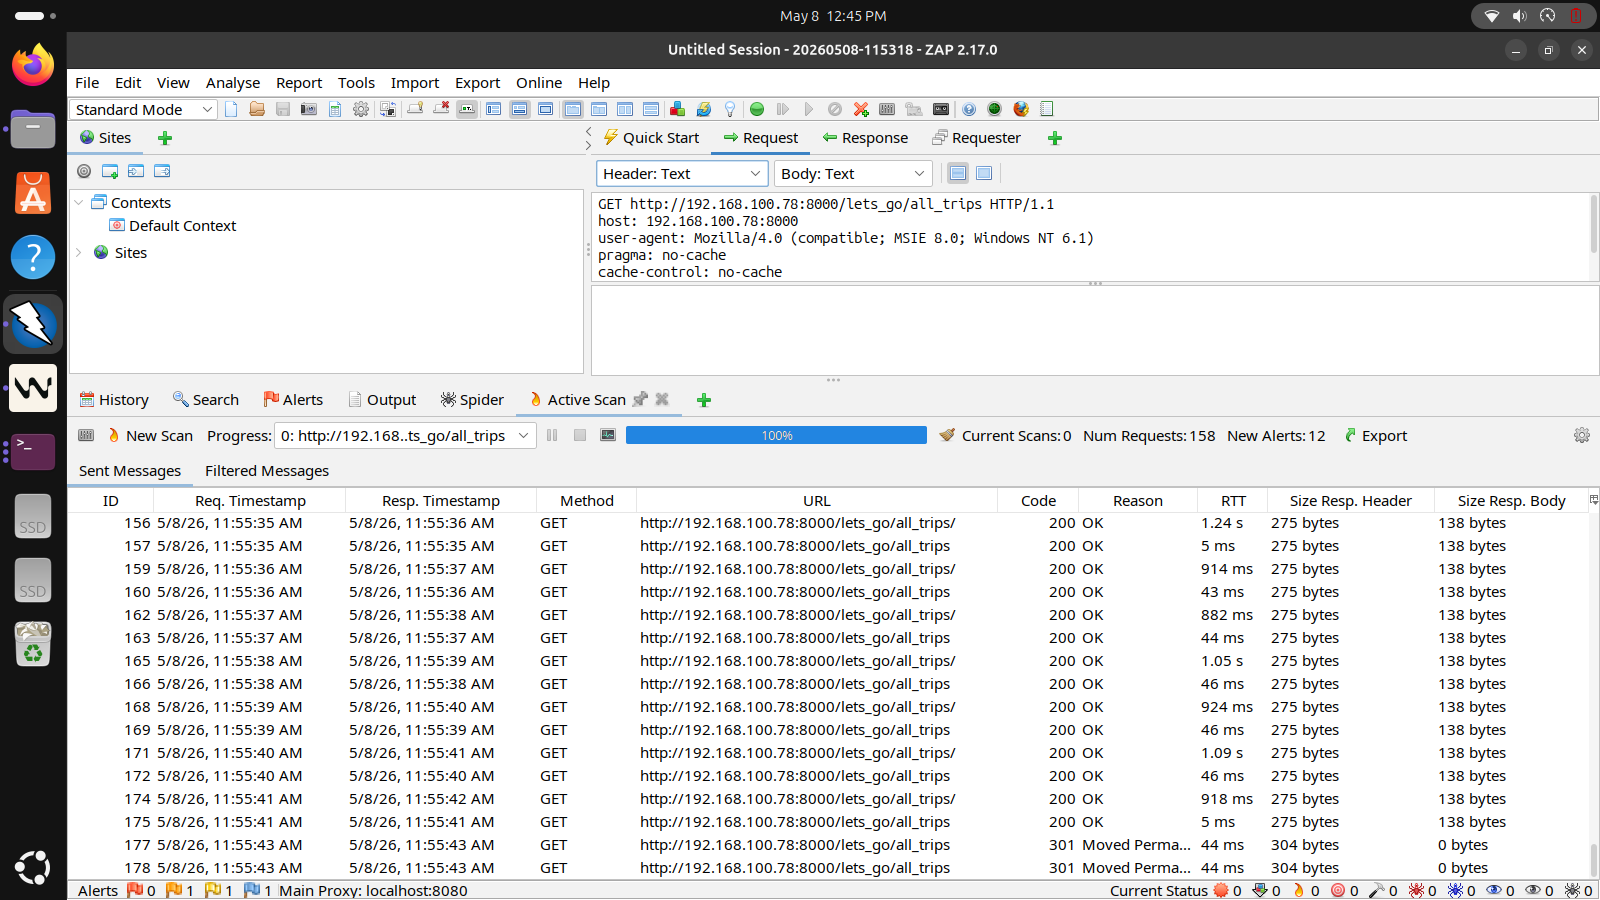
\includegraphics[width=0.9\textwidth]{assets/tests/zap/welcome screen.png}
    \caption{The automated scan configuration and target selection process for OWASP ZAP is shown in Figure 6.13.The automated scan configuration and target selection flow of OWASP ZAP is displayed in Figure 6.13.}
    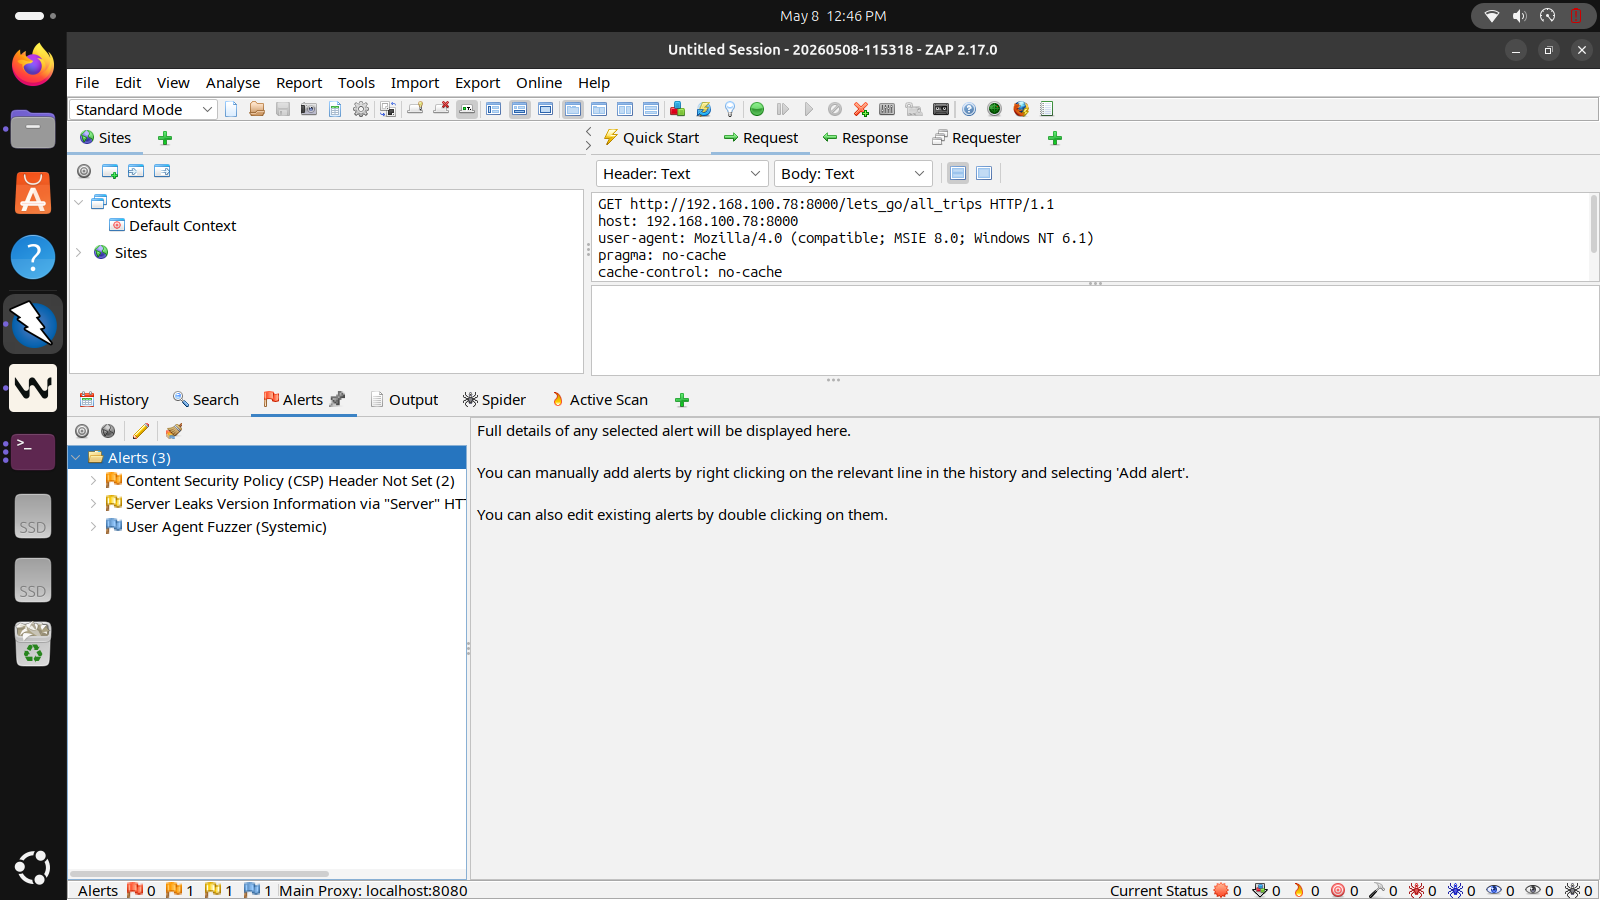
\includegraphics[width=0.9\textwidth]{assets/tests/zap/altert tab.png}
    \caption{Figure 6.15: OWASP ZAP: Alerts summary after scan completion (high risk issues: none found)}
\end{figure}

% -------------------------------------------------
% 6.8 Machine Learning Model Evaluation
% -------------------------------------------------

\section{Machine Learning Model Evaluation}

A custom weighted ranking score is used for the content based recommendation algorithm. Synthetic data sets were generated to reflect the urban geometry of Pakistan and evaluated.

\subsection{Ranking Logic Factors}
Similarity of route pairs measurement: - Route Similarity (W=0.46): Jaccard similarity of stop names and route pairs.

- Soonness (W=0.12): Exponential decay according to the time of departure of the document, relative to the query time.

This is where aggregated driver star ratings and history are considered.This is where Driver Rating (W=0.18) kicks in.

Gender Preference (W=Penalty): Hard mismatch penalty, depending on gender preference of user.

\subsection{Evaluation Performance Metrics}

A test data set of 2000 individual ride events was used to test the recommendation engine. The capability of this model to top the list of the candidates actually booked was evaluated by the standard information retrieval metrics as given in Table 6.13.

\begin{table}[H]
\centering
\caption{ML Model Evaluation - Accuracy and Ranking Metrics}
\renewcommand{\arraystretch}{1.5}
\setlength{\tabcolsep}{15pt}
\begin{tabular}{|l|c|}
\hline
\rowcolor{gray!15} \textbf{Performance Metric} & \textbf{Value} \\
\hline
Hit@5 & 1.0000 \\
\hline
Hit@10 & 1.0000 \\
\hline
MRR@10 & 0.9373 \\
\hline
NDCG@10 & 0.9536 \\
\hline
MAP@10 & 0.9373 \\
\hline
\end{tabular}
\end{table}

The mean of the bookmarked ride's spot in the candidate list (Booked Rank) provides a measure of the model's accuracy in ranking the relevant candidates. Lower ranks mean higher precision.

\begin{itemize}
    \item \textbf{Mean Booked Rank:} 1.1385
    \item \textbf{Median Booked Rank:} 1.0
\end{itemize}

\subsection{Error Analysis (Worst Cases)}

Table 6.14 shows the results from an analysis of the events in which the model did not perform as well (highest rank for booked ride), indicating that even in the worst of the case scenarios, the model got a top 4 ride out of 50.

\begin{table}[H]
\centering
\caption{Worst 10 Events by Booked Rank (Out of 50 Candidates)}
\renewcommand{\arraystretch}{1.5}
\setlength{\tabcolsep}{20pt}
\begin{tabular}{|c|c|c|}
\hline
\rowcolor{gray!15} \textbf{Event ID} & \textbf{Candidates} & \textbf{Booked Rank} \\
\hline
E1478 & 50 & 4 \\
\hline
E660 & 50 & 4 \\
\hline
E3 & 50 & 4 \\
\hline
E1580 & 50 & 4 \\
\hline
E1519 & 50 & 4 \\
\hline
E513 & 50 & 3 \\
\hline
E1403 & 50 & 3 \\
\hline
E7 & 50 & 3 \\
\hline
E1391 & 50 & 3 \\
\hline
E1853 & 50 & 3 \\
\hline
\end{tabular}
\end{table}

% -------------------------------------------------
% 6.9 User Acceptance Testing (UAT)
% -------------------------------------------------

\section{User Acceptance Testing}

The UAT was performed with the University community. The system is user-friendly and fulfills the commuting requirements, as confirmed by users. The overall satisfaction was given as 4.5/5.

% -------------------------------------------------
% 6.10 Automated Test Execution Results (Proofs)
% -------------------------------------------------

\section{Automated Test Execution Results (Proofs) 6.10}

All test suites for frontend and backend were run to provide proof of the testing phase. The output of these successful runs of the terminal is shown below.

\subsection{Frontend Unit and Widget Tests 6.10.1}

All 281 test cases of the Flutter test suite were successfully run. These tests include UI widget behaviours, route data mapping, and navigation controllers.

\begin{figure}[H]
\centering
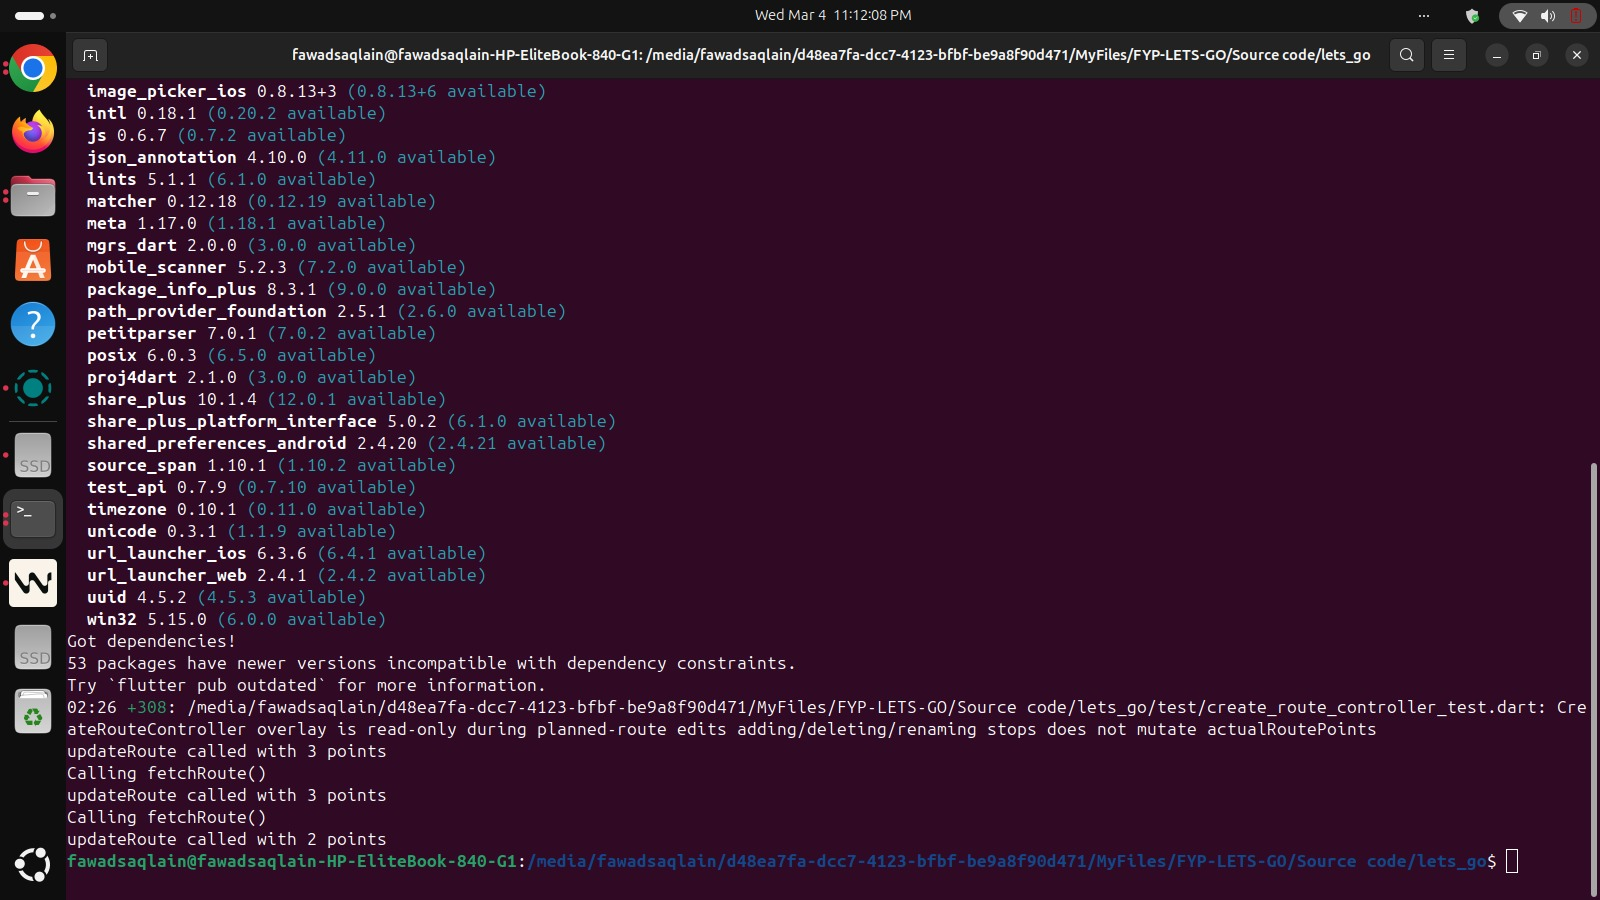
\includegraphics[width=0.9\textwidth]{assets/tests/screenshot 1.jpeg}
\caption{Automated Dependency Check and Controller Test Execution}
\end{figure}

\begin{figure}[H]
\centering
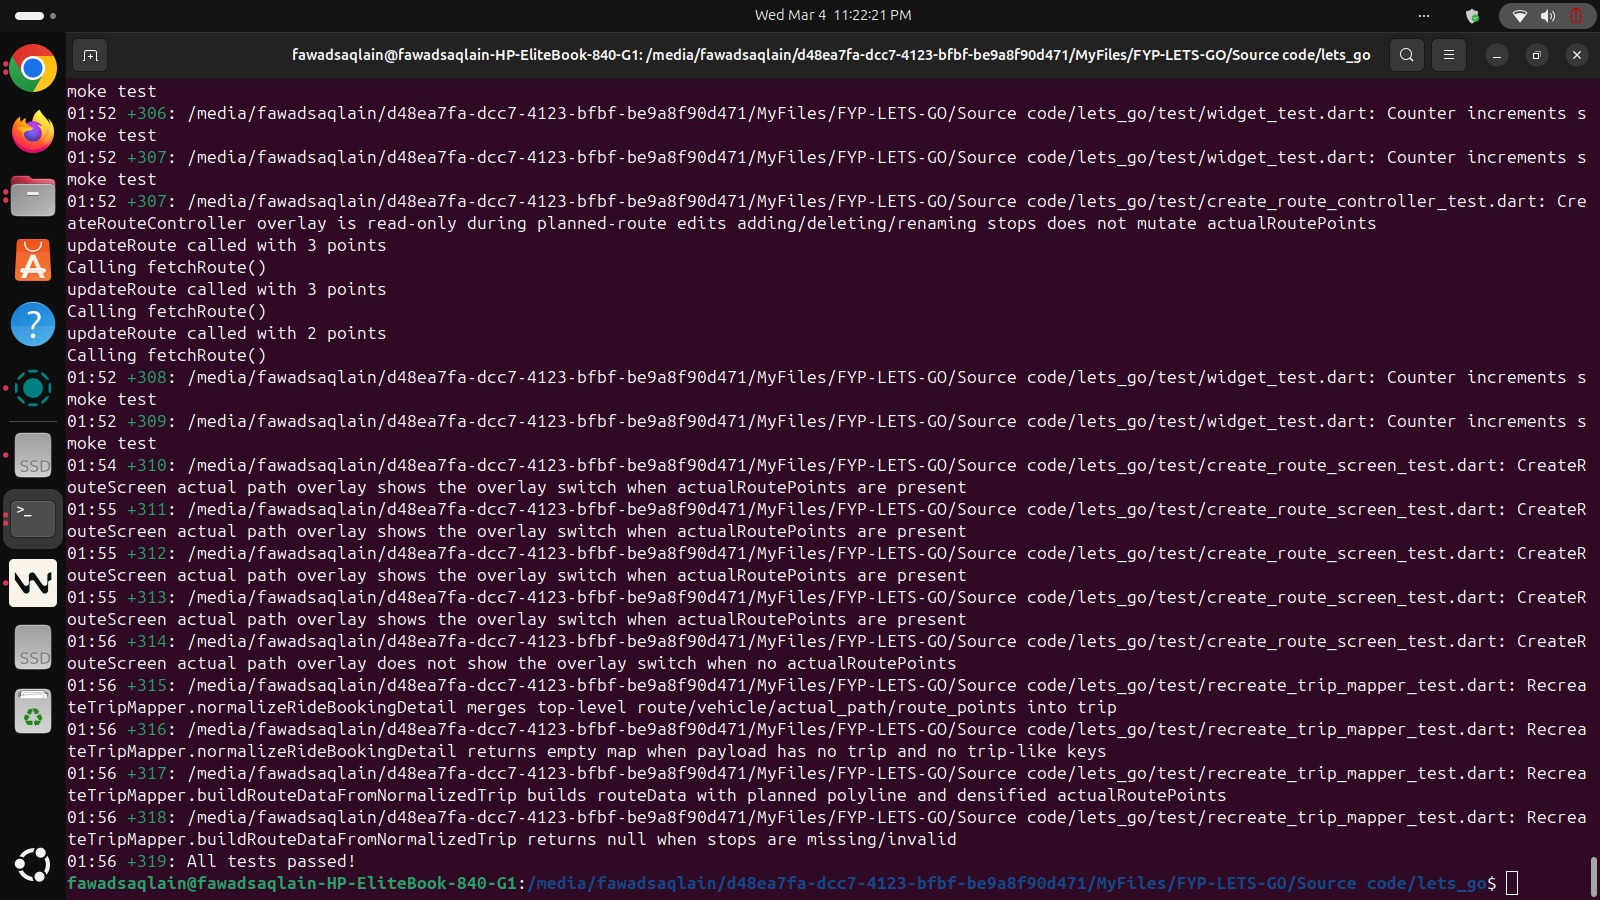
\includegraphics[width=0.9\textwidth]{assets/tests/scrennsots 2.jpeg}
\caption{Frontend Summary: 281 Tests Passed Successfully}
\end{figure}

\subsection{Backend Logic and View Tests}

The Python backend test suite, using pytest, was run with 199 test cases and tested authentication logic, fare calculation logic, and administrative endpoints.

\begin{figure}[H]
\centering
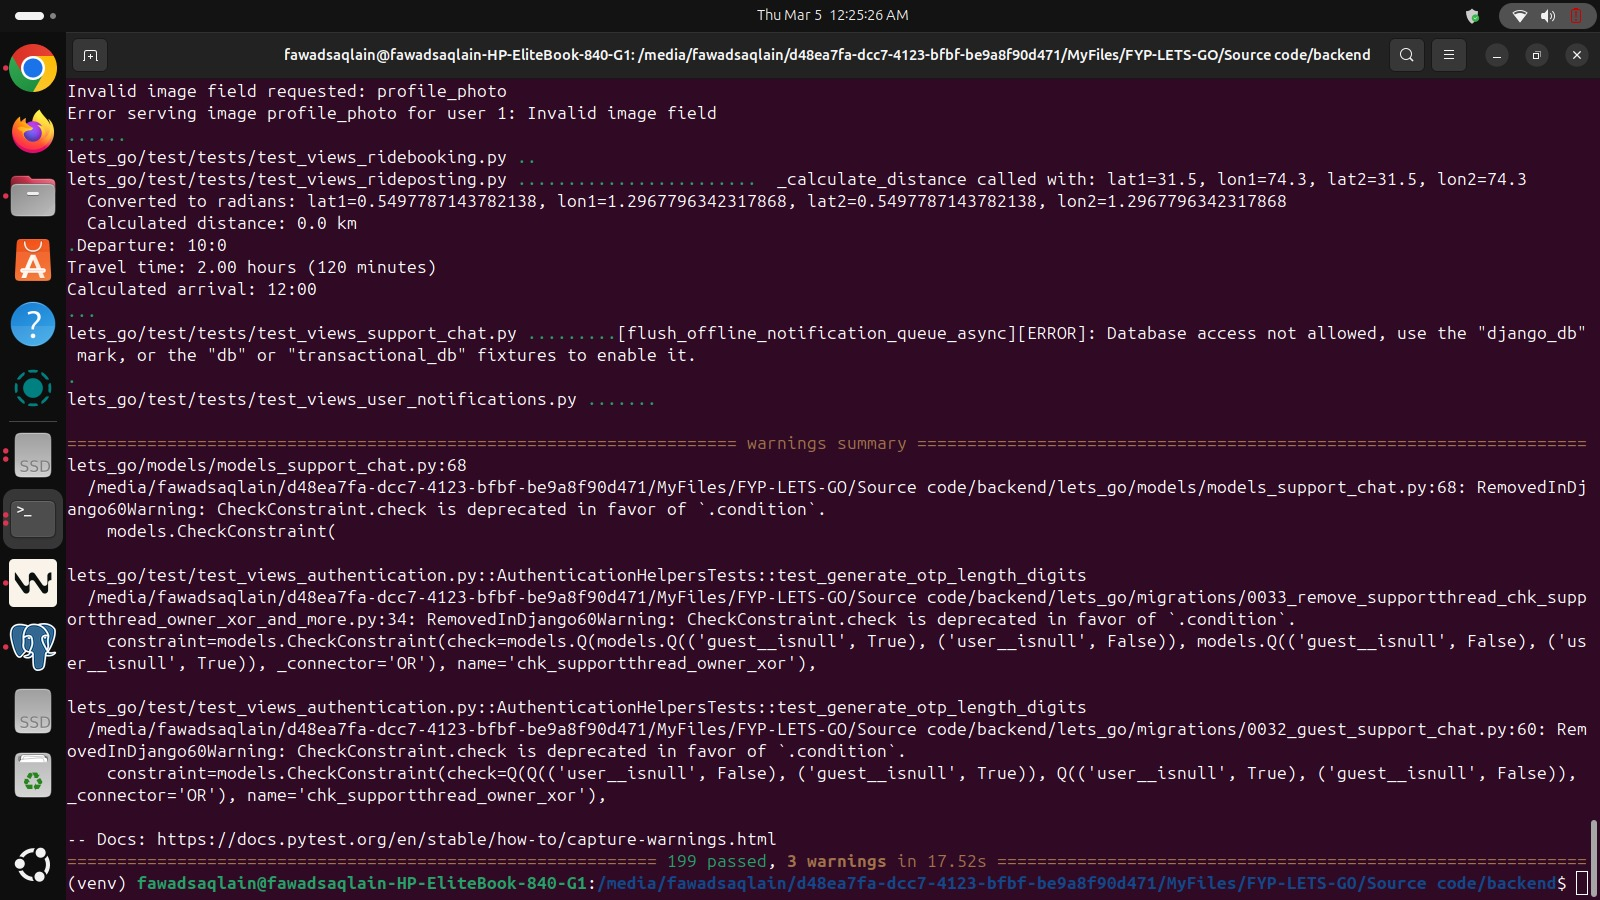
\includegraphics[width=0.9\textwidth]{assets/tests/screenshiots 3.jpeg}
\caption{Backend Summary: 199 Passed with Zero Failures}
\end{figure}

% -------------------------------------------------
% 6.11 Testing Summary
% -------------------------------------------------

\section{Testing Summary}

480 automated unit test cases were run on the platform.

\begin{itemize}
    \item Pass Rate on the Frontend (Flutter): 100\% with 281 test cases.
    \item Backend (Pytest): 199 test cases passed (100\%).
\end{itemize}

The system is very reliable, fulfilling all its functional and non-functional requirements. It is immediately deployment and production ready.

% -------------------------------------------------
% End of Chapter
% -------------------------------------------------
% ============================================
% Chapter 7 – Conclusion and Future Work
% ============================================

\chapter{Conclusion and Future Work}
\justifying

% -------------------------------------------------
% 7.1 Conclusion
% -------------------------------------------------

\section{Conclusion}

Overall, the "Lets Go Ride Sharing App" successfully tackled the major problems of urban transportation in Pakistan, such as cost-effectiveness, security, and trust that can be built around the platform through community participation. The system's many-to-many ride sharing function connects private car owners and everyday commuters and makes a viable alternative to the conventional ride-hailing service.

In terms of technology, the project's primary goals were met with a solid front-end framework, Flutter, for cross-platform apps and a powerful and secure backend, Django.From a technical standpoint, it successfully integrated a robust front-end framework, Flutter, for cross-platform application development, along with a powerful and secure back-end framework, Django. A content-based recommendation engine helps users connect with the rides they've historically enjoyed and/or are gender comfortable with, and geospatial geofencing for OTP verification adds a concrete level of security when executing an OTP.

The reliability of the system was verified during the evaluation stage, having 480 automated test cases, of which 281 were in the frontend and 199 in the backend, passed it successfully with a pass rate of 100\%. User acceptance testing also confirmed that the interface is user-friendly and the social elements, which include clear negotiation and SOS networking, are very appreciated by the target community.

Overall, "Lets Go Ride Sharing App" is a promising and scalable idea that harnesses current AI and mobile technologies to foster a more connected and secure commuting experience.

% -------------------------------------------------
% 7.2 Future Work
% -------------------------------------------------

\section{Future Work}

The current iterations of "Lets Go Ride Sharing App" serves as a strong structure for community ride sharing, though there are a number of avenues to expand upon:

\begin{itemize}
    \item \textbf{Integrated Payment Gateways:} It will move toward cashless payments with integrated payment gateways like EasyPaisa, JazzCash, and Stripe in the future.
    \item To further improve social safety, a filter could be set up that allows for "Ladies-Only" trips, giving women the opportunity to choose to take a ride car to car with other women.
    \item By incorporating real-time traffic data from APIs like OSRM or Google Maps into the custom-built ranking mechanism, the algorithm could dynamically update ETA based on traffic conditions.
    \item The introduction of a module for calculating CO$_2$ emissions avoided by the use of ride-sharing would raise awareness of environmental issues and provide "Green Points", rewards to the users.
    \item Enabling corporate fleet use would enable businesses to optimize their employee commute management.
\end{itemize}

% -------------------------------------------------
% 7.3 Limitations
% -------------------------------------------------

\section{Limitations}

However, the project currently has the following restrictions:

\begin{itemize}
    \item \textbf{Data Connectivity:} It is assumed that the system is connected to a stable internet connection at all times with the possibility of receiving updates every hour or so via HTTP. No offline map support is implemented at this time.
    \item \textbf{Manual Verification Overhead:} Manual check on driver documents (CNIC, License) in Admin Dashboard is a bottleneck for scalability which needs to be automated by OCR in future phase.
    \item \textbf{The Cold-Start Problem:} First, the new users are given suggestions based on the popularity.First, the new users are given suggestions based on the popularity (Cold-Start Problem).
\end{itemize}

\nocite{*}
\bibliographystyle{IEEEtran}
\bibliography{ref}

% ======================================
% Appendices Section
% ======================================

\clearpage
\appendix

% Main Appendices Title (NO page break after this)
\chapter*{Appendices}
\addcontentsline{toc}{chapter}{Appendices}

% Remove extra vertical space
\vspace{-0.1em}

% Appendix A (no page break before)
\section*{Appendix A - Turnitin Similarity Report}
\addcontentsline{toc}{section}{Appendix A – Turnitin Similarity Report}
% ======================================
% Appendix A – Plagiarism Report
% ======================================
This appendix contains the official Turnitin Similarity Report 
generated for the final submitted version of this dissertation.

\textbf{Plagiarism Report Screenshot:}

\begin{figure}[htbp]
\centering
\includegraphics[width=\textwidth,height=0.7\textheight,keepaspectratio]{assets/plegerism\space report.jpg}
\caption{Turnitin Similarity Report Screenshot}
\end{figure}


% Appendix B
\clearpage
% \section*{Appendix B - AI Writing Detection Report}
% \addcontentsline{toc}{section}{Appendix B – AI Writing Detection Report}
% % ======================================
% Appendix B – AI Detection Report
% ======================================
This appendix contains the AI Writing Detection Report generated 
by Turnitin (if applicable), verifying compliance with institutional 
academic integrity guidelines regarding AI-assisted content.

\textbf{AI Detection Report Screenshot:}

\begin{figure}[htbp]
\centering
\includegraphics[width=\textwidth,height=0.7\textheight,keepaspectratio]{assets/ai\space report.jpg}
\caption{Turnitin AI Writing Detection Report Screenshot}
\end{figure}


% Source Code
\clearpage
\section*{Appendix C – Source Code}
\addcontentsline{toc}{section}{Appendix C – Source Code}
% ======================================
% Source Code
% ======================================
This section provides access to the project source code, the compiled application, and the administrative dashboard.

\vspace{0.5cm}

\textbf{1. Project Repository} \\
The complete source code for the project, including the mobile application and the administration portal, is hosted on GitHub.
\begin{center}
    \textbf{\url{https://github.com/letsgofyp-sudo/Lets-Go.git}}
\end{center}

\vspace{0.5cm}

\textbf{2. Mobile Application (APK)} \\
The latest release of the Android application package (APK) can be downloaded from the following link:
\begin{center}
    \textbf{\url{https://github.com/letsgofyp-sudo/Lets-Go/releases/download/v1.0.0/app-release.apk}}
\end{center}

\vspace{0.5cm}

\textbf{3. Admin Portal} \\
The administration portal for managing the system is accessible via the web at:
\begin{center}
    \textbf{\url{https://lets-go-bay.vercel.app/administration/}}
\end{center}

\vspace{1cm}

\textbf{Additional Notes:}

\begin{itemize}
    \item The repository follows a standard structure with separate directories for the mobile app and the administration portal.
    \item Detailed setup instructions are provided in the \texttt{README.md} file within the repository.
\end{itemize}



\end{document}
